\documentclass[letterpaper]{iitthesis}

\usepackage{array}	% for \newcolumntype macro
\usepackage{caption}
\usepackage{graphicx}    % This package is used for Figures
\usepackage{rotating}           % This package is used for landscape mode.
\usepackage{epsfig}
\usepackage{comment}
\usepackage{url}
\usepackage{amsmath}
\usepackage{amssymb}
\usepackage{cite}
\usepackage{float}
\usepackage{hyperref}
\usepackage{subfig}
\usepackage{amsmath}
\usepackage{multirow}
\usepackage[T1]{fontenc}
\usepackage[all]{nowidow}
\usepackage[table]{xcolor}
\usepackage{siunitx}
\usepackage{listings}
\usepackage{notoccite}
\usepackage{grffile} % can use example.0.1.png
\usepackage{tabularx}		% Fill to margin on tables, control table width
\usepackage[normalem]{ulem}			% for strike through \sout{}
\usepackage{anyfontsize} % for the GIMP large letters
\usepackage{listings} % color the code
\usepackage{color} % to define colors

% For plotting in LaTeX
\usepackage{tikz}
\usetikzlibrary{patterns}
\usetikzlibrary{plotmarks}
%\usetikzlibrary{external}
%\tikzexternalize % activate!
%
% Note: I had to increase LaTeX's memory size in order to plot all my validation figures:
%	1. open up cmd
%	2. >initexmf --edit-config-file pdflatex
%	3. now you have the .ini file open
%	4. play with parameters
%		i.   pool_size=x
%		ii.  main_memory=x
%		iii. extra_mem_bot=x
%		iv. font_mem_size=x
%	5. recompile with >initexmf --dump=pdflatex
%

\definecolor{light-gray}{gray}{0.95}
\definecolor{dGreen}{RGB}{0,163,34}

\begin{document}

% For large letter that I can use in GIMP
\iffalse
\fontsize{60}{12}\selectfont{\noindent
\begin{equation}\nonumber \noindent
\textcolor{dGreen}{A}
\end{equation}
}
\newpage
\fi

%%% Declarations for Title Page %%%
\title{Hybrid Methods for Simulation\\
of Muon Ionization Cooling Channels}
\author{Josiah D. Kunz}
\degree{Doctor of Philosophy}
\dept{Physics}
\date{May 2016}
\copyrightnoticefalse      % crate copyright page or not
%\coadvisortrue           % add co-advisor. activate it by removing % symbol to add co-advisor
\maketitle                % create title and copyright pages


\prelimpages         % Settings of preliminary pages are done with \prelimpages command


%%%  Acknowledgement %%%
\begin{acknowledgement}

It goes without saying that I am grateful to God, who has guided me in my academic path and has allowed me to fulfil my dream of getting my Ph.D. in Physics. I would also like to thank my wife, Meredith Kunz, who has been by my side even before graduate school. I am very fortunate to have an advisor like Pavel Snopok, who puts in so much time and thought on my behalf. Pavel has worked with me on every turn, and has even allowed me to live in Indiana with my wife while finishing up graduate school. I could be no luckier than to have an advisor like him. 

I would like to acknowledge the committee for their valuable time and selflessness: Dan Kaplan, Linda Spentzouris, Yagmur Torun, Xiaofan Li, and of course Pavel Snopok. The Department of Energy is also acknowledged for funding me through Pavel.

On a less serious note, I would like to thank my late cat Scout, who slept on my lap through many of my COSY days. Although he did not make it to see the end result, he will not be forgotten. I would also like to thank my puppy Oliver for his patience with me while writing my thesis, and for keeping my mind fresh with breaks for playtime.

\end{acknowledgement}


% Table of Contents
\tableofcontents
\clearpage

% List of Tables
\listoftables

\clearpage

%List of Figures
\listoffigures

\clearpage
\listofsymbols
\SymbolDefinition{$g(u)$}{Angular distribution function}
\SymbolDefinition{$\theta_0$}{Angular distribution Gaussian width}
\SymbolDefinition{$s$}{Arc length coordinate}
\SymbolDefinition{$Z$}{Atomic charge}
\SymbolDefinition{$N$}{Atomic density}
\SymbolDefinition{ $N_A$}{Avagadro's Number}
\SymbolDefinition{$(px,py,pz)$}{Beamline momentum coordinate system}
\SymbolDefinition{$(x,y,z)$}{Beamline position coordinate system}
\SymbolDefinition{$u_0$}{Characteristic cosine variable}
\SymbolDefinition{$Q_i$}{Charge number of particle $i$}
\SymbolDefinition{$\pi$}{Circle constant}
\SymbolDefinition{$^*$}{Complex conjugate}
\SymbolDefinition{$K$}{Constant (context dependent)}
\SymbolDefinition{$u=\cos\theta$}{Cosine variable (context dependent; see also `Dummy variable')}
\SymbolDefinition{$\zeta$}{COSY amplitude of scattering tail}
\SymbolDefinition{$b_c$}{COSY offset of scattering tail}
\SymbolDefinition{$\Sigma$}{Cross section}
\SymbolDefinition{$\delta$}{Density correction parameter (straggling; see also `Dirac function')}
\SymbolDefinition{$delta$}{Dirac function (see also `density correction parameter')}
\SymbolDefinition{$\gamma^\alpha$}{Dirac gamma matrix}
\SymbolDefinition{$f$}{Distribution function (general; context dependent)}
\SymbolDefinition{$h$}{Distribution function (general; context dependent)}
\SymbolDefinition{$F$}{Distribution function antiderivative (general; context dependent)}
\SymbolDefinition{$H$}{Distribution function antiderivative (general; context dependent)}
\SymbolDefinition{$u$}{Dummy variable (context dependent; see also `Cosine variable')}
\SymbolDefinition{$z_{ch}$}{Electric charge}
\SymbolDefinition{$N_{el}$}{Electron density}
\SymbolDefinition{$e^-, e^+$}{Electron or antielectron}
\SymbolDefinition{$m_e$}{Electron mass}
\SymbolDefinition{$\nu_e, \bar{\nu}_e$}{Electron neutrino or electron antineutrino}
\SymbolDefinition{$r_e$}{Electron radius}
\SymbolDefinition{$\epsilon$}{Emittance (see also `energy loss fluctuation')}
\SymbolDefinition{$E$}{Energy (general; context dependent)}
\SymbolDefinition{$g(E)$}{Energy loss distribution function}
\SymbolDefinition{$\Delta E = \epsilon$}{Energy loss fluctuation (see also `emittance')}
\SymbolDefinition{$\left<dE/dx\right>$}{Energy loss per unit length, mean (Bethe Bloch)}
\SymbolDefinition{$C_{Euler}$}{Euler's constant ($\approx 0.577$)}
\SymbolDefinition{$P$}{Four-momentum}
\SymbolDefinition{$e$}{Fundamental charge (such that $z_{ch}=eQ$}
\SymbolDefinition{$a$, $b_r$, $d_r$, $p_g$, $q_g$}{GEANT4 angular parameters}
\SymbolDefinition{$z_g$}{Geometric path length}
\SymbolDefinition{$^\dagger$}{Hermitian conjugate (see also `transpose conjugate')}
\SymbolDefinition{$h_i$}{Highland corrections ($i=1,2$)}
\SymbolDefinition{$b$}{Impact parameter}
\SymbolDefinition{$I$}{Ionization energy (mean)}
\SymbolDefinition{$\lambda$}{Landau parameter}
\SymbolDefinition{$\phi$}{Laplace transformed function}
\SymbolDefinition{$P_k$}{Legendre polynomials}
\SymbolDefinition{$L$}{Length (of absorber or step size)}
\SymbolDefinition{$\gamma$}{Loretnz factor}
\SymbolDefinition{$m$}{Mass (general; context dependent)}
\SymbolDefinition{$\mathcal{M}$}{Matrix element (scattering) (see also `Scattering amplitude')}
\SymbolDefinition{$T_{max}$}{Maximum transferrable kinetic energy}
\SymbolDefinition{$\mu$}{Mean (context dependent; see also `Muon')}
\SymbolDefinition{$\eta$}{Minkowski metric}
\SymbolDefinition{$M$}{Moments of a function}
\SymbolDefinition{$p$}{Momentum (total)}
\SymbolDefinition{$\mu$}{Muon (context dependent; see also `Mean')}
\SymbolDefinition{$m_\mu$}{Muon mass}
\SymbolDefinition{$\nu_\mu$}{Muon neutrino}
\SymbolDefinition{$C$, $C_i$}{Normalization constant (see also `Shell correction parameter')}
\SymbolDefinition{$f_i$}{Oscillator strengths}
\SymbolDefinition{$\sigma^j$}{Pauli matrices}
\SymbolDefinition{$h$}{Planck's constant}
\SymbolDefinition{$\hbar$}{Planck's constant divided by 2$\pi$}
\SymbolDefinition{$X_0$}{Radiation length}
\SymbolDefinition{$\theta$}{Scattered angle}
\SymbolDefinition{$\mathcal{M}$}{Scattering amplitude (context dependent; see also`transfer map')}
\SymbolDefinition{$g(u)$}{Scattering function}
\SymbolDefinition{$C$}{Shell correction parameter (for straggling; see also `Normalization constant')}
\SymbolDefinition{$\Omega$}{Solid angle}
\SymbolDefinition{c}{Speed of light in a vaccuum}
\SymbolDefinition{$U$}{Spinor}
\SymbolDefinition{$\sigma$}{Standard deviation}
\SymbolDefinition{$g(E)$}{Straggling function}
%\SymbolDefinition{$Y_{lm}$}{Surface harmonics (normalized)}
\SymbolDefinition{$t$}{Time (variable)}
\SymbolDefinition{$\ell$}{Time-of-flight in units of length (COSY coordinate)}
\SymbolDefinition{$\lambda_k$}{Transport free mean paths, $k^{th}$ value}
\SymbolDefinition{$^\dagger$}{Transpose conjugate (see also `Hermitian conjugate')}
\SymbolDefinition{$^T$}{Transpose of a matrix}
\SymbolDefinition{$T$}{Transverse coordinate}
\SymbolDefinition{$t_z$}{True path length}
\SymbolDefinition{$I_j$}{Unit matrix of rank $j$}
\SymbolDefinition{$\vec{\text{v}}$}{Unit vector}
\SymbolDefinition{$\lambda_v$}{Vavilov parameter}
\SymbolDefinition{$\kappa$}{Vavilov limit parameter}
\SymbolDefinition{$v$}{Velocity}
\SymbolDefinition{$\psi$}{Wavefunction, time-independent component}
\SymbolDefinition{$w$}{Weight for a distribution function (context dependent)}
\clearpage
%%% Abstract %%%
\begin{abstract}           % abstract environment, this is optional
COSY Infinity is an arbitrary-order beam dynamics simulation and analysis code. It can determine high-order transfer maps of combinations of particle optical elements of arbitrary field configurations. For precision modeling, design, and optimization of next-generation muon beam facilities, its features make it a very attractive code. New features are being developed for inclusion in COSY to follow the distribution of charged particles through matter. To study in detail some of the properties of muons passing through material, the transfer map approach alone is not sufficient. The interplay of beam optics and atomic processes must be studied by a hybrid transfer map--Monte Carlo approach in which transfer map methods describe the average behavior of the particles in the accelerator channel including energy loss, and Monte Carlo methods are used to provide small corrections to the predictions of the transfer map accounting for the stochastic nature of scattering and straggling of particles. The advantage of the new approach is that it is very efficient in that the vast majority of the dynamics is represented by fast application of the high-order transfer map of an entire element and accumulated stochastic effects as well as possible particle decay. The gains in speed shown in this work are expected to simplify the optimization of muon cooling channels which are usually very computationally demanding due to the need to repeatedly run large numbers of particles through large numbers of configurations. This work describes the development of the required algorithms and their application to the simulation of muon ionization cooling channels. The code is benchmarked against other codes, validated with experimental results, and predicts results for current muon ionization cooling efforts.
\end{abstract}


%\pagenumbering{gobble} % No page numbers --could also use arabic or roman
\textpages
\dsp{
\Chapter{Introduction}
%-------------------------------------------------------------------------------
\Section{Muon-based Accelerators} \par
Muons ($\mu$) were first discovered experimentally in 1947 by Powell et. al \cite{griffithspp} who were looking for the Yukawa meson.
It is now known that muons in fact fit into a fundamental particle group called leptons, and fit into the standard model as shown in Figure 1.

\begin{figure}[h!]
\label{fig:standardmodel}
\centering
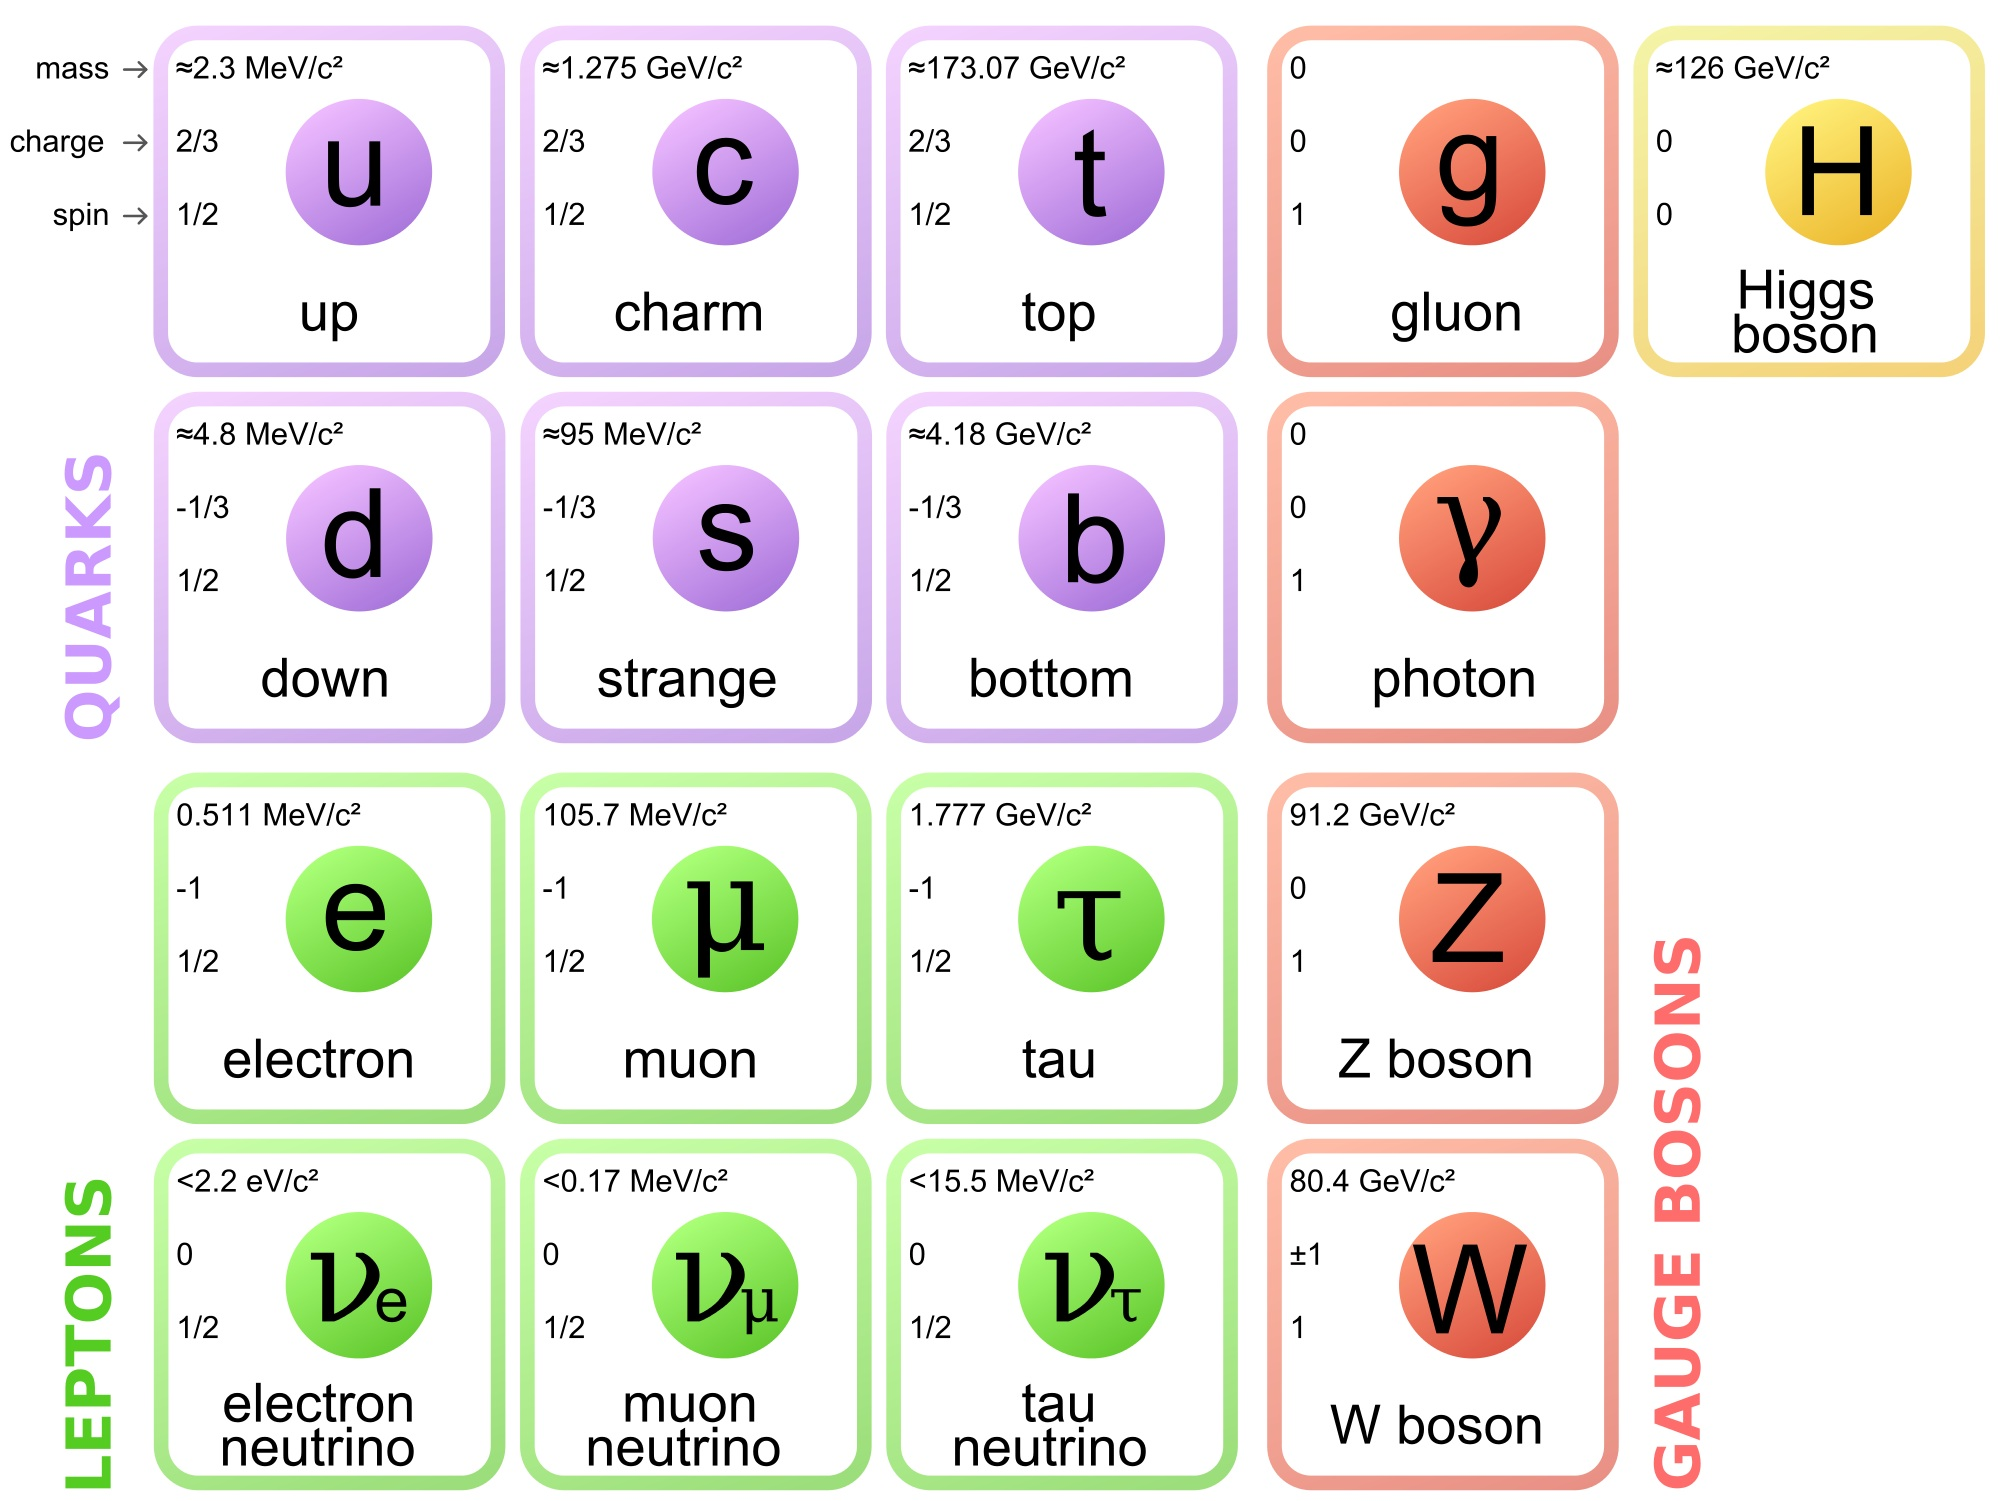
\includegraphics[width=0.8\textwidth]{Figures/standardmodel.jpg} 
 \caption{The current model of particle physics. Image courtesy of \cite{quantumdiaries}.}
\end{figure}

Similar to the electron ($e$), the muon carries a fundamental charge of $\pm$1, a spin of 1/2, and observes the electromagnetic and weak forces. Moreover, the muon also has a corresponding neutrino: the muon neutrino ($\nu_\mu$). However, the muon (mass = 105.7 MeV/$c^2$) is about 200 times heavier than the electron (mass = 0.511 MeV/$c^2$). Indeed, sometimes it is useful to think of a muon simply as a heavy electron, but the mass implies several unique characteristics. One of these are the instability of muons, since the following process is not forbidden by mass, charge, or lepton number conservation:
\begin{equation} \nonumber
\mu \rightarrow e+\bar{\nu_e}+\nu_\mu.\\
\end{equation}

This is quite interesting, as it means muons are a double-edged sword. On the one hand, their fundamentality means that the muon collisions will be clean. This is a great advantage over baryon collisions, since baryons are composed of three quarks (e.g. protons, neutrons). Consequently, any data from muon interactions will have relatively little noise and will not require the burden of jet analysis (as is sometimes the advantage of linear electron colliders). Yet unlike the electron, the muon does not emit a large amount of synchrotron radiation as it is accelerated. For this reason, it is possible to have a circular muon accelerator, and one far smaller than the equivalent baryon accelerator due to its small comparitive mass. On the other hand, a rest frame lifetime of 2 $\mu$s requires the muons to be accelerated before they decay. This is a challenge for circular colliders which require a high luminosity beam.

Now, it appears that there are several good advantages and only one disadvantage: the 2 $\mu$s mean rest frame lifetime of the muon. However, this is only a disadvantage for muon colliders. Another application which turns the moderately short lifetime into an advantage is that of a neutrino factory. The concept of a muon storage ring has existed since 1960 \cite{unpublishedring}, and its list of advantages only grows with time. 

%-------------------------------------------------------------------------------
\Section{COSY Infinity}\par
COSY Infinity is a beamline simulations tool used in the design, analysis, and optomization of particle accelerators \cite{cosy}. To do this, COSY uses the transfer map approach, which evaluates the overall effect of a system on a beam of particles  using differential algebra (involving multivariate Taylor polynomials up to arbitrary order). While a transfer map is technically not a nonlinear matrix, it is sometimes helpful to think of them as one in the same. Along with the evaluation of particles through a lattice, COSY also has a plethora of analysis and optomization tools, including (but not limited to) lattice aberration and correction tools, support for Twiss parameters, support for tunes and nonlinear tune shifts, built-in optimizers (for lattice design), and spin tracking. \par

COSY is particularly advantageous to use when considering the efficient use of computational time. This is due to the transfer map methods that COSY employs. Given some initial phase space vector $\mathbf{Z}(s_0)$ (see Figure \ref{fig:phaseSpaceVector}), the transfer map $\mathcal{M}$ will uniquely predict the time evolution of $\mathbf{Z}$. This is because most beam elements follow Maxwell's equations, which yield unique solutions that are dependent on initial conditions. Mathematically, this relationship is $\mathbf{Z}(s)=\mathcal{M}(s_0 , s)*\mathbf{Z}(s_0)$. Here, the independent variable $s$ is understood as the reference orbit (the zero point of a beam of particles in some comoving reference frame --see Figure \ref{fig:saxis}). An example of this relationship can be seen in Figure \ref{fig:matrix_element_example_1}. The initial phase space occupied by the beam of particles is at the coordinate $s_0$. Physically, there exists some deterministic beamline element. This element can be represented by the map $\mathcal{M}$, which creates a bijection for the phase space vectors $Z(s_0)$ and $Z(s)$ between the initial coordinate $s_0$ and an arbitrary final coordinate $s$. 

Valid elements are any beamline tools which are deterministic. Elements used in this study are magnetic multipoles (dipoles, quadrupoles, etc.), RF cavities, and drifts. Currently supported elements in COSY include but are not limited to: various magnetic and electric multipoles (with fringing effects), homogeneous and inhomogeneous bending elements, Wien filters, wigglers and undulators, cavities, cylindrical electromagnetic lenses, general particle optical elements, and deterministic polynomial absorbers of arbitrary order, with the last element being of particular interest.

\begin{figure}[h!]
\centering
$\mathbf{Z}=
\begin{pmatrix}
x\\ y\\ l=k(t-t_0)\\a=p_x/p_0\\b=p_y/p_0\\  \delta = (E-E_0)/E_0
\end{pmatrix}
$
\caption{Phase space vector $\mathbf{Z}$. Coordinates are transverse positions ($x, y$), time-of-flight in units of length ($l$), transverse angles w.r.t. the reference particle ($a, b$), and kinetic energy deviations w.r.t. the reference particle ($\delta$). The $0$ subscript in the definitions denotes the reference particle's properties.}
\label{fig:phaseSpaceVector}
\end{figure}

\begin{figure}[h!]
\centering
\includegraphics*[width=70mm]{./Figures/saxis}
\caption{The reference orbit.}
\label{fig:saxis}
\end{figure}


\begin{figure}[h!]
  \centering
    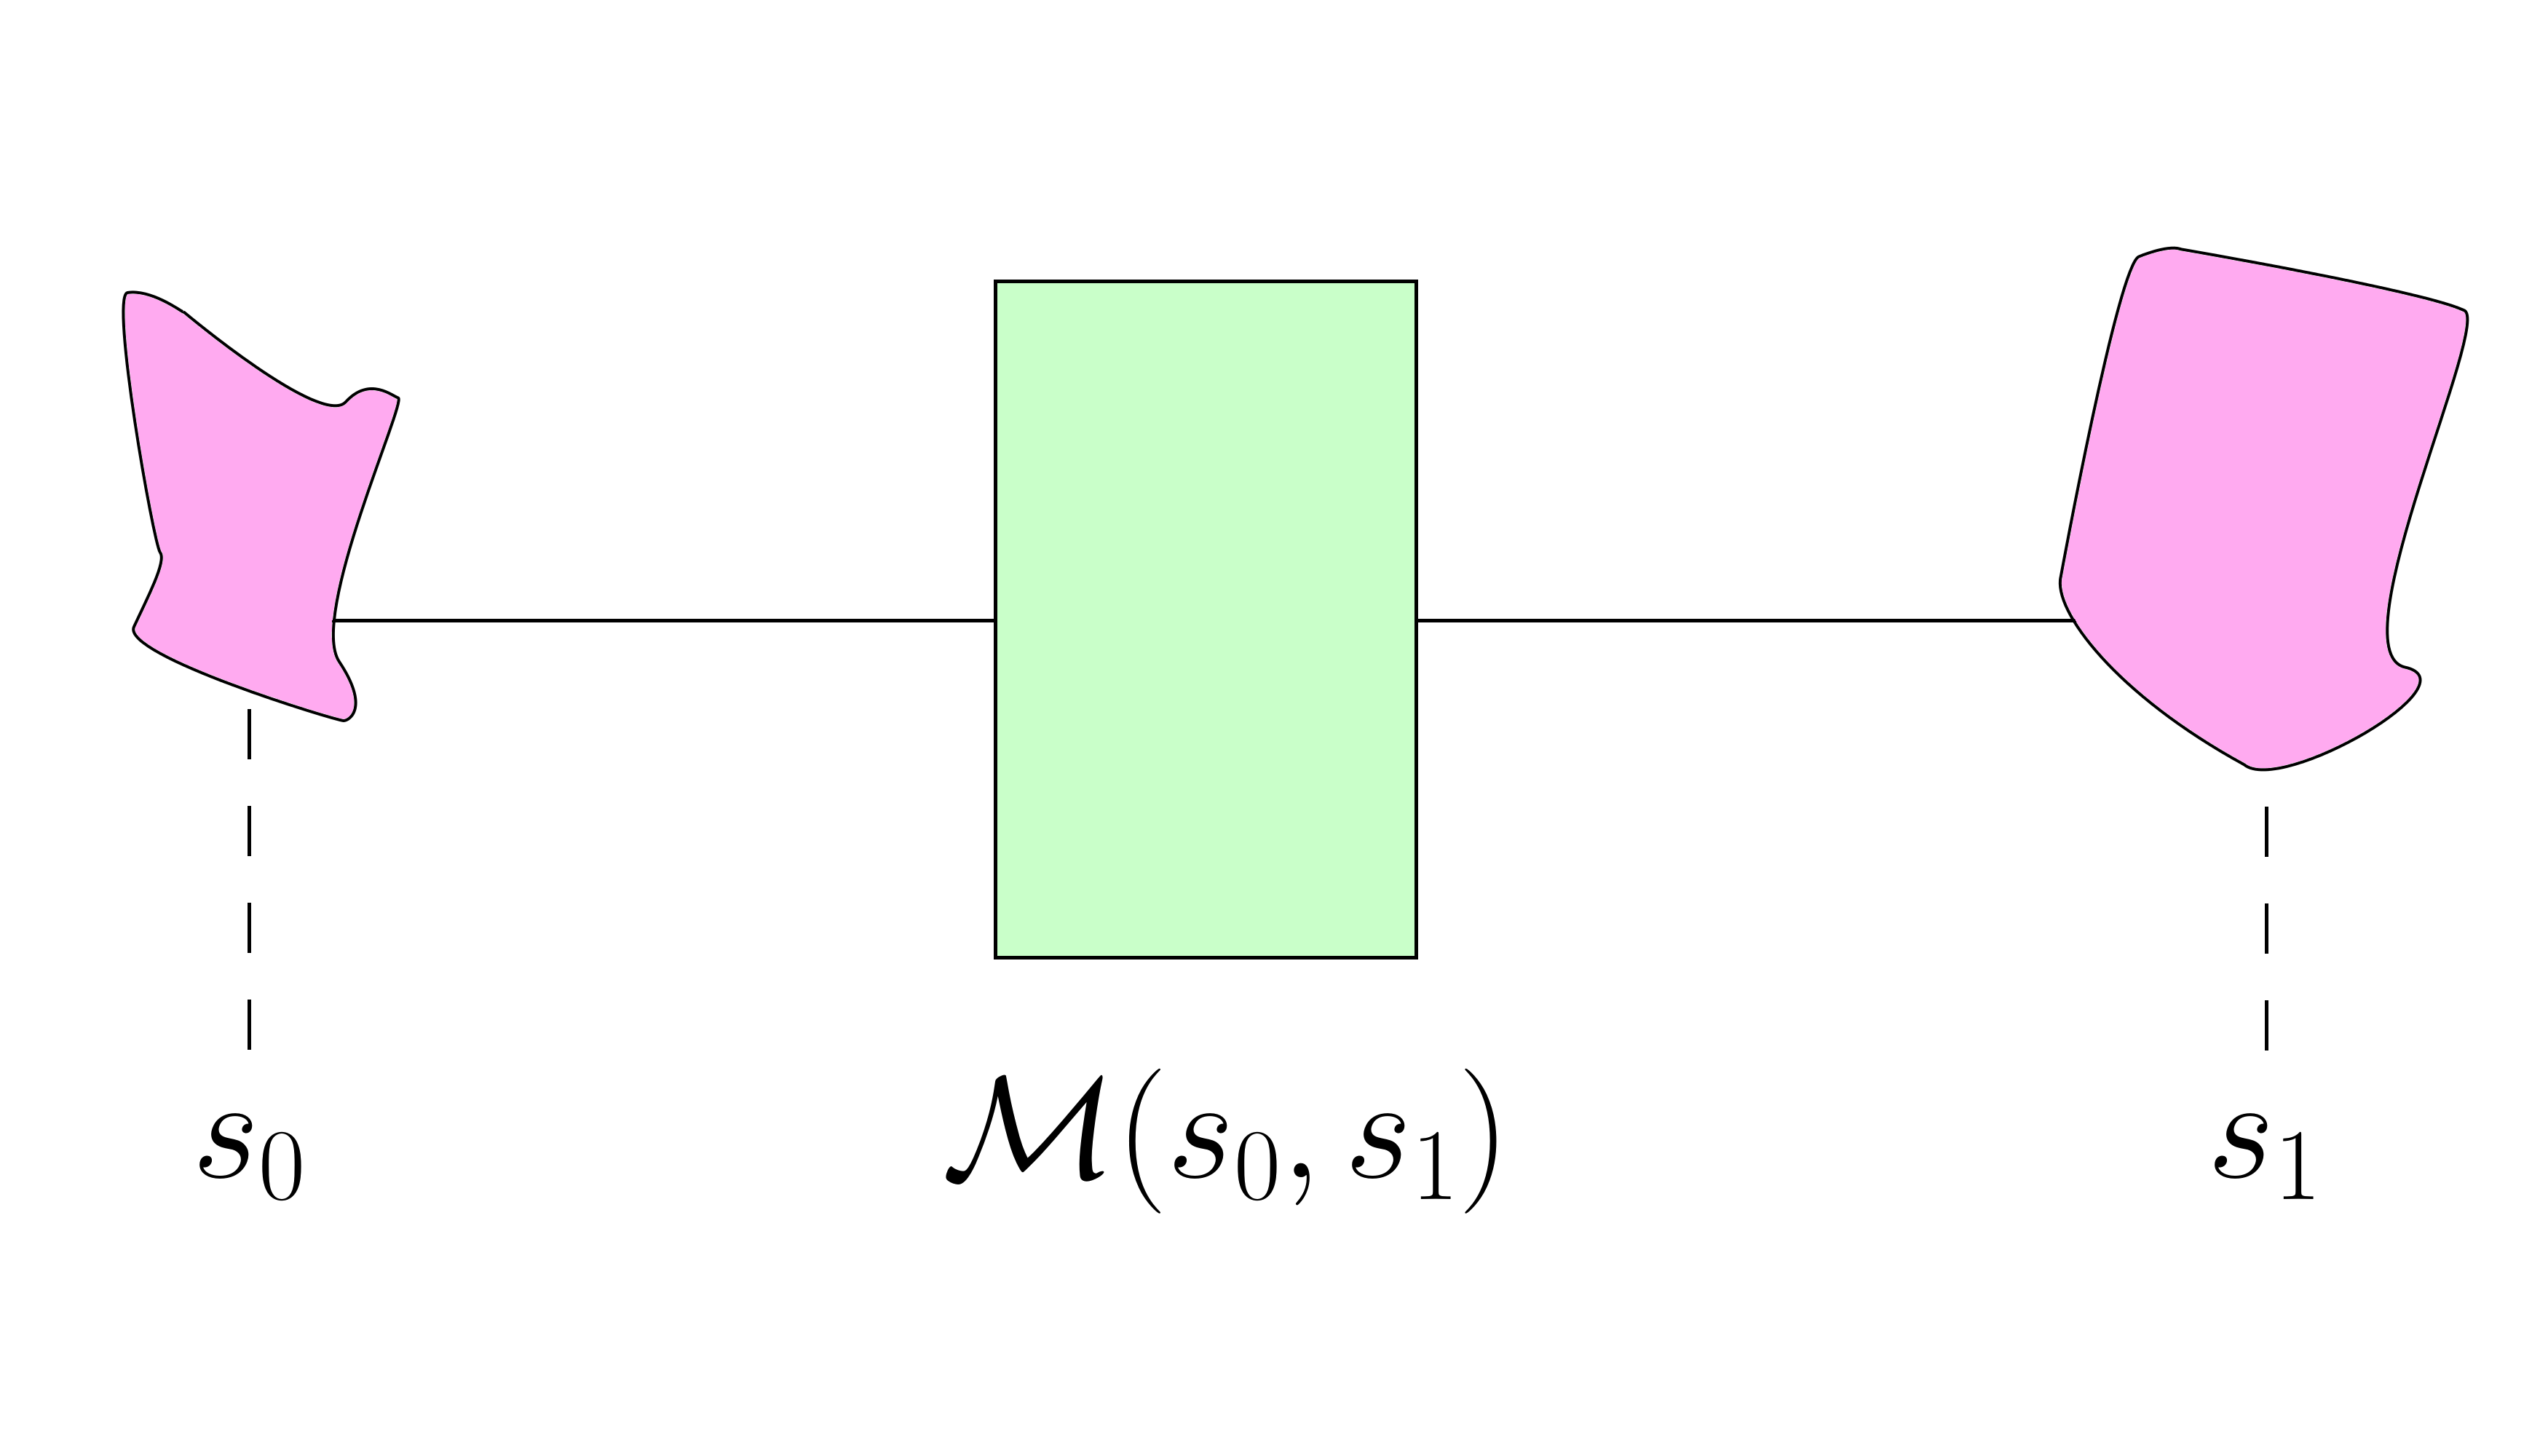
\includegraphics[width=0.75\textwidth]{Figures/matrix_element_example_1} 
  \caption{Example of some map $\mathcal{M}$ creating a bijection from $s_0$ to $s_1$.}
  \label{fig:matrix_element_example_1}
\end{figure}

Now, the composition of two maps yeilds another map: $\mathcal{M}(s_1 , s_2)\times \mathcal{M}(s_0 , s_1) = \mathcal{M}(s_0 , s_2)$. Therefore, it is possible to ``cut out" the middle part $s_1$. Since each physical lattice corresponds to some transfer map, it is possible to construct a single map that represents many individual lattices. An example of this can be seen in Figure \ref{fig:matrix_element_example_2}. Computationally this is advantageous because once calculated, it is much faster to apply a solitary transfer map to a distribution of particles than to simulate that same distribution through many meters of lattices.
\begin{figure}[h!]
  \centering
    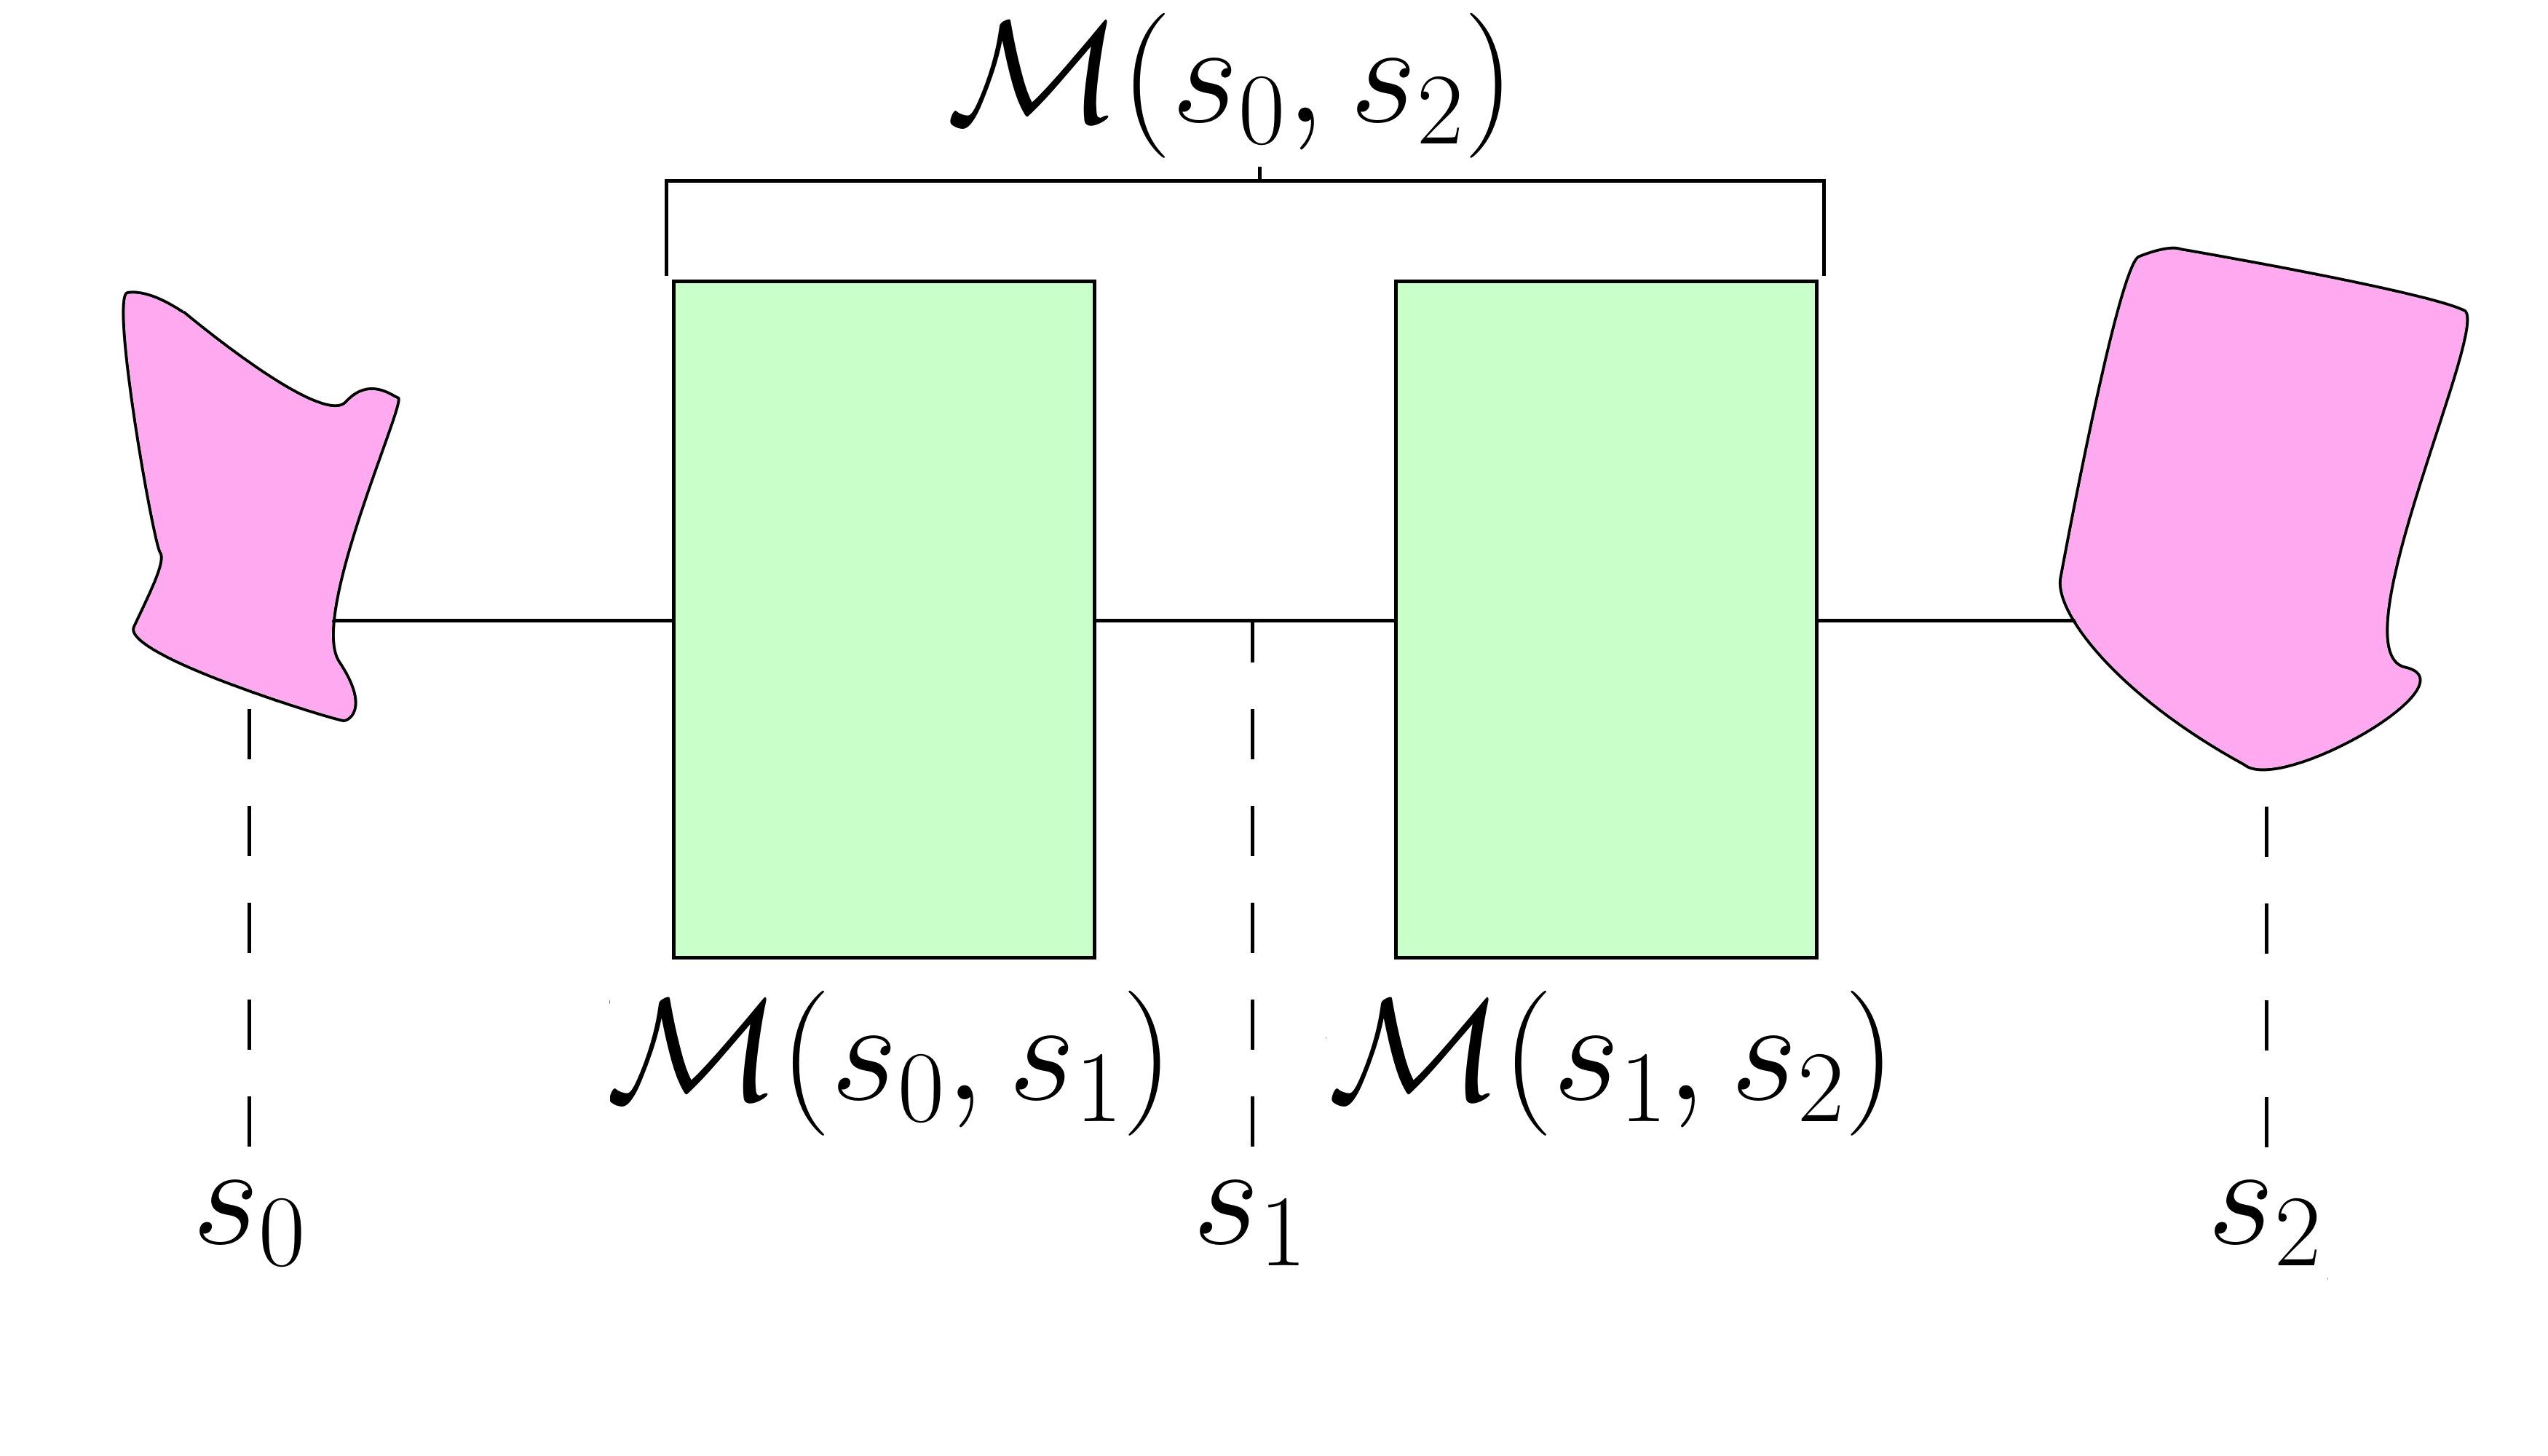
\includegraphics[width=0.75\textwidth]{Figures/matrix_element_example_2} 
  \caption{Example of two maps $\mathcal{M}(s_0,s_1)$ and $\mathcal{M}(s_1,s_2)$. These two maps may be multiplied together to reduce to a single map, $\mathcal{M}(s_0,s_2)$.}
  \label{fig:matrix_element_example_2}
\end{figure}
% Figure at the end of the section is bad!

%-------------------------------------------------------------------------------
\Section{Introduction to Matter-Dominated Lattices}\par

\Subsection{Introduction to Stochastic Effects}\par
This next section introduces stochastic effects, or effects which are intrinsically random. These are not to say effects which are deterministic, but approximated as random, as is the case in classical thermodynamics. In classical thermodynamics, a system has a very large number of particles. These particles and their evolution through time may be kept track of by a set of deterministic interactions (computational biophysics does this well with protein folding), but classically they are approxmated simply as a random set. In this sense, the large thermodynamic system is not stochastic, since it fails to be \emph{intrinsically} random. This is not the case with computational beam physics, as the models involved are typically require close range, dissipative forces, and quantum effects. It's not that the interactions are deterministic but difficult to keep track of, for that would require better bookkeeping or more precise measurements; rather the interactions are random by nature, deterministically unpredictable by no fault of the observer.

As discussed in the next section, this work is concerned with the interactions between a muon beam and some stationary target called the `absorber' --typically a cylinder or wedge filled with liquid hydrogen. The simplest model of a beam interacting with some stationary target can be found in several textbooks \cite{nielsen,griffithsqm}, but perhaps the most helpful model comes from \cite{jose} in Figure \ref{fig:scatteringmodel}.

\begin{figure}
  \centering
  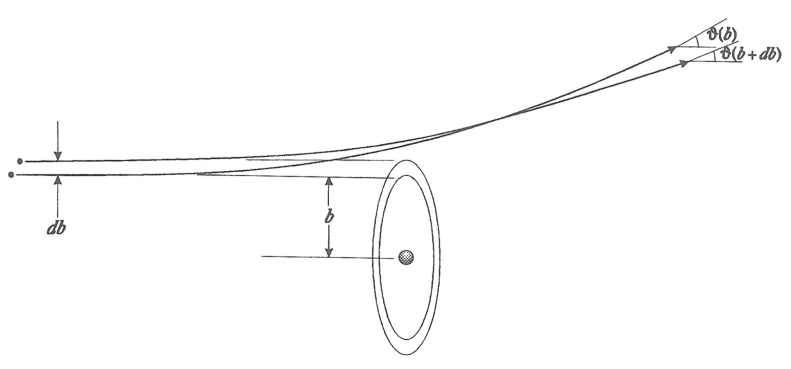
\includegraphics[width=\textwidth]{Figures/scattering_model} 

  \caption{Classical muon--target interaction model courtesy of \cite{jose}.}
  \label{fig:scatteringmodel}
\end{figure}

Here $b$ is referred to as the impact parameter and is measured with respect to the particle's initial trajectory. For a beam of noninteracting particles and a perfectly stationary target, classical mechanics suggest that this is a purely deterministic problem (see, e.g., `hard-sphere scattering' in \cite{griffithsqm}); the particle with a smaller impact parameter $b$ will deflect more than its neighbor with a slightly larger impact parameter of $b+db$. This model is entirely based on initial conditions, and if this were reality it would be relatively easy to implement these effects into the map methods of COSY Infinity. However, reality does not follow the model of Figure \ref{fig:scatteringmodel}. A more accurate model is illustrated by Figure \ref{fig:scatteringmodel2}. Here the target is still approximated as fixed, but the incident particle is now approximated as a travelling plane wave and the scattered particle is approximated as a spherical wave (at least locally).
\begin{figure}
  \centering
    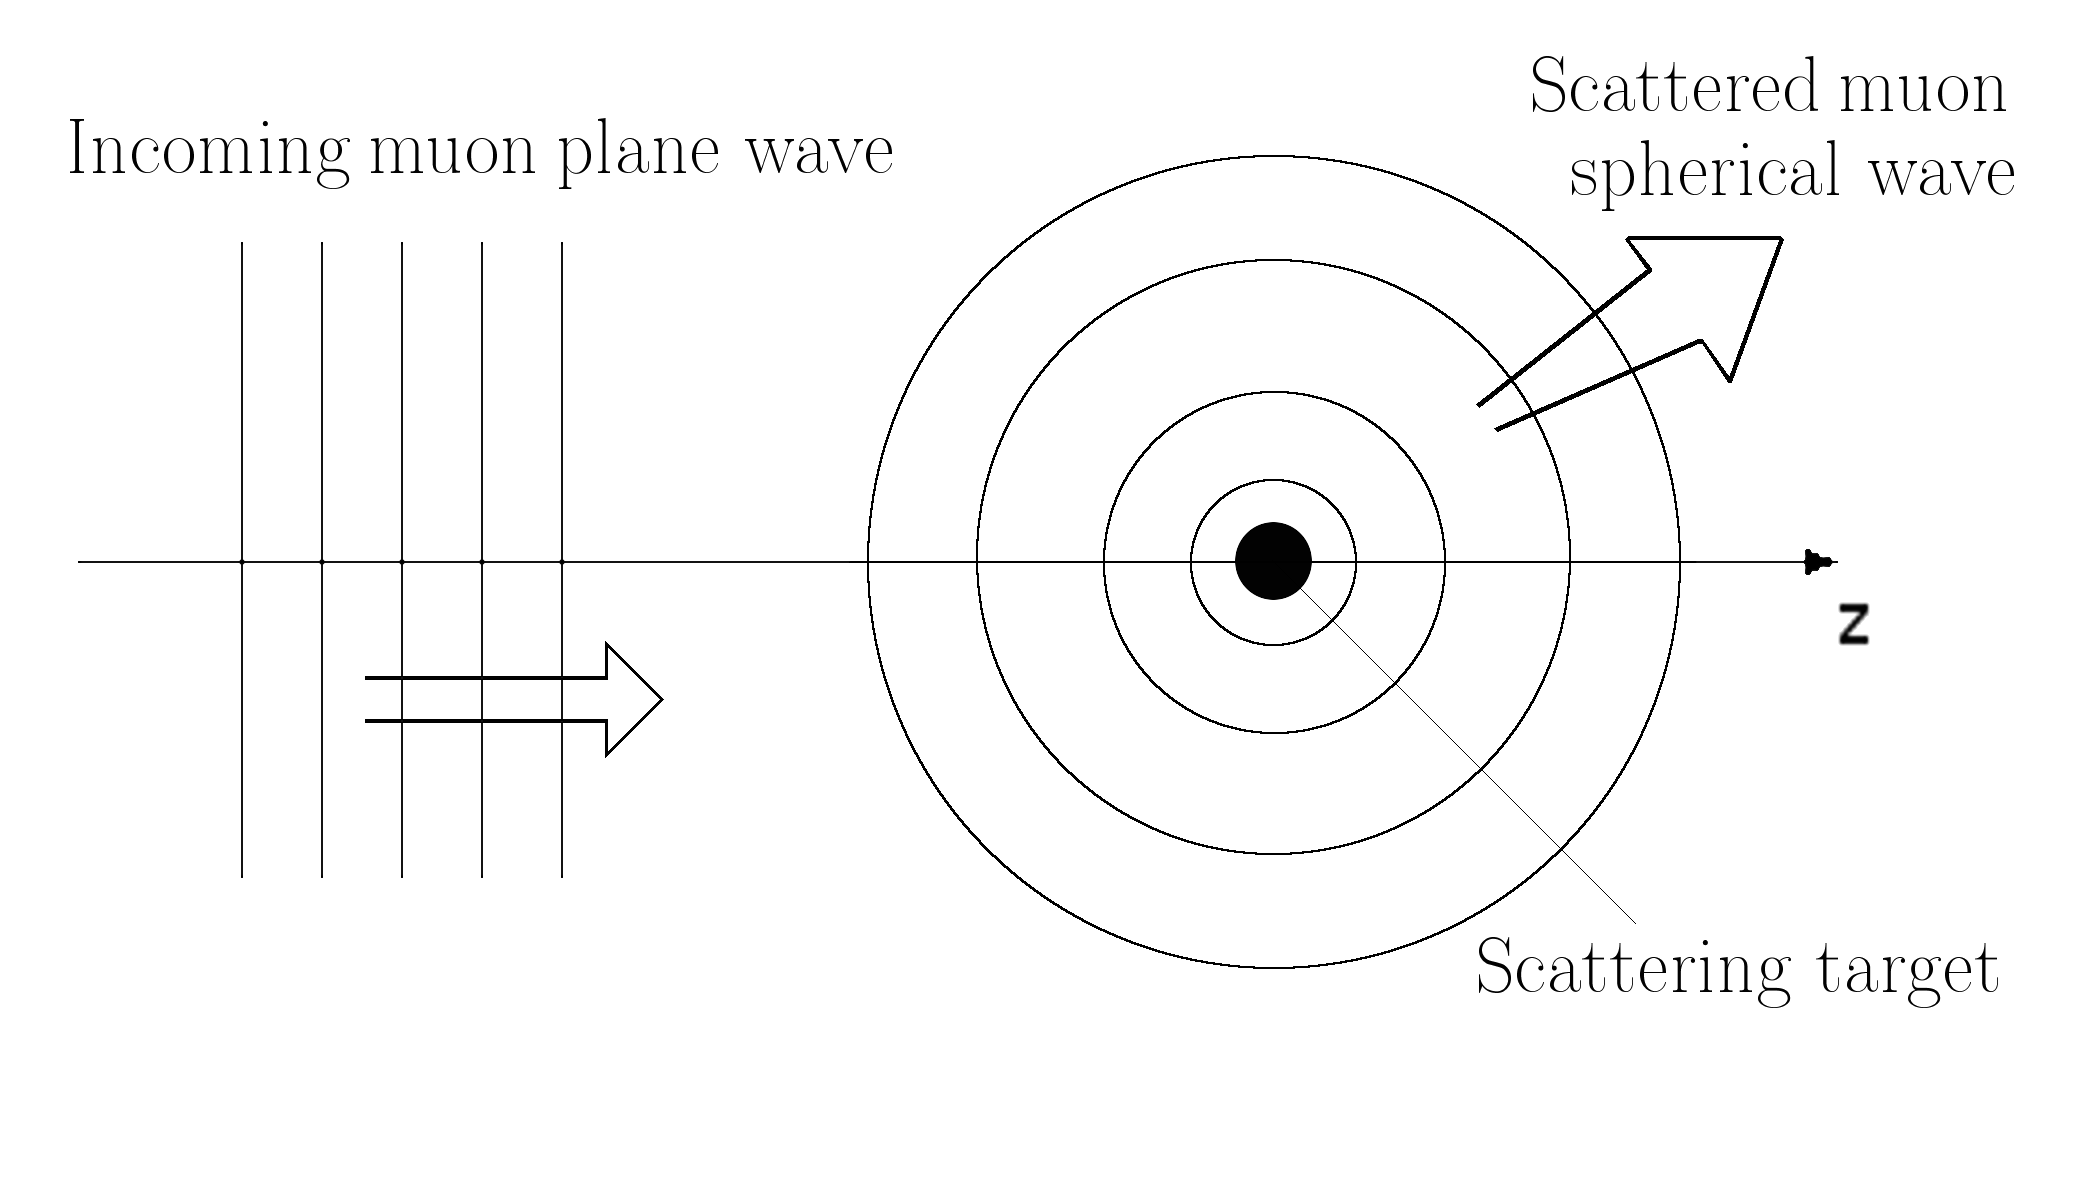
\includegraphics[width=\textwidth]{Figures/scattering_model_2} 
  \caption{Quantum muon-target interaction model. The incoming particle wavefunction is represented as a plane wave and is scattered locally as a spherical wave. Image courtesy of \cite{griffithsqm}.}
  \label{fig:scatteringmodel2}
\end{figure}
It will be shown later that this model predicts 
\begin{enumerate}
\item a spectrum of energy loss $\omega(\epsilon)$ which yields the probability of losing an amount of energy $\epsilon$ (see Section \ref{sec:ICOOLStraggling}), and
\item a scattering amplitude which gives the form of the probability of scattering in a given direction $\theta$ (see Section \ref{sec:ICOOLScattering}).
\end{enumerate}
Hence quantum theory suggests that even if two identical particles have identical initial conditions their final conditions will not be the same.

\Subsection{Muon Ionization Cooling}
In Section 1.1, the only real disadvantage to any muon-based accelerator was the mean muon rest frame lifetime (2 $\mu$s). This is expected to be far too short of a timespan to be useful in a traditional accelerator scheme. For the moment, observe the two proposed schematics in Figure \ref{fig:muon_accelerator_schematic}. The section labelled `Proton Driver' produces the source protons, which will eventually produce muons. This is essential since muons do not naturally occur in great quantities at a convenient extraction point. These protons then strike some large target (which must be optimized to produce the highest yield), resulting in a spray of protons, muons, electrons, and pions (even shorter-lived particles consisting of a quark-antiquark pair). To further optimize this process, it is advantageous to let the pions decay into muons via $\pi^\pm \rightarrow \mu^\pm + \nu_\mu$. The large assemblage of muons is then split up into bunches and propagated through the phase rotator. The next section is where all of the interesting physics lies, and is the topic of this entire thesis. For now, it will be simply addressed as the `cooling channel' and delved into later. Cooling simply means to reduce the bunch's transverse phase space --that is, it means to limit the beam's immediate physical size and possible future physical size in the transverse direction. The purpose of this is to increase the luminosity of the resulting beam; for a collider, this means more collisions; for a neutrino factory, this means more neutrino counts in the detectors (since neutrinos are neutral, the $\nu$ beam would otherwise tend to disperse). After this critical step, the beam accelerates to an appropriate energy. For a neutrino factory, this is 5 GeV, and the muon and antimuon beams are allowed to decay in a storage ring. For a muon collider, the center-of-momentum energy is $\sim$ 126 GeV for a Higgs factory or up to 10 TeV with current technology for high energy studies.

\begin{figure}
  \centering
    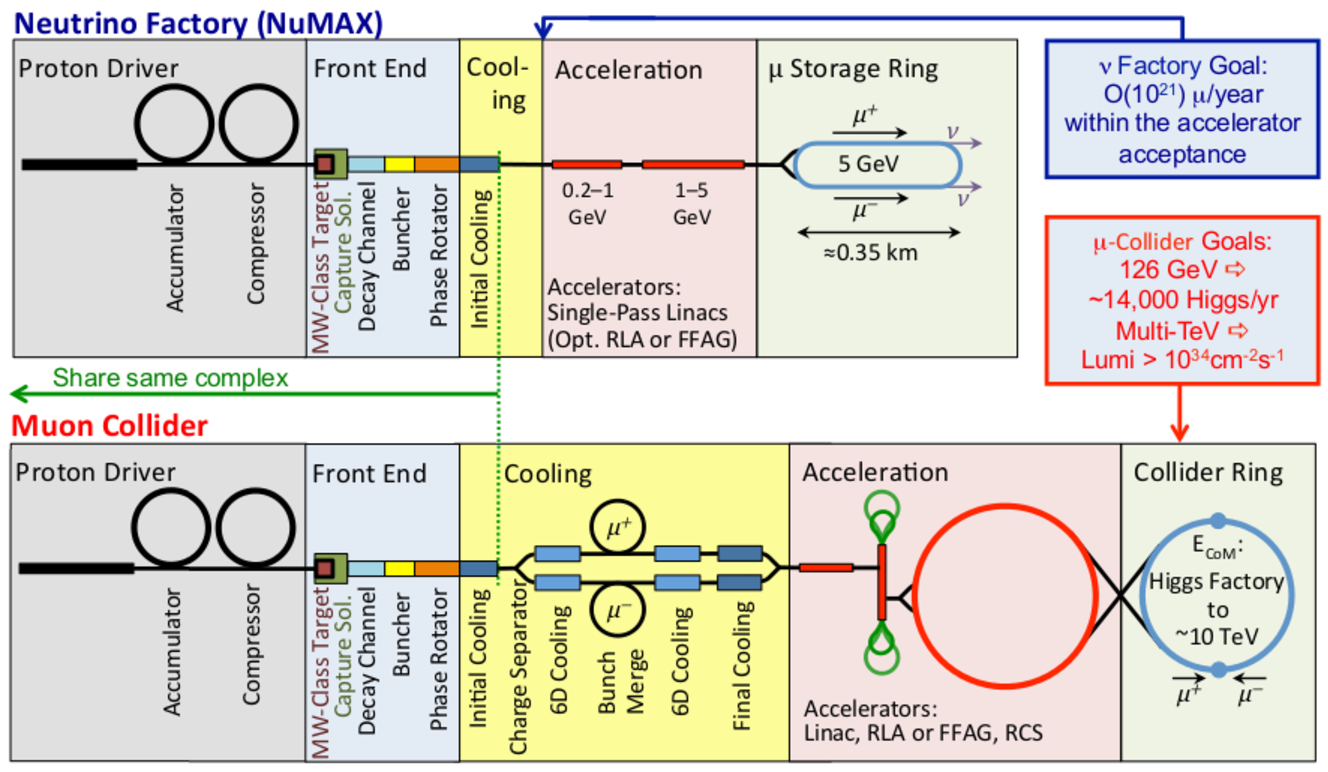
\includegraphics[width=\textwidth]{Figures/muon_accelerator_schematic} 
  \caption{Proposed muon accelerator shematics.}
  \label{fig:muon_accelerator_schematic}
\end{figure}


The cooling channel is the crux of the entire operation for either purpose. Traditional cooling methods (e.g. FODO, electron cooling, etc.) are expected to take far too long to allow a significant portion of the muon beam to survive. For example, for 1 $TeV$ muons the mean muon lifetime in the lab frame is $\bar{t'}=2.2 \mu s$ $\cdot$ 1 $TeV/$ 105.7 $MeV \approx 0.02s$.
 However, ionization cooling is a much faster method. Ionization cooling requires the beam to deposit its energy in matter, thus ionizing the matter. This reduction of total energy in the beam diminishes its phase space in all three directions: ($x, P_x$), ($y, P_y$), and ($z, P_z$). For this reason, it is sometimes also called 6D cooling. 

While the idea of ionization cooling has been around since at least 1956 \cite{oneill,lichtenberg}, it did not appear to be a viable option until roughly 1970 \cite{YuM}. It was believed that the multiple scattering effect would mask any cooling benefits. Scattering is a quantum effect which deflects two objects when they are in close proximity at high energies, and hence is intrinsically random. This means that while the energy deposition reduced the beam's phase space, the beam would also grow in the transverse direction due to this multiple scattering. This phenomenon is now known as phase space exchange or emittance exchange.

Now, this seems to be quite the opposite of what is intended; ionization cooling produces a slow, fat beam, and a good muon beam should be narrow and fast so that the Lorentz boost keeps the muons from decaying. Fortunately, there exists a schematic that solves both of these problems simultaneously. Physically, it is represented in  Figure \ref{fig:coolingchannel} and it is vectorally depicted in Figure \ref{fig:123ionization}.
\begin{figure}
  \begin{center} 
    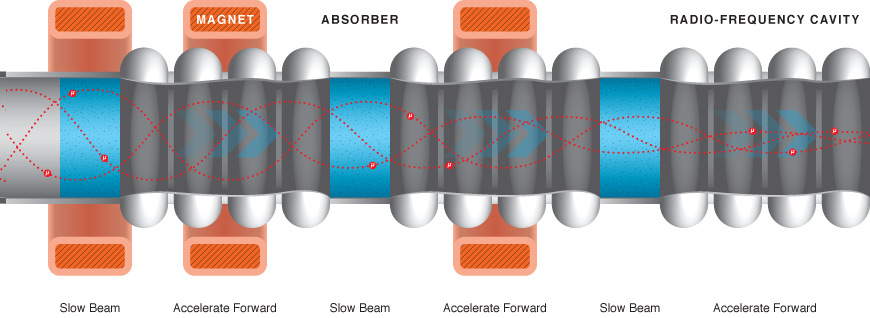
\includegraphics[width=\textwidth]{Figures/coolingchannel} 
  \caption{Cartoon of a cooling channel.}
  \label{fig:coolingchannel}
 \end{center}
\end{figure}

The key is to use a cell which contains both the ionizing material and a radio frequency cavity. It is clear why this solves the latter problem: after the beam loses energy, it gains that much energy again, and so the Lorentz boost stays roughly constant. However, to understand why this solves the former problem it is necessary to observe Figure \ref{fig:123ionization}. In Figure \ref{fig:123ionization}, the longitudinal momentum ($p_l$) is plotted against the transverse momentum ($p_t$). 
   \begin{enumerate} 
  \item{Beam deposits energy in material, reducing the momentum in both directions.}
  \item{Multiple scattering effects are observed. The transverse direction increases (or `heats up'). }
  \item{The beam is re-accelerated by the RF cavity, increasing the longitudinal momentum only. The result is a reduction in transverse momentum (i.e. blue vector compared to black vector).}
\end{enumerate}

\begin{figure}
  \centering
   \captionsetup{singlelinecheck=off}
    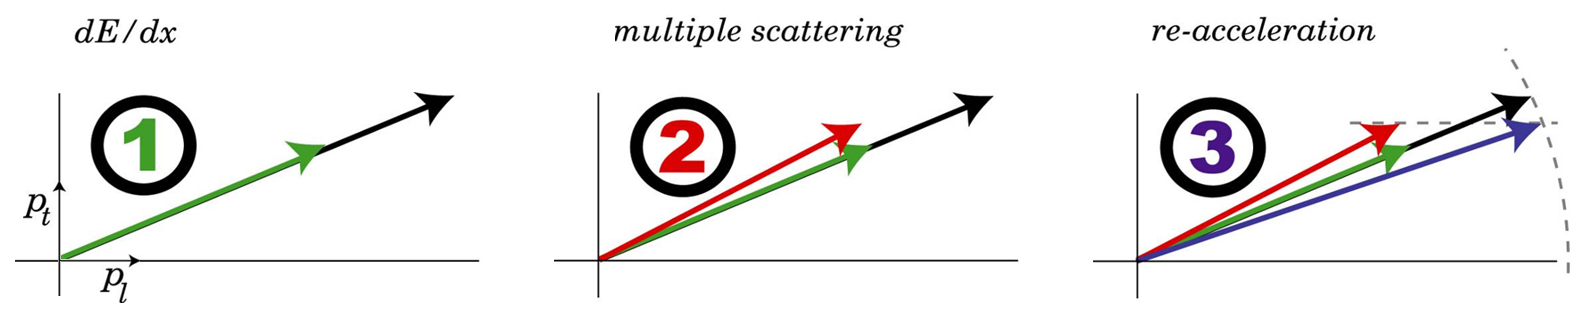
\includegraphics[width=\textwidth]{Figures/123ionization} 
  \caption{Vectoral depiction of ionization cooling in Figure \ref{fig:coolingchannel}. }
  \label{fig:123ionization}
\end{figure}

%-------------------------------------------------------------------------------------------------------------------------------------------------

\Subsection{Emittance}
Often, it is advantageous to represent the volume of phase space occupied by the beam as the emittance, $\epsilon$. Moreover, this volume should be normalized by the usual relativistic factors, $\gamma$ and $\beta$. For the relevant transverse emittance,
%
\begin{equation}
\label{eqn:emittancedef}
%\epsilon_x^N=\beta\gamma\epsilon_x=\beta \gamma\sigma_x \sigma_\theta.
\epsilon_x^N=\beta\gamma\epsilon_x=\beta\gamma\sqrt{\left<x^2\right>\left<\theta^2\right>-\left<x\theta\right>^2}.
\end{equation}
%
Here, azimuthal symmetry is assumed, and so $x$ represents the general transverse position, and $\theta$ is the projection of the divergence angle of the particle trajectory onto the $x$-$z$ plane. 

It is conceptually easy to understand why this represents a volume of phase space. Since the `beam' is a collection of particles, its full width is not simply defined. For this reason, the width of the beam is represented as the beam's RMS. Provided that the beam is nearly Gaussian, if there existed no cross-dependence in $x$ and $\theta$, then the picture should look like the left side of Figure \ref{fig:ellipses}. Then the volume of this bivariate Gaussian is proportional to $\sqrt{\left<x^2\right>\left<\theta^2\right>}$. However, if there is some cross-dependence (right side of Figure \ref{fig:ellipses}) then this must be accounted for by subtracting the cross term from the RMS terms.

\begin{figure}
  \begin{center}
    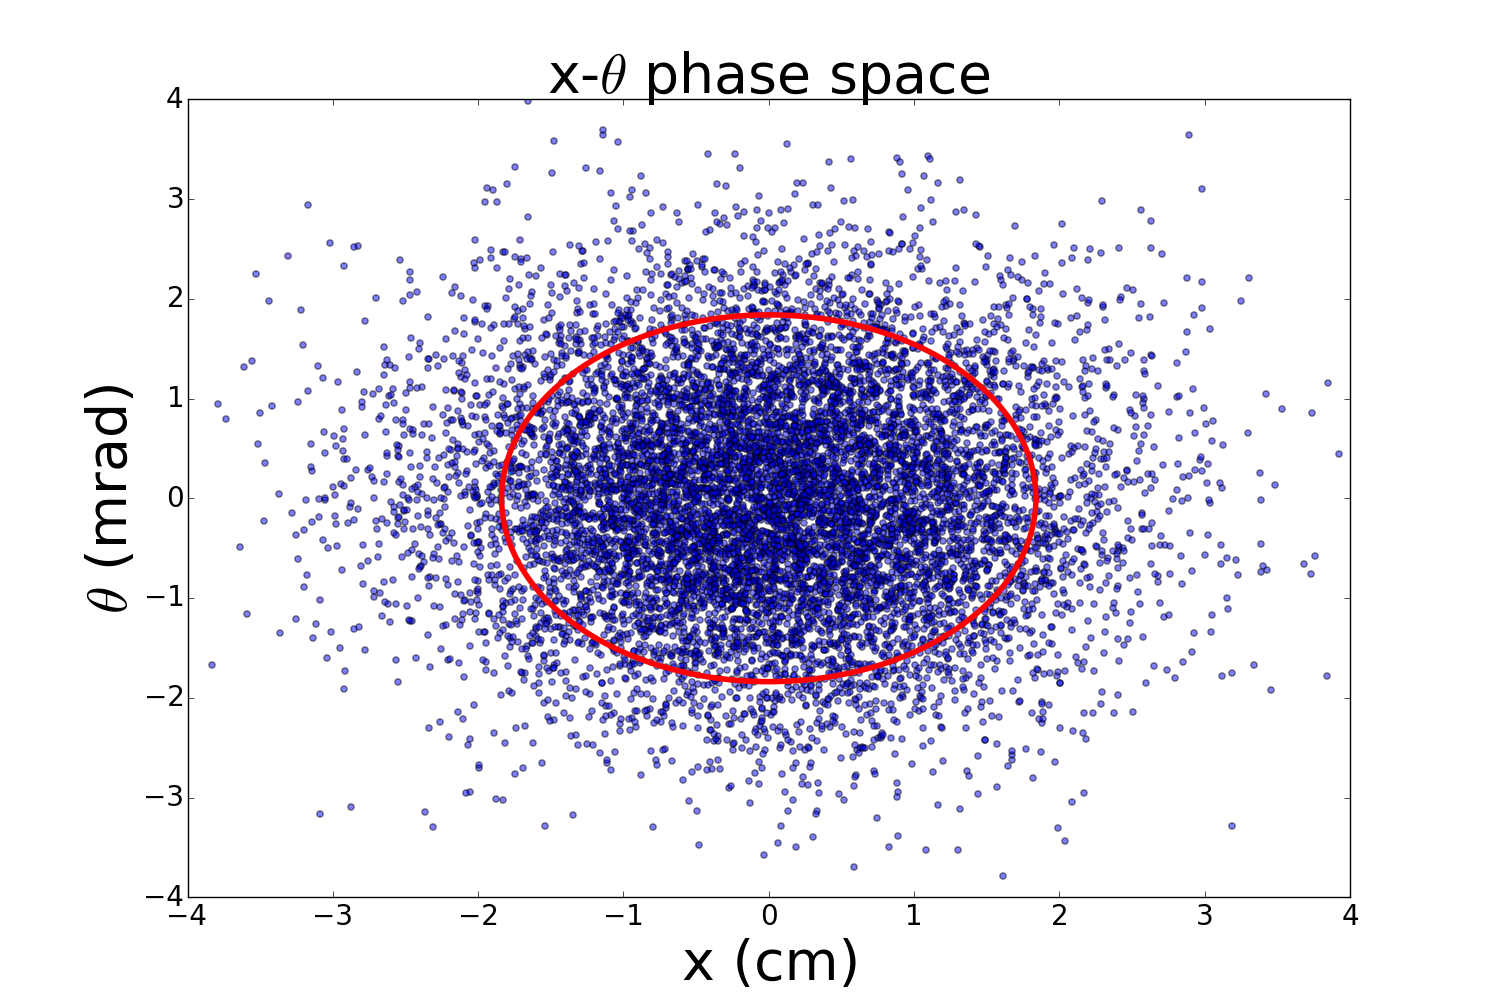
\includegraphics[width=0.49\textwidth]{Figures/ellipse0} 
    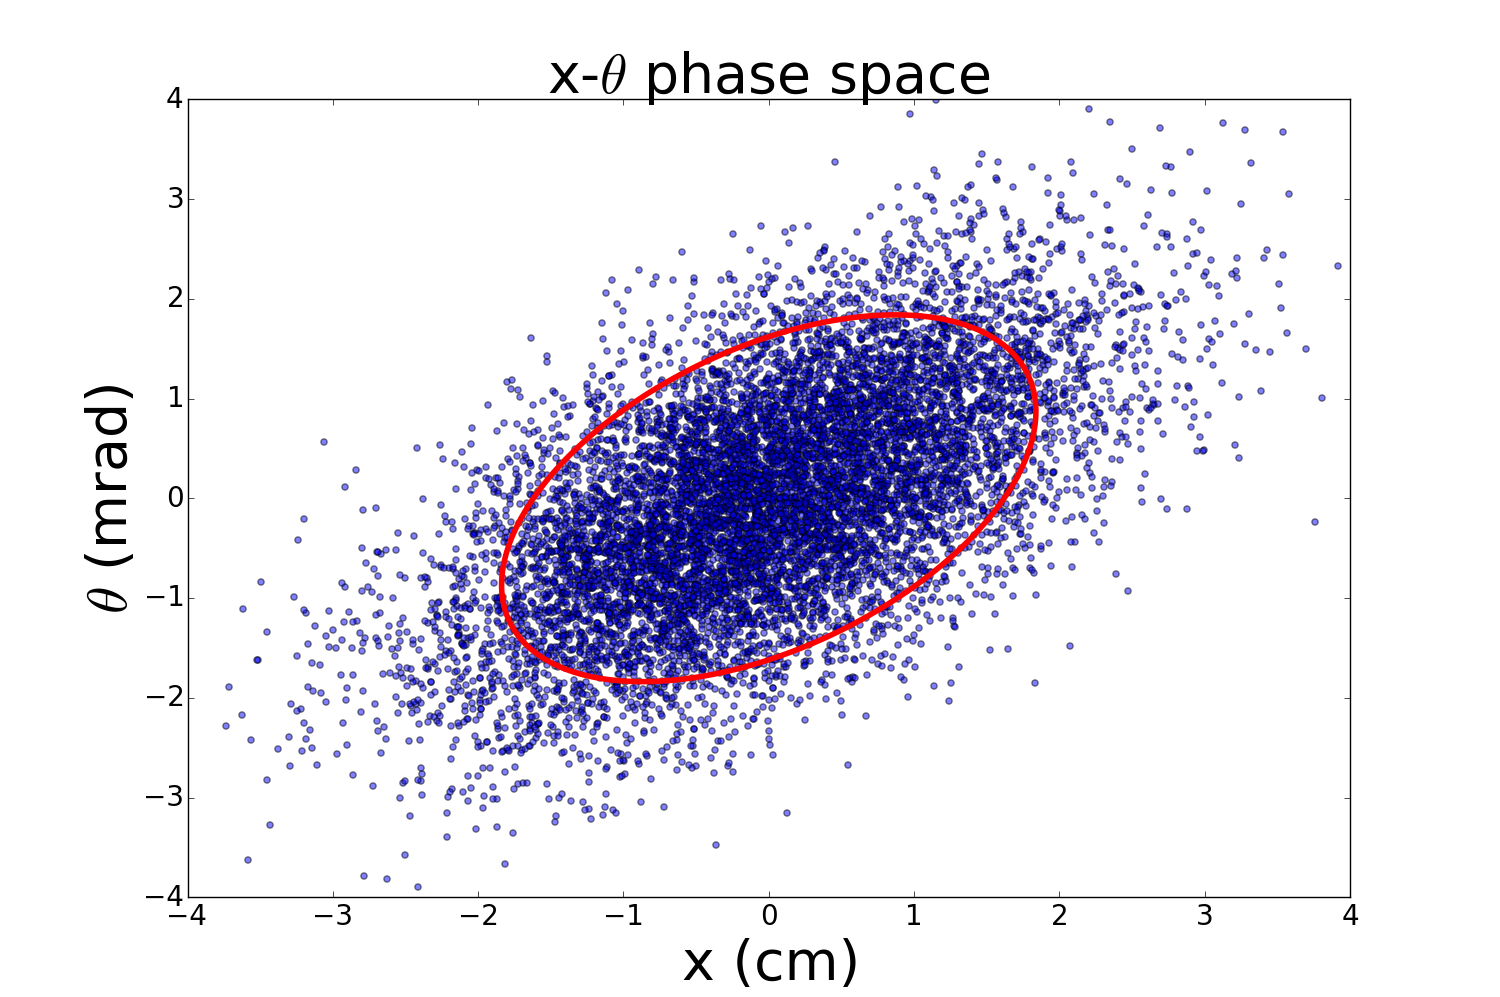
\includegraphics[width=0.49\textwidth]{Figures/ellipse1} 
  \caption{Left: example beam with no $x$-$\theta$ correlation. Right: example beam with significant $x$-$\theta$ correlation.}
  \label{fig:ellipses}
 \end{center}
\end{figure}

Now it is possible to derive the effect of cooling absorbers on emittance as it pertains to muon ionization cooling. Closely following \cite{Fernow}, Eqn. \ref{eqn:emittancedef} is differentiated by $z$:
%
\begin{equation}
\label{eqn:emittance1}
\frac{d\epsilon_x^N}{dz}=\epsilon_x \frac{d(\beta\gamma)}{dz}+\beta\gamma\frac{d\epsilon_x}{dz},
\end{equation}
%
It will soon be shown that the first term represents `cooling' and the second term represents `heating' in the transverse plane. Starting with the heating term,
%
\begin{equation} \nonumber
\frac{d\epsilon_x^N}{dz}(heat)=\beta\gamma\frac{d\epsilon_x}{dz}.
\end{equation}
%

It can be assumed that the cooling is taking place near the beam waist (that is, the part of the trajectory where the beam is smallest). For this case, it is a reasonable approximation that the transverse phase space looks more similar to the left side of Figure \ref{fig:ellipses}, and so the $\left<x\theta\right>$ term may be neglected. Furthermore, with strong focusing it is possible to neglect the rate of position growth of the beam (this is cited in \ref{Fernow} provided the conditions that $\sigma_{xo}^2 \gg \theta_c^2 L / 2\omega^2$ and $\sigma_{xo}^2 \gg \theta_c^2 / 4\omega^3$, where L is the absorber length, $\omega$ is the focusing strength parameter, $\sigma_{xo}$ is the original beam size incident upon the absorber, and $\theta_c$ is the coefficient of the RMS scattering angle given in \cite{highland}). Using these two approximations, the only derivative in the heating term is that by $\left<\theta^2\right>$:
\begin{equation} \nonumber
\frac{d\epsilon_x^N}{dz}(heat)\approx\beta\gamma\frac{d}{dz}\sqrt{\left<x^2\right>\left<\theta^2\right>}\approx \frac{\beta\gamma}{2\epsilon_x}\left<x^2\right>\frac{d}{dz}\left<\theta^2\right>.
\end{equation}

From betatron focusing theory, $\left<x^2\right>$ may be rewritten as $\beta_\perp \epsilon_x$. Moreover, using \cite{highland} $\left<\theta^2\right>$ can be written as $h(z)/\beta^2E$. Here, $h(z)$ is the Highland $z$-dependence, the form of which many theories disagree. However, the first order term of $h(z)$ is generally not model-dependent, and so this becomes
\begin{equation} \nonumber
\left<\theta^2\right>\approx\frac{E_s}{\beta^2 E}\sqrt{\frac{z}{X_0}},
\end{equation}
where $E_s$ is some characteristic energy ($\approx14$ $MeV$) and $X_0$ is the radiation length of the given material. Then
\begin{equation} \nonumber
\frac{d\epsilon_x^N}{dz}(heat)\approx\beta\gamma\frac{\beta_\perp}{2}\frac{d}{dz}\big(\frac{E_s}{\beta^2 E}\sqrt{\frac{z}{X_0}}\big),
\end{equation}

\begin{equation}
\label{eqn:emittanceheat}
\frac{d\epsilon_x^N}{dz}(heat)\approx\frac{\beta_\perp}{2}\frac{E_s^2}{\beta^3Emc^2}\frac{1}{X_0}.
\end{equation}

Now it is clearer why this is referred to as the heating term. Since the derivative of emittance is positive, this part represents emittance growth. Moreover, to reduce this growth it is necessary to have highly energetic particles through a material with a large radiation length (typically $X_0 \propto Z$ (nuclear charge)).

Observe the cooling term of Eqn. \ref{eqn:emittance1}:
\begin{equation} \nonumber
\frac{d\epsilon_x^N}{dz}(cool)=\epsilon_x\frac{d(\beta\gamma)}{dz}=\epsilon_x\cdot(\beta\frac{d\gamma}{dz}+\gamma\frac{d\beta}{dz}).
\end{equation}
First,
\begin{equation} \nonumber
\frac{d\beta}{dz}=\frac{d}{dz}(1-\gamma^{-2})^{\frac{1}{2}}=\frac{1}{\beta\gamma^3}\frac{d\gamma}{dz},
\end{equation}
and then,
\begin{equation} \nonumber
\frac{d\gamma}{dz}=\frac{\gamma}{E}\frac{dE}{dz},
\end{equation}
with $E$ as the total energy of the muon beam. Finally,
\begin{equation} \nonumber
\frac{d\epsilon_x^N}{dz}(cool)=\epsilon_x\cdot(\beta\frac{d\gamma}{dz}+\gamma\frac{1}{\beta\gamma^3}\frac{d\gamma}{dz})=\epsilon_x\cdot\frac{d\gamma}{dz}\beta(1+\frac{1}{\beta^2\gamma^2}) \vspace*{12pt}
\frac{d\epsilon_x^N}{dz}(cool)=\epsilon_x\frac{dE}{dz}\frac{\gamma}{E\beta}.
\end{equation}
Normalizing the emittance by first multiplying and then dividing by $\beta\gamma$ results in
\begin{equation} \nonumber
\frac{d\epsilon_x^N}{dz}(cool)=\frac{1}{\beta}\frac{dE}{dz}\frac{\epsilon_x^N}{E}
\end{equation}
However, there are two notations which should be observed. First, even for a perfect monoenergetic pencil beam energy loss is stochastic, not deterministic. Two muons with identical initial conditions will likely lose different amounts of energy as they pass through the same medium. Since emittance is a collective effect, is it more appropriate to talk about an average energy loss, which turns $\frac{dE}{dz}$ into $\left<\frac{dE}{dz}\right>$. The second observation is with regard to sign convention. Typically, one refers to energy loss as a positive quantity (e.g. the beam lost 10 MeV from point A to point B), even though it is clear that $\frac{dE}{dz}$ is a negative quantity. For this reason, the energy loss term must again be changed from $\left<\frac{dE}{dz}\right>$ to  $-\left|\left<\frac{dE}{dz}\right>\right|$. This leaves the full cooling term as
\begin{equation}
\label{eqn:emittancecool}
\frac{d\epsilon_x^N}{dz}(cool)=-\frac{1}{\beta}\left| \left<\frac{dE}{dz}\right>\right| \frac{\epsilon_x^N}{E}.
\end{equation}

Similar to the heating term, it is now understandable why this is referred to as the cooling term. The rate of change of the normalized transverse emittance is negative, and so the transverse phase space shrinks. However, at this point Eqn. \ref{eqn:emittancecool} does not explain precisely how the rate changes, and so is purely conceptual for the time being. The shape of the cooling term is determined by the average energy loss, $\left|\left<\frac{dE}{dz}\right>\right|$. However, usually it is not $\left|\left<\frac{dE}{dz}\right>\right|$ that is measured, but rather the stopping power $S(E)=-\frac{1}{\rho}\left<\frac{dE}{dx}\right>$, typically in units of $MeV$ $cm^2/g$. A good example of a stopping power curve can be seen in Figure \ref{fig:bethecurve} \cite{PDG}. For this example, there are several effects noted in Figure \ref{fig:bethecurve}, and one may be tempted to think that based on \ref{eqn:emittancecool} the most cooling should occur in the Anderson-Ziegler regime at $\beta\gamma\sim0.01$ (since there is a $1/E$ dependence in Eqn. \ref{eqn:emittancecool}, the high energy part of the curve does no good). Indeed, for $\rho= 8.92$ $g/cm^3$ it is easy to see that at $\beta\gamma=0.01$ then $\frac{d\epsilon_x^N}{dz}(cool)\approx-900$  $cm^{-1} \cdot \epsilon_x^N$ .

However, the correct strategy is just the opposite --one should endeavor to build a cooling cell with the minimum ionization point in mind (in the Bethe regime, where $\beta\gamma\sim2$). At the peak ($\beta\gamma\sim0.01$), the muon beam slows down quite a bit through a single cooling cell and one is at risk of losing their beam to decay. Moreover, Figure \ref{fig:bethecurve} only depicts the stopping power, not the actual energy loss that individual particles experience. The individual energy loss is a stochastic effect, and the distribution of energy losses broadens with decreasing beam energy. This means that for lower energies, there will be more particles which stop completely. Further, with a higher beam energy the stochastic energy loss profile is more sharply peaked, and so there are fewer decays and more particles which fall into the RF bucket. (Remember, the longitidunal emittance is observed by the RF cavities, as seen in Figure \ref{fig:coolingchannel}. The longitudinal emittance increases with energy loss according to \cite{Fernow}.) Finally, it is apparent in Eqn. \ref{eqn:emittanceheat} that higher energies are better, since they reduce the heating term. For these reasons, it is apparent that a muon cooling cell should be made of low $Z$ materials such as liquid hydrogen or lithium hydride and operate anywhere between 100 $MeV$/c to 400 $MeV$/c.

\begin{figure}
  \centering
    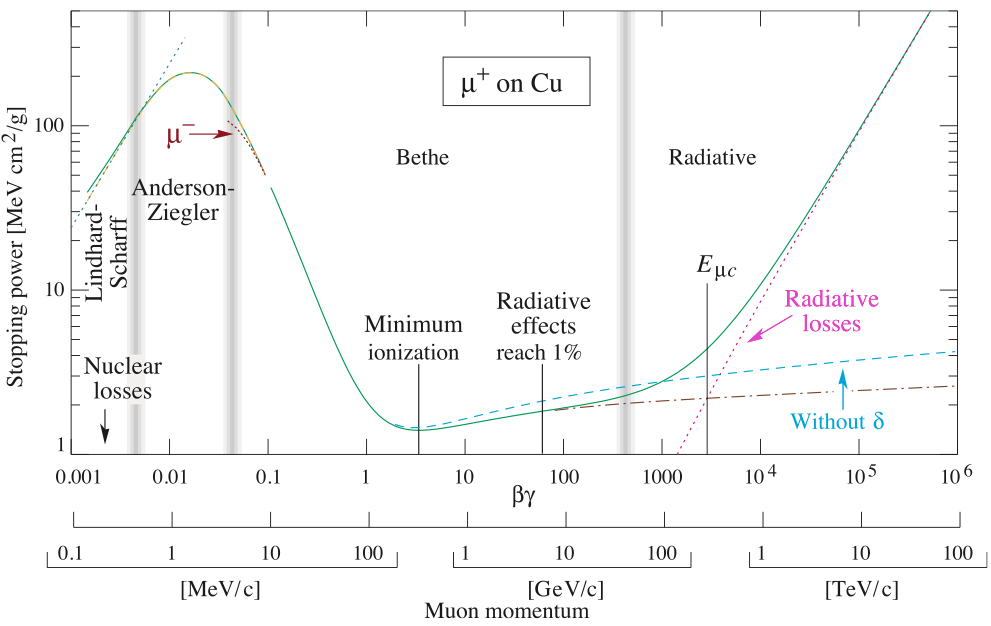
\includegraphics[width=\textwidth]{Figures/bethecurve} 
  \caption{Stopping power curve for antimuons on copper, courtesy of \cite{PDG}. }
  \label{fig:bethecurve}
\end{figure}

When particles impinge upon a fixed target, they lose some of their energy. For massive particles like muons, there are four major effects which contribute to this energy loss: ionization, bremsstrahlung radiation, pair production, and photonuclear interactions. However, it is important to note that in the muon cooling regime only ionization contributes significantly to the energy loss. To see this, take for an example the relatively heavy element of iron (iron is chosen because it is a fairly relatable element to those who are not experts in this field). In Figure \ref{fig:elossfe}, the energy loss contributions of these four effects can be seen. However, the non-ionization effects only start to contribute at an initial beam kinetic energy of 1.40 $GeV$ --far outside of the muon cooling regime.

\begin{figure}
  \centering
    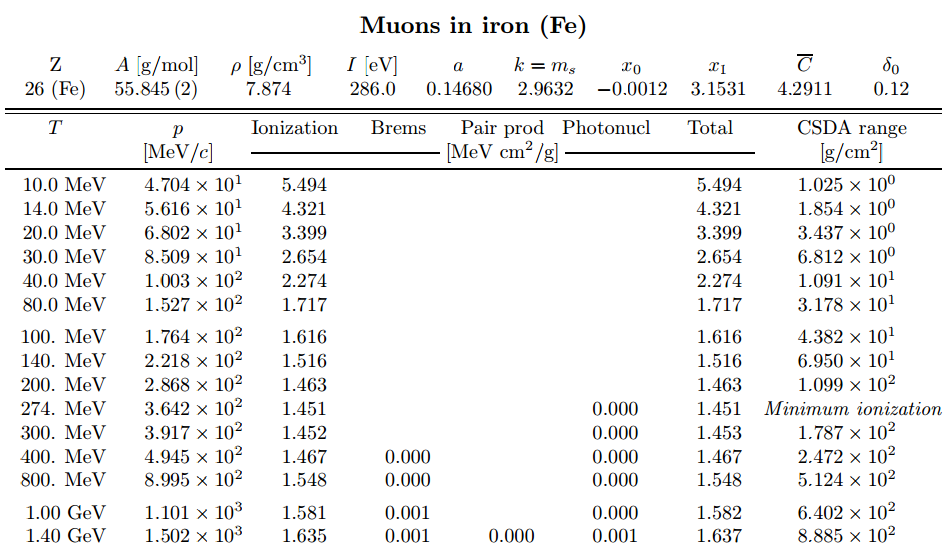
\includegraphics[width=\textwidth]{Figures/E_loss_Fe} 
  \caption{Energy loss table for muons in iron. Table courtesy of \cite{PDGTables}.}
  \label{fig:elossfe}
\end{figure}

This is a good example because all of the cooling materials currently being considered have less muon stopping power than iron. This means that iron represents the maximum contribution of non-ionization energy loss per initial beam energy; that is, the non-ionization effects begin to emerge at much higher energies for lighter elements such as liquid hydrogen. Note that Figure \ref{fig:bethecurve} may also be useful when discussing this subject.

Here, \textit{ionization} refers to both true ionization (the production of $\delta$ rays) and excitation (the promotion of an inner electron to a higher shell). To reiterate a previous section, the term `straggling' refers to the fluctuation about some mean energy loss. That is to say, the amount of energy that a particle will lose is intrinsically random --there exists some distribution with some average value, and when the particle of interest transverses a length of matter the amount of energy that this particle loses is selected from this distribution. This intrinsic randomness can be attributed to quantum-like behaviors (e.g. the energy loss cross section which comes from the wave nature of the particle in question).
}
\Chapter{Stochastic Processes in Other Codes} \label{chp:other_codes}
In this chapter, the two major stochastic processes---energy straggling and multiple scattering---are detailed. Because there are so many models for these two key processes, two case studies will be shown as a frame for their derivations. Both of these codes use particle-by-particle propagation and do not use the transfer map method discussed in Section \ref{sec:cosy}.

The first case study is ICOOL \cite{icool} and will cover the classic models. Much of the classic theory is also used in the new COSY routines. Consequently, the sections concerning ICOOL serve as a foundation for the derivations in Chapter \ref{chp:cosy}. ICOOL was created at Brookhaven National Laboratory for the benefit of the members of the Neutrino Factory and Muon Collider Collaboration, who specifically study ionization cooling problems.

The second case study is G4Beamline \cite{g4bl}, which is based on GEANT4 \cite{geant4}. GEANT4 implements a more novel approach. Many of the routines use empirically-tuned parameters. Consequently, G4Beamline is accurate for a variety of particles over a wide range of energies. It should be noted that muons, for which thet is little experimental data available, are usually grouped with protons as heavy charged particles. Therefore, for lack of experimental data, muons use the same routines as protons.

\Section{Energy Straggling in ICOOL} \label{sec:ICOOLStraggling}\par
ICOOL \cite{icool} employs four straggling models, three of which were used in these muon simulations studies. Discussed below, these are
\begin{enumerate}
\item{Gaussian (Bohr)},
\item{Landau distribution}, and
\item{Vavilov distribution (with appropriate limits)}.
\end{enumerate}
The fourth model was not considered for this study.

\Subsection{Gaussian (Bohr) Straggling Model} \label{ssc:ICOOLStragglingGaussian}
The first model uses a Guassian function to model the energy loss distribution. Recall that Gaussian distributions are defined by two parameters: the standard deviation $\sigma$ and the mean $\mu$. 

According to \cite{geant4}, the first of these is given by:
\begin{equation}\label{eqn:bohrvariance}
\sigma^2=2\pi e^2 N_A T_c \frac{Z\rho L}{A} \frac{1-\beta^2/2}{\beta},
\end{equation}
where $e$ is the fundamental electric charge, $N_A$ is Avagadro's number, $T_c$ is the cut kinetic energy of $\delta$-electrons, $Z$ is the nuclear charge, $\rho$ is the density of the material, $L$ is the length of the material, $A$ is the nuclear mass, and $\beta=v/c$ is the relativistic speed.

The mean comes from the Bethe-Bloch equation \cite{bethebloch}, which will be derived here and yeilds Eqn. \ref{eqn:bethebloch}. The derivation is the so-called classical derivation, which takes first principles and mechanically derives an expression. The classically-derived intermediate equation is then subject to modern corrections, which account for the approximations made or phenomena neglected during the classical derivation.

%..........................................
%\vspace{24pt}
\noindent \textit{\large Classical Derivation}
%\vspace{12pt}

The process begins with a particle of charge $e$ moving through a material. It is assumed that the mass of the incoming particle is much greater than the mass of the electron since scattering will be neglected in this derivation. Moreover, the electron must either be at rest and fixed into place (which is nonphysical) or the collision time of the particle and electron must be very small compared to the electron orbital time. The longitudinal ($z$) axis is aligned with the particle velocity such that $v_x=v_y=0$. The momentum transfer $\Delta p$ from the incoming particle to the orbiting electron is sought via
\begin{align*}
\Delta p =  \int_{-\infty} ^\infty F dt.
\end{align*}

The first observation is that the change in the longitidunal force on the particle is zero. This is true since the particle feels an average force ``forward'' just as much as it feels a force ``backward'' due to symmetry. Explicitly, this is equivalent to saying that $F_z(z)=-F_z(-z)$.
\iffalse




Explicitly, using Figure \ref{fig:bethe_bloch} as a reference it can be seen that
\begin{align*}
\Delta p_z &= \int_{-\infty} ^\infty F_z dt = \int_{-\infty} ^\infty F \sin\theta \frac{dz}{v} = \int_{-\infty} ^\infty \frac{e^2}{r^2} \frac{z}{r} \frac{dz}{v}=\frac{e^2}{v} \int_{-\infty} ^\infty \frac{z}{r^3}dz,
\end{align*}
where $F$ is the electrostatic force ($e^2/r^2$) between the particle and the stationary electron, $r$ is the distance between the particle and the electron, and $v$ is the particle's velocity. Using
\begin{align*}
r=\sqrt{z^2+b^2},
\end{align*}
where $b$ is the impact parameter (the closest distance between the particle and the electron), then
\begin{align*}
\Delta p_z = \frac{e^2}{v} \int_{-\infty} ^\infty \frac{z}{(z^2+b^2)^{3/2}}dz = 0.
\end{align*}


\fi
For this reason, any change in momentum is solely due to the transverse force. Again following Figure \ref{fig:bethe_bloch},
\begin{align*}
\Delta p &=\int_{-\infty} ^\infty F_x \ dt = \int_{-\infty} ^{\infty} F_x \frac{dz}{v} = \int_{-\infty} ^{\infty} F\cos{\theta}\frac{dz}{v},
\end{align*}
 Observe from Figure \ref{fig:bethe_bloch} that $\cos\theta = b/r$. Then
\begin{align*}
\Delta p &= \int_{-\infty} ^{\infty} \frac{e^2}{r^2} \frac{b}{r} \frac{dz}{v} = \int_{-\infty} ^{\infty} \frac{e^2}{z^2+b^2} \frac{b}{\sqrt{z^2+b^2}} \frac{dz}{v}\\
\Delta p &= \frac{e^2 b}{v} \int_{-\infty} ^{\infty} \frac{1}{(z^2+b^2)^{3/2}}dz.
\end{align*}
By substitution of the following
\begin{align*}
z = b\tan{\theta},&\qquad dz = b\sec^2{\theta} d\theta,\\
z=-\infty\rightarrow \theta = \frac{-\pi}{2},&\qquad z=\infty \rightarrow \theta = \frac{\pi}{2}.
\end{align*}
the integral becomes
\begin{align*}
\Delta p &=\frac{e^2 b}{v}\int_{-\pi/2} ^{\pi/2} \frac{b\sec^2{\theta} d\theta}{(b^2(\tan^2{\theta}+1))^{3/2}} =\frac{e^2 b}{v}\int_{-\pi/2} ^{\pi/2} \frac{d\theta}{b^2 |\sec{\theta}|}\\
\Delta p&=\frac{2e^2}{vb}.
\end{align*}

\begin{figure}[h!]
  \centering
    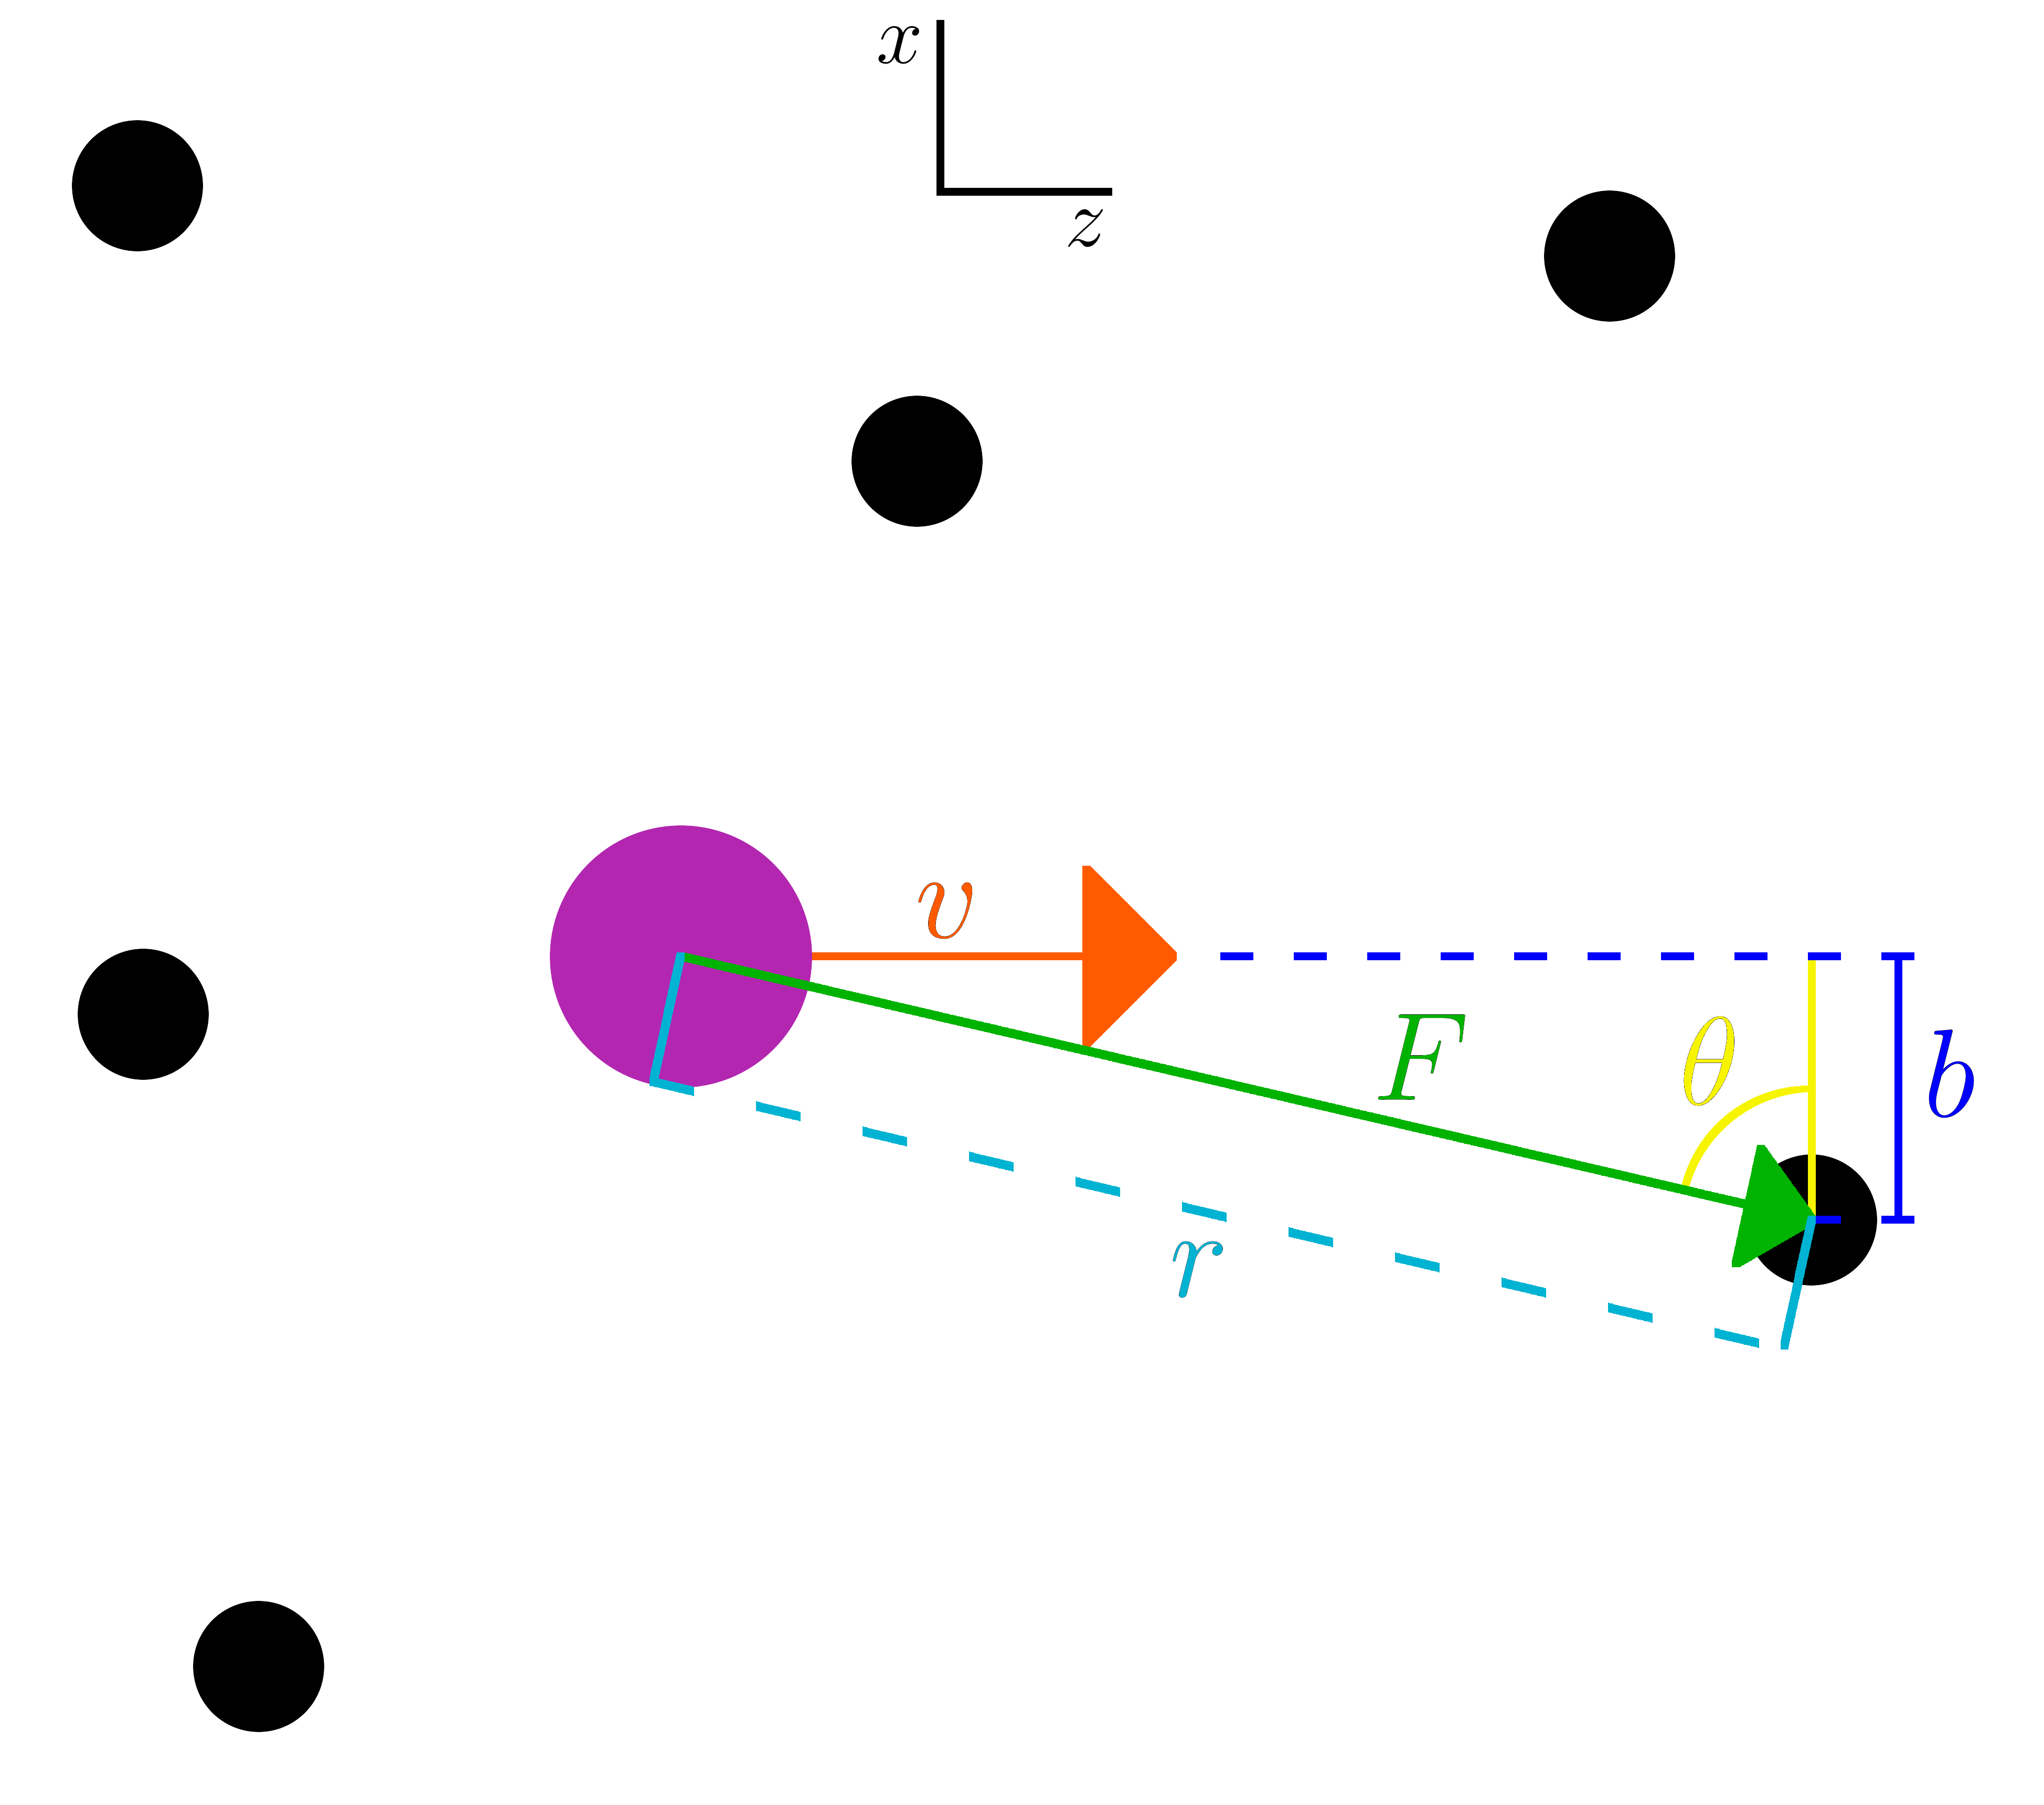
\includegraphics[width=0.7\textwidth]{Figures/bethe_bloch} 
  \caption{Classical model of particle passage through matter.}
  \label{fig:bethe_bloch}
\end{figure}

The non-relativistic approach yeilds the energy loss for the interaction between a muon and a single bound electron:
\begin{equation}\label{eqn:BetheBlochDeltaE}
\epsilon=\frac{\Delta p^2}{2m_e}=\frac{2e^4}{v^2 b^2 m_e}.
\end{equation}

Here, it is useful to note that if the interaction of the muon with the nucleus was desired, $\epsilon$ for a single interaction would be proportional to $Z^2/m_{nuc}$ and would be added on to Eqn. \ref{eqn:BetheBlochDeltaE}. However, since $1/m_e \gg 1/m_{nuc}$ the second term will be disregarded.

Observe from Figure \ref{fig:bethe_bloch} that only a single electron has been considered for Eqn. \ref{eqn:BetheBlochDeltaE}. For multiple electrons, the average electron density is $N_{el}=N_A\cdot Z\rho/A$, where $N_A$ is Avagadro's number, $Z$ is the nuclear charge, $\rho$ is the density of the material, and $A$ is the nuclear mass. From this expression the average energy loss may be obtained. The cylindrical symmetry of the system is exploited by integrating the single electron interaction in cylidrical coordinates, with $\theta$ as the cylindrical angle, $b$ (the impact parameter) as radius, and $z$ as length. The bounds are $\theta \in [0,2\pi]$, $z\in[0,L]$ (where $L$ is the total length of material traversed), and $b\in[b_{min},b_{max}]$ (which will be discussed shortly). Then
\begin{align}
\left<\epsilon\right>&=\int_{b_{min}} ^{b_{max}} \int_0 ^L \int_0 ^{2\pi}  \frac{2e^4}{v^2b^2m_e}N_{el}\: d\theta \: dz\: b \,db \nonumber\\
&=\frac{4\pi N_A e^4}{v^2 m_e}\frac{Z\rho L}{A}\int_{b_{min}} ^{b_{max}} \frac{db}{b}. \label{eqn:BetheBlochIntermediate}
\end{align}

It is known that $b_{min}$ comes from the maximum amount of energy ($T_{max}$) which a muon may impart upon an electron. This quantity is derived later and can be seen in Eqn. \ref{eqn:tmax}, but is only symbolic here. Similarly, the minimum transferrable energy will be taken as the mean ionization energy, $I$, which is usually an empirical value. Any energy below this value will not transfer, since this is the minimum amount of energy to free the electron from its orbit. Then
\begin{align*}
\epsilon_{max}&=\frac{2e^4}{v^2b_{min} ^2 m_e}=T_{max},\\
b_{min}&=\frac{e^2}{v}\sqrt{\frac{2}{m_e T_{max}}},\\[12pt]
\epsilon_{min}&=\frac{2e^4}{v^2b_{max} ^2 m_e}=T_{min}=I,\\
b_{max}&=\frac{e^2}{v}\sqrt{\frac{2}{m_e I}}.
\end{align*}

Once the bounds have been acquired, the integral in Eqn. \ref{eqn:BetheBlochIntermediate} is solvable.
\begin{align}
\left<\epsilon\right> &= \frac{4\pi N_A e^4}{v^2 m_e} \frac{Z\rho L}{A}\int_{b_{min}} ^{b_{max}} \frac{db}{b},\nonumber\\
\left<\epsilon\right> &= \frac{4\pi N_A e^4}{v^2 m_e} \frac{Z\rho L}{A} \ln{\frac{b_{max}}{b_{min}}},\nonumber\\
\left<\epsilon\right> &= \frac{2\pi N_A e^4}{v^2 m_e} \frac{Z\rho L}{A} \ln{\frac{T_{max}}{I}} \label{eqn:BetheBlochClassical}.
\end{align}

\noindent \textit{\large{Modern Corrections}}

\iffalse
While Eqn. \ref{eqn:BetheBlochClassical} is a good start, there are many aspects which were not considered. The most obvious of these are the wavelike nature of the incoming muon, relativistic kinetic energy (not simply $p^2/2m$), and the relativistic flattening of the muon's electric field just to name a few. Therefore, a more rigorous derivation will be done with corrections added onto it.

Firstly, let the incoming muon be considered also a wave. Then the corresponding differential cross section $d\Sigma$ is defined as the area in which the muon loses an amount of energy between $\epsilon$ and $\epsilon+d\epsilon$. Given the impact parameter $b$, for a single electron this area is a ring of radius $b$ and thickness $db$, or \cite{bichsel1968,bichsel1988}
\begin{align*}
d\Sigma=2\pi b \, db.
\end{align*}
Using the result from Eqn. \ref{eqn:BetheBlochDeltaE} in the classical derivation, this becomes
\begin{align*}
\epsilon &= \frac{2e^4}{\beta^2 b^2 m_e}\\
b^2 &= \frac{2e^4}{\beta^2 \epsilon m_e}\\
2b \, db &= -\frac{2e^4}{\beta^2 \epsilon^2 m_e}d\epsilon,
\end{align*}
and so
\begin{align*}
d\Sigma=\frac{2\pi e^4}{\beta^2} \frac{d\epsilon}{\epsilon ^2}.
\end{align*}
The relativistic correction for this was calculated by Bhabha \cite{uehling,bhabha} and results in
\begin{align*}
d\Sigma=\frac{2\pi e^4}{\beta^2} \frac{d\epsilon}{\epsilon ^2}\Big(1-\frac{\beta^2 \epsilon}{T_{max}}\Big).
\end{align*}
Note that in \cite{uehling}, this result is only for spin-0 particles, and there is a further correction factor of $\epsilon ^2 / 2E^2$ for spin-1/2 particles. However, since $E>>\epsilon$ this term is usually ignored.

The cross section may now be used in the standard definition of moments (or expectation values). Then
\begin{align} \label{eqn:StragglingMoments}
\left< M^j\right>&=N_{el} L \int_{\epsilon_{min}} ^{\epsilon_{max}} \epsilon^j \frac{d\Sigma}{d\epsilon} d\epsilon .
\end{align}
The moments are simply equal to the expectation values as $M^j=\left<\epsilon ^j \right>$, except for $M^0$, since $\left< \epsilon ^0 \right>=\left< 1 \right> = 1$. Instead, $M^0$ is the mean number of collisions, and the actual number of collisions is sampled from a Poisson distribution with this average.

While the upper limit $\epsilon_{max}$ is still valid since it was derived explicitly from relativistic principles, the lower limit $\epsilon_{min}$ should be re-evaluated from its classical assumption. \cite{bichsel1968} points out that the incoming particle interacts with all of the electrons in the atom, not simply a single valence electron. These interactions may be significant enough to invalidate the classical model and therefore should be considered. $I$ is defined as (see for example Eqns. \ref{eqn:G4StragglingOscillatorConstraint1} and \ref{eqn:G4StragglingOscillatorConstraint2} in Section \ref{sec:g4blstraggling})
\begin{gather*}
Z \ln I = \sum_i f_i E_i
\end{gather*}
where $f_i$ are oscillator strengths and $E_i$ are ionization energies for the $i^{th}$ level.
\fi

\iffalse
It is interesting to note that the zeroth moment is the mean number of collisions, and that the actual number of collisions is sampled from a Poisson distribution with this average. Moreover, $\left<\epsilon^1\right>$ is the mean energy loss, which is the desired outcome of this derivation. Then
\begin{align*}
\left<\epsilon\right>&=\frac{Z\rho L}{A} \frac{2\pi e^4}{\beta^2} \int_I ^{T_{max}} \frac{d\epsilon}{\epsilon} \Big(1-\frac{\beta^2 \epsilon}{T_{max}}\Big)\\
\left<\epsilon\right>&=\frac{Z\rho L}{A} \frac{2\pi e^4}{\beta^2} \Big(\ln{\frac{T_{max}}{I}}-\beta^2 (1-\frac{I}{T_{max}})\Big)
\end{align*}
\fi





There are a number of corrections to the Bethe-Bloch equation. The first is a correction under the logarithm due to the relativistic flattening of the incoming particle's electric field. This factor is  $2m_e \beta^2 \gamma^2 / I$. Another correction is known as the density correction $\delta$ and arises due to polarization of the material. This is important for high energies since it can limit the range of the flattened electric field in the material. The last correction is the shell correction $C$ and accounts for the fact that the electron is not at rest (or the interaction time is not much faster than the electron orbit). This is important for low energies. These corrections may or may not have a large impact on these medium energy studies, since the logarithmic and density corrections arise at high energies and the shell correction occurs at low energies. Finally, in its more familiar form, the constants in Eqn. \ref{eqn:BetheBlochClassical} are condensed into a single constant $K=\frac{2\pi e^4 N_A}{m_e}\approx 15.4$ $ (\text{MeV}\cdot \text{cm}^3)/(\text{m}\cdot \text{g})$. Since the model assumes natural units (i.e. $c=1$), $v^2$ is usually replaced with $\beta ^2$. Moreover, to avoid confusion $\left<\epsilon\right>$ is given a negative sign in order to emphasize energy \emph{loss}.

The ultimate result is the Bethe-Bloch equation for the average energy lost by a particle traversing some medium with correction factors:
\begin{equation}\label{eqn:bethebloch}
\left< \epsilon \right> = -\frac{K}{\beta^2}\frac{Z\rho L}{A}\Big(\ln{\frac{2m_e \beta ^2 \gamma ^2 T_{max}}{I^2}}-2\beta^2-\delta-2\frac{C}{Z}\Big).
\end{equation}

According to the Particle Data Group \cite{PDG}, this equation is generally accurate for intermediate $Z$ materials (up to a few \% when compared to experimental data) in the energy regime of $0.1 \lesssim \beta \gamma \lesssim 1000$. The lower limit of this equation is reached when the incoming particle velocity is comparable to the atomic electron velocities and the upper limit is attained due to radiative effects, and both limits exhibit some $Z$ dependence. Figure \ref{fig:bethecurve} depicts this region with muons on copper. Clearly, the region typically used for muon ionization cooling ($100 \text{ MeV/}c < p_\mu < 1000 \text{ MeV/}c$) falls in the middle of the Bethe region.

%..........................................
\vspace{24pt}
\noindent \textit{\large{Derivation of $\,T_{max}$}}
\vspace{12pt}

Although $T_{max}$ is used symbolically in many equations, here it will be derived explicitly from a relativistic point of view. This derivation yields Eqn. \ref{eqn:tmax} and works in natural units such that $c=1$. Conservation of energy for a muon incident upon an electron at rest requires that 
\begin{align}
E_\mu+m_e&=E_{\mu,f}+E_e,&\text{ or} \nonumber\\
\sqrt{p_\mu ^2+m_\mu ^2}+m_e &= \sqrt{p_{\mu,f}^2+m_\mu ^2}+T_e+m_e,&\text{ or} \nonumber \\
p_{\mu,f}^2 =p_\mu^2 &+T_e^2-2T_e\sqrt{p_\mu ^2 + m_\mu^2}, \label{eqn:TMaxEnergy1}
\end{align}
with
\begin{align}
E_e=T_e&+m_e = \sqrt{p_e ^2+m_e^2},\qquad\text{ or} \nonumber\\
p_e ^2&=(T_e+m_e)^2-m_e^2, \label{eqn:TMaxEnergy2}
\end{align}
where $T_e$ is the final kinetic energy of the electron, $p_\mu$ is the initial muon momentum, $m_\mu$ is the mass of the muon, and $p_{\mu,f}$ is the final muon momentum. 

Conservation of momentum requires that
\begin{align*}
\vec{p}_\mu&=\vec{p}_{\mu,f}+\vec{p}_e, \qquad\text{ or}\\
 p_{\mu,f}^2&=p_\mu ^2 + p_e^2-2p_\mu p_e \cos\alpha,
\end{align*}
where $\alpha$ is the angle between the initial muon momentum and the final electron momentum.
Using Eqn. \ref{eqn:TMaxEnergy2} for $p_e$ on the right-hand side this becomes
\begin{align*}
p_{\mu,f}^2=p_\mu ^2+(T_e+m_e)^2-m_e ^2-2p_\mu\cos\theta \sqrt{(T_e+m_e)^2-m_e^2}.
\end{align*}
Now subsitution of Eqn. \ref{eqn:TMaxEnergy1} for $p_{\mu,f} ^2$ on the left-hand side yields
\begin{align*}
p_\mu ^2+T_e ^2 - 2T_e \sqrt{p_\mu^2+m_\mu ^2}&=p_\mu ^2+(T_e+m_e)^2-m_e ^2 -2p_\mu\cos\theta\sqrt{(T_e+m_e)^2-m_e^2}.
\end{align*}
For maximum energy (i.e. to attain $T_e=T_{max}$), $\cos\theta=1$, which is representative of a head-on collision. Then
\begin{align*}
T_{max} ^2-2T_{max}\sqrt{p_\mu ^2+m_\mu ^2} &=T_{max}^2+2T_{max}m_e-2p_\mu\sqrt{T_{max}^2+2T_{max}m_e}\\
-2T_{max}(\sqrt{p_\mu ^2 + m_\mu ^2}+m_e)&=-2p_\mu\sqrt{T_{max}^2+2T_{max}m_e}\\
\sqrt{p_\mu ^2+m_\mu ^2}+m_e&=p_\mu\sqrt{1+\frac{2m_e}{T_{max}}}.
\end{align*}
Substituting the initial muon energy $E_\mu=\sqrt{p_\mu ^2+m_\mu ^2}=\gamma m_\mu$ and the initial muon momentum $p_\mu ^2=E_\mu ^2 - m_\mu ^2 = m_\mu ^2 (\gamma^2-1)=m_\mu ^2 \gamma^2 \beta^2$ results in
\begin{align*}
\gamma m_\mu + m_e &= m_\mu\gamma\beta\sqrt{1+\frac{2m_e}{T_{max}}}\\
(\gamma m_\mu +m_e)^2 &=m_\mu^2\gamma^2\beta^2 \Big(1+\frac{2m_e}{T_{max}}\Big).
\end{align*}
Finally, solving for the maximum transferrable energy from an incident muon to an electron at rest is
\begin{equation}\label{eqn:tmax}
T_{max}=\frac{2m_e \beta^2 \gamma^2}{1+2\gamma\frac{m_e}{m_\mu}+(\frac{m_e}{m_\mu})^2}.
\end{equation}

%-----------------------------------------------------------------------------------------------------------
\Subsection{Landau Straggling Model}\label{ssc:ICOOLStragglingLandau}

The second ICOOL straggling model selects an energy loss from a Landau distribution \cite{landau}. This derivation is particularly important since it is the same model that was implemented into COSY in this work. Landau begins the derivation by stipulating that this theory assumes fast particles (``so that the usual ionisation theory may be applied'', here taken as particles whose energy is in the Bethe regime in Figure \ref{fig:bethecurve}). Moreover, the thickness of the absorber should be small enough, so that the energy loss is small compared to the initial energy. Landau defines the weight function $w(E,u)$ as the probability per unit length of an energy loss $u$ given the instantaneous total energy $E$. For the aforementioned constraints, the weight function may be written simply as $w(u)$ (since $E$ is now a constant instead of a variable). Another way of describing this constraint is that the total energy of the particle is roughly constant while traversing the medium.

Let $f(L,\epsilon)$ be the desired distribution function for the energy loss. This means that the particle will lose an amount of energy between $\epsilon$ and $\epsilon+d\epsilon$ while traversing an absorber of length $L$. Then on one hand
\begin{align*}
\text{change in $f$ per unit length }=\frac{\partial f(L,\epsilon)}{\partial L}.
\end{align*}
On the other hand, the change in $f$ may also be expressed as the difference of two functions: one at a length $L$ with possible energy losses between $\epsilon$ and $\epsilon+d\epsilon$ and another at length $L$ and with possible energy losses between $\epsilon-u$ and $\epsilon+d\epsilon-u$, with $u$ accounting for the infinitesimal change in length. Then
\begin{align*}
\text{change in $f$ per unit length }=\Bigg [\int_0 ^\infty w(u) f(L,\epsilon-u) du \Bigg] - f(L,\epsilon).
\end{align*}
Often referred to as the integral transport equation, the two previous definitions of the change in $f$ per unit length may be combined as
\begin{align}\label{eqn:Landau1}
\frac{\partial f(L,\epsilon)}{\partial L} = \Bigg [\int_0 ^\infty w(u) f(L,\epsilon-u) du \Bigg] - f(L,\epsilon).
\end{align}
Since $L$ and $\epsilon$ are independent and implicit variables, this allows for a Laplace transformation. Take the transformed function with respect to $\epsilon$ as 
\begin{align*}
\phi(p,L)=\int_0 ^\infty e^{-p \epsilon} f(\epsilon) d\epsilon.
\end{align*}
(Note that $p$ is simply a dummy variable and not the momentum.)
%
Then the inverse transformation gives
\begin{align} \label{eqn:LandauInverseTransformation}
f(L,\epsilon)=\frac{1}{2\pi i} \int_{K-i \infty} ^{K+i\infty} \phi(p,L) e^{p\epsilon} dp.
\end{align}
Observe here that $K>0$ and so the integral is just to the right of the imaginary axis. This is the desired distribution function, and so will be useful later. However, without the form of $\phi$ it is not useful. The goal then will be to find a closed form of $\phi$.

Multiplying both sides of Eqn. \ref{eqn:Landau1} by $e^{-p\epsilon}$ and integrating with respect to $d\epsilon$ yields
\begin{align*}
\int_0 ^\infty \frac{\partial f}{\partial L} e^{-p\epsilon} d\epsilon = \int_0 ^\infty \Bigg [\int_0 ^\infty w(u) f(L,\epsilon-u) du \Bigg]e^{-p\epsilon} d\epsilon -  \int_0 ^\infty f(L,\epsilon) e^{-p\epsilon} d\epsilon.
\end{align*}
On the left side, the operations of partial derivative and integration are commutable, and are therefore switched. On the right side, the first term has commutable integrations and so the order is switched. For the second term, note that $w(u)$ is normalized, so adding the integral of $w(u)$ over all $u$ changes nothing. Dropping the implicit $L$ for now,
\begin{align*}
\frac{\partial}{\partial L}\int_0 ^\infty e^{-p\epsilon} f(\epsilon) d\epsilon = &\int_0 ^\infty \Bigg[\int_0 ^\infty e^{-p\epsilon} f(\epsilon-u)  d\epsilon \Bigg] w(u) du -\\
 & \int_0 ^\infty \Bigg[\int_0 ^\infty e^{-p\epsilon}f(\epsilon) d\epsilon \Bigg] w(u) du.
\end{align*}
Parts of the left side and the second term on the right side may be substituted for $\phi$ directly, while the first term on the right side should be shifted by $-u$, resulting in
\begin{align*}
\frac{\partial}{\partial L} \phi(p,L) &= \int_0 ^\infty \Bigg[\int_{-u} ^\infty e^{-p(\epsilon+u)} f(\epsilon)  d\epsilon \Bigg] w(u) du -\int_0 ^\infty \phi(p,L) w(u) du.
\end{align*}
Now recall that $f(\epsilon)$ is the desired function for energy loss. Therefore, $f(\epsilon<0)=0$ (i.e. the particle cannot gain energy while traversing a medium), and so
\begin{align}
\frac{\partial}{\partial L} \phi(p,L) &= \int_0 ^\infty e^{-pu}\Bigg[\int_{0} ^\infty e^{-p\epsilon} f(\epsilon)  d\epsilon \Bigg] w(u) du -\phi(p,L) \int_0 ^\infty w(u) du\nonumber\\
&=\phi(p,L)\int_0 ^\infty w(u)(e^{-pu}-1)\, du. \nonumber%\label{eqn:LandauPhiDifferentialEquation}
\end{align}

This differential equation is a first-order, undriven normal linear ODE (ordinary differential equation) \cite{Borrelli}. Let prime ( $'$ ) denote a partial derivative with respect to $L$. Then the strategy to solve this ODE is to define a function $h(L)$ as
%
\begin{gather*}
h(L)=-\int_0 ^\infty w(u)  (e^{-pu}-1)\, du
\end{gather*}
and its antiderivative as
\begin{gather*}
H(L)=\int h(L) dL=L \int_0 ^\infty w(u)  (1-e^{-pu})\, du.
\end{gather*}
Then
\begin{equation}\label{eqn:landauODE}
\phi ' + \phi \cdot h(L) = 0.
\end{equation}
%
Since $(e^{H(L)}) ' = e^{H(L)}\cdot H'(L)= e^{H(L)}\cdot h(L)$ , it is useful to multiply both sides of the ODE in Eqn. \ref{eqn:landauODE} by $e^{H(L)}$, resulting in
\begin{gather*}
\phi ' \cdot e^{H(L)}+ \phi \cdot h(L) \cdot e^{H(L)} = 0,\\
(\phi\cdot e^{H(L)}) ' = 0.
\end{gather*}
Integrating both sides yields
\begin{gather*}
\phi\cdot e^{H(L)}=K_1,\\
\phi = K_1 e^{-H(L)},\\
\phi(p,L)=K_1 \exp\Big[-L\int_0 ^\infty w(u)  (1-e^{-pu})\, du\Big].
\end{gather*}

This differential equation is now solvable provided that there are initial conditions. The first observation is that for $L=0$, the only possible energy loss is zero. Mathematically, this means that $f(0,\epsilon)=\delta(\epsilon)$; that is, the probability of energy loss is 100\% for an energy loss of zero and 0\% for all other energy losses. Then the boundary condition on $\phi$ is
\begin{align}
\phi(p,0)&=\int_0 ^\infty \delta(\epsilon) e^{-p\epsilon}\, d\epsilon\nonumber\\
\phi(p,0)&=e^{p\cdot 0}\nonumber\\
\phi(p,0)&=1=K_1\exp[0].\nonumber%\label{eqn:LandauPhiInitialCondition}
\end{align}
Then
\begin{gather*}
\phi(p,L)=\exp\Big[-L\int_0 ^\infty w(u)  (1-e^{-pu})\, du\Big].
\end{gather*}

Now using Eqn. \ref{eqn:LandauInverseTransformation}, the energy loss distribution function $f$ in terms of $w(u)$ is 
\begin{equation} \label{eqn:LandauGeneralSolution}
f(L,\epsilon)=\frac{1}{2\pi i} \int_{K-i\infty} ^{K+i\infty} \exp\Big[p\epsilon-L\int_0 ^\infty w(u)  (1-e^{-pu})\, du\Big] dp.
\end{equation}
In principle, this is the general solution to the energy loss profile for a particle traversing some medium. In practice, the only thing which is inhibiting implementation is an algorithm to generate a number from this distribution (which will be discussed in Chapter \ref{chp:cosy}) and the function $w(u)$. Once $w(u)$ is obtained, the integral may be found using numeric integration, provided that it is not computationally expensive.

Livingston and Bethe \cite{livingston} derived the form of $w(u)$ in 1937, and it is
\begin{align*}
w(u)&=\frac{\xi}{L}\frac{1}{u^2},
\end{align*}
where
\begin{equation}\label{eqn:xi}
\xi=\frac{2\pi r_e ^2 m_e N_A Z\rho L}{\beta^2 A}
\end{equation}
and $r_e$ is the classical electron radius, $m_e$ is the electron mass, $N_A$ is Avagadro's number, $Z$ is the nuclear charge, $\rho$ is the density of the material, $L$ is the length of the material, $A$ is the nuclear mass, and $\beta=v/c$ is the relativistic speed. Now the form of $w(u)(1-e^{-pu})$ may be seen in Figure \ref{fig:landauPUPlot}. It can be seen that the most important values of $p$ are those where $pu \ll 1$ and $1 \ll pu$ since values of $pu\approx 1$ will tend to vanish.

\begin{figure}[h!]
  \centering
    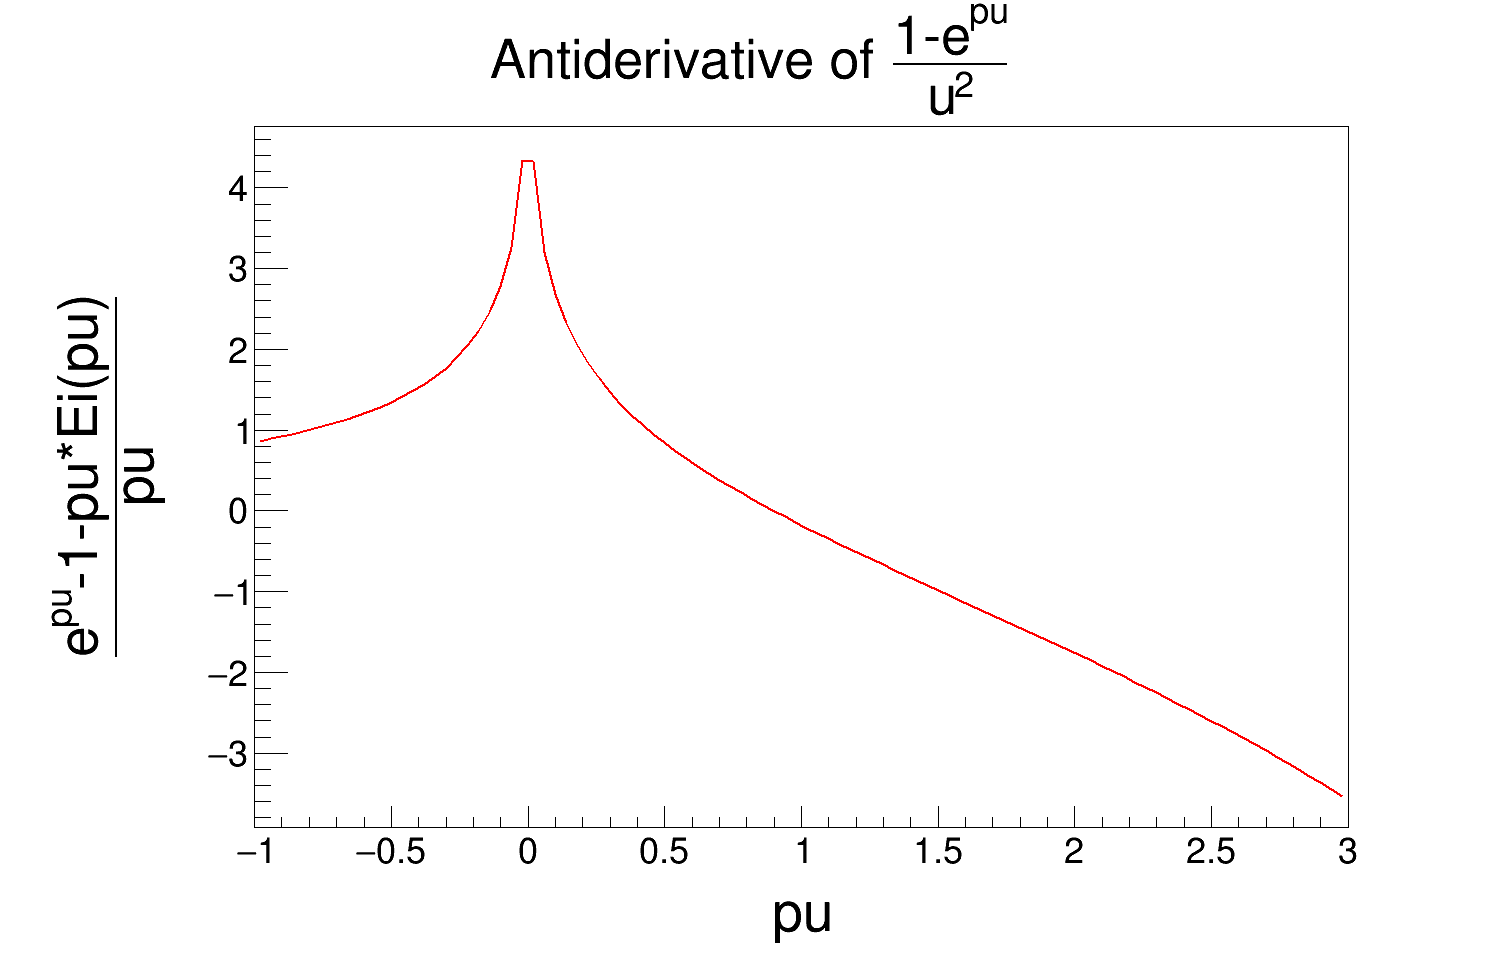
\includegraphics[width=0.7\textwidth]{Figures/landauPUPlot} 
  \caption[Plot of $\int w(u)(1-e^{-pu})\ du$.]{Plot of $\int w(u)(1-e^{-pu})\ du$ for various $pu$. On the vertical axis is the antiderivative of $w(u)(1-e^{-pu})$, with $\text{Ei}(x)$ representing the exponential integral.}
  \label{fig:landauPUPlot}
\end{figure}

Rather than zero, let $u_{min}$ be the minimum possible energy loss. Now consider a certain energy $u_1$ such that $u_{min}\ll u_1$ and $pu_1 \ll 1$. Then the integral in the exponent of Eqn. \ref{eqn:LandauGeneralSolution} has the form
\begin{align*}
L\int_0 ^\infty w(u)  (1-e^{-pu})\, du &= \xi\Big( \int_0 ^{u_1} \frac{1-e^{-pu}}{u^2} du + \int_{u_1} ^\infty \frac{1-e^{-pu}}{u^2} du\Big) .
\end{align*}
Since the first integral is over the small values, it is possible to write $1-e^{pu} \approx 1-(1-pu) = pu$. Furthermore, the minimum energy loss is not 0 but rather $u_{min}$. Then
\begin{align*}
\frac{L}{\xi}\int_0 ^\infty w(u)  (1-e^{-pu})\, du &=\int_{u_{min}} ^{u_1} \frac{p\ u}{u^2} du + \int_{u_1} ^\infty \frac{1-e^{-pu}}{u^2} du\\
&=p\int_{u_{min}} ^{u_1} \frac{1}{u} du + \int_{u_1} ^\infty \frac{1-e^{-pu}}{u^2} du\\
&=p \ln\frac{u_1}{u_{min}} + \int_{u_1} ^\infty \frac{1-e^{-pu}}{u^2} du.
\end{align*}
For the second term, integration by parts and evaluation at the boundaries gives
\begin{align*}
\frac{L}{\xi}\int_0 ^\infty w(u)  (1-e^{-pu})\, du &=p \ln\frac{u_1}{u_{min}} + \frac{1-e^{-pu_1}}{u_1}+p\int_{u_1}^\infty \frac{e^{-pu}}{u} du.
\end{align*}
Recalling that $u_1$ was chosen such that $pu_1 \ll 1$, the exponential in the second term may be approximated as $e^{-pu_1}\approx 1-pu_1$. Then
\begin{equation} \label{eqn:landauIntermediate1}
\frac{L}{\xi}\int_0 ^\infty w(u)  (1-e^{-pu})\, du =p \ln\frac{u_1}{u_{min}} + p+p\int_{u_1}^\infty \frac{e^{-pu}}{u} du.
\end{equation}
The final integral may be evaluated first by letting $K_2=pu$:
\begin{align*}
\frac{L}{\xi}\int_{u_1}^\infty \frac{e^{-pu}}{u} du &= \int _{pu_1} ^\infty \frac{e^{-K_2}}{K_2}dK_2\\
&= \int_{pu_1} ^\infty \frac{e^{-K_2}}{K_2} dK_2 + \int_{pu_1} ^1 \frac{dK_2}{K_2} - \int_{pu_1} ^1 \frac{dK_2}{K_2} \\
&= \int_{pu_1} ^1 \frac{e^{-K_2}}{K_2} dK_2 + \int_1 ^\infty \frac{e^{-K_2}}{K_2} dK_2 + \int_{pu_1} ^1 \frac{dK_2}{K_2} - \int_{pu_1} ^1 \frac{dK_2}{K_2} \\
&= \int_{pu_1} ^1 \Big(\frac{e^{-K_2}}{K_2}-\frac{1}{K_2}\Big) dK_2 + \int_1 ^\infty \frac{e^{-K_2}}{K_2} dK_2 + \int_{pu_1} ^1 \frac{dK_2}{K_2} \\
&= \int_{pu_1} ^1 \frac{dK_2}{K_2} + \left[\int_{pu_1} ^1 \frac{e^{-K_2}-1}{K_2} dK_2 + \int_1 ^\infty \frac{e^{-K_2}}{K_2} dK_2 \right].
\end{align*}
The first term is easily evaluated, and the second term in brackets is approximately\footnote{This expression would be exactly $-C_{Euler}$ if $pu_1=0$.} the negative of Euler's constant, $-C_{Euler}$. Putting this back into Eqn. \ref{eqn:landauIntermediate1} yields
\begin{align*}
\frac{L}{\xi}\int_0 ^\infty w(u)  (1-e^{-pu})\, du &=p \ln\frac{u_1}{u_{min}} + p(1-C_{Euler}-\ln pu_1)\\
&=p(1-C_{Euler}-\ln pu_{min}).
\end{align*}

Now Eqn. \ref{eqn:LandauGeneralSolution} may be rewritten as
\begin{align*}
f(L,\epsilon)&=\frac{1}{2\pi i} \int_{K-i\infty} ^{K+i\infty} \exp\Big[p\epsilon-L\int_0 ^\infty w(u)  (1-e^{-pu})\, du\Big] dp\\
&= \frac{1}{2\pi i} \int_{K-i\infty} ^{K+i\infty} \exp\Big[p\epsilon-p\xi(1-C_{Euler}-\ln pu_{min})\Big] dp.
\end{align*}
If a unitless variable of integration is desired, then $p\rightarrow p/\xi$, and
\begin{align*}
f(\xi,\epsilon)&=\frac{1}{2\pi i \xi} \int_{K-i\infty} ^{K+i\infty} \exp\Big[p\frac{\epsilon}{\xi}-p(1-C_{Euler}-\ln \frac{u_{min}}{\xi})+p\ln p\Big] dp,
\end{align*}
or simply
\begin{equation}\label{eqn:landau}
f(\lambda)=\frac{1}{2\pi i \xi} \int_{K-i\infty} ^{K+i\infty} \exp\Big[p\ln p + \lambda p\Big] dp,
\end{equation}
where evidently
\begin{align*}
\lambda = \frac{\epsilon}{\xi} -1+C_{Euler}+\ln \frac{\xi}{u_{min}}.
\end{align*}
However, typically the Landau function is evaluated for the desired \emph{fluctuation about the mean energy loss}, not the energy loss itself. Because of this, $\lambda$ must be shifted by the mean, $\left< \epsilon \right>$. Furthermore, a relativistic correction of $-\beta ^2$ is added and $u_{min}\rightarrow T_{max}$ (from Eqn. \ref{eqn:tmax}), resulting in the final form of the Landau parameter:
\begin{equation}\label{eqn:landauParameter}
\lambda \equiv \frac{\epsilon-\left<\epsilon\right>}{\xi}-(1-C_{Euler})-\beta ^2 -\ln (\xi/T_{max}).
\end{equation}

\begin{figure}[h!]
  \centering
    \includegraphics[width=0.7\textwidth]{"Figures/landau example"} 
  \caption[Example of the Landau function.]{Example of the Landau function.}
  \label{fig:landau_example}
\end{figure}

In summary, the ICOOL Landau model uses the mean energy loss from the Bethe-Bloch equation (Eqn. \ref{eqn:bethebloch}). The routine then adds noise based on the Landau function (see, e.g., Figure \ref{fig:landau_example}), which has a mode of zero. This value is then accepted as the total energy loss of the particle.

%-------------------------------------------------------------------------------
\Subsection{Vavilov Straggling Model}\label{sec:ICOOLVavilov}\par
The Vavilov model \cite{vavilov} is similar to the Landau model, except that the thickness of the absorber is not required to be small enough such that the energy loss is small compared to the initial energy. The derivation is also similar, except that Vavilov introduced a limit on the maximum transferable energy due to a single collision (recall that in Landau theory the upper limit was $\infty$). The result is
\begin{equation}\label{eqn:vavilov}
f(\lambda_v, \kappa, \beta^2)=\frac{1}{\xi}\phi_v (\lambda_v , \kappa, \beta^2),
\end{equation}
where
\begin{align*}
\phi_v (\lambda_v,\kappa,\beta^2)&=\frac{1}{2\pi i}\int_{K+i\infty} ^{K-i\infty} \phi(p,\kappa,\beta^2) e^{\lambda p},\\
\phi(p,\kappa,\beta^2)&=\exp[\kappa(1+\beta^2 \gamma)]\exp[\psi(p,\kappa,\beta^2)],\\
\psi(p)&=p\ln \kappa + (p+\beta^2\kappa)[\ln(p/\kappa)+E_1 (p/\kappa)]-\kappa e^{-p/\kappa},\\
E_1 (p)&= \int_\infty ^z \frac{e^{-u}}{u} du \qquad \text{(the exponential integral)},\\
\lambda_v &= \kappa\Big(\frac{\epsilon-\left<\epsilon\right>}{\xi}-(1-C_{Euler})-\beta^2\Big)= \kappa(\lambda+\ln\kappa),\text{ and}\\
\kappa&=\xi/T_{max}.
\end{align*}
While this function in theory is universal for the needs of this study, clearly such a distribution function requires numeric methods, and as such is more costly than the Landau method. Fortunately, the Vavilov distribution converges to either the Landau distribution (for $\kappa\rightarrow 0$) or a Gaussian distribution (for $\kappa\rightarrow\infty$) at its extrema. The cutoffs for these extrema in practice are

\begin{align*}
\phi_v=
	\begin{cases}
	\text{Landau via Eqn. \ref{eqn:landau}} & \kappa\leq 0.01\\
	\text{Vavilov via Eqn. \ref{eqn:vavilov}} & 0.01 < \kappa < 10\\
	\text{Gaussian via }Gaus(\left<\epsilon\right>,\sigma)\text{ in Eqns. \ref{eqn:bethebloch} and \ref{eqn:bohrvariance}} & 10\leq\kappa
	\end{cases}.
\end{align*}

%=================================================================================
\Section{Multiple Scattering in ICOOL} \label{sec:ICOOLScattering} \par
ICOOL version 3.30 \cite{icool} boasts a total of seven models of multiple scattering:
\begin{enumerate}
\item Gaussian ($\sigma$ determined by Rossi-Greisen model),
\item Gaussian ($\sigma$ determined by Highland model),
\item Gaussian ($\sigma$ determined by Lynch-Dahl model),
\item Bethe version of Moli\`{e}re distribution with Rutherford limit,
\item Rutherford,
\item Fano with Rutherford limit, and
\item Tollestrup with Rutherford limit.
\end{enumerate}
The scattering model used in this work is Fano with Rutherford limit, which is also the default scattering model in ICOOL. The following is a derivation of the Rutherford model accompanied by a brief discussion of the Fano model. Unless otherwise stated, the derivation of the Rutherford model closely follows \cite{griffithsqm}.

The Rutherford model is used in part in four out of the seven models because it is so robust. The derivation can be done using the Coulomb potential, classical mechanics, the Born approximation, and quantum field theory, with the quantum mechanics Born approximation being the weapon of choice here. Recall that the quantum model used in this work is represented by Figure \ref{fig:qmscatteringmodel}.
\begin{figure}
  \centering
    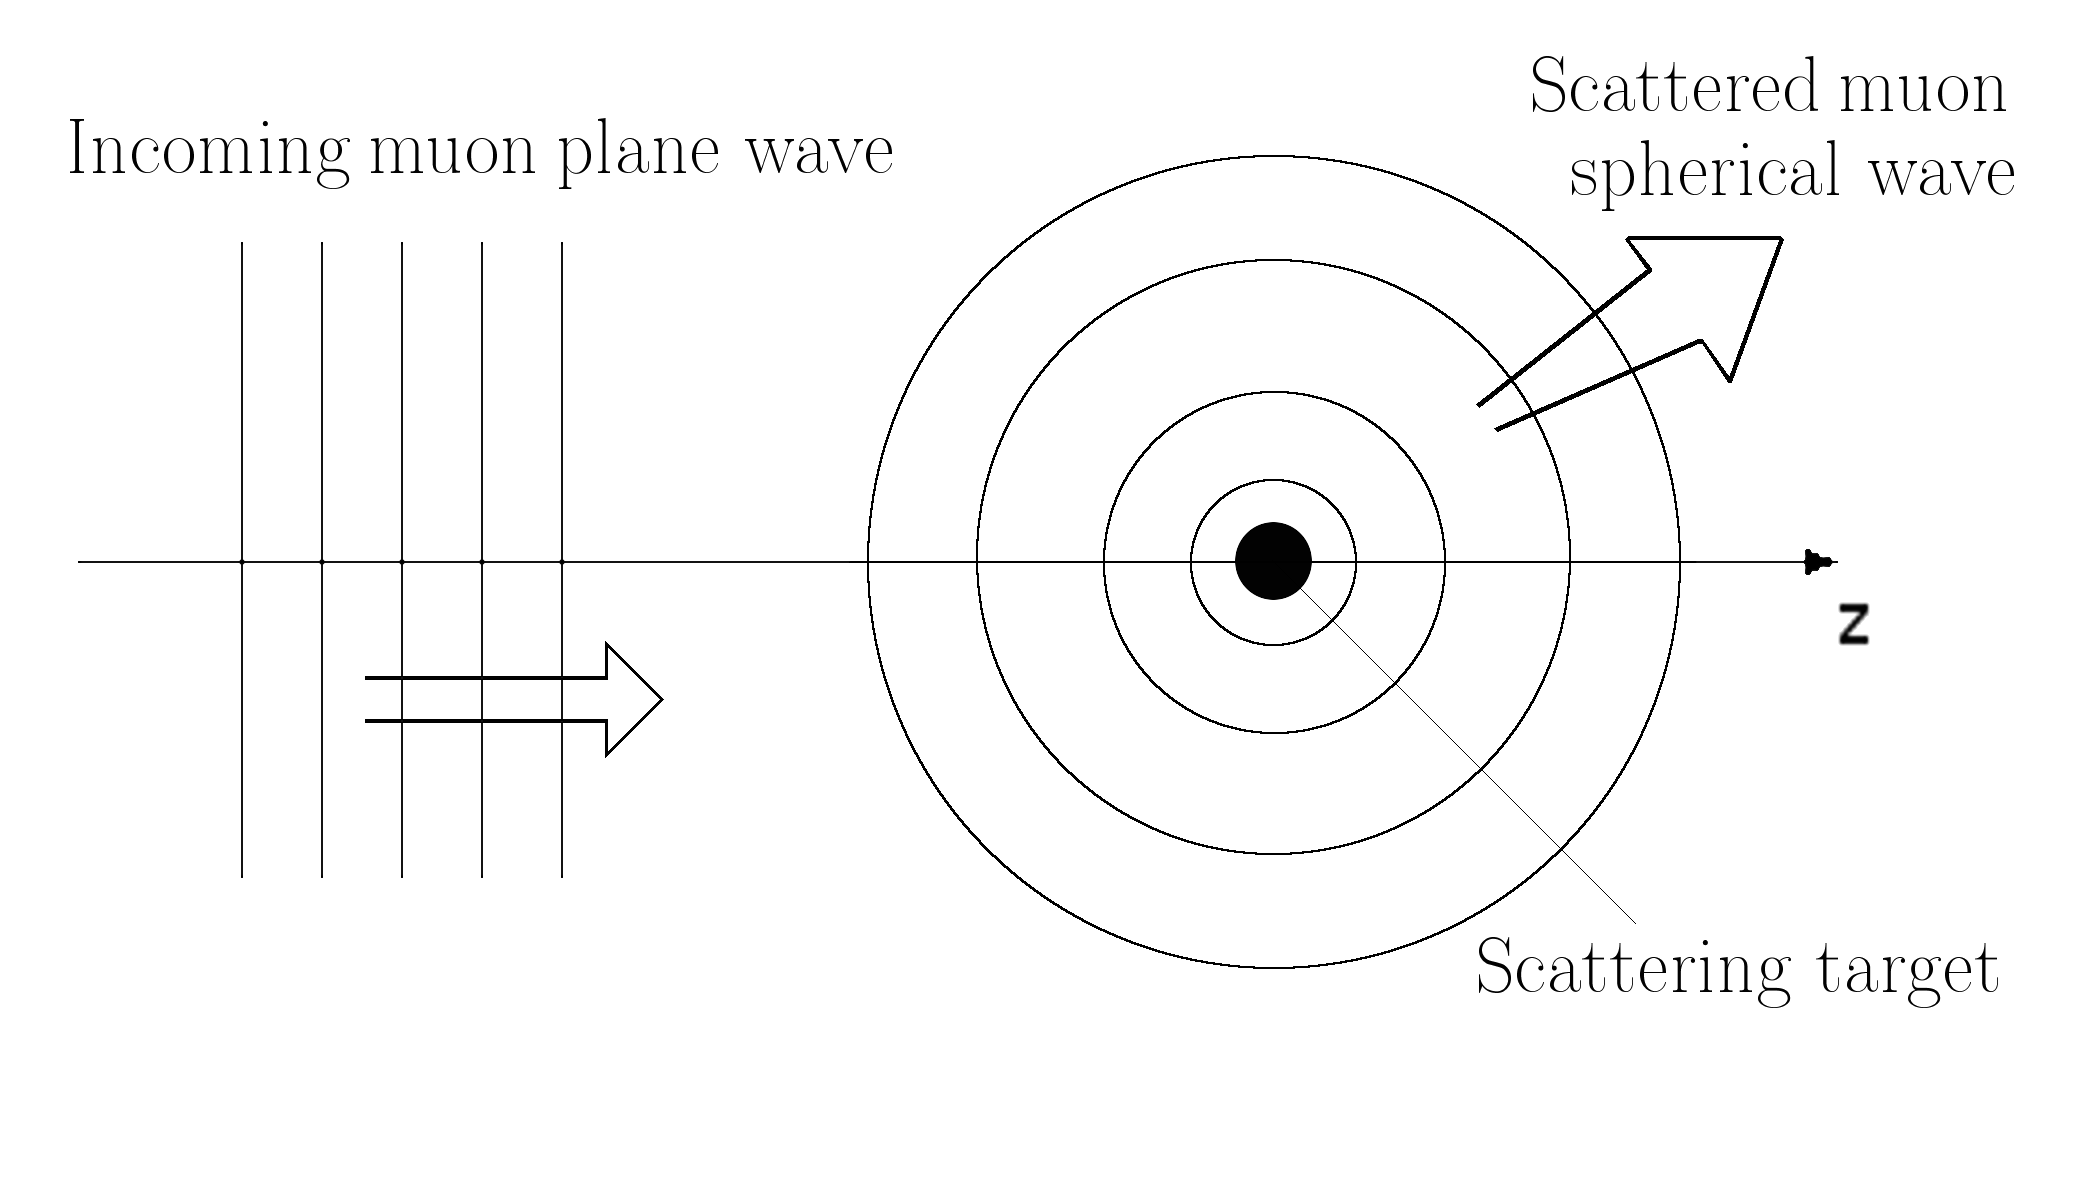
\includegraphics[width=\textwidth]{Figures/scattering_model_2} 
  \caption{Quantum scattering model.}
  \label{fig:qmscatteringmodel}
\end{figure}
Here there is an incoming plane wave (mathematically represented by $e^{ikz}$) and a spherical wave (represented by $e^{ikr}/r$). $r$ and $z$ are coordinates, $i$ is the imaginary unit, and $k$ is the wave number, classically related to the energy as $k=\sqrt{2mE}/\hbar$. Then basic quantum mechanics suggests that the solution to the Schr\"{o}dinger equation has the form
\begin{equation}
\label{eqn:scatteringwavefunction}
\psi (r,\theta)\approx A \left(e^{ikz}+f(\theta)\frac{e^{ikr}}{r}\right),
\end{equation}
where $A$ is the total amplitude and $f(\theta)$ is the scattering amplitude. The probability of the particle scattering in a particular direction is given by the amplitude squared, $|f(\theta)|^2$, and is the object of this derivation. Now, $\psi$ solves the differential (time-independent) Schr\"{o}dinger equation, which usually has the form
\begin{equation} \nonumber
-\frac{\hbar^2}{2m}\nabla^2\psi+V\psi=E\psi,
\end{equation}
where $V$ is the system potential and $E$ is the energy of the wavefunction. This can be expressed alternatively by assigning $Q\equiv V\psi\cdot{2m}/{\hbar^2}$ and recalling that $k=\sqrt{2mE}/\hbar$. Then
%
\begin{equation}
\label{eqn:schrodinger}
(\nabla^2+k^2)\psi=Q.
\end{equation}

The strategy is to solve Eqn. \ref{eqn:schrodinger} for $\psi$. A comparison of the solutions for $\psi$ from Eqns. \ref{eqn:scatteringwavefunction} and \ref{eqn:schrodinger} will yield the scattering amplitude $f(\theta)$. However, if Eqn. \ref{eqn:schrodinger} is solved for $\psi$ then it suggests that $\psi$ will be in integral form since  Eqn. \ref{eqn:schrodinger} is a differential equation. Therefore, some special techniques will be required. Note that it does not matter at this point that $Q$ is a function of $\psi$, since the task will be to compare the integrated solution of Eqn. \ref{eqn:schrodinger} with that of Eqn. \ref{eqn:scatteringwavefunction}. Moving forward, observe  that Eqn. \ref{eqn:schrodinger} may again be rewritten as
%
\begin{equation} \label{eqn:schrodinger_green_lhs}
(\nabla^2+k^2)\psi(\vec{r})=Q (\vec{r}) =\int \delta^3(\vec{r}-\vec{r}_0)Q(\vec{r}_0)d^3\vec{r}_0.
\end{equation}
Now it is natural to guess that there exists some function $G(\vec{r})$ such that
%
\begin{equation}
\label{eqn:psigreen}
\psi(\vec{r})=\int G(\vec{r}-\vec{r}_0)Q(\vec{r}_0)d^3\vec{r}_0,
\end{equation}
in which case
%
\begin{equation} \nonumber
(\nabla^2+k^2)\psi(\vec{r})=(\nabla^2+k^2)\int G(\vec{r}-\vec{r}_0)Q(\vec{r}_0) d^3\vec{r}_0,
\end{equation}
or
\begin{equation} \label{eqn:schrodinger_green_rhs}
(\nabla^2+k^2)\psi(\vec{r})=\int \big[(\nabla^2+k^2)G(\vec{r}-\vec{r}_0)\big]Q(\vec{r}_0) d^3\vec{r}_0.
\end{equation}
%
Combining Eqns. \ref{eqn:schrodinger_green_lhs} and \ref{eqn:schrodinger_green_rhs}, it can be seen that
\begin{align*}
\int \delta^3(\vec{r}-\vec{r}_0)Q(\vec{r}_0)d^3\vec{r}_0=\int \big[(\nabla^2+k^2)G(\vec{r}-\vec{r}_0)\big]Q(\vec{r}_0) d^3\vec{r}_0.
\end{align*}
Consequently, one comes to the conclusion that
%
\begin{equation}
\label{eqn:helmholtz}
(\nabla^2+k^2)G(\vec{r})=\delta^3(\vec{r}).
\end{equation}
If Eqn. \ref{eqn:helmholtz} seems familiar, it is because this is the Helmholtz equation with a delta function source. $G(\vec{r})$ is Green's function for the Helmholtz equation, and in this case it is the response to the delta function source. Now, if one accepts that there exists a well-known particular solution for Eqn. \ref{eqn:helmholtz}, then one could skip forward to the solution in Eqn. \ref{eqn:greensolution}; however, it will also be derived subsequently.

The usual strategy in solving systems like Eqn. \ref{eqn:helmholtz} is to Fourier transform both the Green's function and the delta function. Then creating the dummy variable $\vec{s}$, the transform yields
%
\begin{equation} \nonumber
G(\vec{r})=\frac{1}{(2\pi)^\frac{3}{2}}\int e^{i\vec{s}\cdot\vec{r}} g(\vec{s})d^3\vec{s},
\end{equation}
and
%
\begin{equation} \nonumber
\delta^3(\vec{r})=\frac{1}{(2\pi)^3}\int e^{i\vec{s}\cdot\vec{r}} d^3\vec{s}.
\end{equation}
Then from Eqn. \ref{eqn:helmholtz},
%
\begin{equation} \nonumber
\frac{1}{(2\pi)^\frac{3}{2}}\int (k^2e^{i\vec{s}\cdot\vec{r}}-s^2e^{i\vec{s}\cdot\vec{r}})g(\vec{s})d^3\vec{s}=\frac{1}{(2\pi)^3}\int e^{i\vec{s}\cdot\vec{r}}d^3\vec{s},
\end{equation}
it is clear that $g(\vec{s})=1/(2\pi)^{3/2}(k^2-s^2)$. Now all that is left is to find $G(\vec{r})$ from its transformation:
%
\begin{equation} \nonumber
G(\vec{r})=\frac{1}{(2\pi)^3}\int e^{i\vec{s}\cdot\vec{r}}\frac{d^3\vec{s}}{k^2-s^2}
\end{equation}
%
\begin{equation} \nonumber
G(\vec{r})=\frac{1}{(2\pi)^3}\int_0^\infty \frac{s}{k^2-s^2} \left(\int_0^\pi e^{isr\cos\theta}\sin\theta d\theta\right)ds \int_0^{2\pi}d\phi.
\end{equation}
The integration over $\phi$ is trivial, and the integration over $\theta$ can be done via $u$ substitution, with $u=\cos\theta$. The last integral is over $s$, and is
%
\begin{equation} \nonumber
G(\vec{r})=\frac{1}{2\pi^2r}\int_0^\infty\frac{s\sin{sr}}{k^2-s^2}ds=\frac{1}{4\pi^2r}\int_{-\infty}^\infty\frac{s\sin{sr}}{k^2-s^2}ds.
\end{equation}
This integral is not simple to solve, but it does have two poles at $s=k$ and $s=-k$, which implies the technique of choice should be to use Cauchy's integral formula for simple poles\footnote{This touches an area of mathematics known as the calculus of residues, and is based on the Laurent series.}:
%
\begin{equation}
\label{eqn:cauchy}
\oint \frac{f(z)}{z-z_0}dz=2\pi if(z_0),
\end{equation}
where the integral is done over some path in the complex plane and $z_0$ is the pole of interest which lies in the enclosed path (note: the integral is zero if there exist no poles in the enclosed path). It follows then that $f(z)$ is not simply any function, but a necessarily complex function which is closed. For this reason, the (strictly real) Green's function integral should be split up into two (strictly complex) functions, as depicted by Figure \ref{fig:complexgreen}. This can be done by expanding the $\sin sr$ term and factoring $k^2-s^2$:
%
\begin{equation}
\label{eqn:complexgreen}
G(\vec{r})=\frac{i}{8\pi^2r}\left[ \int_{-\infty}^\infty \frac{se^{isr}}{(s-k)(s+k)}ds-\int_{-\infty}^\infty \frac{se^{-isr}}{(s-k)(s+k)}ds \right].
\end{equation}
%
\begin{figure}
  \centering
    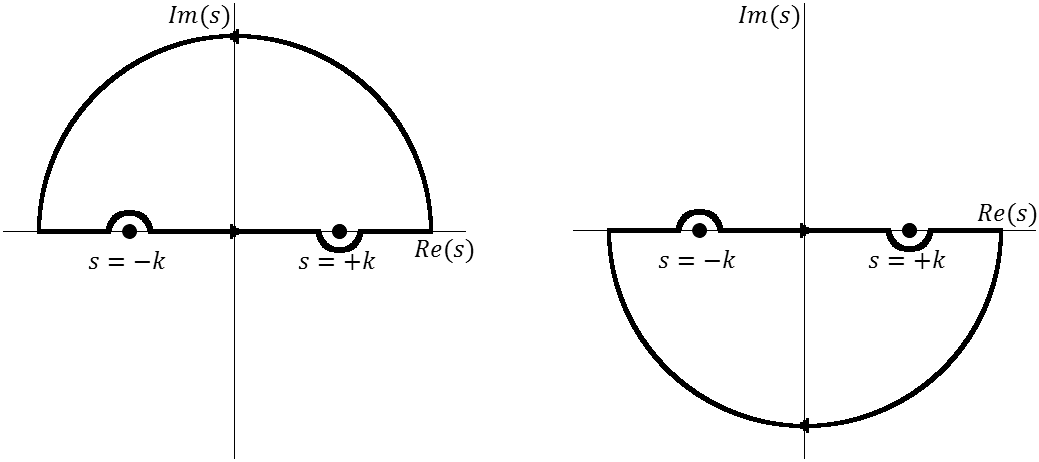
\includegraphics[width=\textwidth]{Figures/complexgreen} 
  \caption{Two parts of Green's function with their poles at $s=\pm k$, altered to be closed by a semicircle at $|s|=\pm\infty$.}
  \label{fig:complexgreen}
\end{figure}

Observe that in Eqn. \ref{eqn:complexgreen} the path integrals at $|s|=\pm\infty$ have been left out. This is because they do not contribute to the integral, since the first integrand corresponds to the left side of Figure \ref{fig:complexgreen} and goes like $e^{isr}$, hence going to zero at large positive imaginary numbers. Similarly, the second integrand goes like $e^{-isr}$ and goes to zero at large negative imaginary numbers.

Combining Eqns. \ref{eqn:cauchy} and \ref{eqn:complexgreen}, it can be seen that
%
\begin{equation}
\nonumber
G(\vec{r})=\frac{i}{8\pi^2r}[(i\pi e^{ikr})-(-i\pi e^{ikr})]=-\frac{e^{ikr}}{4\pi r}.
\end{equation}
This is a particular solution to the inhomogeneous Helmholtz equation. To get a general solution, the solution to the homogeneous Helmholtz equation must be added:
%
\begin{equation}
\label{eqn:greensolution}
G(\vec{r})=G_0(\vec{r})-\frac{e^{ikr}}{4\pi r};
\end{equation}
that is, $G_0(\vec{r})$ solves $(\nabla^2+k^2)G_0(\vec{r})=0$.

Using Eqn. \ref{eqn:psigreen} in conjunction with Eqn. \ref{eqn:greensolution} gives rise to the \emph{integrated} time-independent Schr\"{o}dinger equation:
%
\begin{equation} \label{eqn:integratedschrodinger}
\psi(\vec{r})=\psi_0 (\vec{r})-\frac{m}{2\pi\hbar^2}\int\frac{e^{ik|\vec{r}-\vec{r}_0|}}{|\vec{r}-\vec{r}_0|}V(\vec{r}_0)\psi(\vec{r}_0)d^3\vec{r}_0.
\end{equation}
%
That is, nothing has been said about the potential and so this equation is quite general. Eqn. \ref{eqn:integratedschrodinger} gives the recursive form for $\psi$. Let $g=-me^{ik|\vec{r}-\vec{r}_0|}/2\pi\hbar^2|\vec{r}-\vec{r}_0|$. Then Eqn. \ref{eqn:integratedschrodinger} says that
%
\begin{equation} \nonumber
\psi=\psi_0+\int gV\psi = \psi_0+\int gV (\psi_0+\int gV\psi).
\end{equation}
%
Applying this recursion several times gives the Born series:
%
\begin{equation}\nonumber
\psi=\psi_0+\int gV\psi_0+\int \int gVgV\psi_0 + \int \int \int gVgVgV\psi_0 + ...
\end{equation}
%
The zeroth term is exact if there is no scattering whatsoever (i.e. $V=0$) and the first term is accurate if the scattering potential is ``weak'' (that is, if $V$ is small enough for the second term to be neglected). For the purposes of this derivation, first order will be a sufficient approximation for $\psi$. Then
%
\begin{equation} \nonumber
\psi=\psi_0+\frac{m}{2\pi\hbar^2}\int\frac{e^{ik|\vec{r}-\vec{r}_0}}{|\vec{r}-\vec{r}_0|}V(\vec{r}_0)\psi_0(\vec{r}_0) d^3\vec{r}_0.
\end{equation}

Recall that the strategy was to compare this solution of the Helmholtz equation with the wavefunction from the quantum scattering model (Eqn. \ref{eqn:scatteringwavefunction}) in order to find the scattering amplitude, $f(\theta)$. Doing so yields
%
\begin{equation} \nonumber
f(\theta)=-\frac{r}{e^{ikr}}\frac{m}{2\pi\hbar^2A}\int\frac{e^{ik|\vec{r}-\vec{r}_0|}}{|\vec{r}-\vec{r}_0|}V(\vec{r}_0)\psi_0(\vec{r}_0)d^3\vec{r}_0.
\end{equation}
%

The Coulomb potential goes as $1/r^2$, and as such $V(\vec{r}_0)$ is localized about $\vec{r}_0=0$. Since particles are observed far away from their scattering centers, it is advantageous to make use of the fact that $\vec{r} \gg \vec{r}_0$. However, caution must be taken, since one must evaluate the exponential and non-exponential terms separately, for they are of separate orders. For the non-exponential terms, this is simple, since
%
\begin{equation}\nonumber
\frac{r}{|\vec{r}-\vec{r}_0|}\approx1.
\end{equation}
%
The exponential terms look like
%
\begin{equation}\nonumber
e^{ik(|\vec{r}-\vec{r}_0|-r)},
\end{equation}
and so it is useful to expand the absolute value as
\begin{equation}\nonumber
|\vec{r}-\vec{r}_0|^2=r^2+r_0^2-2\vec{r}\cdot\vec{r}_0\approx r^2\left(1-2\frac{\vec{r}\cdot\vec{r}_0}{r^2}\right),
\end{equation}
%
or simply
%
\begin{equation} \nonumber |\vec{r}-\vec{r}_0|\approx r-\hat{r}\cdot\vec{r}_0. \end{equation}
%
This leaves
%
\begin{equation} \label{eqn:generalscattering}
f(\theta)=\frac{m}{2\pi\hbar^2}\int
e^{-ik\hat{r}\cdot\vec{r}_0}
V(\vec{r}_0)
e^{ik\hat{z}\cdot\vec{r}_0}
d^3\vec{r}_0,
\end{equation}
%
Now define $\vec{\kappa}\equiv k(\hat{z}-\hat{r})$ such that $\kappa=2k\sin{\theta/2}$. The exponential term becomes
%
\begin{equation} \nonumber
e^{i\vec{\kappa}\cdot\vec{r}_0}=e^{i\kappa r_0\cos{\theta_0}}.
\end{equation}
Furthermore, the form of the potential $V$ is known. Since the scattering for the low-$Z$ target happens at low temperatures, it is possible to use the Fermi-Thomas approximation for screening \cite{ashcroft}. This modifies the Maxwell equation 
\begin{align*}
\nabla^2 V(r) = -\frac{\rho}{\epsilon_0}
\end{align*}
to
\begin{equation} \nonumber
(\nabla^2-b^2)V(r)=-\frac{Q}{\epsilon_0}\delta(r),
\end{equation}
%
where $\rho$ is the charge density, $b$ is some screening constant, $\epsilon_0$ is the permittivity of free space, and $Q$ is the charge of the potential (in this case, the atomic number $Z$). The solution is
\begin{equation} \nonumber
V(r)=\frac{Q}{4\pi\epsilon_0}\frac{e^{-br}}{r}.
\end{equation}
Then the quantum scattering equation (Eqn. \ref{eqn:generalscattering}) becomes
%
\begin{equation} \nonumber
f(\theta)\propto \int e^{i\kappa r_0\cos(\theta_0)}e^{-br_0}r_0\sin(\theta_0)dr_0 d\theta_0 d\phi_0,
\end{equation}
where the amplitude terms have been left out since $|f(\theta)|^2$ is normalized anyway. Here it is seen that there does exist some $\theta$ dependence in $f(\theta)$ (by virtue of $\kappa$). The integral over $\phi_0$ is trivial, and the integral over $\theta_0$ can be done via $u$ substitution, with $u=\cos\theta_0$. This leaves
\begin{equation} \nonumber
f(\theta)\propto \frac{1}{\kappa}\int_0^\infty e^{-br_0}\sin(\kappa r_0) dr_0,
\end{equation}
%
which has the solution
\begin{equation}\nonumber
f(\theta)\propto\frac{1}{b^2+\kappa^2}.
\end{equation}
For classical Rutherford scattering, $b\rightarrow 0$. Recalling that $\kappa=2k\sin{\theta/2}$ yields the final Rutherford scattering distribution:
\begin{align}
|f(\theta)|^2 &\propto \frac{1}{\sin^4 \frac{\theta}{2}}=\frac{1}{\left(\sin^2 \frac{\theta}{2}\right)^2}=\frac{1}{\left(\frac{1}{2}\left[1-\cos^2\left(2\cdot\frac{\theta}{2}\right)\right]\right)^2},\nonumber \\
|f(\theta)|^2  &\propto\frac{1}{(1-\cos^2{\theta})^2}. \label{eqn:rutherford}
\end{align}

Only the tail of Eqn. \ref{eqn:rutherford} should be used since it blows up at $\theta=0$. This may seem like a contradiction, since the Born series was truncated at the weak potential term (the first nontrivial term), and hence the incoming muons should not scatter much at all! In fact, the muons are not scattering much at all for each individual atom they encounter. Over the entire absorber, however, some muons will have a net scattering angle which is small (and therefore should not be approximated by the Rutherford tail) whereas others will have a large net scattering angle (and are well represented by Eqn. \ref{eqn:rutherford}). Many weak potentials can still induce a relatively large scattering angle.
\\
\Section{Energy Straggling in G4Beamline} \label{sec:g4blstraggling}

G4Beamline uses the in-house straggling model described by GEANT4 in \cite{geant4}.  GEANT4 has determined that a ``thick absorber'' occurs when the following conditions are met:
\begin{align}\label{eqn:G4StragglingThickTest}
\begin{split}
|\delta E| &> \kappa T_c  \\
T_{max} &\le 2T_c,
\end{split}
\end{align}
where $\delta E$ is the energy loss, $\kappa$ is the Vavilov limit parameter, is the $T_c$ is the kinetic energy cut of $\delta$-electrons, and $T_{max}$ is the maximum transferrable kinetic energy between the incoming particle and target electron. These symbols can also be found in the Definition of Terms at the beginning of this document.

For thick absorbers, the energy loss is sampled according to a simple Gaussian distribution with average equal to the Bethe-Bloch energy loss (Eqn. \ref{eqn:bethebloch}) and a standard deviation according to Bohr's variance (Eqn. \ref{eqn:bohrvariance}).

If these conditions are not met, a ``thin absorber" algorithm is called. Here, atoms are assumed to have only two energy levels with binding energies $E_1$ and $E_2$. The interacting muon can then lose energy via excitation, yielding an energy loss of $E_1$ or $E_2$, or lose energy via $\delta$ ray production, yielding an energy loss according to $ g(E) \propto 1/E^2 $, or (more likely) some combination or weighted average of the two. $g(E)$ may then be normalized:
\begin{equation}
\int_{E_0}^{T_{up}} g(E) dE = 1 \rightarrow g(E)=\frac{E_0 T_{up}}{T_{up}-E_0}\frac{1}{E^2},
\label{eqn:G4StragglingIonization}
\end{equation}
where $E_0$ is the ionization energy of the atom in question and $T_{up}$ is some kinetic energy cutoff (either the production threshold for delta rays or the maximum transferrable energy, whichever is smaller).

The probability for obtaining any one of these energy losses is given by the macroscopic cross section, $\Sigma_i$, where $i=1,2,3$. For excitation ($i=1,2$), the cross section has a form similar to the deterministic Bethe-Bloch equation (Eqn. \ref{eqn:bethebloch}):
\begin{equation}\label{eqn:G4StragglingCrossSectionExcitation}
\Sigma_i=C\frac{f_i}{E_i}\frac{\ln(2m_e c^2(\beta\gamma)^2/E_i)}{\ln(2m_e c^2(\beta\gamma)^2/I)}(1-r).
\end{equation}
Here, $C$ and $r=0.55$ are model parameters with $r$ describing the relative contribution of excitation to ionization, $f_i$ are the relative oscillator strengths of the energy levels of $E_i$, $I$ is the average ionization energy, and the other symbols have their usual meaning. For continuous energy loss, the cross section is given by
\begin{equation}\label{eqn:G4StragglingCrossSectionIonization}
\Sigma_3=C\frac{T_{up}-E_0}{T_{up}E_0\ln(T_{up}/E_0)}r.
\end{equation}

The oscillator strengths are relative to one another and hence should satisfy
\begin{equation}\label{eqn:G4StragglingOscillatorConstraint1}
f_1+f_2=1.
\end{equation}
The next constraint comes from \cite{bichsel1988} and states that all the energy levels should be weighted and add logarithmically to the total ionization energy:
\begin{equation}\label{eqn:G4StragglingOscillatorConstraint2}
f_1 \ln E_1 + f_2 \ln E_2 = \ln I.
\end{equation}
Moreover, $f_1$ and $f_2$ can be thought of as representing the relative number of loosely and tightly bound electrons. Then using the first constraint, it is easy to see that the absolute number of loosely bound electrons are $Z\cdot f_1$ and the absolute number of tightly bound electrons are $Z\cdot f_2$ (since $Z\cdot f_1+Z\cdot f_2=Z$). For modeling purposes, GEANT4 has placed emperical initial conditions on these parameters:
\begin{align} \label{eqn:G4StragglingOscillatorConstraint3}
f_2 & = 0 & \text{   for   } Z=1,\\
f_2 & = 2/Z & \text{     for     } Z\ge 2,\\
E_2 & = 10 \text{ eV } Z^2,\\
E_0 &= 10 \text{ eV}.
\end{align}
From these, $f_1$ and $E_1$ can be found from Eqns. \ref{eqn:G4StragglingOscillatorConstraint1} and \ref{eqn:G4StragglingOscillatorConstraint2} given a particular muon through a particular material (from which $Z$, $I$, $\beta$, and the like are taken).

Finally, an energy loss for a thin absorber can be sampled. For the contribution due to excitation, two numbers $n_1$ and $n_2$ are sampled randomly from a Poisson distribution. These numbers represent the relative contributions of the energy levels of $E_1$ and $E_2$, respectively:
\begin{equation}\nonumber
\epsilon_{exc}=n_1 E_1 + n_2 E_2.
\end{equation}

The contribution due to ionization can be found by inverting the cumulative distribution function of $g(E)$ (see Eqn. \ref{eqn:G4StragglingIonization}):
\begin{equation}\nonumber
G(E)=\int_{E_0}^E g(E) dE \rightarrow E=\frac{E_0}{1-u\frac{T_{up}-E_0}{T_{up}}},
\end{equation}
where $u$ is uniformly randomly selected from $[0,1]$. However, this treatment so far has only been exectued for a single ionization. For an absorber of length $L$, the number of ionizations $n_3$ is again sampled from a Poisson distribution. Then the total energy loss for thin absorbers is
\begin{equation}\label{G4StragglingThin}
\epsilon = n_1 E_1 + n_2 E_2 + \sum_{j=1}^{n_3} \frac{E_0}{1-u_j \frac{T_{up}-E_0}{T_{up}}}.
\end{equation}

It should be noted that \cite{geant4} does make a brief mention of a width correction algorithm. This algorithm allegedly decreases the dependence of the results on kinetic energy cuts and step sizes and works for any thickness of material. However, the section in the manual is less than a page long and purely conceptual without any mathematics or data on which to elaborate. The width correction algorithm is relevant to this work in order to make a fair comparison and understand why this work and G4Beamline disagree in some places.

Finally, the GEANT4 straggling routine can be summarized as such:
\begin{enumerate}
\item{Determine if absorber is ``thick'' via Eqn. \ref{eqn:G4StragglingThickTest}.}
\item{If absorber is thick, use Gaussian distribution with mean $\mu = \left<dE/dx\right>$ (from Eqn. \ref{eqn:bethebloch}) and standard deviation from Eqn. \ref{eqn:bohrvariance}.}
\item{If absorber is ``thin'', use Eqn. \ref{G4StragglingThin}.
	\begin{itemize}
	\item{Select $n_1$, $n_2$, and $n_3$ from a Poisson distribution.}
	\item{Select $u_j$ from a uniform distribution on $[0,1]$ (where $j=1...n_3$).}
	\item{Find $E_2$, $f_2$, and $E_0$ from Eqn. \ref{eqn:G4StragglingOscillatorConstraint3}.} 
	\item{Find $E_1$ from Eqns. \ref{eqn:G4StragglingOscillatorConstraint1} and \ref{eqn:G4StragglingOscillatorConstraint2}.}
	\end{itemize}
	}
\item{Apply width correction algorithm.}
\end{enumerate}
%---------------------------------------------------------------------------------------------------------------------------------------------------------------------
\Section{Multiple Scattering in G4Beamline} \label{sec:g4blscattering}\par
The G4Beamline scattering model in \cite{g4bl} uses the GEANT4 Urb\'{a}n model \cite{geant4}, and again parameterizes according to experimental data and Lewis theory \cite{lewis}. For this section, the scattering distribution is $g(u)$, where $u=\cos\theta$ and $\theta$ is the scattering angle.

Based on the models available, it can be inferred that the function responsible for the sampling of the angular distribution, $g(u)$, is based off both the Goudsmit-Saunderson treatment of scattering \cite{gs} and Rutherford scattering. One fundamental result from Goudsmit and Saunderson is that for small angles, the scattering distribution is Gaussian. Recall that Rutherford scattering was derived in Section \ref{sec:ICOOLScattering} and resulted in Eqn. \ref{eqn:rutherford}. It should be noted that the shape of $g(u)$ was chosen empirically, and is
%
\begin{equation}\label{eqn:g4blgu}
g(u)=q_g\left[p_g g_1(u)+(1-p_g)g_2(u)\right]+(1-q_g)g_3(u),
\end{equation}
%
where $0\leq p_g,q_g\leq 1$ and
%
\begin{align*}\nonumber
g_1(u)&=C_1e^{-a(1-u)} & -1\le u_0\le u\le 1\\
g_2(u)&=C_2\frac{1}{(b_r-u)^{d_r}} & -1\le u\le u_0\le 1\\
g_3(u)&=C_3 & -1\le u \le 1
\end{align*}
%
are normalized over $[-1,1]$, where $C_i$ are normalization constants and $a$, $b_r$, $d_r$, and $u_0$ are empirical parameters. All of these parameters will be discussed in this section, and can be found in Table \ref{tbl:g4blgu_parameters}. 

\newcolumntype{A}{ >{\centering\arraybackslash} m{2.5cm} } % centered horizontally and vertically
\newcolumntype{B}{ >{\centering\arraybackslash} m{4.75cm} }
\newcolumntype{C}{ >{\centering\arraybackslash} m{1.5cm} }
\begin{table}
\caption*{\textbf{G4Beamline Scattering Distribution Parameters}}
\begin{tabularx}{\textwidth}{| A | B | B | C |}
\hline \hline
	\textbf{Parameter} & \textbf{Physical Meaning} & \textbf{Found Via} & \textbf{Eqn.} \\ \hline
	$C_1$, $C_2$, and $C_3$ & Normalization constants & Normalization & $N/A$ \\ \hline
	$a$ & Related to Gaussian-like $\sigma$ & Relating the Gaussian-like behavior of $g_1(u)$ to Highland-like theory \cite{highland} & \ref{eqn:geanta} \\ \hline
	$u_0$ & The boundary between the Gaussian-like $g_1(u)$ and the Rutherford-like $g_2(u)$ & Emperical parameterization & \ref{eqn:geantu0} \\ \hline
	$d_r$ & The Rutherford-like exponent in $g_2(u)$ & Emperical parameterization & \ref{eqn:geantd} \\ \hline
	$p_g$ & Relative contribution of the Gaussian-like $g_1(u)$ to the Rutherford-like $g_2(u)$ & Demanding continuity & \ref{eqn:geantp} \\ \hline
	$b_r$ & Relative $u$ offset of the Rutherford-like $g_2(u)$ & Demanding smoothness & \ref{eqn:geantb} \\ \hline
	$q_g$ & The relative contribution of the varying functions $g_1(u)$ and $g_2(u)$ to the constant function $g_3(u)$ & Demanding that $g$ gives the same mean value as Lewis theory & \ref{eqn:geantq}\\
\hline
\end{tabularx}
\caption[G4Beamline scattering distribution parameters.]{The nine parameters of the scattering distribution used by G4Beamline (see Eqn. \ref{eqn:g4blgu}).}
\label{tbl:g4blgu_parameters}
\end{table}


Observe that for small angles, $g(u)$ is nearly Gaussian since $\exp{(1-u)}=\exp{(1-\cos\theta)}\approx\exp{(\theta^2/2)}$. For large angles, $g(u)$ resembles the Rutherford dependence of Eqn. \ref{eqn:rutherford} for $b_r\approx 1$ and $d_r$ close to 2. Moreover, at small $q_g$ the shape of $g(u)$ is nearly constant since the constant function $g_3(u)$ dominates.

While Eqn. \ref{eqn:g4blgu} is the main point of this section, it would be incomplete without detailing the nine parameters mentioned. The $C_i$ (with $i=1,2,3$) are normalization constants. $a$, $u_0$, and $d_r$ are chosen based off theoretical and experimental data and are a bit more interesting. Finally, $p_g$, $q_g$, and $b_r$ can be found using constraints. 

\noindent \textit{\large{Finding $a$}}

Observe from Eqn. \ref{eqn:g4blgu} that $a$ only appears in $g_1(u)$. Further observe from Eqn. \ref{eqn:g4blgu} that $g_1(u)$ is only valid for $u$ close to 1. Since $u=\cos\theta$ (where $\theta$ is the scattering angle), $g_1(u)$ must be the part of $g(u)$ that determines small angle scattering. 

It has already been noted that $g_1(u)$ is approximately Gaussian for $u$ close to 1. Highland \cite{highland} provided an estimate for the width of the (approximate) Gaussian scattering distribution. Let the width of this Gaussian distribution be $\theta_0$. Lynch and Dahl \cite{lynchdahl} gave corrections to Highland's form of $\theta_0$ in 1991. If $\theta_0$ truly is the width of the Gaussian scattering distribution, then it follows that
%
\begin{equation}\nonumber
g_1(u) \underset{\sim}{\propto} \exp{\Big(-\frac{\theta^2}{2\theta_0^2}\Big)} \approx \exp\Big(\frac{1}{2}\cdot\frac{1-\cos\theta}{1-\cos\theta_0}\Big),
\end{equation}
%
where $\underset{\sim}{\propto}$ means ``approximately proportional to''. Recall from Eqn. \ref{eqn:g4blgu} that
\begin{equation}\nonumber
g_1(u)\propto \exp{(-a(1-u))}.
\end{equation}
Then it is reasonable to choose $a$ as
%
\begin{equation}
a=\frac{0.5}{1-\cos\theta_0}
\label{eqn:geanta}
\end{equation}
%
so that
%
\begin{equation}\nonumber
\exp{(-a(1-u))}=\exp\Big(\frac{1}{2}\cdot\frac{1-\cos\theta}{1-\cos\theta_0}\Big).
\end{equation}
%

 For heavy charged particles (such as muons), the model for $\theta_0$ has been modified even more from Lynch and Dahl by GEANT4 \cite{geant4}. Its form is now chosen by GEANT4 \cite{geant4} as
%
\begin{equation}\label{g4bltheta0}
\theta_0=\frac{13.6 \text{MeV}}{\beta c p}z_{ch}\sqrt{\frac{t}{X_0}\Big[ 1+0.105\ln\Big(\frac{t}{X_0}\Big)+0.0035\Big(\ln\Big(\frac{t}{X_0}\Big)\Big)^2 \Big]}\Big(1-\frac{0.24}{Z(Z+1)}\Big).
\end{equation}

\noindent \textit{\large{Finding $u_0$}}

Observe from Eqn. \ref{eqn:g4blgu} that the parameter $u_0$ is the boundary between the Gaussian-like $g_1(u)$ and the Rutherford-like $g_2(u)$. GEANT4 \cite{geant4} has chosen $u_0$ as
\begin{equation}
u_0=1-\frac{3}{a}.
\label{eqn:geantu0}
\end{equation}
It is assumed that this parameter has been chosen as such based on emperical results, but no formal explaination is given. While GEANT4 \cite{geant4} does not elaborate on this parameterization, validation in Section \ref{sec:validation} will show that this choice is reasonable.

\noindent \textit{\large{Finding $d_r$}}


Observe from Eqn. \ref{eqn:g4blgu} that the parameter $d_r$ the Rutherford-like exponent. Note that a classical Rutherford distribution would have $d_r=2$. For heavy particles like muons, the parameter $d_r$ has been chosen by GEANT4 \cite{geant4} as
\begin{equation}
d_r=2.40-0.027Z^{\frac{2}{3}}.
\label{eqn:geantd}
\end{equation}
It is assumed that this parameter has been chosen as such based on emperical results, but no formal explaination is given. While GEANT4 \cite{geant4} does not elaborate on this parameterization, validation in Section \ref{sec:validation} will show that this choice is reasonable.

\noindent \textit{\large{Finding $p_g$}}

Now $p_g$ will be found using constraints on the scattering distribution $g(u)$. Observe from Eqn. \ref{eqn:g4blgu} that the parameter $p_g$ is the relative contribution of the Gaussian-like $g_1(u)$ to the Rutherford-like $g_2(u)$. It is reasonable to demand that $g(u)$ be continuous and smooth on $[-1,1]$. Taking continuity and smoothness at $u=u_0$ yields the following constraints:
%
\begin{align}
p_g g_1(u_0)&=(1-p_g)g_2(u_0), \label{eqn:constraint_smoothness}\\
a\cdot p_g g_1(u_0)&=(1-p_g)g_2(u_0)\cdot\frac{d_r}{b_r-u_0}. \label{eqn:constraint_continuity}
\end{align}
%
From Eqn. \ref{eqn:constraint_smoothness}, it is easy to see that
%
\begin{equation}
p_g=\frac{g_2(u_0)}{g_1(u_0)+g_2(u_0)}.
\label{eqn:geantp}
\end{equation}
%

\noindent \textit{\large{Finding $b_r$}}

Observe from Eqn. \ref{eqn:g4blgu} that the parameter $b_r$ is the relative $u$ offset of the Rutherford-like distribution. For a classical Rutherford distribution, $b_r=1$. From Eqn. \ref{eqn:constraint_continuity},
%
\begin{equation}\nonumber
a=\frac{d_r}{b_r-u_0}.
\end{equation}
%
Rearranging this yields
%
\begin{equation}
b_r=\frac{a}{d_r}+u_0.
\label{eqn:geantb}
\end{equation}
%
\noindent \textit{\large{Finding $q_g$}}

Lastly, $q_g$ is found by knowing that $g(u)$ must give the same mean value as Lewis theory. Observe from Eqn. \ref{eqn:g4blgu} that the parameter $q_g$ is the relative contribution of the varying functions $g_1(u)$ and $g_2(u)$ to the constant function $g_3(u)$. GEANT4 \cite{geant4} shows that
%
\begin{equation}
q_g=\frac{(1-\frac{\lambda_{10}-\lambda_{11}}{\lambda_{10}})^{\frac{t}{\lambda_{10}-\lambda_{11}}}}{p_g\left<u\right>_1+(1-p_g)\left<u\right>_2},
\label{eqn:geantq}
\end{equation}
where $\lambda_{10}$ is the value of the first transport free mean path at the beginning of the step, $\lambda_{11}$ is this value at the end of the step, $t$ is the true path length, and $\left<u\right>_i$ is the mean value of $u$ computed from the distribution $g_i(u)$.

%\noindent \textit{\large{Summary}}

%In summary, the scattering model used by G4Beamline is based on the Geant4 model, which includes Lewis theory. The full form of the scattering equation is given by Eqn. \ref{eqn:g4blgu}. %This model has 9 parameters: 

\Chapter{Stochastic Processes in COSY Infinity}\label{chp:cosy}
In this chapter, the new algorithms implemented into COSY Infinity in the framework of this work are elaborated upon. First, energy straggling via Landau theory is detailed, including novel corrections. Next, the multiple scattering algorithm (which resembles the G4beamline algorithm discussed in Section~\ref{sec:g4blscattering}) and its implementation are discussed. Finally, the transverse displacement and temporal displacement algorithms are shown.

\Section{Energy Straggling in COSY} \label{sec:COSYStraggling}\par
For energy loss, COSY uses the Bethe-Bloch equation (Eq. \eqref{eqn:bethebloch}) to find the mean energy loss. This can be done in the transfer map paradigm since average energy loss is a deterministic effect. However, this work is concerned with simulating realistic stochastic fluctuations about the average energy loss. For this reason, this work has implemented Landau theory \cite{landau} to describe the straggling distribution. Landau theory is discussed in detail in Section~\ref{ssc:ICOOLStragglingLandau}. 

\iffalse
Other straggling models which were investigated were
\begin{itemize}
\item{Functionalization}
\item{Urb\'{a}n model \cite{geant4}}
\item{Vavilov theory \cite{vavilov}}
\item{Edgeworth series \cite{edgeworth}}
\item{Convolution method (compound Poisson method) \cite{kellerer}}
\item{Landau/Gaussian convolution \cite{hancock}}
\item{Blunck-Liesegang theory \cite{blunck}}
\end{itemize}
However, Landau theory proved to be the best fit. It was chosen over the Vavilov distribution in particular due to a complication where the Vavilov tail was abruptly cut off under certain circumstances.
\fi

Due to its long tail, the average of the Landau distribution is undefined. This is clearly nonphysical. Recall from Eq. \eqref{eqn:landauParameter} that the universal Landau parameter is
\begin{align*}
\lambda=\frac{\epsilon-\left<\epsilon\right>}{\xi}-(1-C_{Euler})-\beta ^2 -\ln (\xi/T_{max}),
\end{align*}
where $\epsilon$ is the energy loss, $C_{Euler}$ is the Euler constant ($\approx 0.577$), $\beta=v/c$ is the velocity in units of $c$, and $T_{max}$ is the maximum transferable energy from an incident muon to an electron at rest. However, this means that fluctuations about the mean energy loss $\left(\epsilon-\left<\epsilon\right>\right)$ are also divergent given enough samples. This can be seen as follows:
\begin{align*}
\left<\lambda\right>&\rightarrow\infty\\
\left<\frac{\epsilon-\left<\epsilon\right>}{\xi}-(1-C_{Euler})-\beta ^2 -\ln (\xi/T_{max})\right>&\rightarrow\infty\\
\left<\frac{\epsilon-\left<\epsilon\right>}{\xi}\right>&\rightarrow\infty\\
\left<\left(\epsilon-\left<\epsilon\right>\right)\right>&\rightarrow\infty.
\end{align*}
The possibility of divergence results in a sensitivity to step size since smaller steps effectively produce a large sample size. In order to combat this, an artificial cutoff is given to $\lambda$ such that the average Landau $\epsilon$ is equal to the average Bethe-Bloch energy loss $\left<\epsilon\right>$. That is, it is required that
\begin{align*}
\left<\lambda\right>&=\left<\frac{\epsilon-\left<\epsilon\right>}{\xi}\right>-(1-C_{Euler})-\beta^2-\ln(\xi/T_{max})\\
&=-(1-C_{Euler})-\beta^2-\ln(\xi/T_{max}).
\end{align*}
If the cutoff is $\lambda_{max}$, then $\left<\lambda\right>$ can be calculated by the definition of an average over the range $[0,\lambda_{max}]$:
\begin{align*}
\left<\lambda\right>=\frac{\int_0 ^{\lambda_{max}} \lambda * f(\lambda) d\lambda}{\int_0 ^{\lambda_{max}}f(\lambda) d\lambda}.
\end{align*}
The task then is to numerically find $\lambda_{max}$ such that it satisfies
\begin{align*}
\frac{\int_0 ^{\lambda_{max}} \lambda * f(\lambda) d\lambda}{\int_0 ^{\lambda_{max}}f(\lambda) d\lambda}=-(1-C_{Euler})-\beta^2-\ln(\xi/T_{max}).
\end{align*}
GEANT version 3.21 \cite{geant3.21} suggests the following form for $\lambda_{max}$:
\begin{equation} \label{eqn:landauCutoffsGeant3}
\lambda_{max}=0.60715+1.1934\left<\lambda\right>+(0.67794+0.052382\left<\lambda\right>)\exp[0.94753+0.74442\left<\lambda\right>)]
\end{equation}
(note that GEANT4 does not have a section on the Landau cutoff since the Urb\'{a}n straggling model\footnote{Note that the Urb\'{a}n straggling model should not be confused with the Urb\'{a}n multiple scattering model.} is used instead). However, a plot of required cutoffs ($\lambda_{max}$) vs. desired means ($\left<\lambda\right>$) was produced independently in this work with muon ionization cooling parameters in mind. The form suggested by GEANT3 (see, e.g., Eq. \eqref{eqn:landauCutoffsGeant3}) was used to fit the plot in Figure~\ref{fig:landau_cutoffs}. The determined form of the function is
\begin{equation}\label{eqn:landauCutoffs}
\lambda_{max}=0.517891+1.17765\left<\lambda\right>+(0.476074+0.00880733\left<\lambda\right>)\exp[1.15467+0.984008\left<\lambda\right>].
\end{equation}

\begin{figure}
  \centering
    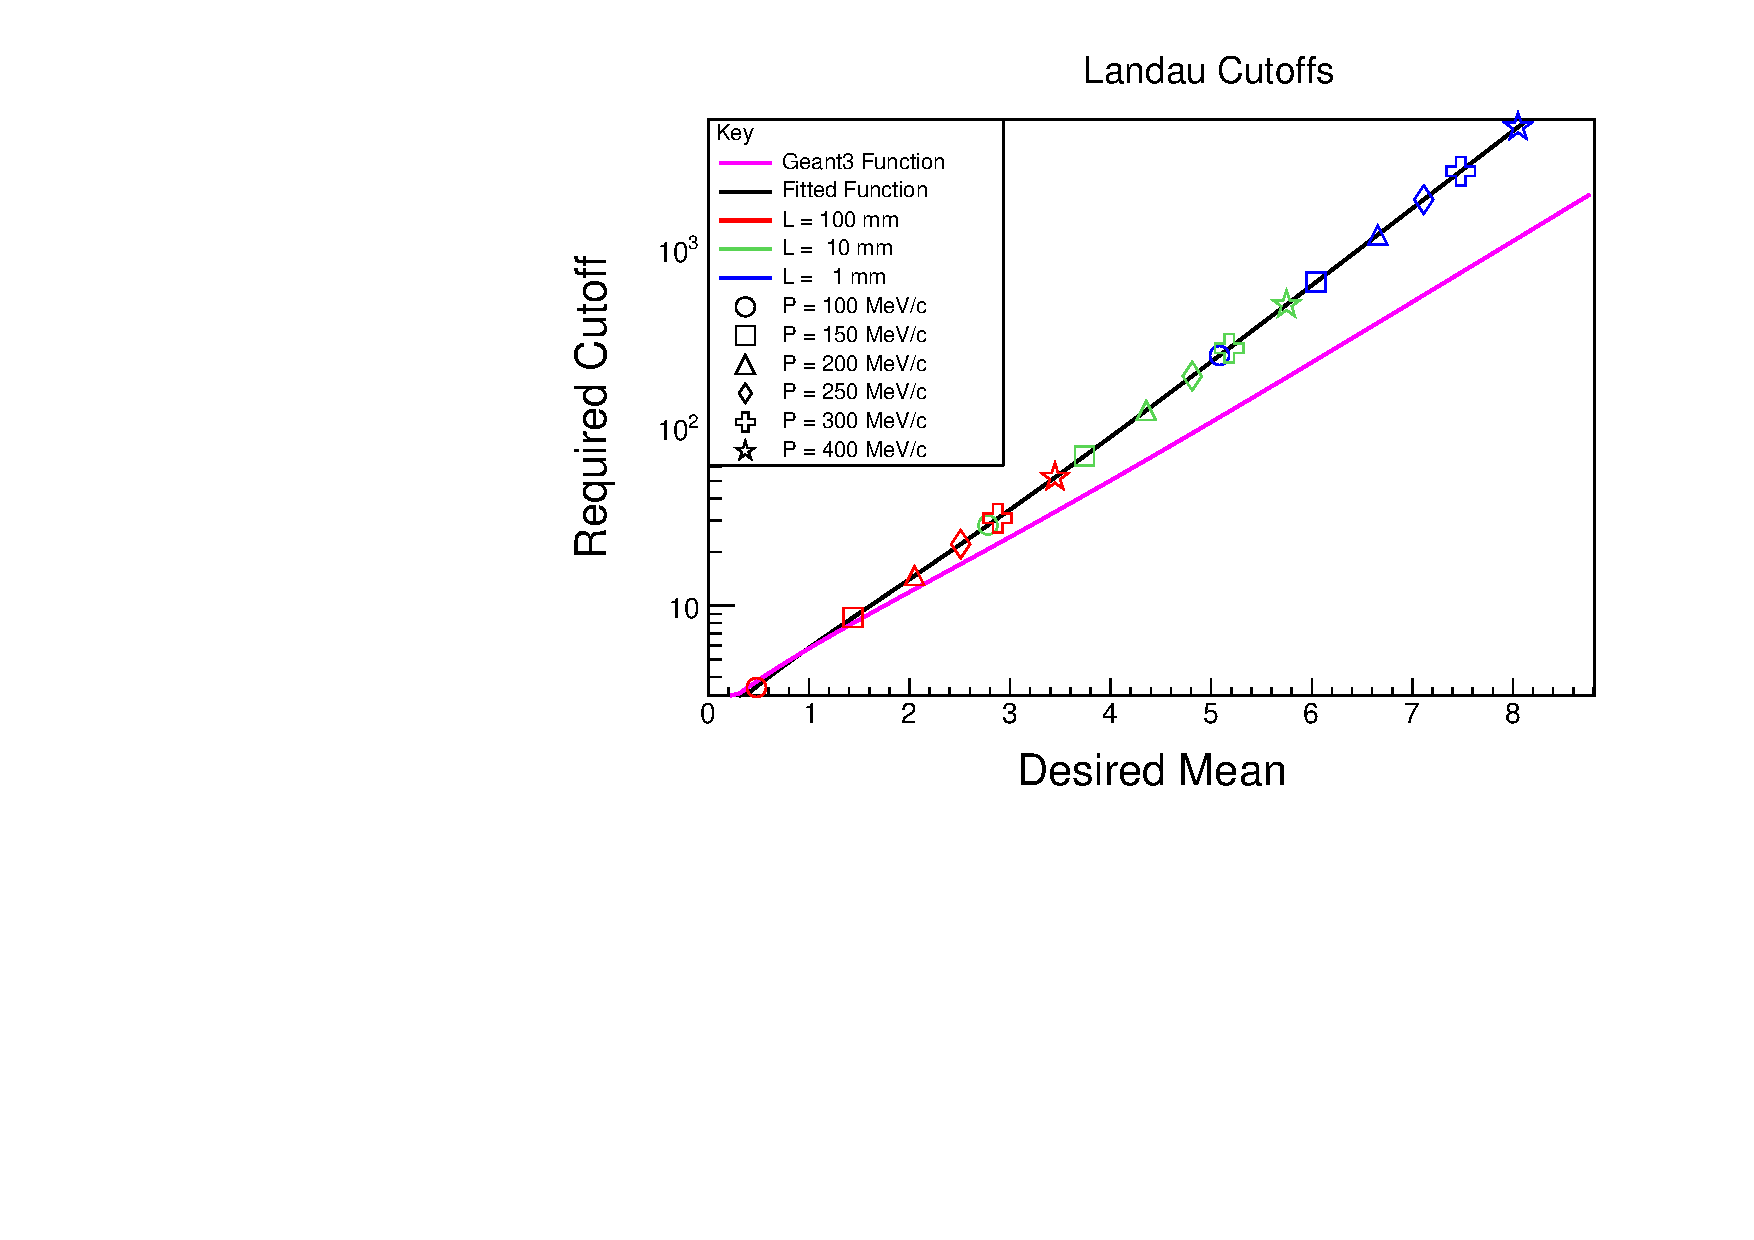
\includegraphics[width=\textwidth]{Figures/landau_cutoffs} 
  \caption[$\lambda_{max}$ vs. $\left<\lambda\right>$ over a variety of liquid hydrogen absorber lengths and initial beam momenta.]{$\lambda_{max}$ vs. $\left<\lambda\right>$ over a variety of liquid hydrogen absorber lengths and initial beam momenta. The pink line is the form given by GEANT3 (see Eq. \eqref{eqn:landauCutoffsGeant3}) and the black line is the fitted curve (see Eq. \eqref{eqn:landauCutoffs}). The data points are combinations of shapes and colors, as seen in the key. For example, since green means 10 mm and the square means 150 MeV/$c$, the green square data point represents the required cutoff for 150 MeV/$c$ muons passing through 10 mm of liquid hydrogen. Liquid hydrogen was chosen in order to match the results in Section~\ref{sec:benchmark}. However, other materials (such as lithium hydride) still fall within the desired $\left<\lambda\right>$ range of [0, 9].}
  \label{fig:landau_cutoffs}
\end{figure}

Based on Eq. \eqref{eqn:landauParameter}, it is possible to find $\epsilon_{max}$:
\begin{align*}
\epsilon_{max}=\xi[\lambda_{max}+(1-C_{Euler})+\beta^2+\ln(\xi/T_{max})]+\left<\epsilon\right>.
\end{align*}
Therefore, during the energy loss sampling, if any energy loss $\epsilon$ is selected which is greater than $\epsilon_{max}$ it is discarded and the sampling is performed again. However, if the result has been discarded 100 times, the particle is assumed to have lost too much energy and is considered lost.

%
%-------------------------------------------------------------------------------
%
\Section{Multiple Scattering in COSY Infinity} \label{sec:COSYScattering}\par
Similar to ICOOL's fifth model of scattering, the Rutherford model (see Section~\ref{sec:ICOOLScattering}), COSY utilizes a piecewise distribution function which is Gaussian  at small angles (as Goudsmit and Saunderson suggested \cite{gs}) and Rutherford-like at large angles. This Rutherford-like tail is derived at length in Appendix~\ref{apx:cosy_cross_section}, with a review of the relevant particle physics symbols and methods in Appendix~\ref{apx:particlePhysicsReview}. The result is the (differential) Mott scattering cross section:
\begin{equation}\label{eqn:MottCrossSection}
\frac{d\sigma}{d\Omega} \propto \frac{1+\frac{(\beta\gamma)^2}{2} (1+\cos\theta)  }{(1-\cos\theta)^2},
\end{equation}
where $d\sigma/d\Omega$ is the differential scattering cross section, $\beta$ is the velocity in units of $c$, $\gamma=1/\sqrt{1-\beta^2}$, and $\theta$ is the scattering angle. Observe that for the non-relativistic limit $\beta\rightarrow 0$ the cross section does indeed approach a Rutherford distribution (Eq. \eqref{eqn:rutherford}). The practical implementation of this cross section into the probability distribution function is discussed in Section~\ref{ssc:COSYScatteringImplementation}.

\Subsection{Implementation}\label{ssc:COSYScatteringImplementation} Now that the forms of the Gaussian and Rutherford-like scattering cross sections have been obtained, implementation of these cross sections is discussed. In this work, when a particle passes through matter, the change in angle of this particle is selected from a probability distribution. For $u=\cos\theta$, this distribution should be Gaussian-like at small angles \cite{gs} and follow the Mott cross section at large angles. Based on a Gaussian-like cross section for small angles and the cross section in Eq. \eqref{eqn:MottCrossSection}, the distribution has been chosen as
\begin{align}\label{eqn:cosyg}
g(u)=	\begin{dcases}
	e^{-a(1-u)} & \quad u_0 \leq u \\
	\zeta\frac{1+\frac{1}{2}(\beta\gamma)^2(1+u-b_c)}{(1-u+b_c)^2} & \quad u\leq u_0
	\end{dcases},
\end{align}
where $u_0$ is the cutoff between the Gaussian-like distribution and the Mott distribution, $\zeta$ is the amplitude of the Mott distribution, and $b_c$ is the relative $u$ shift of the Mott distribution. The parameter $a$ is an empirical parameter, based on Highland theory \cite{highland}, and can be found in Eq. \eqref{eqn:geanta}. Eq. \eqref{eqn:geanta} is reproduced here for convenience:
\begin{align*}
a=\frac{0.5}{1-\cos\theta_0},
\end{align*}
where $\theta_0$ has the form \cite{highland} 
\begin{align*}
\theta_0 = \frac{E_s}{p\beta} \sqrt{\frac{L}{X_0}}.
\end{align*}
However, this definition has been extended in this work to include empirical corrections based on GEANT4's \cite{geant4} treatment of $\theta_0$ (see Eq. \eqref{g4bltheta0}):
\begin{equation}\label{eqn:cosytheta0}
\theta_0 = \frac{13.6 \text{ eV}}{\beta p} \sqrt{\frac{L}{X_0} \left[ 1+h_1 \ln \frac{L}{X_0} + h_2 \left(\ln \frac{L}{X_0}\right)^2 \right] }.
\end{equation}
The Highland correction terms have been chosen novelly in this work as $h_1=0.12$ and $h_2=0.006$. This was done by fitting the curve given by Eq. \eqref{eqn:cosyg} to match the MuScat results \cite{muscat}, the results of which can be found in Section~\ref{sec:validation}. It is important to note that these correction terms are tunable for future data based on muons traversing higher $Z$ material.

$u_0$ is the point at which the Gaussian term meets the Mott tail. This has been chosen empirically as
\begin{equation}\label{eqn:cosyu0}
u_0=1-\frac{4.5}{a}.
\end{equation}
This parameter was fitted alongside the Highland correction terms to match the experimental results in \cite{muscat}.

$\zeta$ and $b_c$ are the angular scattering distribution's amplitude and offset for the tail. These are found by demanding continuity and smoothness at $u_0$:
\begin{align*}
e^{-a(1-u_0)}&=\zeta\frac{1+\frac{1}{2}(\beta\gamma)^2(1+u_0-b_c)}{(1-u_0+b_c)^2},\\
ae^{-a(1-u_0)}&=\zeta\frac{1+\frac{1}{2}(\beta\gamma)^2(1+u_0-b_c)}{(1-u_0+b_c)^2} \left(\frac{2}{1-u_0+b_c}+\frac{(\beta\gamma)^2}{2+(\beta\gamma)^2(1+u_0-b_c)}\right).
\end{align*}
Then
\begin{align*}
a=\frac{2}{1-u_0+b_c}+\frac{(\beta\gamma)^2}{2+(\beta\gamma)^2(1+u_0-b_c)}.
\end{align*}
Solving this for $(u_0-b_c)$ yields a quadratic with the solution
\begin{align} \label{eqn:cosybc}
b_c=u_0+\frac{A_2 + \sqrt{A_2 ^2 - 4A_1 A_3}}{2A_1},
\end{align}
with
\begin{align*}
A_1=&-a(\beta\gamma)^2,\\
A_2=&-(\beta\gamma)^2-2a,\\
A_3=&(\beta\gamma)^2(a-3)+2a-4.
\end{align*}
The continuity condition for $g(u_0)$ yields the expression for $\zeta$:
\begin{equation}\label{eqn:cosyzeta}
\zeta=\frac{e^{-a(1-u_0)}(1-u_0+b_c)^2}{1+\frac{1}{2}(\beta\gamma)^2(1+u_0-b)}.
\end{equation}

Now that the distribution function has a concrete form, it is implemented by inverting the cumulative distribution function (CDF).  Let $G(u)$ be the integral of $g(u)$. Then the variable $G$ is uniformly sampled over the region $[0,G_{max}]$. If $G\geq G(u_0) \equiv G_0$ then the Gaussian part of the distribution is used to generate $u$ (i.e., $G(u\geq u_0)$). Otherwise, the tail of the CDF is used. Figure~\ref{fig:scatdist_example} shows $G(u)$ for $L=100$ mm, $p=200$ MeV/$c$, and a radiation length $X_0 = 8.66$ m (to simulate a liquid hydrogen target).\footnote{The value of 8.66 m as the radiation length of liquid hydrogen was chosen so that it matches the value found in the ICOOL source files. This differs from the radiation length of liquid hydrogen found in the PDG website \cite{PDG}, which is 8.904 m.}

\begin{figure}
  \centering
    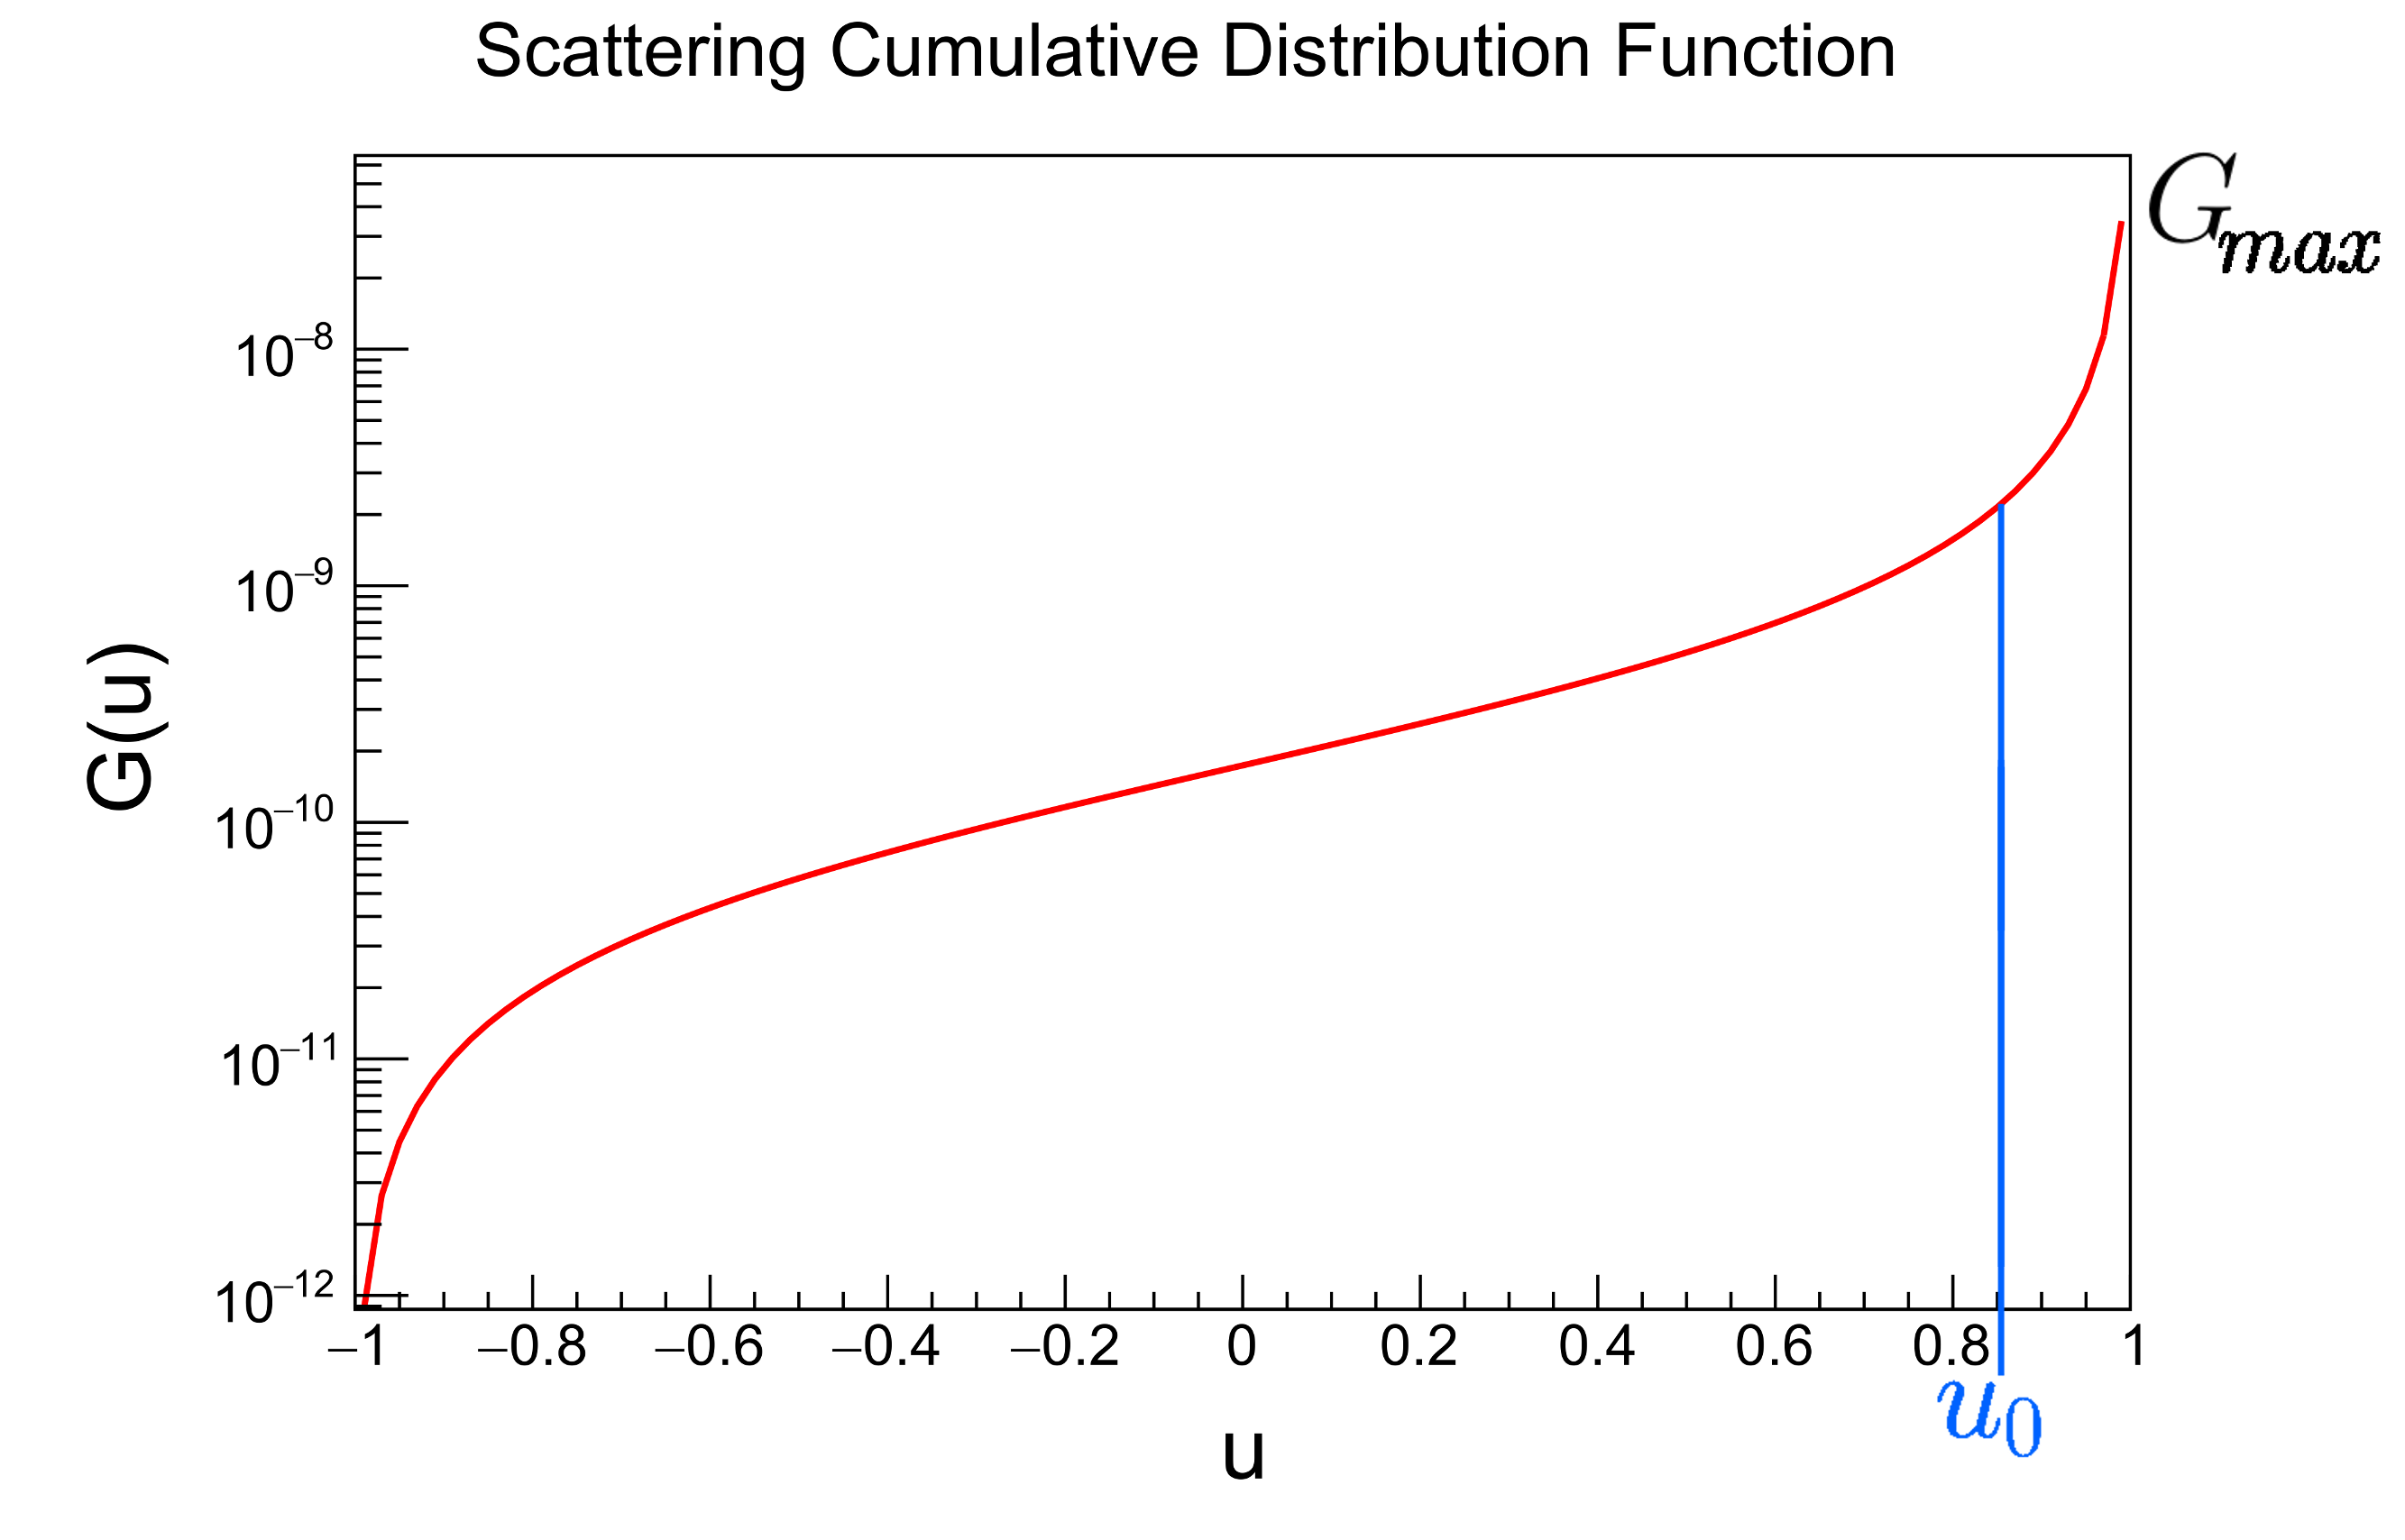
\includegraphics[width=\textwidth]{Figures/scatdist_example} 
  \caption[Example of the COSY cumulative angular distribution function.]{Example of the cumulative angular distribution function for muons with momenta of 200 MeV/$c$ passing through 100 mm of liquid hydrogen. Note that the $y$ axis is log scaled due to the very sharp peak. Furthermore, note that $u_0$ is greatly exaggerated, since its actual value for these parameters is 0.99987.}
  \label{fig:scatdist_example}
\end{figure}

However, since this is a piecewise function, the CDF is inverted in pieces. The tail of the CDF is found first:
\begin{align*}
G(u\leq u_0)=\int _{-1} ^u \zeta \frac{1+\frac{1}{2}(\beta\gamma)^2 (1+u'-b_c)}{(1-u'+b_c)^2} du'.
\end{align*}
This integral may be solved by substituting $v=1-u'+b_c$ and simply splitting the numerator into separate parts:
\begin{align}
\nonumber
G(u\leq u_0)=&-\zeta(1+\frac{1}{2}(\beta\gamma)^2(1-b_c))\int_{2+b_c} ^{1-u+b_c} v^{-2} dv - \\
\nonumber
& \quad \zeta \frac{(\beta\gamma)^2}{2}\int_{2+b_c} ^{1-u+b_c} (v^{-2} - v^{-1} + b_c v^{-2}) dv,\\
G(u\leq u_0)=&\zeta(1+(\beta\gamma)^2)\left(\frac{1}{1-u+b_c} - \frac{1}{2+b_c}\right)+\zeta \frac{(\beta\gamma)^2}{2} \ln\left(\frac{1-u+b_c}{2+b_c}\right). \label{eqn:cosyGTail}
\end{align}

The goal is to solve Eq. \eqref{eqn:cosyGTail} for $u(G)$. However, using direct inversion is extremely difficult and involves special functions. Therefore, it is more prudent to generate  $u$ via bisection method (see Figure~\ref{fig:scatdist_algorithm}). In this method, the true $G$ is sampled uniformly on the range $[0,G_{max}]$, where $G_{max} \equiv G(1)$. Explicitly, $G_{max}$ is
\begin{align*}
G_{max}\equiv G(1) &=\int_{-1} ^{u_0} \zeta\frac{1+\frac{1}{2}(\beta\gamma)^2(1+u-b_c)}{(1-u+b_c)^2}du+\int_{u_0} ^1 e^{-a(1-u)} du,\\
&= G_0+\frac{1}{a}-\frac{e^{-a(1-u_0)}}{a}.
\end{align*}
If $G < G_0$, then the tail is sampled. A trial $u$ called $\bar{u}$ (as in ``average'') is selected from some range which is known to contain the actual $u$. The range is described as $[u_{min},u_{max}]$, and $\bar{u}=(u_{min}+u_{max})/2$. 

Initially, the range is chosen as $u_{min}=-1$ and $u_{max}=u_0$ (since that is the largest range on which $G(u \leq u_0)$ is valid and hence $u$ is guaranteed to be in this range). $\bar{G} \equiv G(\bar{u})$ is found using Eq. \eqref{eqn:cosyGTail}, and then the routine is subject to the following conditions:
\begin{align*}
&\text{If } \bar{G}\in [G-\delta G,G+\delta G] &\quad &\text{then } u=\bar{u}\text{, return value.}\\
&\text{If } \bar{G} < G-\delta G &\quad &\text{then } u_{min}=\bar{u} \text{, rerun with new }u_{min}.\\
&\text{If } \bar{G} > G+\delta G &\quad &\text{then } u_{max}=\bar{u} \text{, rerun with new }u_{max}.
\end{align*}
$\delta G$ is a precision, and has been chosen for this work as $\delta G = 10^{-8}$. However, it is conceded that in the future $\delta G$ should be a percentage of $G_{max}$ rather than an absolute number.

\begin{figure}
  \centering
    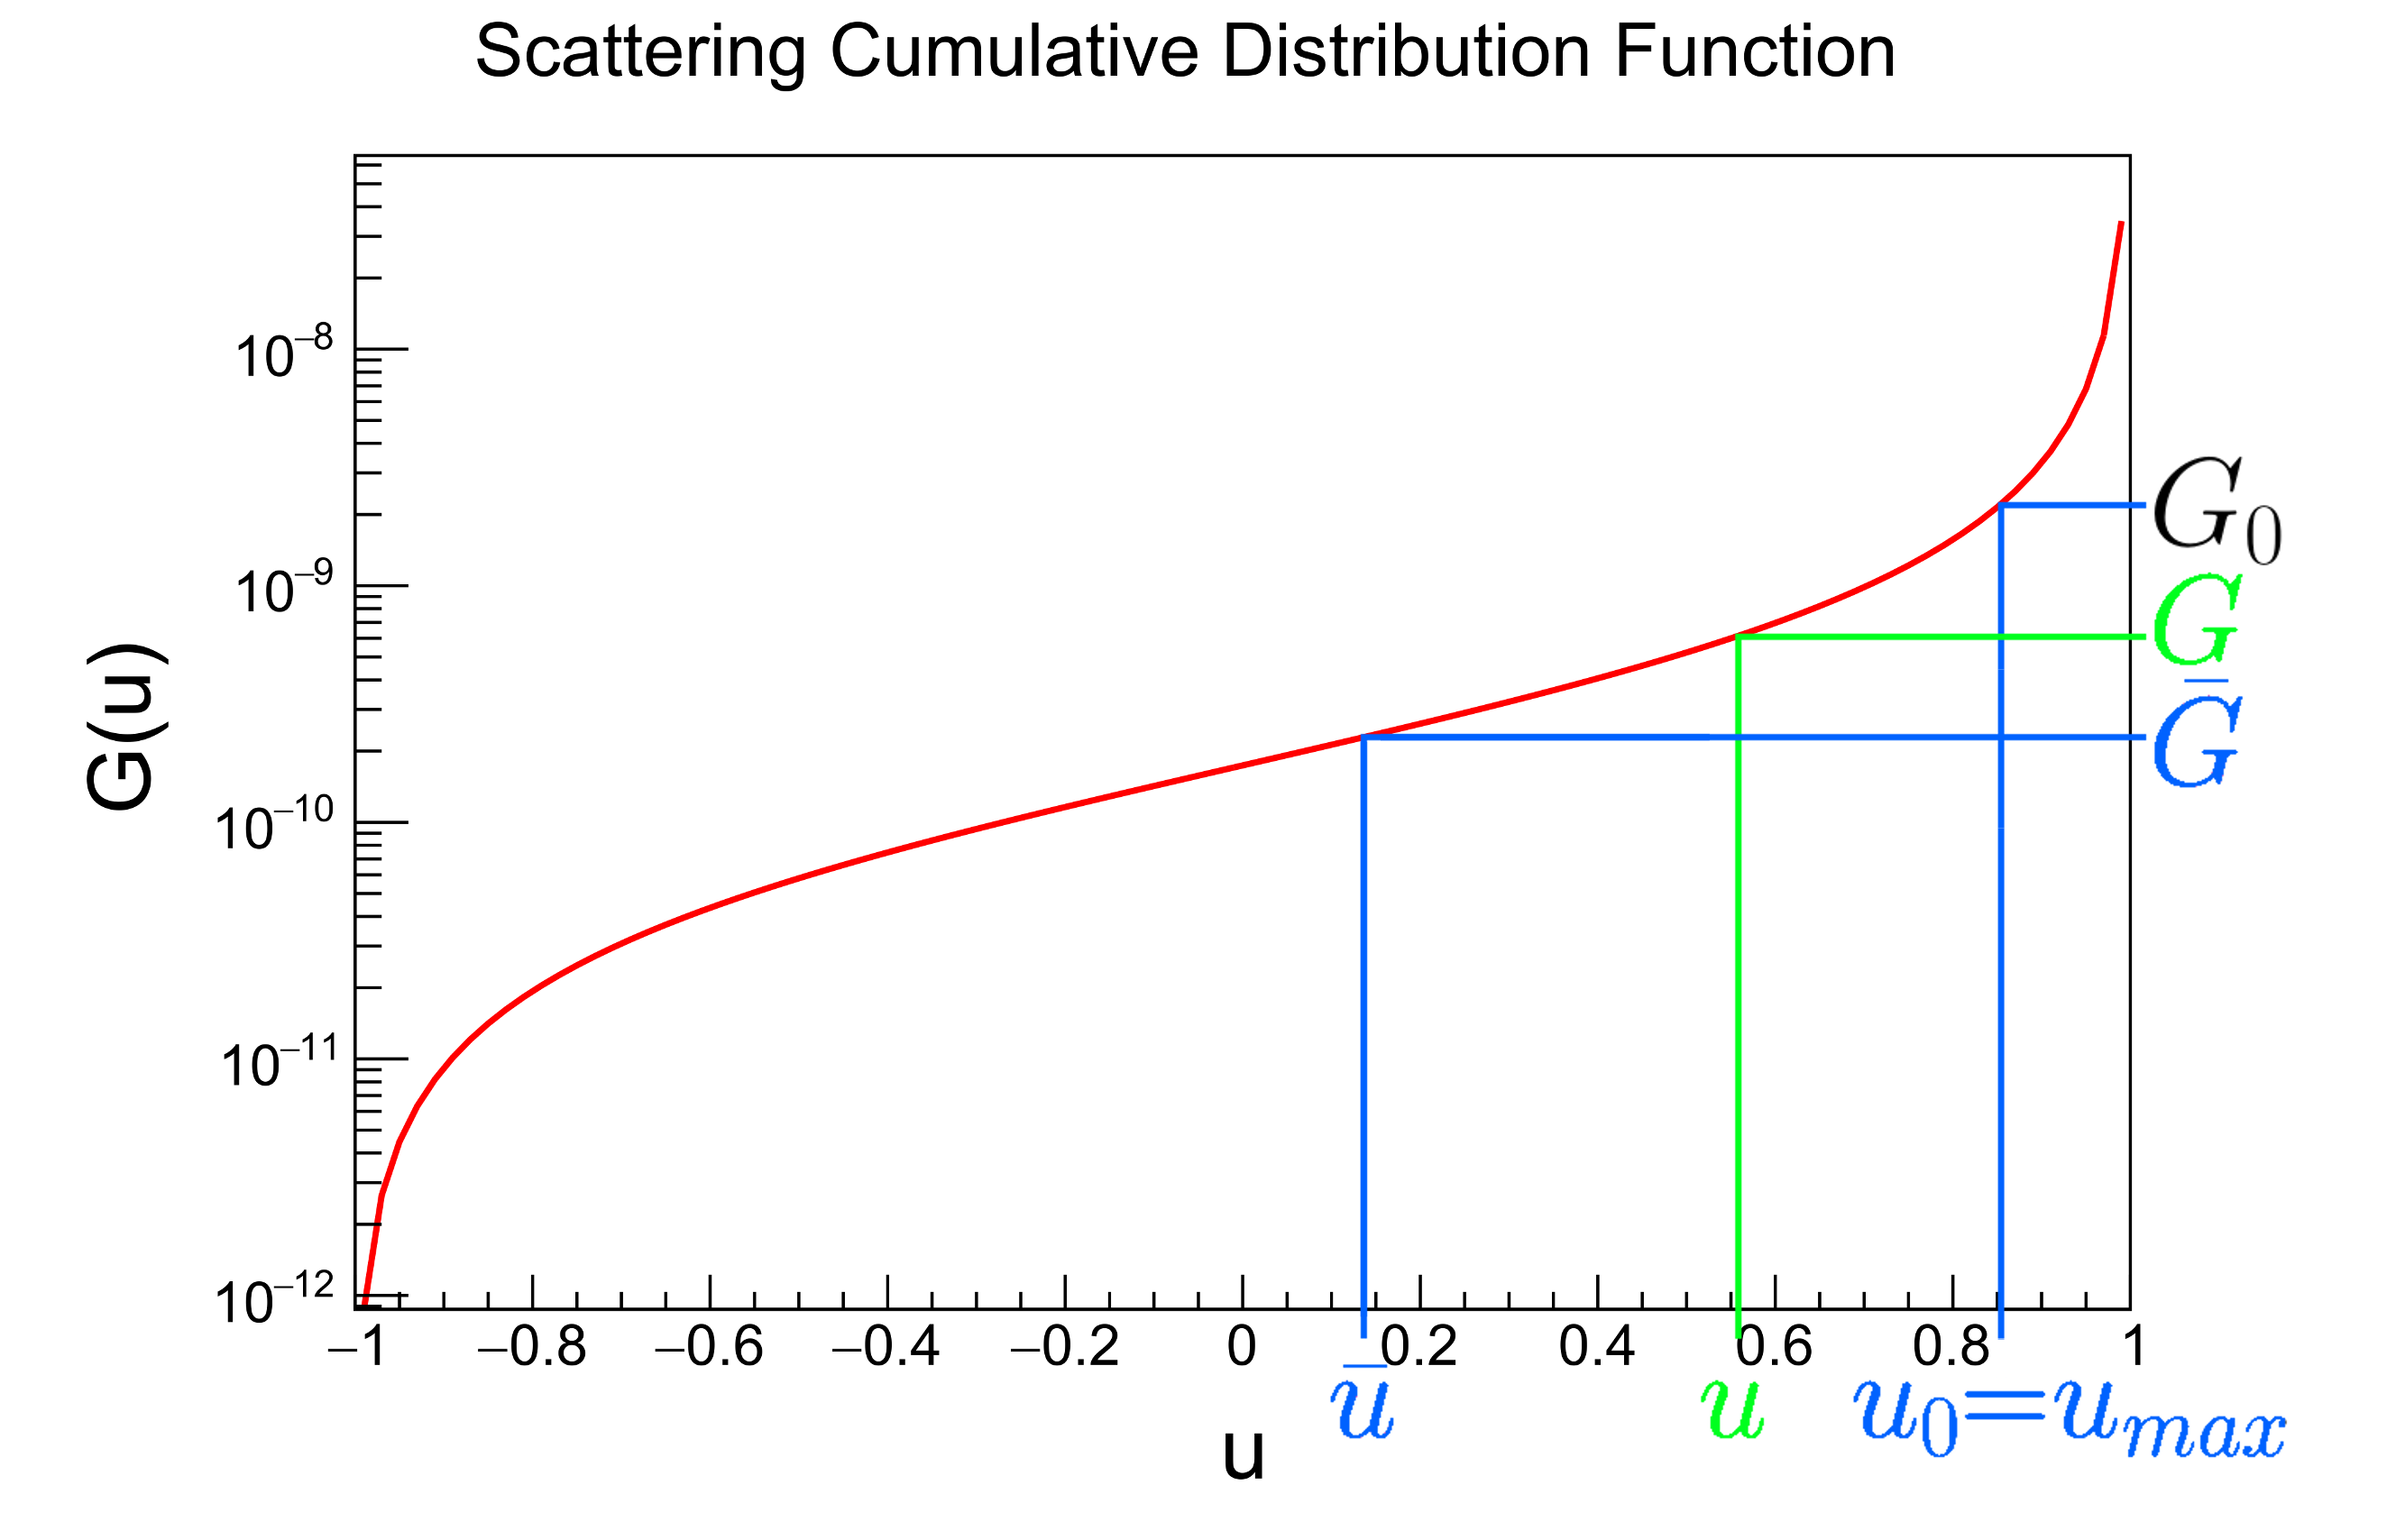
\includegraphics[width=\textwidth]{Figures/scatdist_algorithm} 
  \caption[Example of the first iteration of the COSY CDF algorithm.]{Example of the first iteration of the algorithm to obtain the true $u$ (in green). The true $G$ is chosen uniformly from $G\in[0,G_{max}]$. If $G < G_0$, then the tail is sampled via bisection method. In this case, since $\bar{G} < G$, $\bar{u}$ is the new $u_{min}$ and $\bar{u}$ is calculated again.}
  \label{fig:scatdist_algorithm}
\end{figure}

For the peak, $u_0 \leq u$ and so the CDF becomes
\begin{align*}
G(u_0 \leq u)&=\int_{-1} ^{u_0} g(u) du + \int_{u_0} ^u e^{-a(1-u)} du.
\end{align*}
The first term is simply $G_0$, the cumulative distribution function at $u_0$. The second term is easily integratable and yields
\begin{equation}\label{eqn:cosyGPeak}
G(u_0 \leq u)=G_0 + \frac{e^{-a(1-u)}-e^{-a(1-u_0)}}{a}.
\end{equation}
The inversion of this function is quite straightforward, and is
\begin{equation} \label{eqn:cosyGPeakInverted}
u(G_0 \leq G)=1+\frac{1}{a} \ln \left[a(G-G_0)+e^{-a(1-u_0)}\right].
\end{equation}
Therefore, if $G \in [0,G_{max}]$ is greater than or equal to $G_0$, then it is simply inserted into Eq. \eqref{eqn:cosyGPeakInverted} and the true $u$ is obtained.

It is a subtle yet important point to note that the Mott cross section (Eq. \eqref{eqn:MottCrossSection}), upon which the probability distribution function $g(u)$ in Eq. \eqref{eqn:cosyg} is based, assumes an on-axis straight line trajectory. An on-axis trajectory is equivalent to saying that $p_z=p$ and $x=y=p_x = p_y =0$. For particles that are not on-axis, the reference frame both before and after scattering is rotated such that $p=p_z$. A particle that is not on-axis is exemplified in Figure~\ref{fig:cosyRotatedFrame}. Here, the muon has some angle $\theta_o$ before entering the medium. The lab frame has transverse and longitudinal position axes $T$ and $z$ and the rotated frame has corresponding transverse and longitudinal position axes $T_R$ and $z_R$.  

\begin{figure}
  \centering
    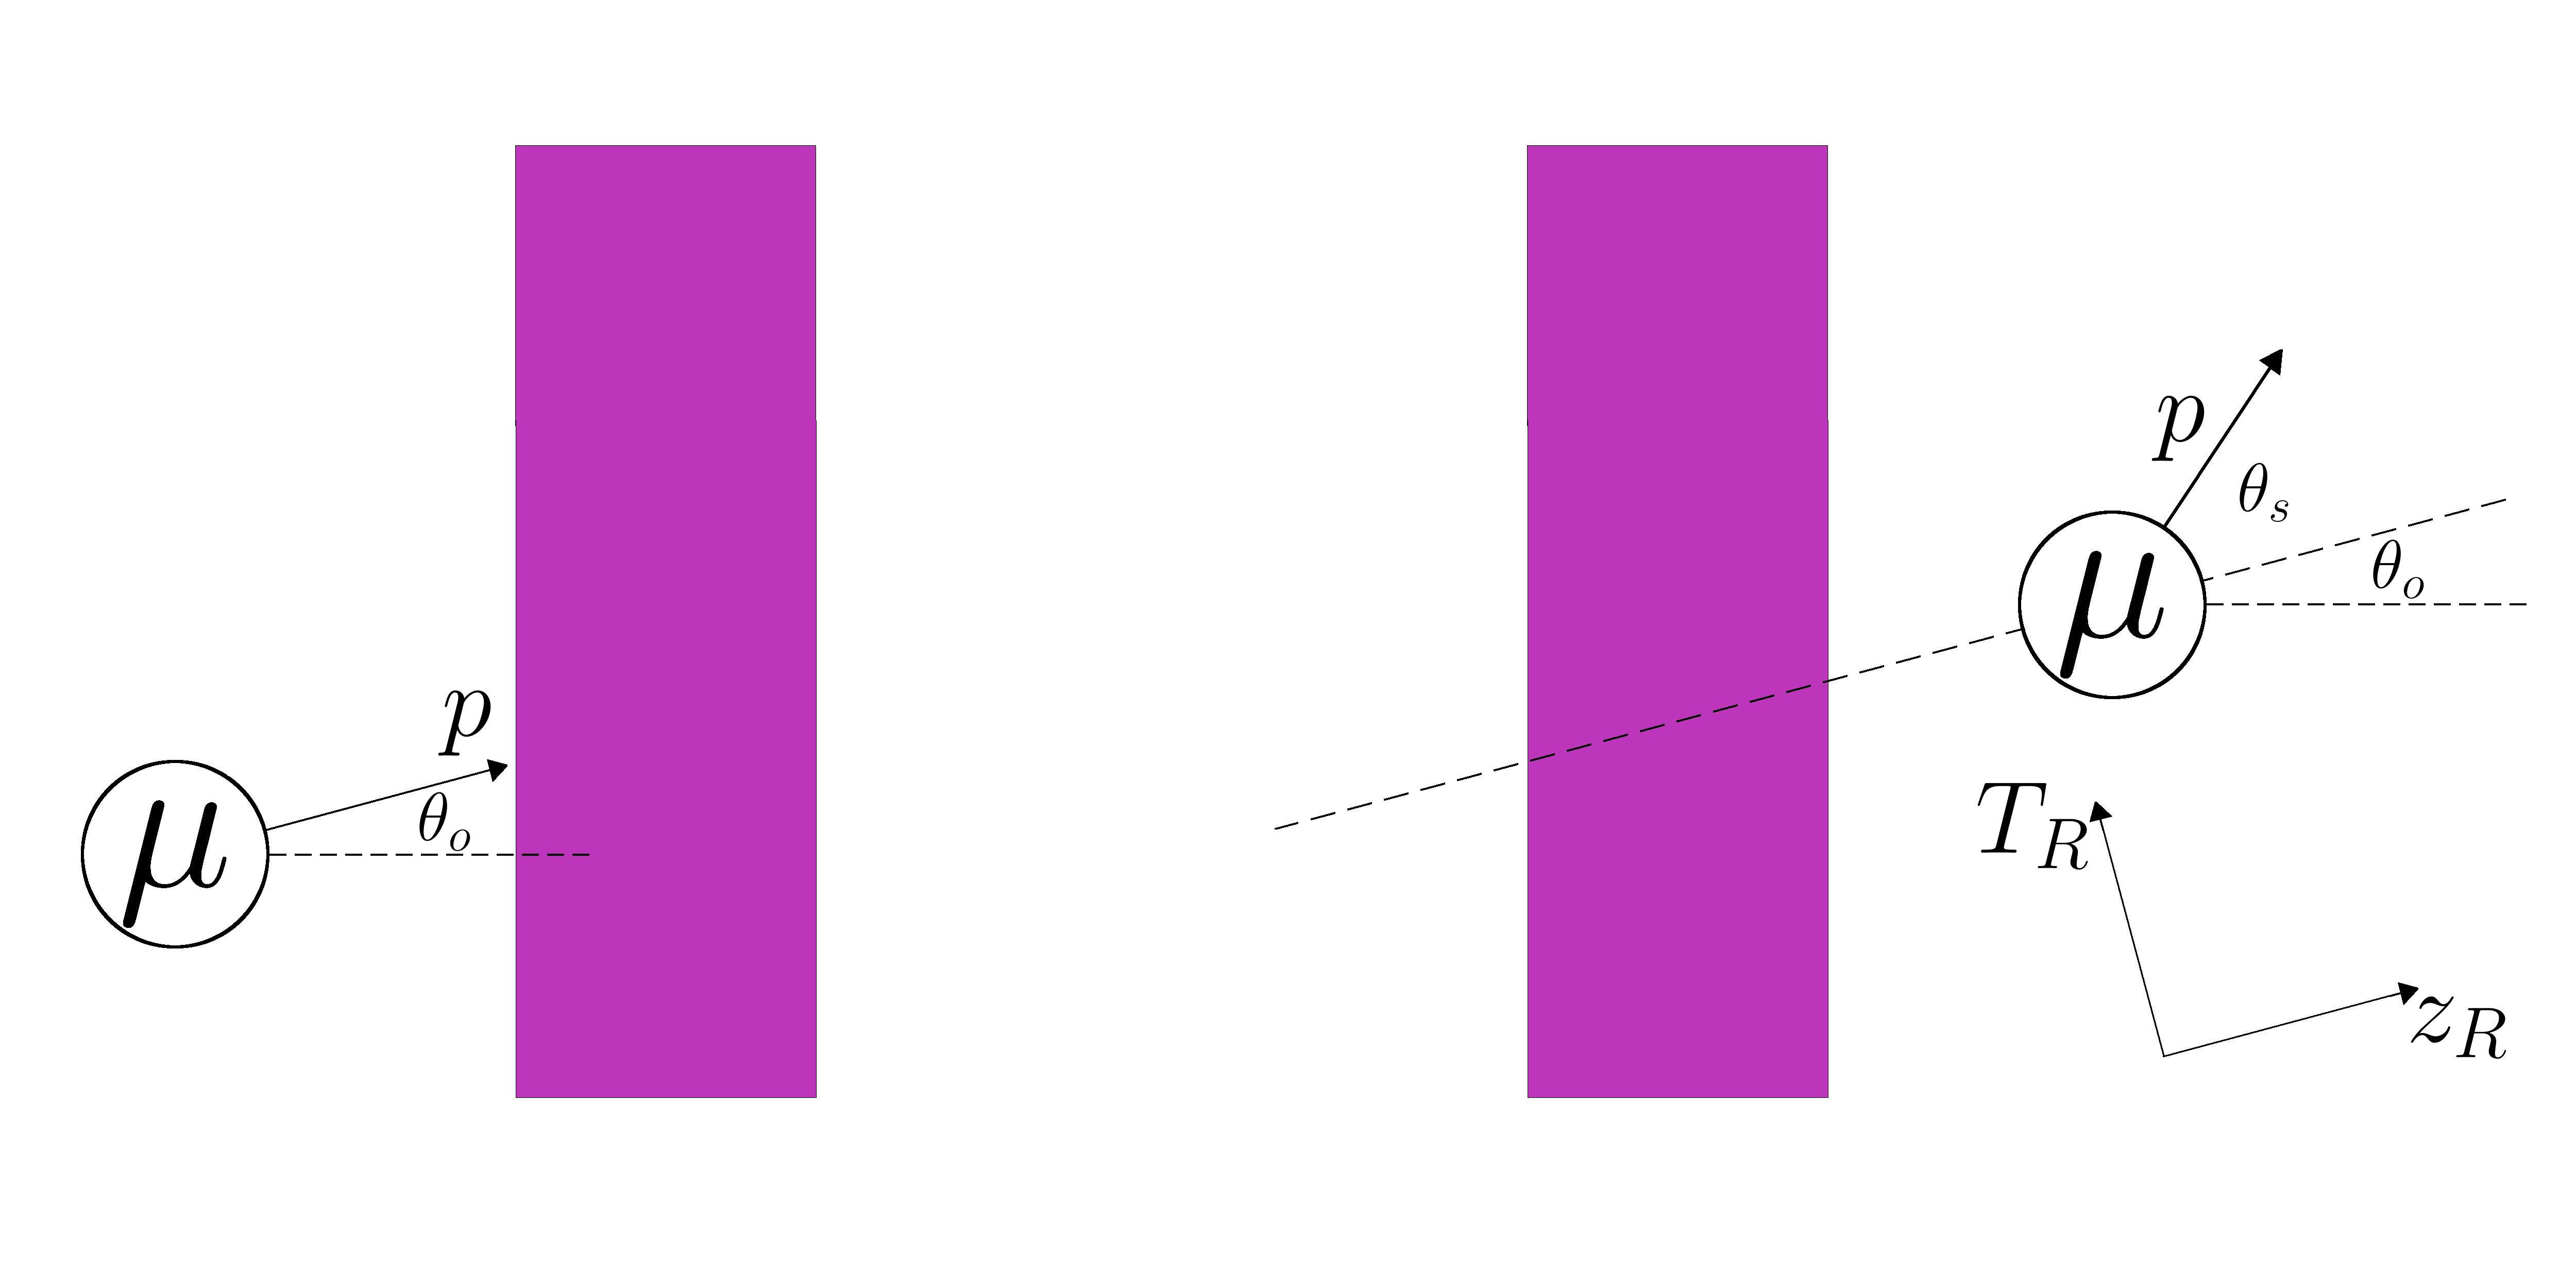
\includegraphics[width=\textwidth]{Figures/cosyRotatedFrame} 
  \caption[Example of a muon entering an absorber with some nonzero initial angle.]{Example of a muon entering an absorber (purple) with some nonzero initial angle $\theta_o$. The muon then scatters an angle $\theta_s$ with respect to its inital momentum $\vec{p}$. The scattering distribution $g(u)$ assumes a straight, on-axis particle ($x=y=p_x=p_y=0$) before scattering, and so is in the rotated frame represented by $T_R, z_R$.}
  \label{fig:cosyRotatedFrame}
\end{figure}

To reiterate, prior to scattering, in the rotated frame the rotated longitudinal momentum is the total momentum ($p_{z,R}=p$) and the rotated transverse momentum is zero ($p_{T,R}=0$). After scattering, $g(u)$ yields the scattered angle $\theta_s$. The rotated longitudinal momentum is no longer necessarily equal to the total momentum, but rather $p_{z,R}=p\cos\theta_s$. Similarly, the rotated transverse momentum is not necessarily zero but instead $p_{T,R}=\sqrt{p^2-p_{z,R}}$. Note that since energy straggling has already been accounted for, the total momentum $p$ stays constant throughout the scattering process and regardless of reference frame.

Due to cylindrical symmetry, the transverse momentum in the rotated frame $p_{T,R}$ must be distributed uniformly into the transverse $x$ and $y$ momenta. The constraint upon the transverse momentum in any frame is
\begin{align*}
p_T^2=p_x ^2+ p_y ^2.
\end{align*}
Therefore, the variable $\phi$ is selected uniformly from [0, 2$\pi$]. The $x$ and $y$ momenta in the rotated frame are
\begin{align*}
p_{x,R}&=P_{T,R}\cos\phi\cdot \text{sgn}(\phi-\pi),\\
p_{y,R}&=P_{T,R}\sin\phi,
\end{align*}
where sgn is the sign function defined by
\begin{align*}
\text{sgn}(x)=	\begin{cases}
		-1 &\qquad \text{for }x<0\\
		\ 0 &\qquad \text{for }x=0\\
		\ 1 &\qquad \text{for }x>0
		\end{cases}.
\end{align*}
The rotated $x$ and $y$ momenta ($p_{x,R}$ and $p_{y,R}$) are subsequently transformed into the lab frame. 
%The process of transforming the rotated scattering into lab coordinates may be found in Appendix~\ref{sec:fortran} on page \pageref{pg:scatdist}.
\iffalse





After energy straggling, the scattering routine which uses $g(u)$ is called.  This routine takes two arguments: $\theta_0$ (the Highland-like critical scattering angle from Eq. \eqref{eqn:cosytheta0}) and $p$, the total momentum. $\theta_0$ includes not only the dependence on material parameters ($L, X_0$) but also dependence on energy terms ($1/\beta p$). $p$ is the total momentum \textit{after} the straggling routine has been called.


The implemented routine for this work that uses the scattering distribution $g(u)$ is called \texttt{SCATDIST}. This routine takes two arguments: $\theta_0$ (the Highland-like critical scattering angle from Eq. \eqref{eqn:cosytheta0}) and $p$, the total momentum. $\theta_0$ includes not only the dependence on material parameters ($L, X_0$) but also dependence on energy terms ($1/\beta p$). $p$ is the momentum \textit{after} the straggling routine has been called. \texttt{SCATDIST} returns not the scattered angle, but the new $z$ momentum $p_z=pu=p\cos\theta$. 

This new $z$ momentum is in the rotated frame, i.e. the frame in which $p_x=p_y=0$ (see Figure~\ref{fig:cosyRotatedFrame}), and so is called $p_{z,R}$. The transverse momentum in the rotated frame, $p_{T,R}$, can be found via $p_{T,R}=\sqrt{p^2-p_{z,R}^2}$. The total transverse angle is $\theta_o + \theta_s$, which includes the original angle ($\theta_o$) and the transverse angle which was gained via scattering ($\theta_s$). Rotation back into the lab frame is given by
\begin{align*}
\begin{pmatrix}
p_{z} \\ p_T
\end{pmatrix}
=
\begin{pmatrix}
\cos\theta_o & -\sin\theta_o\\
\sin\theta_o & \cos\theta_o
\end{pmatrix}
\begin{pmatrix}
p_{z,R} \\ p_{T,R}
\end{pmatrix}.
\end{align*}

\begin{figure}
  \centering
    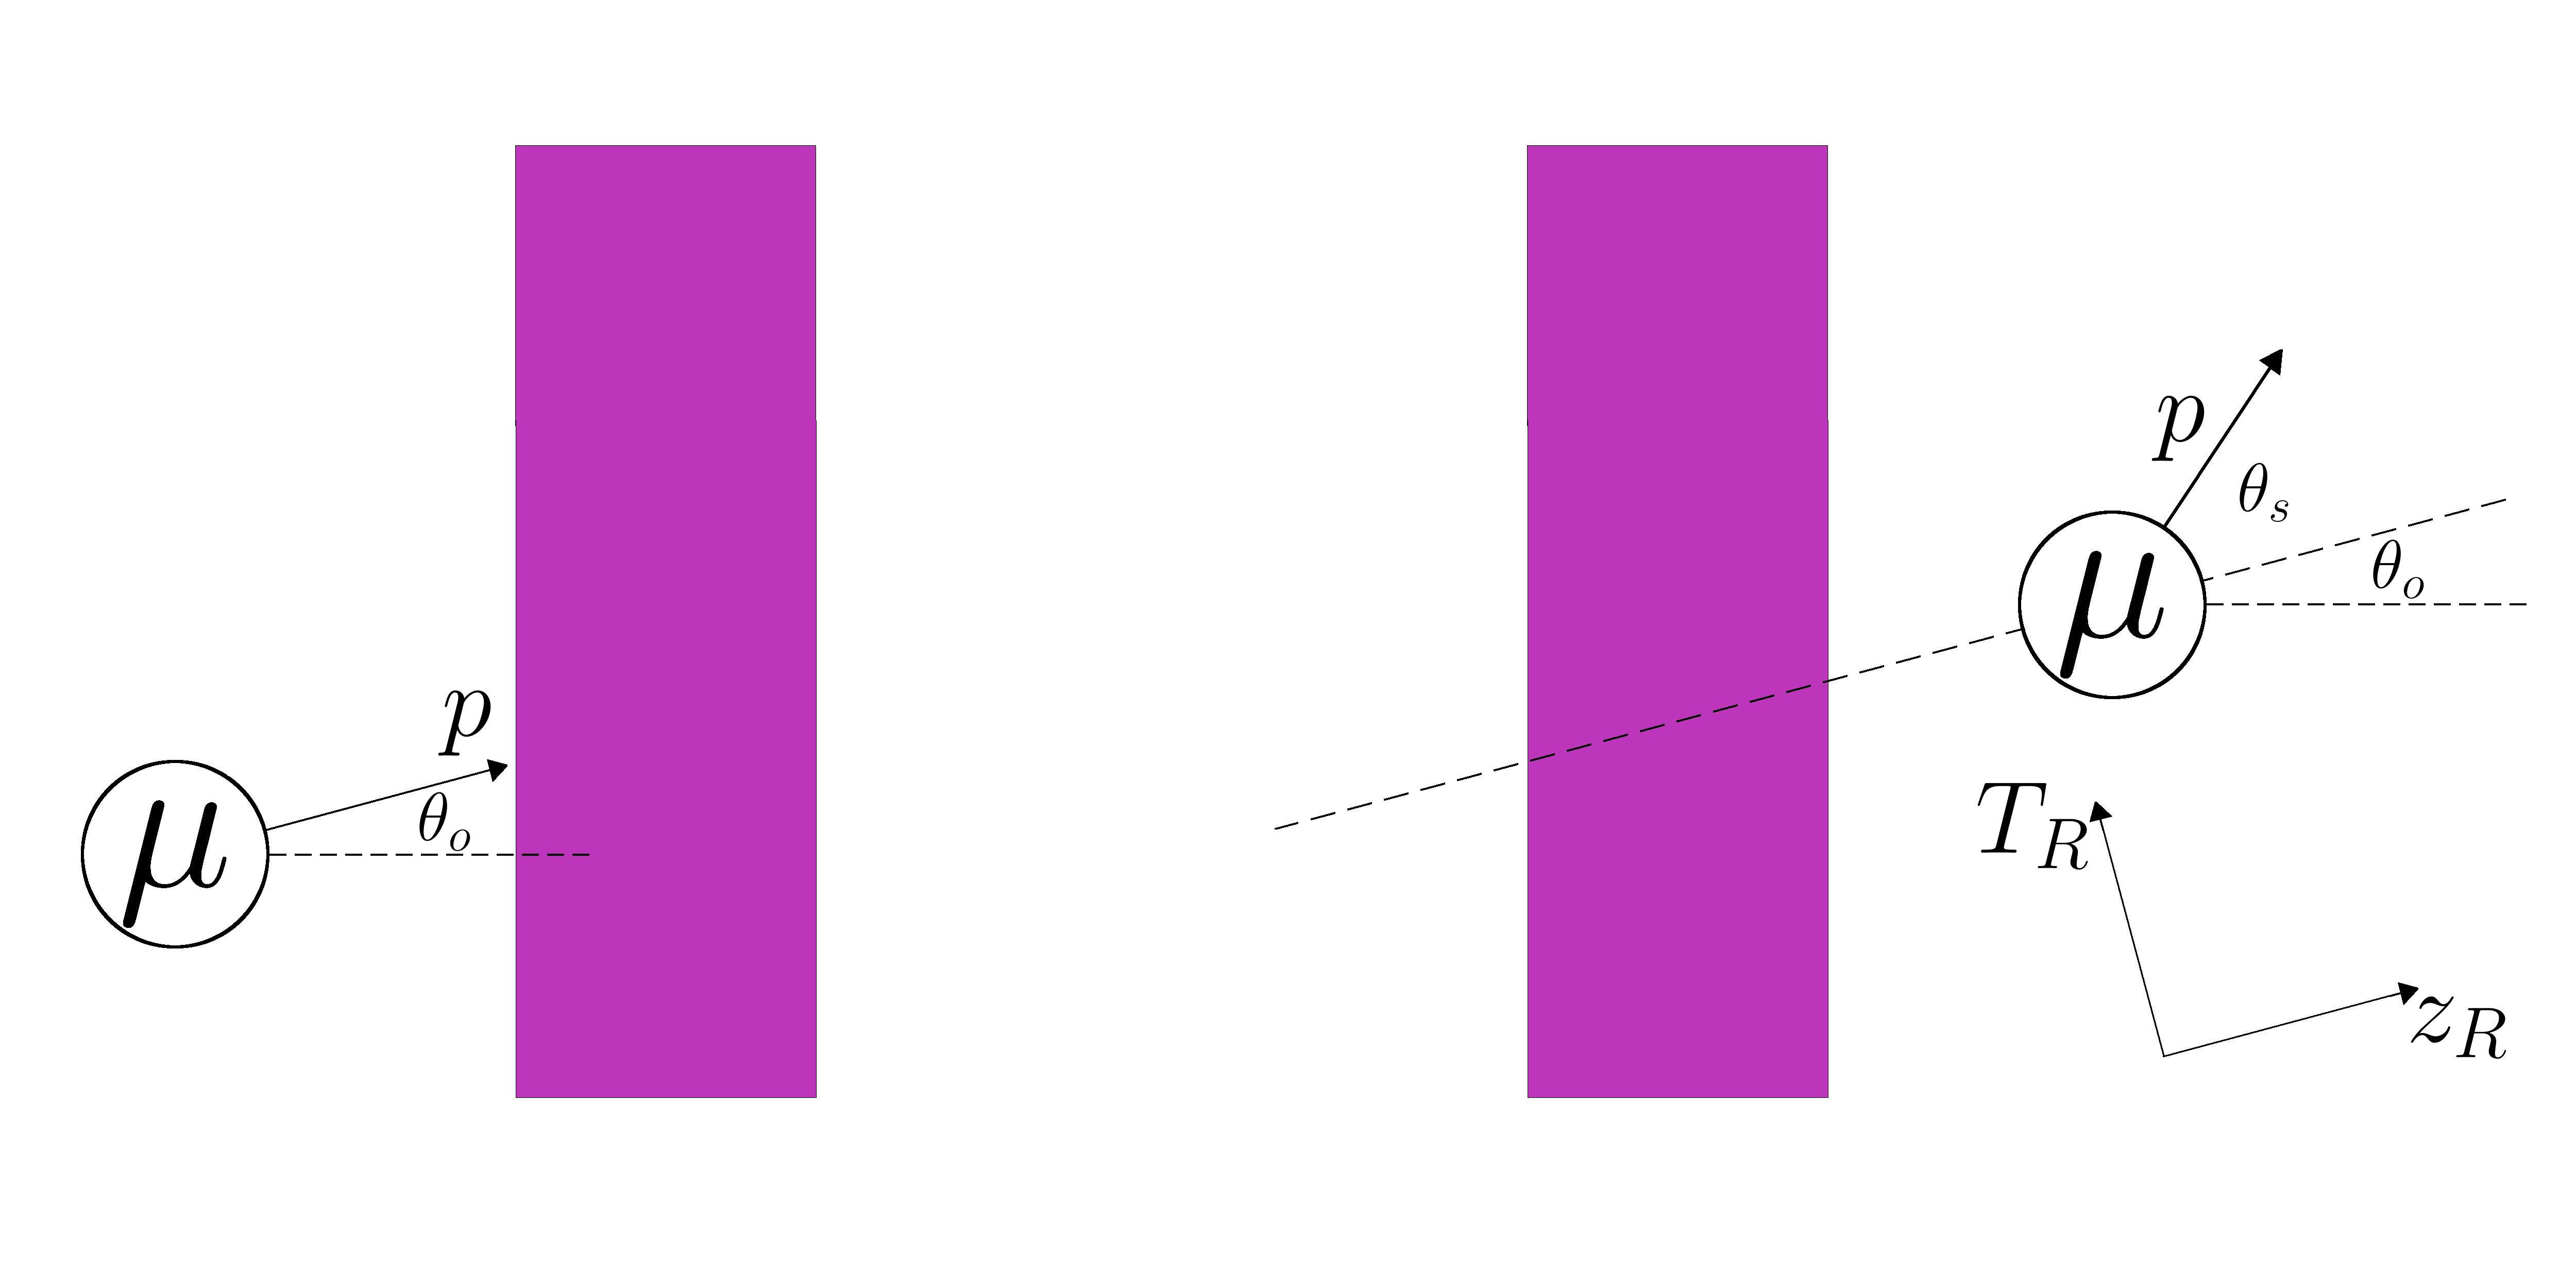
\includegraphics[width=\textwidth]{Figures/cosyRotatedFrame} 
  \caption[Example of a muon entering an absorber with some nonzero initial angle.]{Example of a muon entering an absorber (purple) with some nonzero initial angle $\theta_o$. The muon then scatters an angle $\theta_s$ with respect to its inital momentum $\vec{p}$. The scattering distribution $g(u)$ assumes a straight, on-axis particle ($x=y=p_x=p_y=0$) before scattering, and so is in the rotated frame represented by $T_R, z_R$.}
  \label{fig:cosyRotatedFrame}
\end{figure}

Note that at this point one must not uniformly distribute $p_T$ into $p_x$ and $p_y$. This is because, for example, if $p_x$ was positive before scattering it should have a strong probability of being positive after scattering. If one were to distribute $p_T$ uniformly then $p_x$ would have a 50/50 chance of being negative. For this reason, only the transverse momentum gained via scattering should be uniformly distributed into $p_x$ and $p_y$.

Let the original momenta (after straggling but before scattering) be denoted with the subscript $o$ in the same fashion that $\theta_o$ is the angle before scattering. Then the amount of transverse momentum which was gained via scattering is $P_T-P_{T,o}$. This new amount of transverse momentum must be added to the original $p_{x,o}$ and $p_{y,o}$ uniformly due to cylindrical symmetry. Consequently, let $\phi$ be an angle chosen from $[0,2\pi]$. Then the final $p_x$ and $p_y$ are
\begin{align*}
p_x&=p_{x,o}+(P_T-P_{T,o})\cos\phi\\
p_y&=p_{y,o}+(P_T-P_{T,o})\sin\phi.
\end{align*}







\fi

To summarize, the angular distribution used by COSY Infinity is based on a piecewise function which is Gaussian for small angles \cite{gs} and has a Mott tail for large angles. This distribution is represented by $g(u)$ in Eq. \eqref{eqn:cosyg}, where $u\equiv \cos\theta$. $g(u)$ has four parameters: $a$, an empirical parameter that is based on Highland theory \cite{highland} and is dependent on some critical angle $\theta_0$, defined in Eq. \eqref{eqn:cosytheta0}; $u_0$, the empirical cutoff angle that distinguishes which angles are Gaussian and which are not, found by Eq. \eqref{eqn:cosyu0}; $b_c$, a parameter derivable from smoothness of $g$ at $u_0$, which represents the offset of the Mott tail, found in Eq. \eqref{eqn:cosybc}; and $\zeta$, a parameter derivable from continuity of $g$ at $u_0$ which represents the amplitude of the Mott tail, found in Eq. \eqref{eqn:cosyzeta}. From $g(u)$, its antiderivative $G(u)$ may be found and a particular $G$ may be picked from the range $[0,G_{max}]$. If $G<G_0 \equiv G(u_0)$, then $u$ comes from the Mott tail and a bisection method is used to find $u$. If $G_0 \leq G$ then $u$ comes from the Gaussian peak and $G(u)$ may be inverted to find $u(G)$. This scattered angle must then be rotated into the lab frame and the additional transverse momentum must be uniformly distributed into $p_x$ and $p_y$.

%
%-------------------------------------------------------------------------------
%
\Section{Transverse Displacement in COSY Infinity}\label{sec:COSYTransverseDisplacement}\par
Due to multiple scattering events, when a particle traverses matter, a direct correlation between the particle transverse position and scattered angle is not always clear. Two identical particles with identical initial conditions may end up with identical scattered angles but different transverse positions (see Figure~\ref{fig:lateral_displacement}). This is because these two particles may take different paths through the absorber. While both of these paths may lead to a similar final angle with respect to the $z$ axis, the positions are likely different due to their trajectories.

\begin{figure}
  \centering
    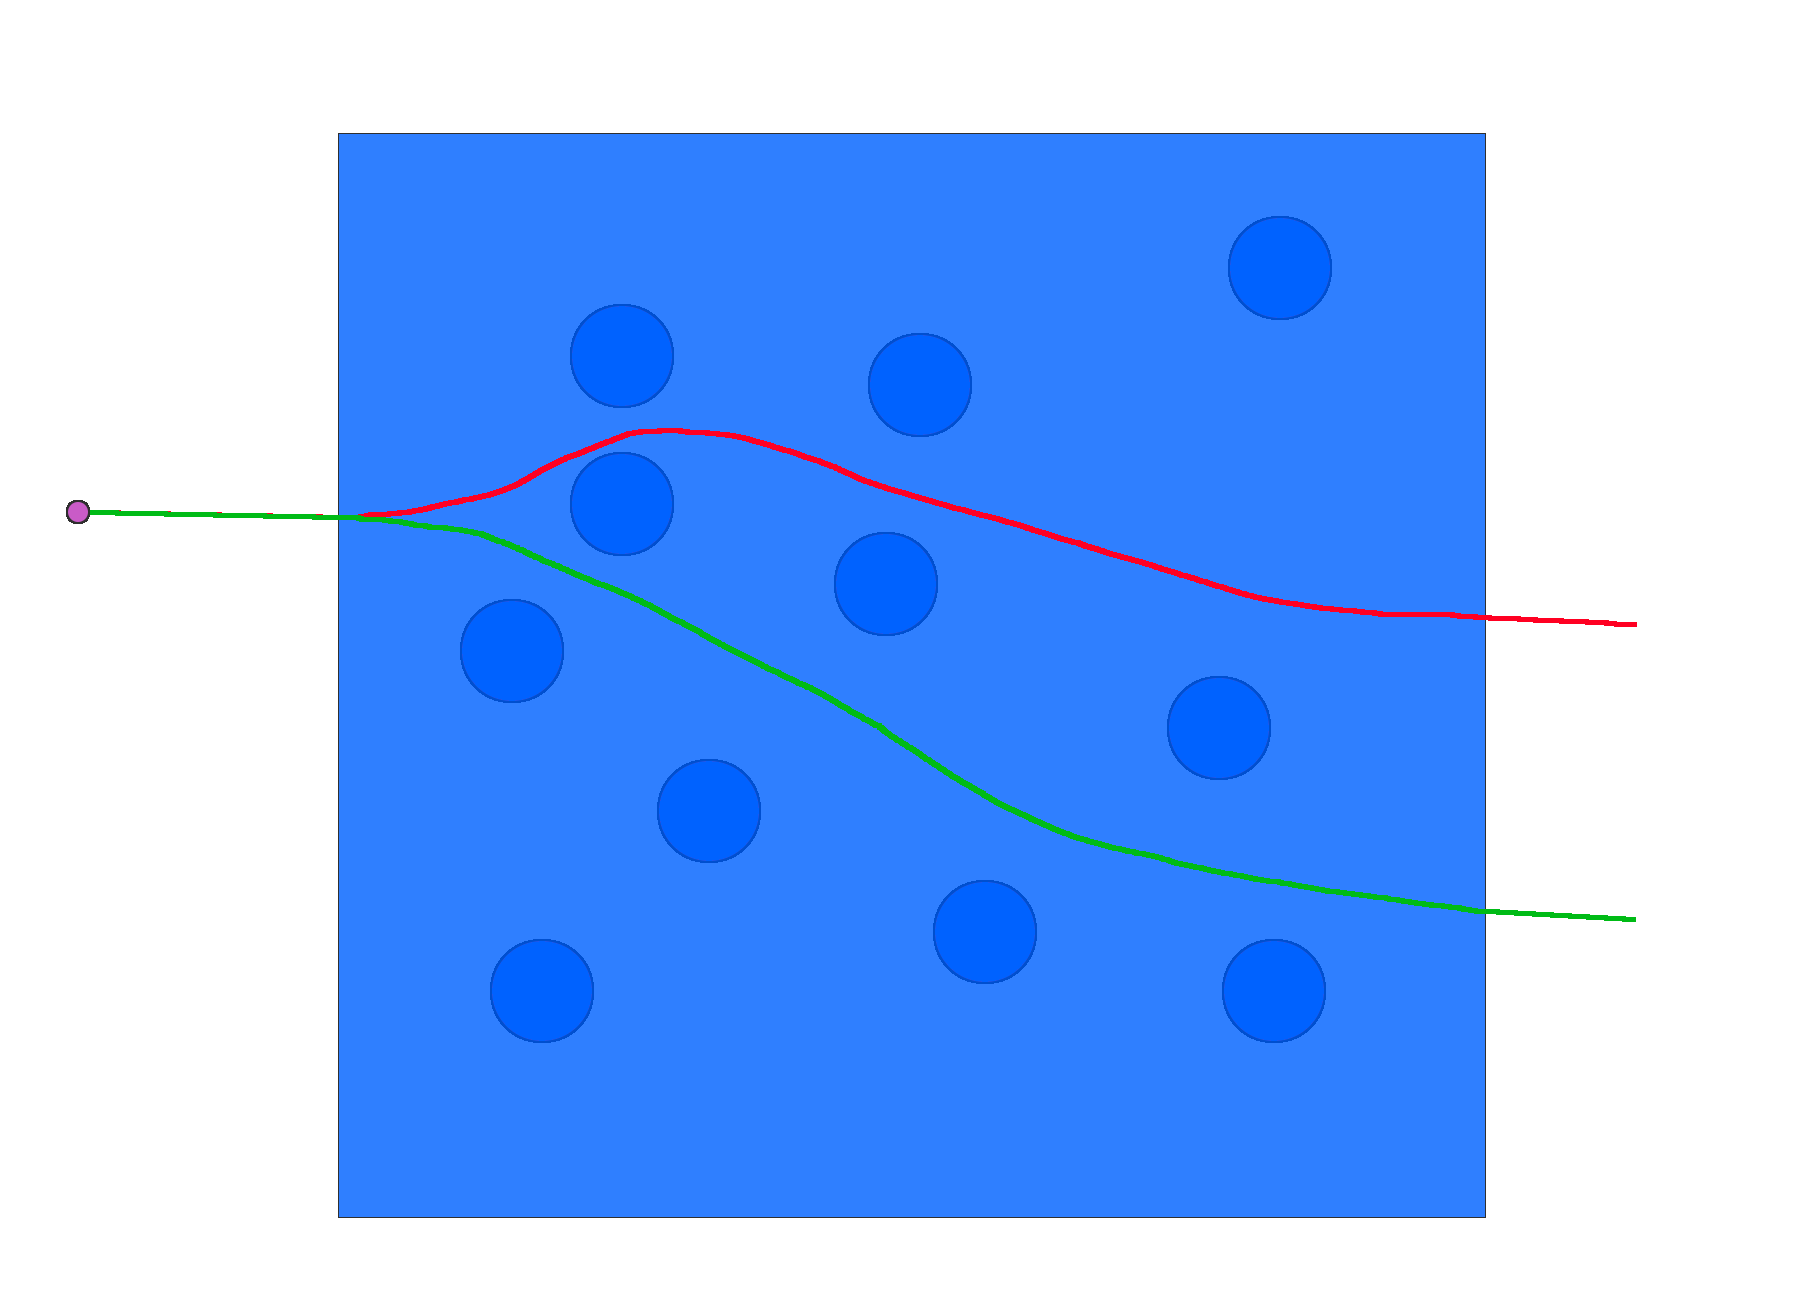
\includegraphics[width=0.75\textwidth]{Figures/lateral_displacement} 
  \caption[Two examples of true paths.]{Two examples of true paths which a particle might take when traversing a medium. Note that both the red and green paths have the same final scattered angle but different transverse positions.}
  \label{fig:lateral_displacement}
\end{figure}

For this reason, transverse corrections have been implemented in  COSY. Due to a lack of experimental data at the time, COSY was compared to G4beamline across several initial momenta and absorber lengths. The result was
\begin{equation}\label{eqn:cosylatdis}
x = x_o + x_D+\text{Gaus}(\theta_\textit{diff} *L/2,\theta_c /(2\sqrt{3})),
\end{equation}
where $x_o$ is the original $x$ position, $x_D = L*P_{x,o}/P_{z,o}$ is the deterministic  gain in $x$, and Gaus($\mu,\sigma$) is a randomly selected number from a Gaussian distribution with mean $\mu$ and standard deviation $\sigma$. The forms of $\mu$ and $\sigma$ were selected based on a combination of the Particle Data Group \cite{PDG} and Fernow and Gallardo  \cite{fernowAndGallardo}. Note that the average $\mu=\theta_\textit{diff}*L/2$ represents the transverse displacement that would have occured if all of the angular scattering had happened at the point $L/2$. $\theta_\textit{diff}=\theta_\textit{final}-\theta_o$ is the amount of deflection which occurred due to scattering and $\theta_c=13.6 \text{ eV}/\beta p \cdot \sqrt{1/X_0}$ is the coefficient from Highland theory \cite{highland}.

The fitting of these parameters is discussed next. As previously mentioned, the data for the fits were generated by G4beamline \cite{g4bl}. Here, a particular example of a simulation of $10^6$ particles passing through 1 cm of liquid hydrogen is shown. The initial beam distribution was a pencil beam of momentum 200 MeV/$c$. A plot of the histogram of $(x,p_x)$ phase space can be seen in Figure~\ref{fig:xpx_phase_space}. It can be seen in Figure~\ref{fig:xpx_phase_space_cut} that the cross section for a given transverse momentum results in a nearly-Gaussian $x$ histogram. It can also be inferred from the figure that the mean and standard deviation of the Gaussian fit vary depending on which $p_x$ is chosen. For example, higher values of $p_x$ appear to have both a larger mean and standard deviation. While this trend is conceptual, it aids in the understanding of the form of Eq. \eqref{eqn:cosylatdis}.

The phase space portrait in Figure~\ref{fig:phase_space_portrait} shows that the distribution is only locally Gaussian. However, fitting in the range of $p=100\text{--}400$ MeV/$c$, $L=1\text{--}100$ mm has shown that this is a good approximation for the majority of particles (see Section~\ref{sec:benchmark}).

An example of the success of this implementation can be seen in Figure~\ref{fig:xpx_phase_space_implemented}, where $10^6$ muons of momentum 250 MeV/$c$ were simulated through 100 mm of liquid hydrogen. The simulation was carried out in both COSY and ICOOL \cite{icool} with good agreement.

\begin{figure}[H]
  \centering
    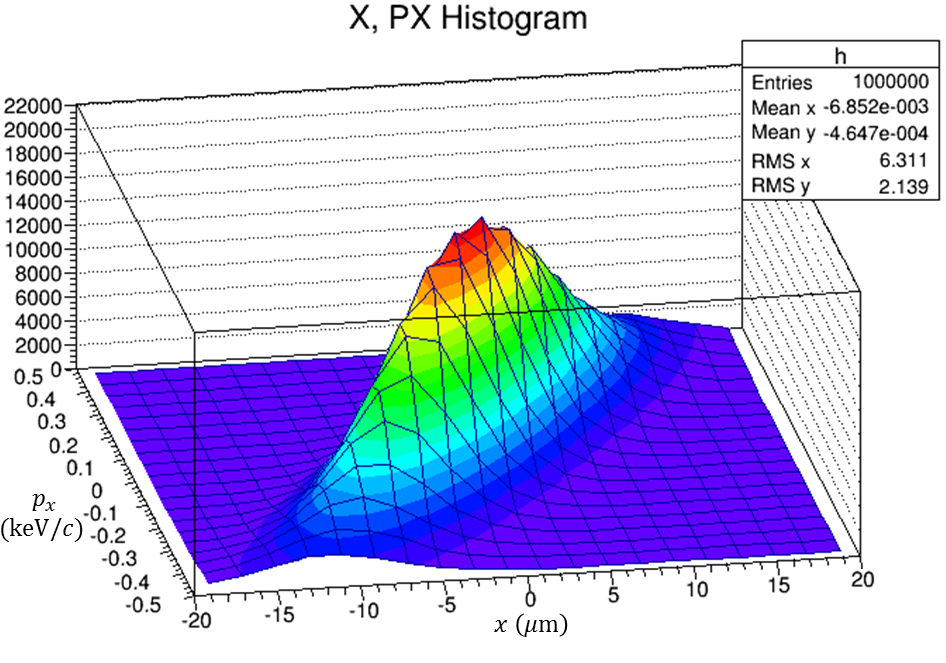
\includegraphics[width=0.7\textwidth]{Figures/xpx_phase_space} 
  \caption[2D histogram of $(x,p_x)$ phase space.]{2D histogram of $(x,p_x)$ phase space for $10^6$ muons of momentum 200 MeV/$c$ passing through 1 cm of liquid hydrogen.}
  \label{fig:xpx_phase_space}
\end{figure}

\begin{figure}[H]
  \centering
    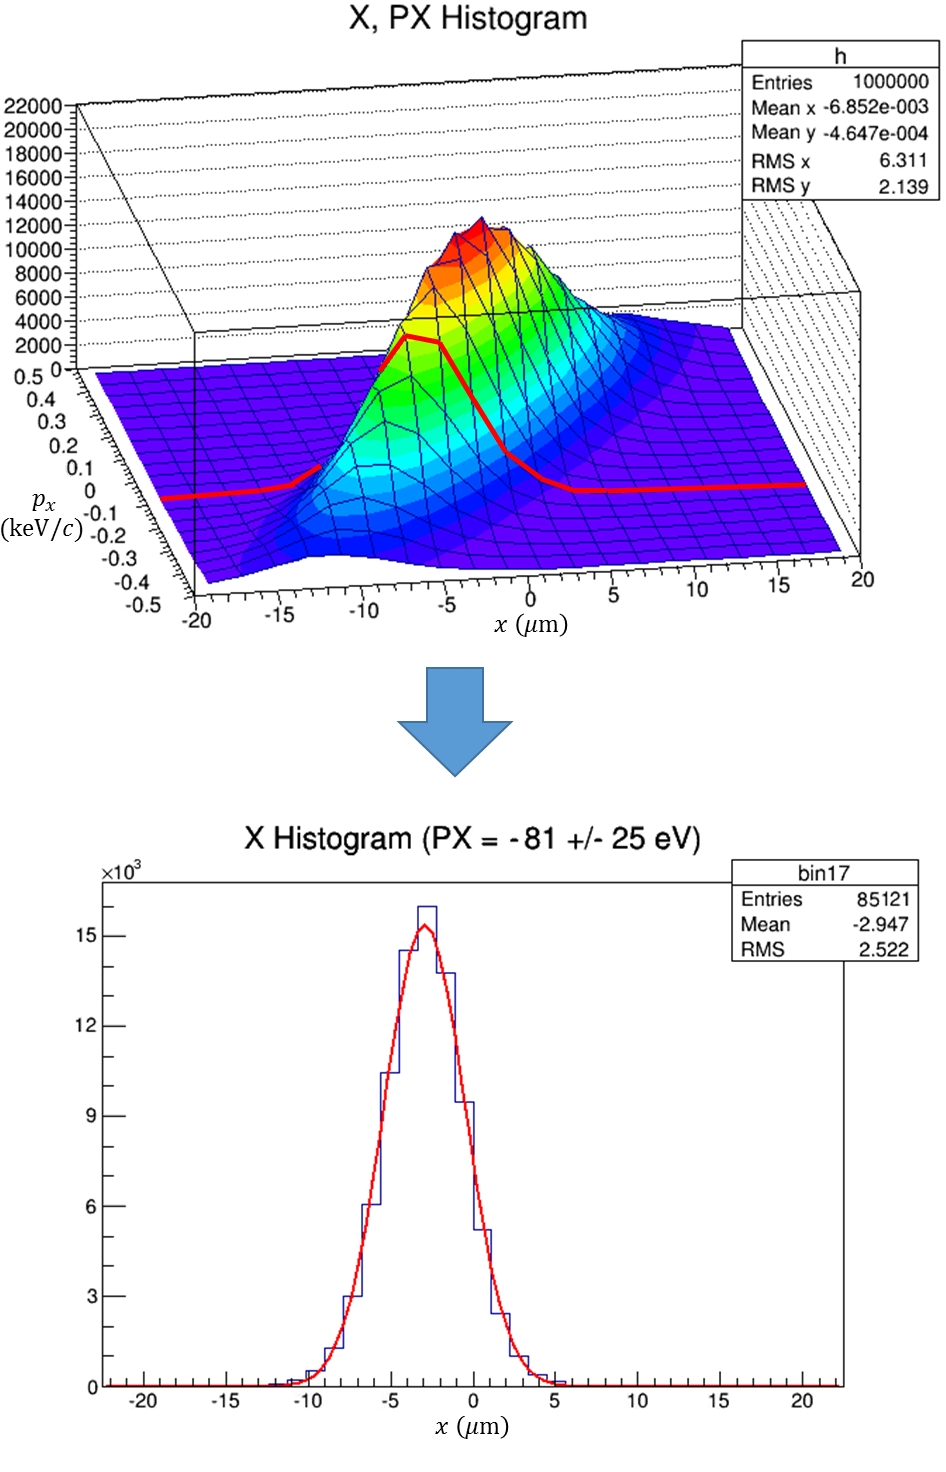
\includegraphics[width=0.7\textwidth]{Figures/xpx_phase_space_cut} 
  \caption[Cross section of Figure~\ref{fig:xpx_phase_space} at $p_x=0.08$ keV/$c$.]{Cross section of Figure~\ref{fig:xpx_phase_space} at $p_x=(-0.081 \pm 0.025)$ keV/$c$. The resulting $x$ histogram is fit (in red) with a Gaussian.}
  \label{fig:xpx_phase_space_cut}
\end{figure}

\begin{figure}[H]
  \centering
    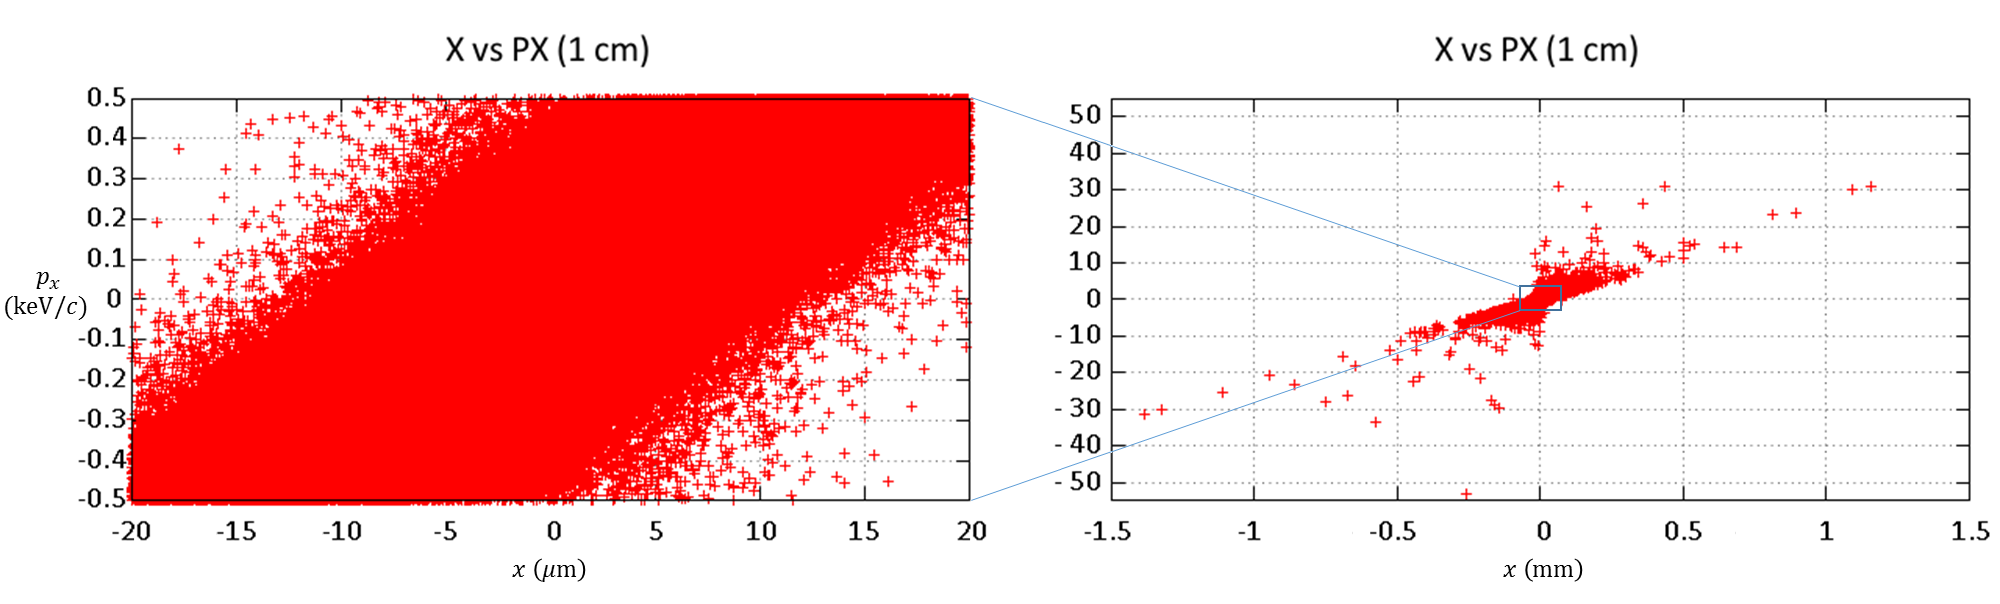
\includegraphics[width=\textwidth]{Figures/phase_space_portrait} 
  \caption[Phase space portrait of Figure~\ref{fig:xpx_phase_space}.]{Phase space portrait of Figure~\ref{fig:xpx_phase_space}. The bulk in Figure~\ref{fig:xpx_phase_space} (left) is approximately Gaussian. The extremities in Figure~\ref{fig:xpx_phase_space} (right) are not approximately Gaussian.}
  \label{fig:phase_space_portrait}
\end{figure}

\begin{figure}[H]
  \centering
    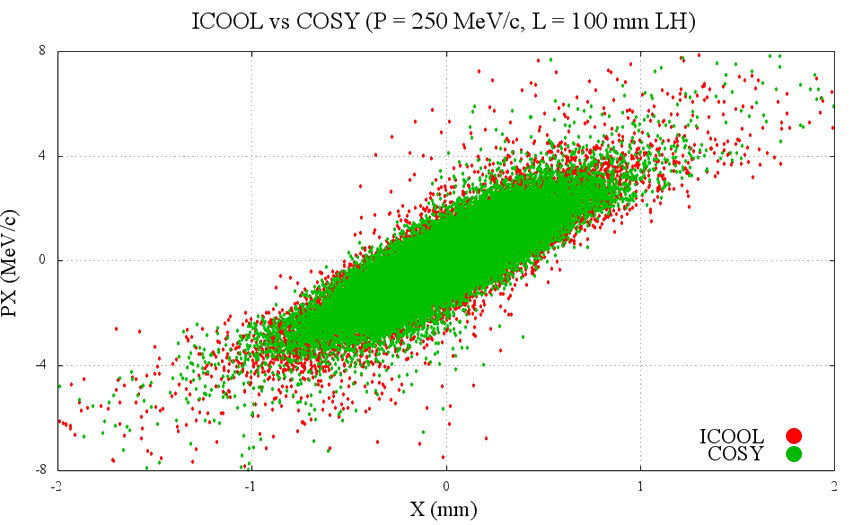
\includegraphics[width=0.7\textwidth]{Figures/xpx_phase_space_implemented} 
  \caption{Sample simulation results for the implementation of the transverse coordinate correction algorithm.}
  \label{fig:xpx_phase_space_implemented}
\end{figure}
%
%-------------------------------------------------------------------------------
%
\Section{Temporal Displacement in COSY Infinity}\label{sec:COSYTemporalDisplacement}\par
The time-of-flight (ToF) is the amount of time it takes for a particle to traverse an absorber. The deterministic ToF is the average time it takes for a particle to traverse an absober and is correlated to the average energy loss. For the ToF in COSY, both the deterministic and stochastic processes are handled in the same routine. To first order, the particle decelerates at some  average rate through an absorber of length $L$. If $a$ is the constant acceleration then 
\begin{align*}
v_f=v_o+a\Delta t,
\end{align*}
or 
\begin{align*}
a=\frac{v_f-v_o}{\Delta t}.
\end{align*}
At the same time, $v_f ^2 = v_o ^2 + 2 a L$, and so
\begin{align*}
 a=\frac{v_f ^2 - v_o ^2}{2L}.
\end{align*}
Then $\Delta t$ becomes
\begin{align*}
\Delta t &= \frac{(v_f-v_o)2L}{v_f^2-v_o^2}=\frac{2L}{v_f+v_o}.
\end{align*}
Given $\beta=pc/E$ and $v=\beta c$, then
\begin{equation}\label{eqn:cosyDeltaT}
%\Delta t=\frac{2L}{\frac{p_f c}{E_f}+\frac{p_o c}{E_o}}.
\Delta t=2L/\left(\frac{p_f c}{E_f}+\frac{p_o c}{E_o}\right).
\end{equation}

However, COSY does not have a time variable, but rather a variable $\ell$ that is described as the time-of-flight in units of length. In COSY \cite{cosy}, this is defined as
\begin{align*}
\ell=\frac{-(t-t_0)v_0\gamma}{1+\gamma},
\end{align*}
where the subscript $0$ signifies the reference particle. Let the time before a step be denoted $t_1$ and the time after a step denoted $t_2$. Then to find $\ell_2$ given $\ell_1$ and $\Delta t$ from Eq. \eqref{eqn:cosyDeltaT}, observe that
\begin{align} \label{eqn:cosyell12}
\begin{split}
\ell_1=\frac{(t_{01}-t_1)v_{01}\gamma_1}{1+\gamma_1} = (t_{01}-t_1)A_1\\
\ell_2=\frac{(t_{02}-t_2)v_{02}\gamma_2}{1+\gamma_2} = (t_{02}-t_2)A_2,
\end{split}
\end{align}
where 
\begin{equation}\label{eqn:cosyAn}
A_n \equiv v_{0n}\gamma_n / (1+\gamma_n) \qquad \text{for }n=1,2
\end{equation}
and the subscript $0$ again denotes the reference particle.
Then
\begin{align*}
\ell_2 - \ell_1 &=\left(t_{02}-t_2\right)A_2-(t_{01}-t_1)A_1\\
&=\left([(t_{02}-t_{01})+t_{01}]-[(t_2-t_1)+t_1]\right)A_2-(t_{01}-t_1)A_1\\
&=(\Delta t_0 - \Delta t )A_2 + (t_{01}-t_1)A_2-(t_{01}-t_1)A_2\\
&=(\Delta t_0 - \Delta t )A_2 + (t_{01}-t_1)(A_2-A_1).
\end{align*}
Eq. \eqref{eqn:cosyell12} says that $t_{01}-t_1=\ell_1/A_1$. Moving $\ell_1$ to the right hand side,
\begin{align*}
\ell_2 &= (\Delta t_0 - \Delta t)A_2 + \frac{\ell_1}{A_1}(A_2-A_1)+\ell_1\\
&=(\Delta t_0 - \Delta t)A_2 + \ell_1\left(\frac{A_2-A_1}{A_1}+\frac{A_1}{A_1}\right)\\
&=(\Delta t_0 - \Delta t)A_2 + \ell_1\frac{A_2}{A_1}.
\end{align*}
Substituting for $A_n$ via Eq. \eqref{eqn:cosyAn} yields the final result
\begin{equation}\label{eqn:cosyell2}
\ell_2=\frac{(\Delta t_0 - \Delta t) v_{02}\gamma_2}{1+\gamma_2}+\ell_1 \frac{v_{02}\gamma_2 (1+\gamma_1)}{v_{01}\gamma_1 (1+\gamma_2)}.
\end{equation}
Using Eq.~\eqref{eqn:cosyell2}, $\Delta t$ from Eq.~\eqref{eqn:cosyDeltaT} can be directly input into the new COSY variable for time-of-flight in units of length. Figure~\ref{fig:longitudinal_phase_space} shows the simulation results for a beam of $10^6$ muons of momentum 172 MeV/$c$ passing through 109 mm of liquid hydrogen, which were the parameters of the MuScat experiment \cite{muscat}. The COSY results are shown alongside those from ICOOL \cite{icool}. Note that the agreement is quite good. ICOOL displays a thicker bulk at around 0.430 ns, but it is approximately 1 ps in width---about 0.2\% of the average time-of-flight.

\begin{figure}[H]
  \centering
    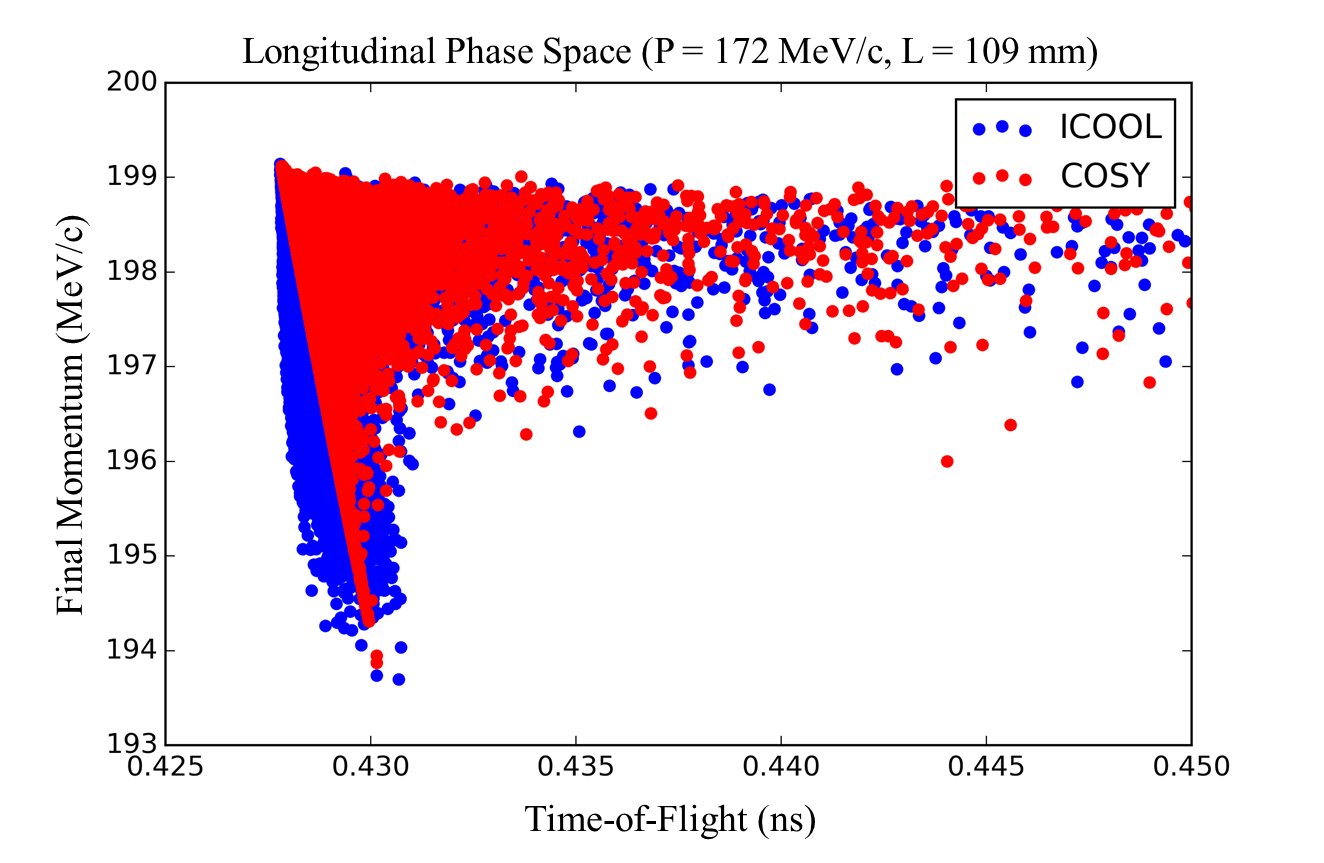
\includegraphics[width=0.7\textwidth]{Figures/longitudinal_phase_space} 
  \caption{Sample simulation results for the implementation of the temporal displacement algorithm discussed in this section.}
  \label{fig:longitudinal_phase_space}
\end{figure}

In conclusion, the two primary stochastic effects, energy straggling and multiple scattering, were discussed at length, resulting in Eqs.~\eqref{eqn:landau} and~\eqref{eqn:MottCrossSection}. The secondary stochastic effects were temporal and transverse displacement, which correspond respectively to energy straggling and multiple scattering. These secondary effects were also elaborated upon, resulting in Eqs.~\eqref{eqn:cosyell2} and~\eqref{eqn:cosylatdis}. The success of these theoretical equations will be discussed in the next section.

\Chapter{Software Implementation}\label{chp:code_implementation}
This chapter discusses in detail the organization and internal structure of the code, which is the implementation of the novel algorithms discussed in Chapter \ref{chp:cosy}. For reference, a reproduction of the code itself may be found in Appendix~\ref{apx:code}. First, the user input is discussed. Next, the \textit{cosy.fox} level of the code is examined. Finally, the structure of the FORTRAN code is briefly considered. Figure~\ref{fig:cosy_flowchart} is referenced during these discussions.

In addition to the user's input file, COSY also uses a \textit{cosy.fox} file. This file contains a plethora of global variables, functions, and routines which the user can access. However, \textit{cosy.fox} can also be used to hide most of the complicated machinery from the user. For example, for this study the routines in \textit{cosy.fox} transform the COSY coordinates $(x, a, y, b, \ell, d)$ into absolute coordinates $(x, p_x, y, p_y, t, E)$\footnote{Recall from Eq. \eqref{eqn:phaseSpaceVector} that $x$ and $y$ are the transverse coordinates; $a=p_x/p_0$; $b=p_y/p_0$; $\ell=-(t-t_0)v_0\gamma/(1+\gamma)$; $\delta=(K-K_0)/K_0$; $E$ is the total energy; $K$ is the kinetic energy; and the subscript $0$ denotes the coordinate of the reference particle.}, and then relays the information to the FORTRAN code. Both the user file and the \textit{cosy.fox} file are written in COSYScript, the programming language of COSY. 

\begin{figure}[!htb]
  \centering
    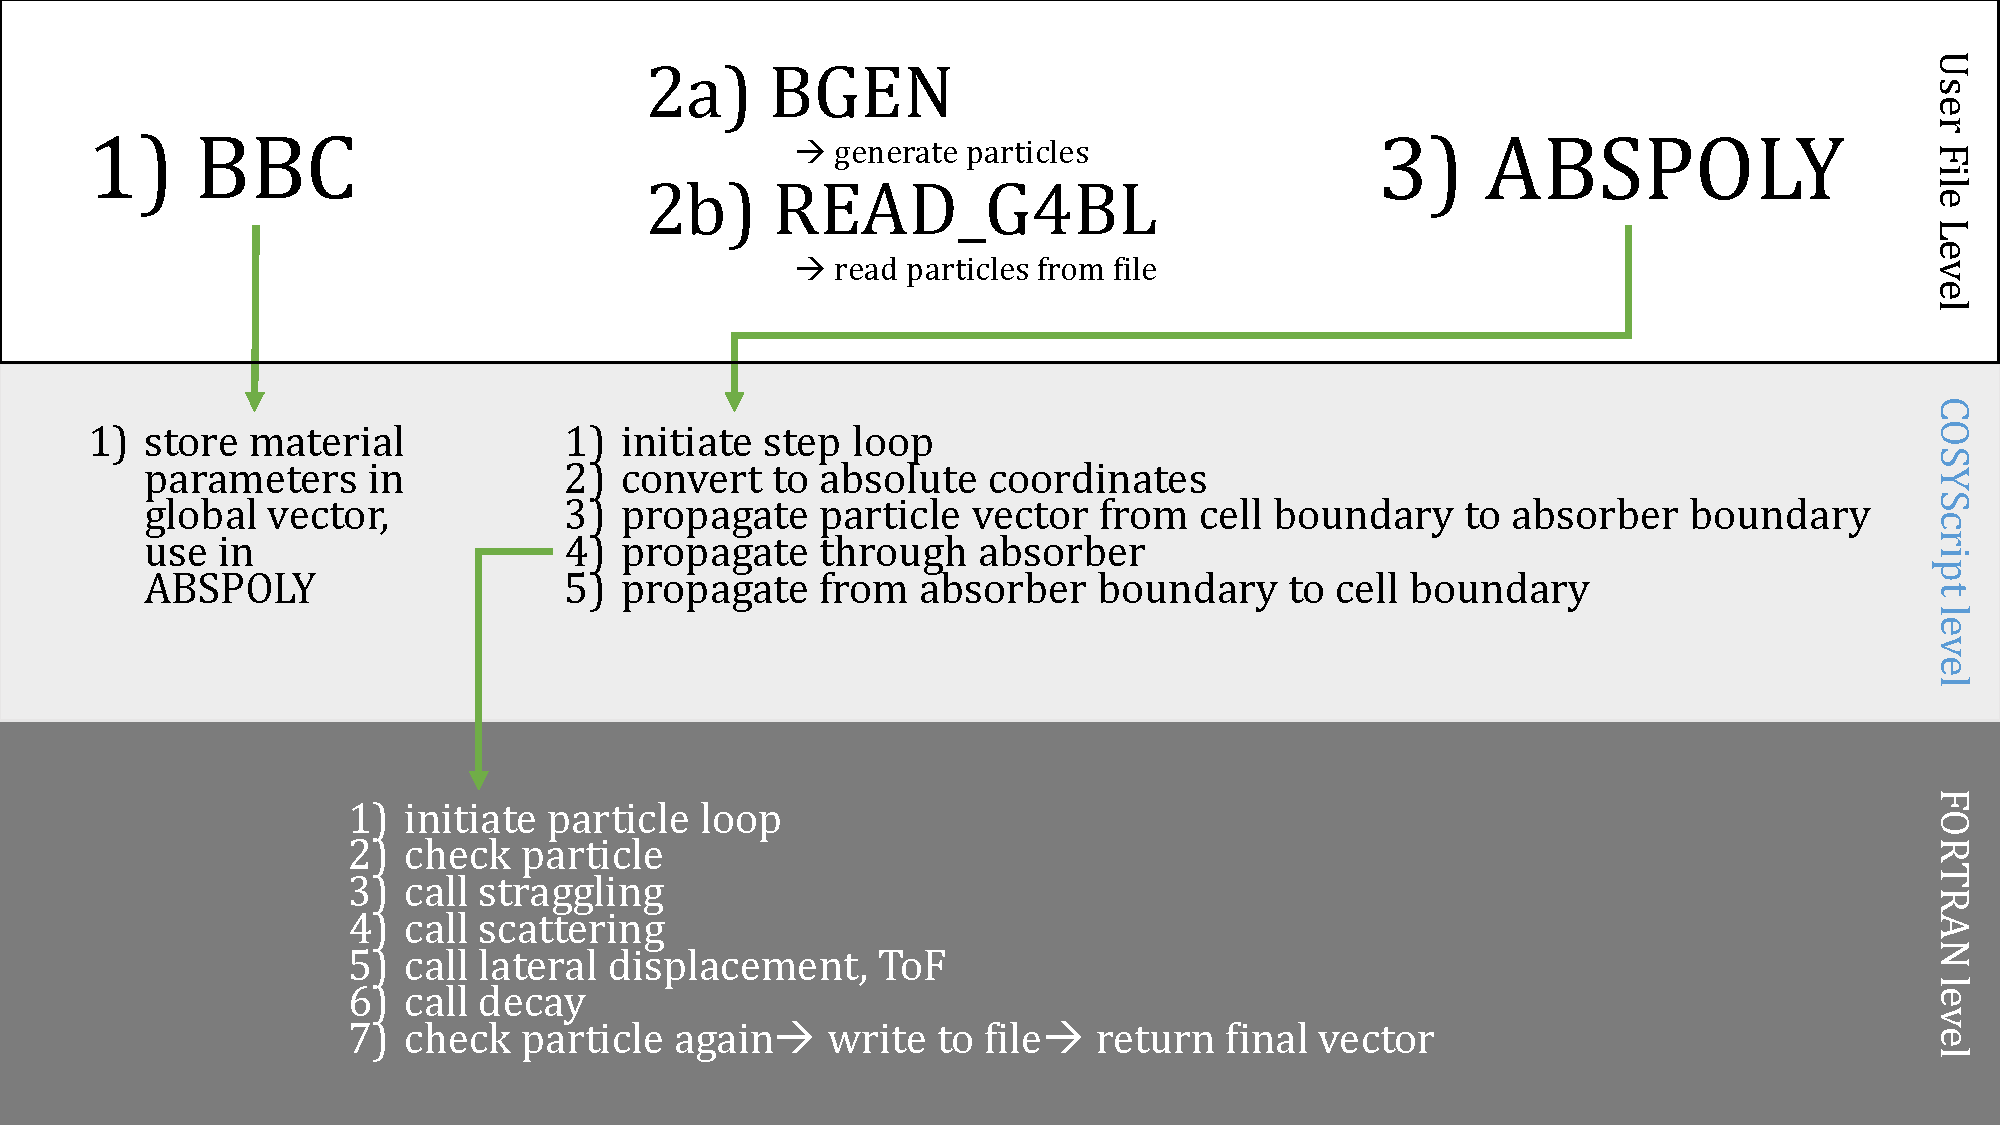
\includegraphics[width=\textwidth]{Figures/cosy_flowchart} 
  \caption{A flowchart for the structure of the new COSY routines implemented in this work.}
  \label{fig:cosy_flowchart}
\end{figure}

\Section{User Input}\label{ssc:user_input}

As with the deterministic absorber routine previously present in COSY, \texttt{WA}, the user must first call the procedure\\
\texttt{BBC} <$Z$> <$A$> <$\rho$> <$I$> <$\delta$> <$C$> \texttt{;} \\
This stores the material parameters in a global array. The arguments are the nuclear charge $Z$, the atomic mass $A$, the density of the material $\rho$, the ionization energy $I$, the density correction $\delta$, and the shell correction $C$. Next, the user must either generate a distribution of particles or read a distribution of particles from a file. Using \\
\texttt{BGEN} <$n$> <$V$> <$\mu_x$> <$\sigma_x$> <$\mu_{p_x}$> <$\sigma_{p_x}$> <$\mu_y$> <$\sigma_y$> <$\mu_{p_y}$> <$\sigma_{p_y}$> <$\mu_t$> <$\sigma_t$> <$\mu_{p_z}$> <$\sigma_{p_z}$> \texttt{;}\\
the user can generate a Gaussian beam of $n$ particles into a 2D vector $V$. Note that in COSY, a 2D vector is a vector of vectors and is not the same data class as an array. Alternatively, the user may use \\
\verb|READ_G4BL| <\texttt{file}> <$n$> <$V$> \texttt{;}\\
to read a G4Beamline-formatted file of $n$ particles and store it into a 2D vector $V$. Finally, the user can call\\
\texttt{ABSPOLY} <$S_1$> <$S_2$> <$n$> <$L$> <$A$> <$V$> <$X_0$> <$S_n$> <$L_c$> <$O$> \texttt{;}\\
where $S_1$\footnote{For a full description of the entrance and exit polynomials $S_1$ and $S_2$, please see the COSY beam physics manual \cite{cosy}, page 33.} is an $n^{th}$ order polynomial describing the entrance surface, $S_2$ is an $n^{th}$ order polynomial describing the exit surface, $L$ is the on-axis length of the absorber, $A$ is the aperture, $V$ is the 2D input and output particle vector, $X_0$ is the radiation length of the material, $S_n$ is the number of steps inside the absorber, $L_c$ is the length of the absorber cell, and $O$ is the output unit number (e.g. ``12'' to save the results in \texttt{fort.12}). A depiction of the parameters can be found in Figure~\ref{fig:abspoly}.

\begin{figure}[!htb]
  \centering
    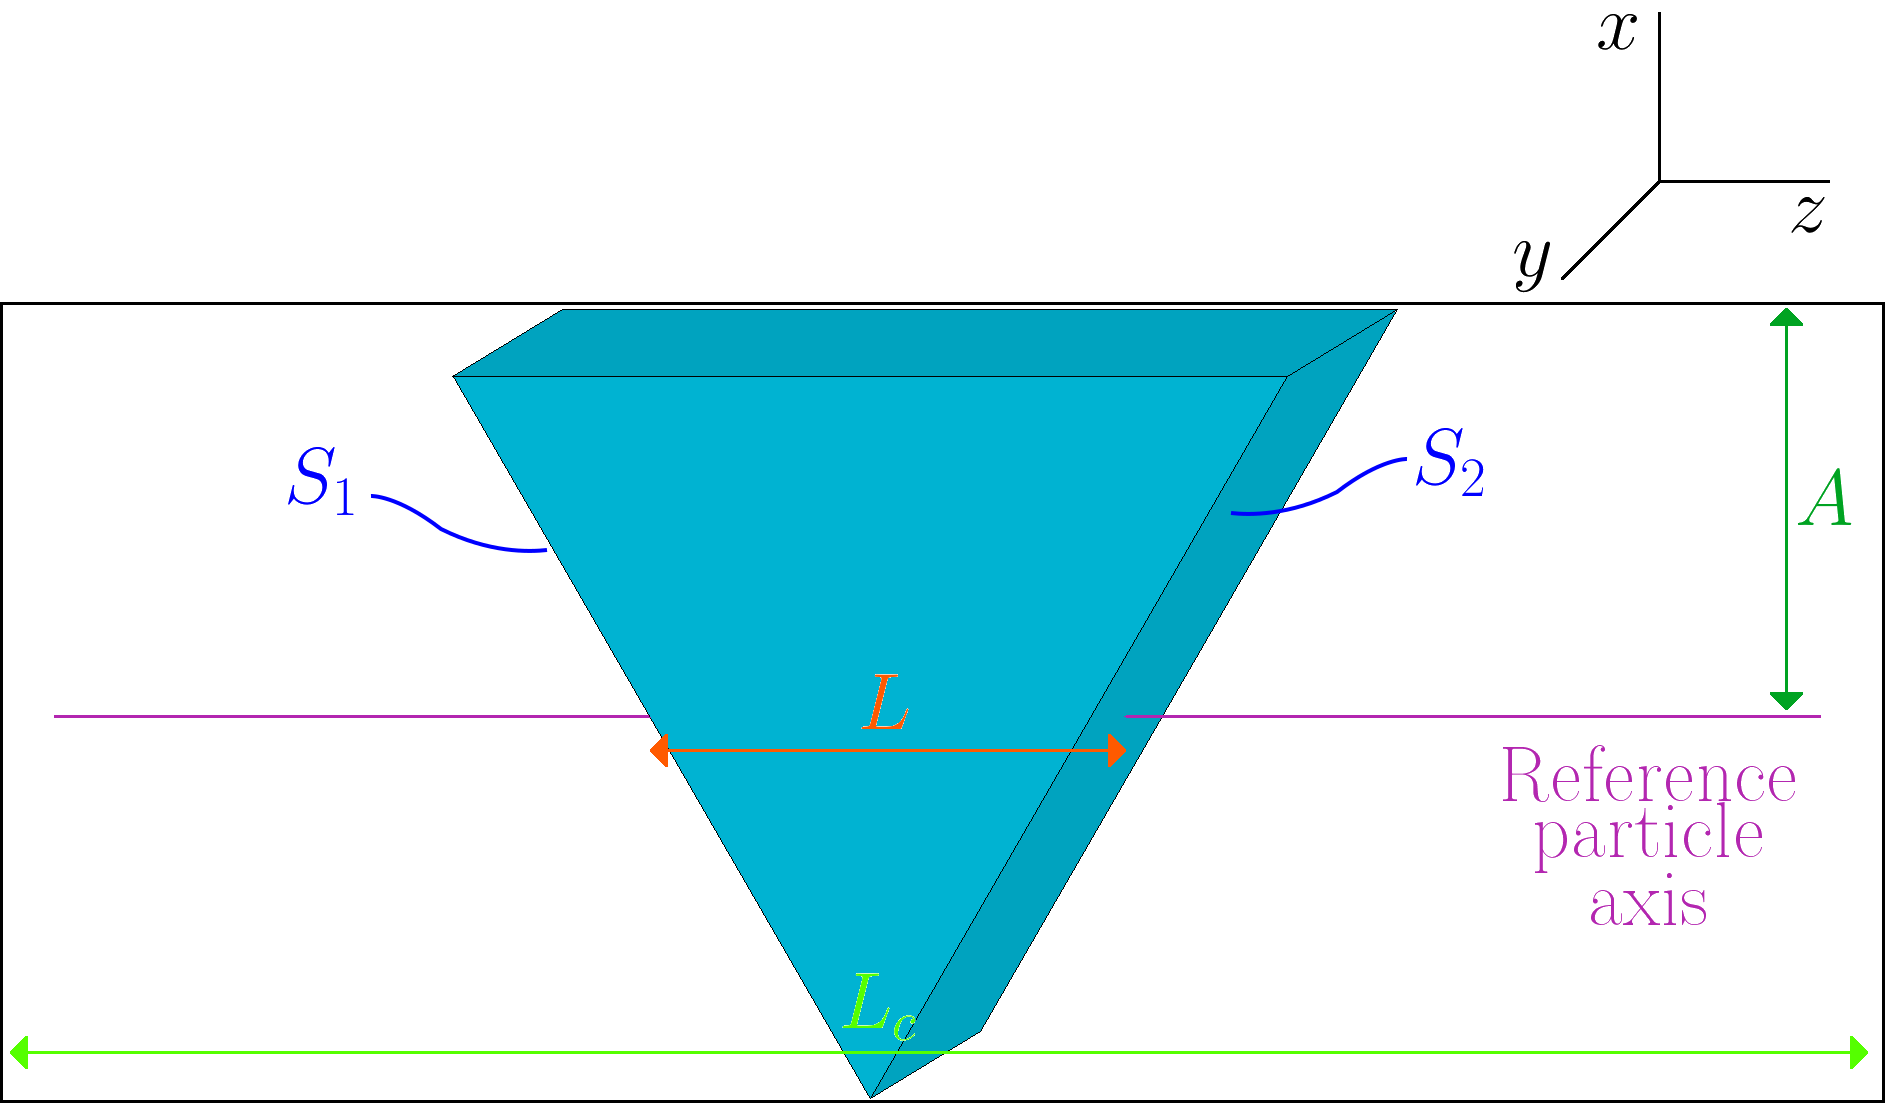
\includegraphics[width=\textwidth]{Figures/abspoly} 
  \caption{Cartoon example of some of the \texttt{ABSPOLY} parameters.}
  \label{fig:abspoly}
\end{figure}

\Section{COSYScript Level}\label{ssc:cosyscript}

As previously mentioned, the \texttt{ABSPOLY} routine is defined in the external file \textit{cosy.fox}. Here, the step loop over $S_n$ is initialized. Next, input 2D vector $V$ is converted from coordinates relative to the reference particle to absolute coordinates. The particle vector is then propagated from the cell boundary (whose width is defined by $L_c$) to the absorber (whose on-axis width is defined by $L$). If $L_c<L$ then no propagation occurs. When the particles are at the absorber boundary, the 2D particle vector $V$ is passed on to the FORTRAN level of the code, where propagation through the absorber takes place. The routine linking the COSYScript and FORTRAN levels is \texttt{STOABS} and is discussed in Section~\ref{ssc:fortran}. After the 2D particle vector $V$ is returned, $V$ is propagated to the end of the cell and returned to the user.

\Section{FORTRAN Level}\label{ssc:fortran}

Except for the propagation of particles through the absorber, the processes found in Section~\ref{ssc:cosyscript} are much faster in COSYScript than in FORTRAN. This is because processes like coordinate conversion, propagation through a vacuum, etc. are deterministic and can therefore be handled by transfer maps.

The routine\\
\texttt{STOABS} <$V$> <$m$> <$L$> <$MP$> <$X_0$> <$O$> <$A$> <$n$> \texttt{;} \\
takes input parameters from the COSYScript level and returns the input 2D particle vector $V$. Here, $m$ is the particle mass (taken from the reference particle), $L$ is an $n$-dimentionial array containing the path lengths for each particle, $MP$ is an array containing the material parameters (taken from the global array $BETHEBLOCHC$ set up by the routine \texttt{BBC}), $X_0$ is the radiation length of the material, $O$ is the output unit number, $A$ is the aperture, and $n$ is the number of particles.

Once the FORTRAN level has this information, a loop over $n$ particles is started. Each particle is checked at the beginning of each loop for the following flags: particle stopped, particle hit aperture, particle missed absorber, drift. If either the particle was stopped ($E\leq m$) or the particle hit the aperture ($x^2+y^2>=A^2$) then the particle is terminated. If the particle missed the absorber completely then the drift flag is turned on. If the drift flag is on then the particle is simply propagated without the stochastic processes called.

Provided that the particle has not been flagged, the particle is subject to energy straggling and then multiple scattering. After these two routines, the lateral displacement and time-of-flight corrections are called. It should be noted that the order matters for energy straggling and multiple scattering. The order does not matter for lateral displacement and time-of-flight provided that both straggling and scattering have already occurred. Finally, decay can be called. Note that for this work, decay has been turned off completely, and so this step is skipped.

Finally, the particle is checked again. If the output unit number $O$ is not equal to zero then the particles are written to a file. Lastly, the 2D particle vector $V$ is returned to the COSYScript level.

\Section{Summary}

Figure~\ref{fig:cosy_flowchart} displays the conceptual process of operating the implemented routines. First, the user defines the material parameters in \texttt{BBC}, which stores these parameters as global variables in the COSYScript level. Next, the user creates a 2D vector of particles, either by generating a Gaussian beam via \texttt{BGEN} or reading particles from a G4Beamline file via \verb|READ_G4BL|. Finally, the user calls the \texttt{ABSPOLY} routine. \texttt{ABSPOLY} converts the COSY coordinates to and from absolute coordinates and calls the FORTRAN routine to step through the absorber. On the FORTRAN level, each particle is subjected to the energy straggling, multiple scattering, transverse displacement, and time-of-flight algorithms described in Chapter \ref{chp:cosy}. These particles are returned to the user at the end of the propagation.

\Chapter{Results}\label{chp:results}
\par In this chapter, the new COSY routines are benchmarked against both ICOOL and G4beamline for pencil beams. Recall that a pencil beam is a beam with an RMS of zero for all transverse coordinates. Pencil beams are used in order to simulate a plethora of possible paths and energy losses for a particular initial condition. Both validation against past experiments and studies of current muon ionization cooling channel (MICE) are shown. Since both ICOOL and G4beamline have automatic variable stepping, their maximum step sizes are left as default unless explicitly stated otherwise.

\Section{Benchmark Against Other Codes}\label{sec:benchmark}

This section briefly discusses the comparison of the new COSY routines with those of two other codes, ICOOL \cite{icool} and G4beamline \cite{g4bl}. Refer to Figures \ref{fig:100.1}--\ref{fig:400.100} (12 figures, each with three subplots) mentioned here. The benchmarking was done over both the typical momentum range of cooling channels (100, 200, 300, and 400 MeV/$c$) and various absorber lengths (1, 10, and 100 mm). These simulations were performed using a pencil beam of $5\times 10^4$ muons with the aforementioned momenta through liquid hydrogen. Note that for the transverse position and transverse momentum histograms, the absolute value of the coordinate is plotted. Therefore, the mean is not zero. For COSY, the step size was the entire absorber length. For G4beamline in the case of a 1 mm absorber, the maximum step size was limited to 0.1 mm. This was done because of the heavy dependence of the transverse position on step size for short absorbers in G4beamline.
\newpage
\begin{figure}[H]
  \centering
    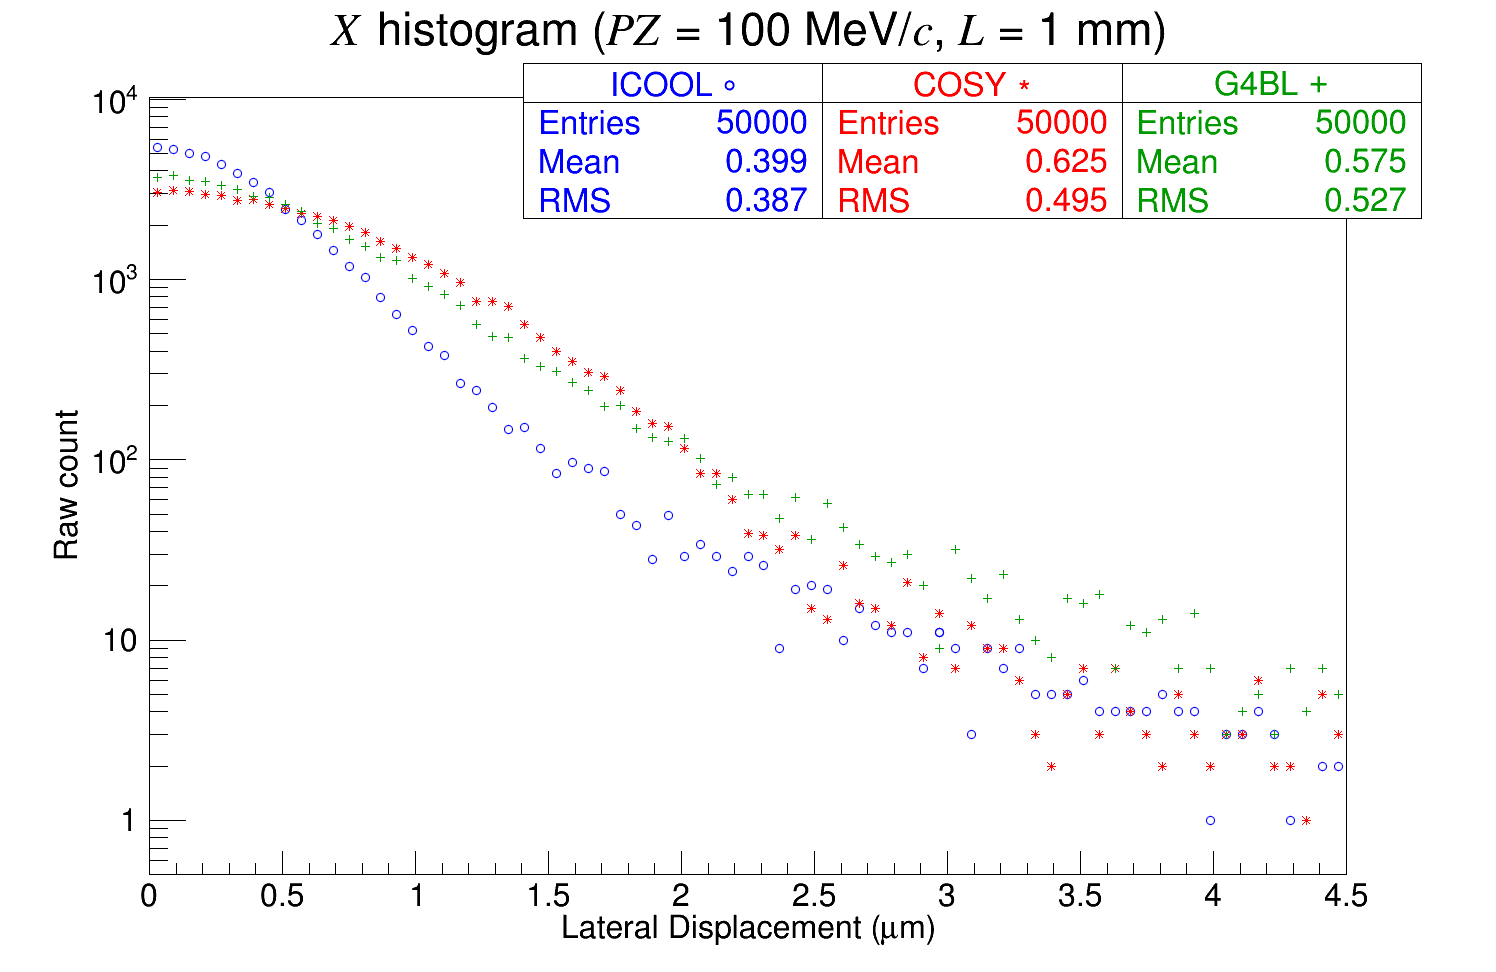
\includegraphics[width=0.7\textwidth]{Benchmarking/LH/X.100.1.png} 
    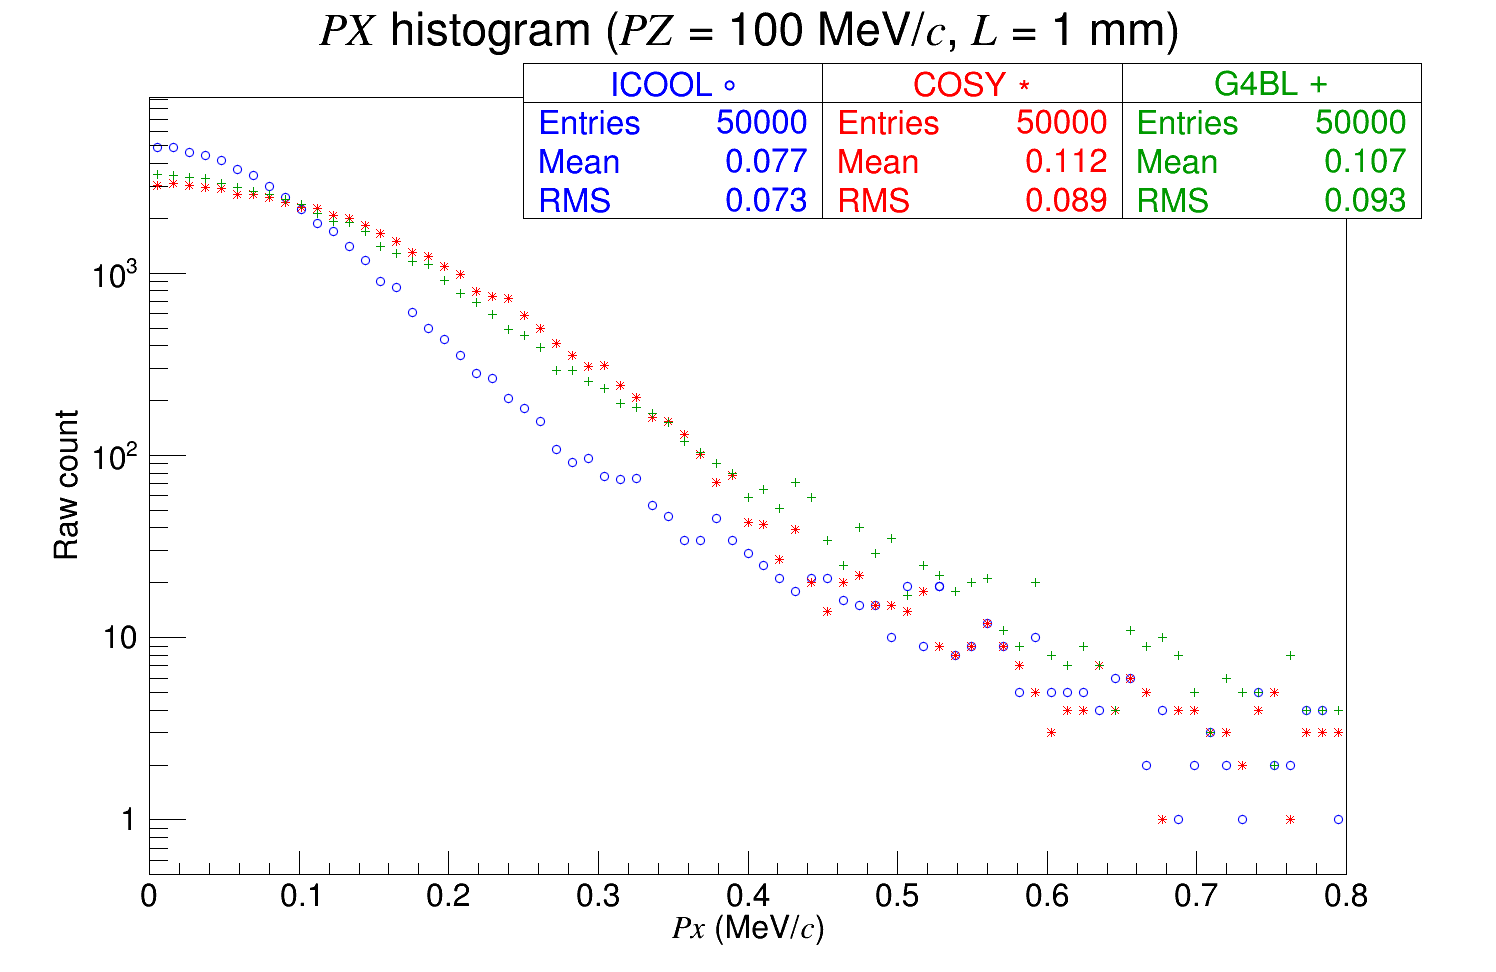
\includegraphics[width=0.7\textwidth]{Benchmarking/LH/PX.100.1.png} 
    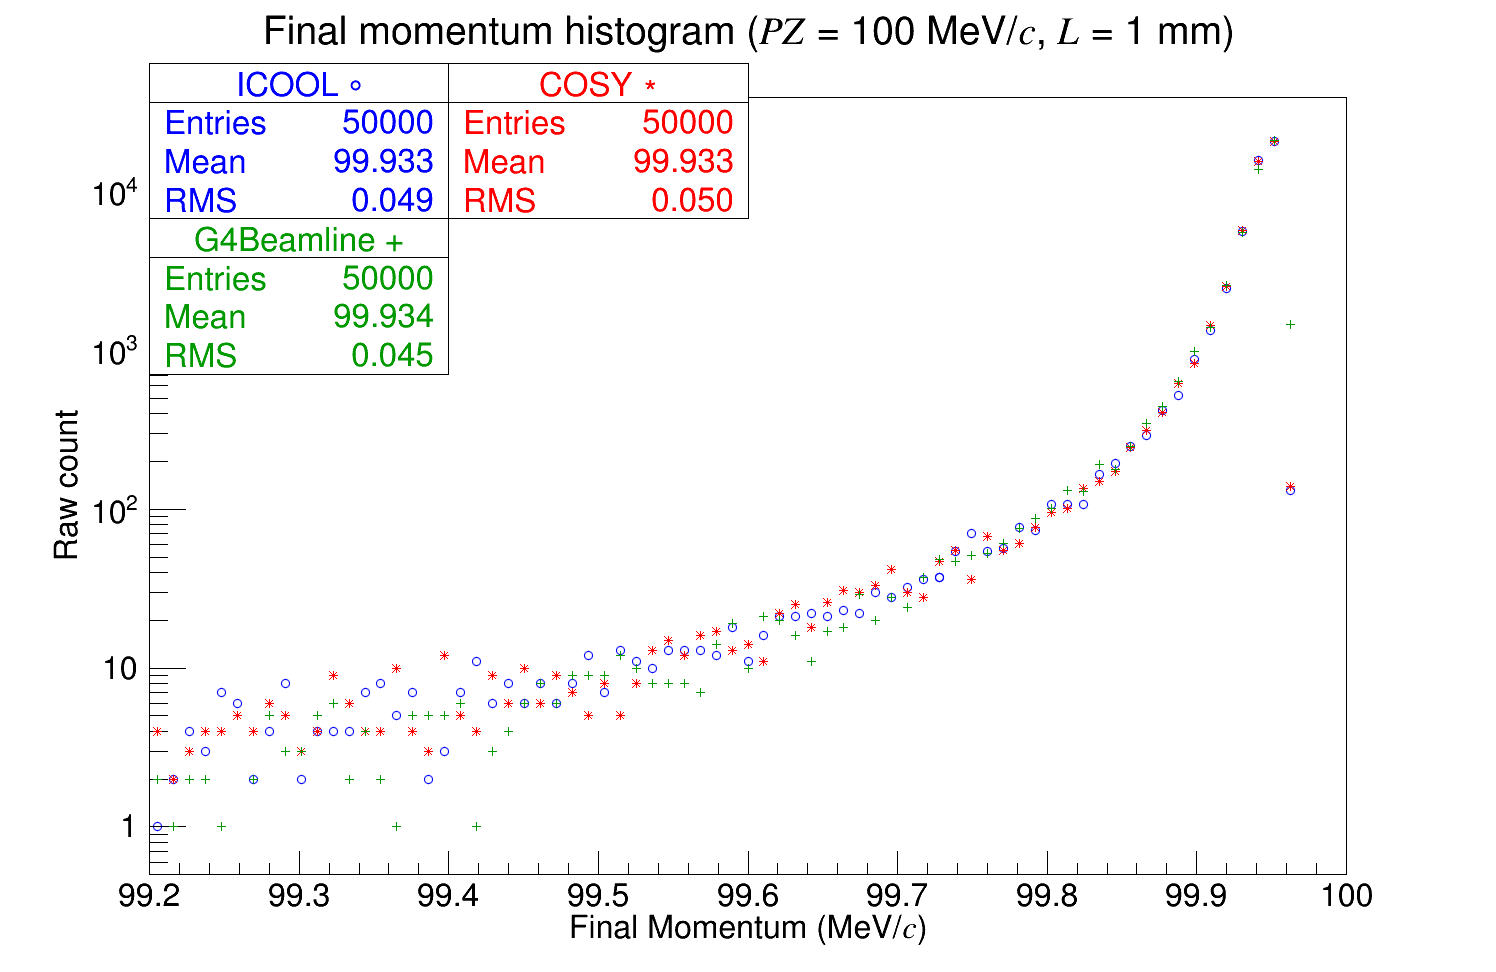
\includegraphics[width=0.7\textwidth]{Benchmarking/LH/strag.100.1.png} 
  \caption[Muons of momentum 100 MeV/$c$ through 1 mm liquid hydrogen.]{Muons of momentum 100 MeV/$c$ through 1 mm liquid hydrogen. For the $x$ and $p_x$ histograms, COSY and G4beamline follow a Gaussian-like peak whereas ICOOL follows a Fano peak.}
  \label{fig:100.1}
\end{figure}

\begin{figure}[H]
  \centering
    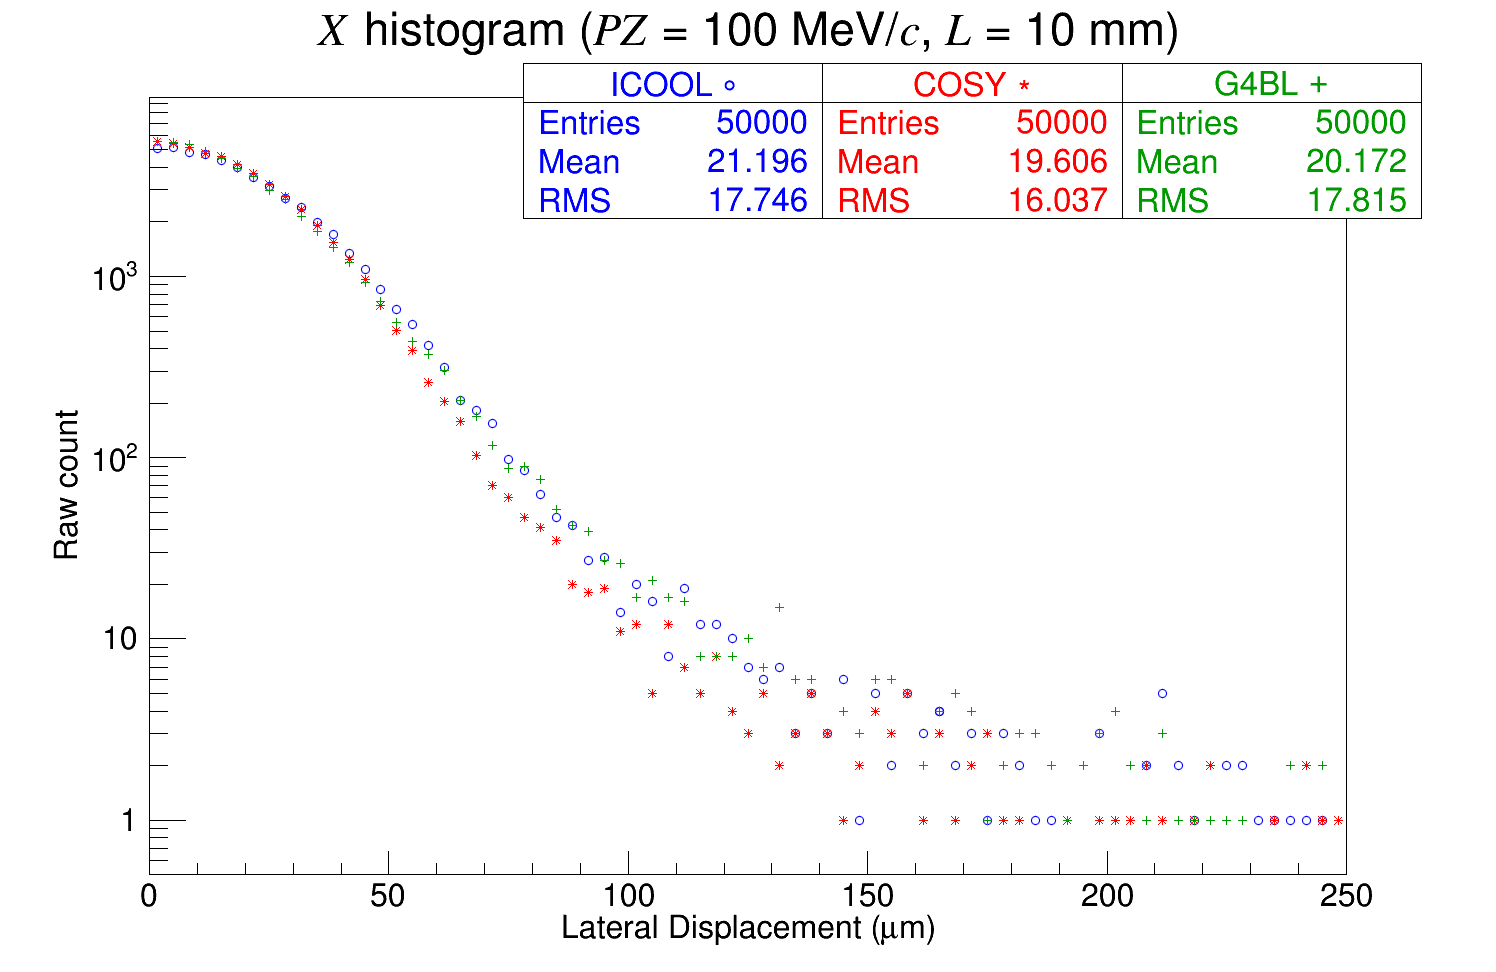
\includegraphics[width=0.7\textwidth]{Benchmarking/LH/X.100.10.png} 
    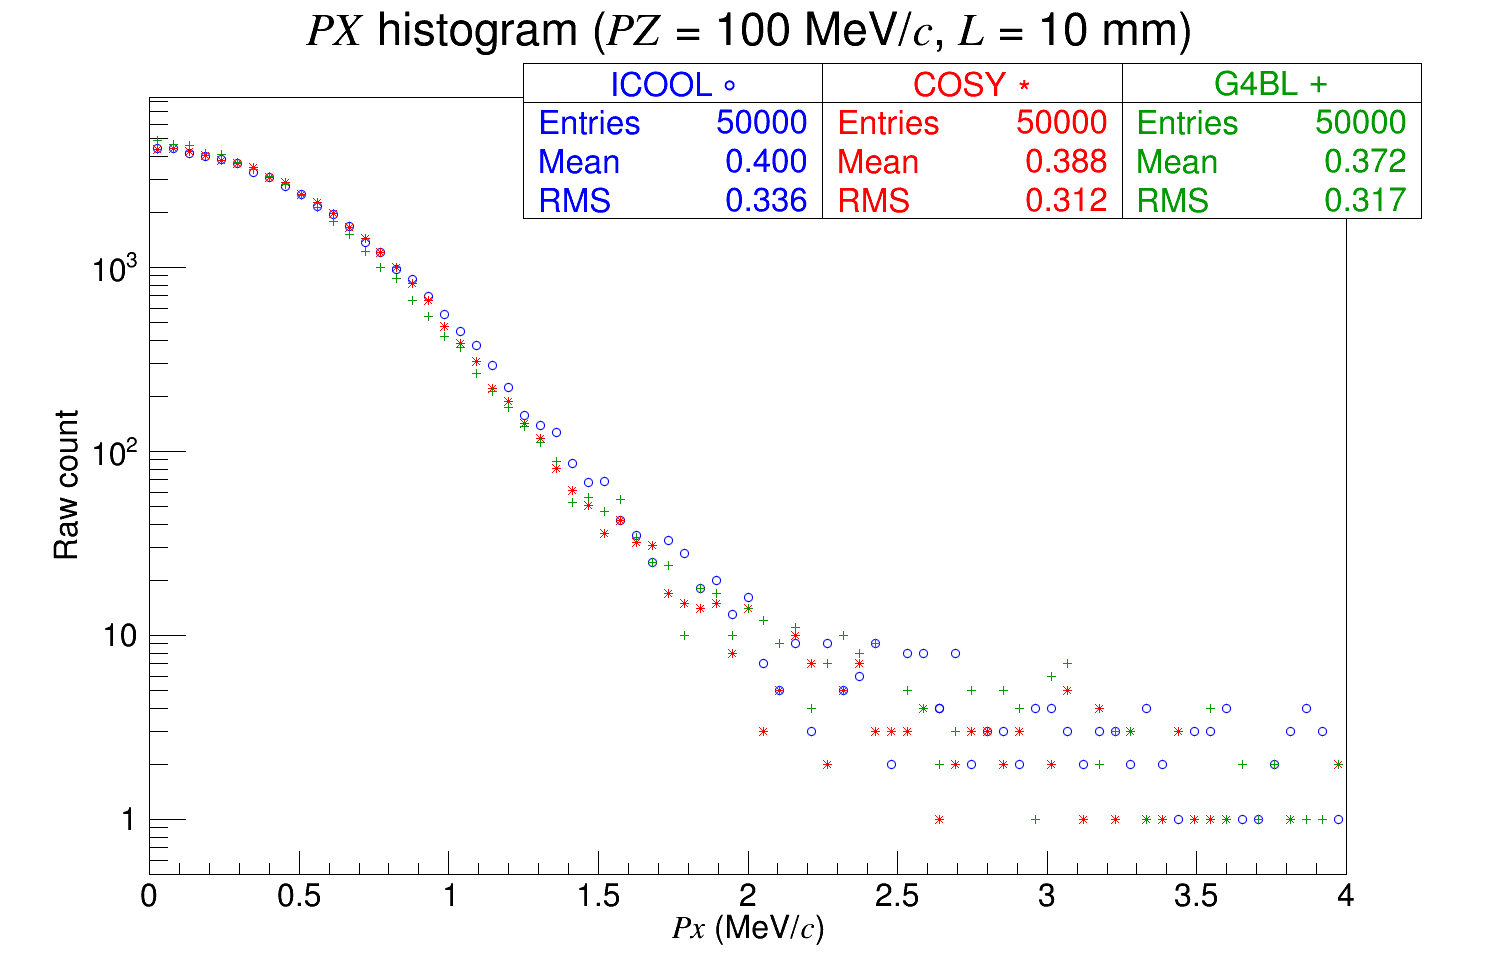
\includegraphics[width=0.7\textwidth]{Benchmarking/LH/PX.100.10.png} 
    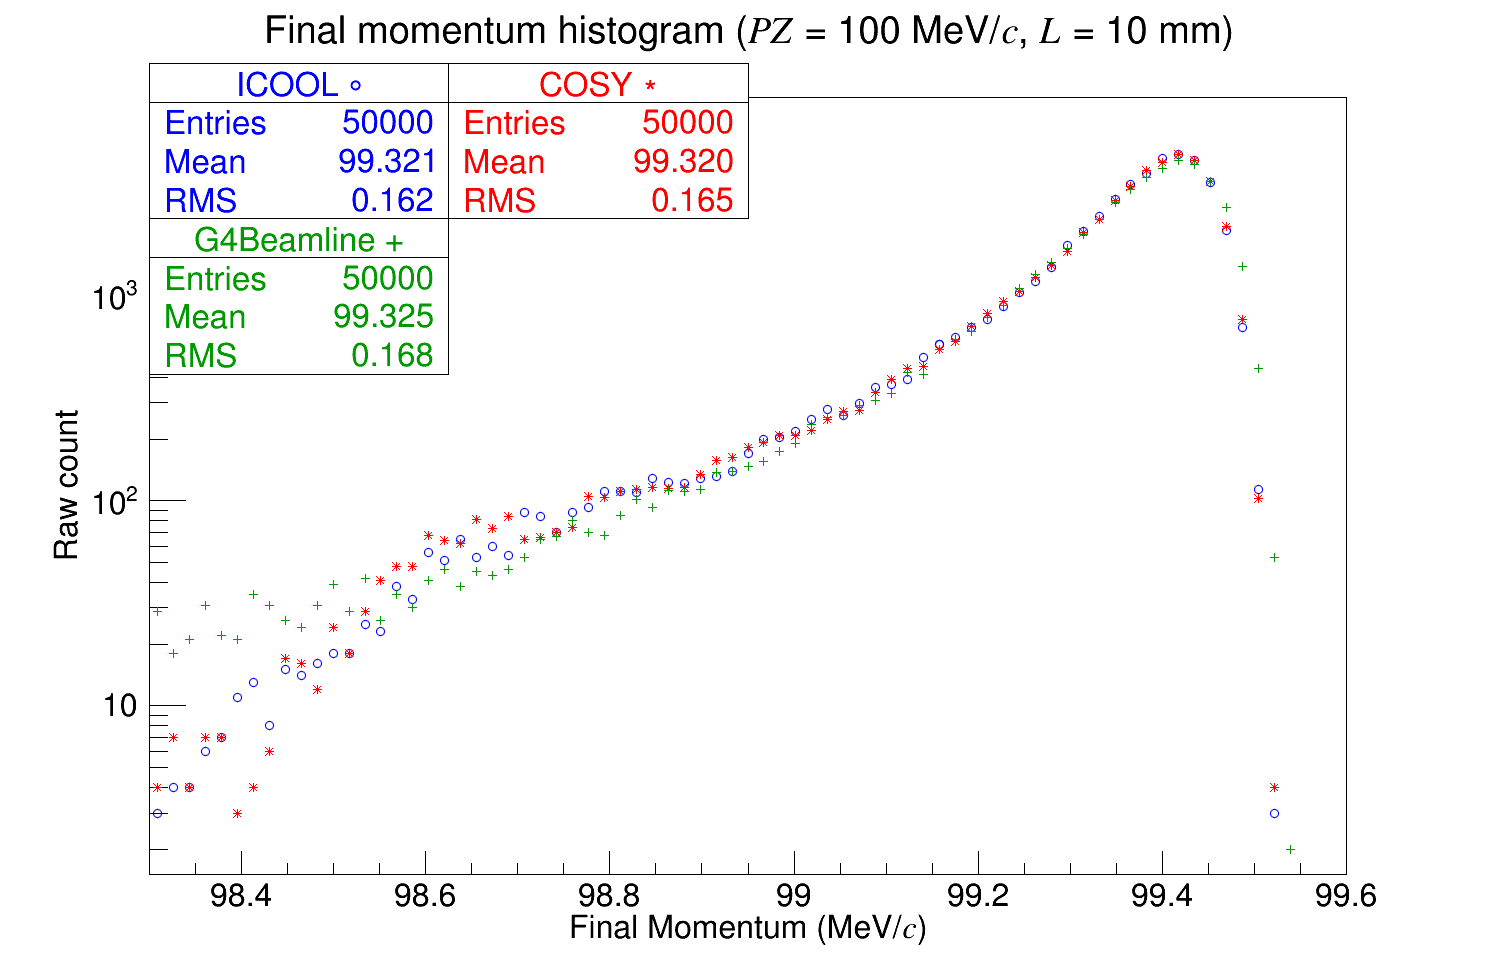
\includegraphics[width=0.7\textwidth]{Benchmarking/LH/strag.100.10.png} 
  \caption{Muons of momentum 100 MeV/$c$ through 10 mm liquid hydrogen.}
  \label{fig:100.10}
\end{figure}

\begin{figure}[H]
  \centering
    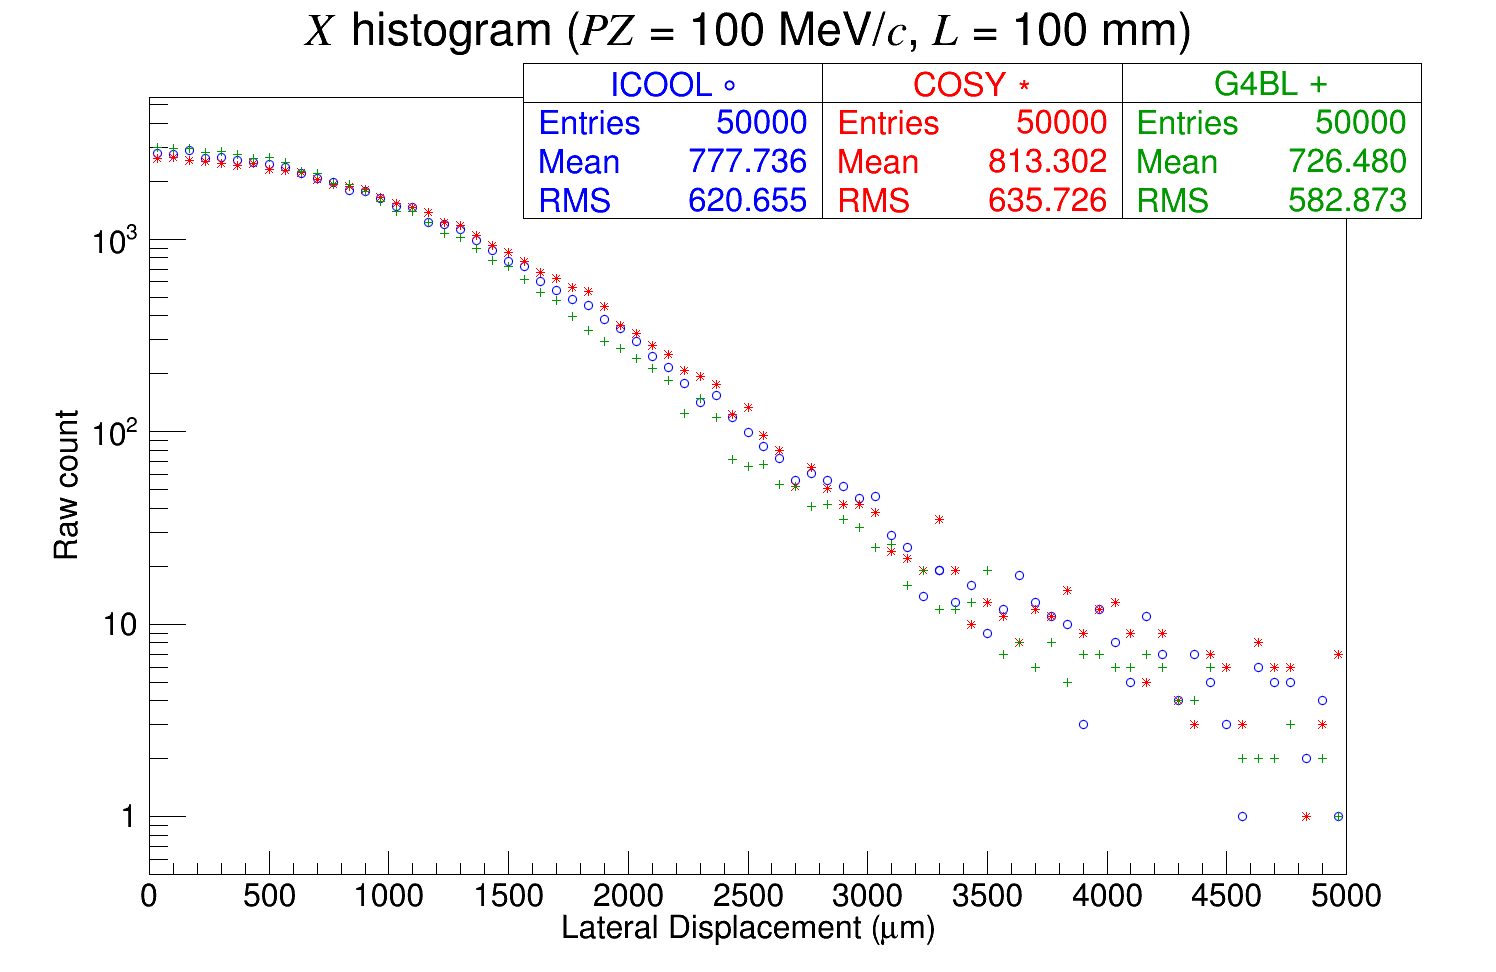
\includegraphics[width=0.7\textwidth]{Benchmarking/LH/X.100.100.png} 
    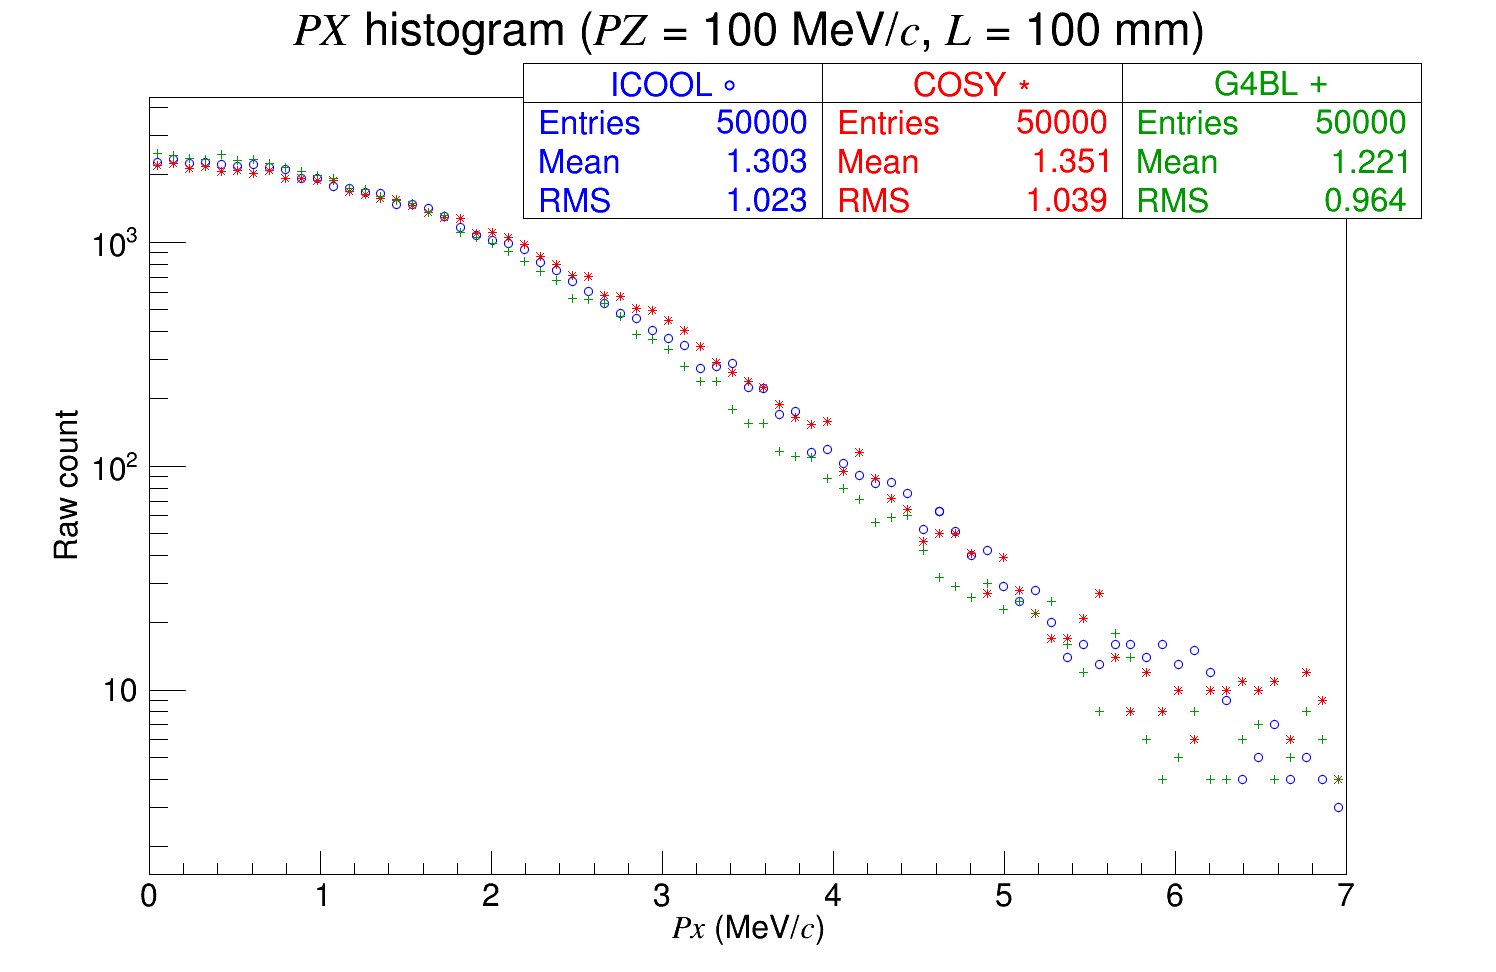
\includegraphics[width=0.7\textwidth]{Benchmarking/LH/PX.100.100.png} 
    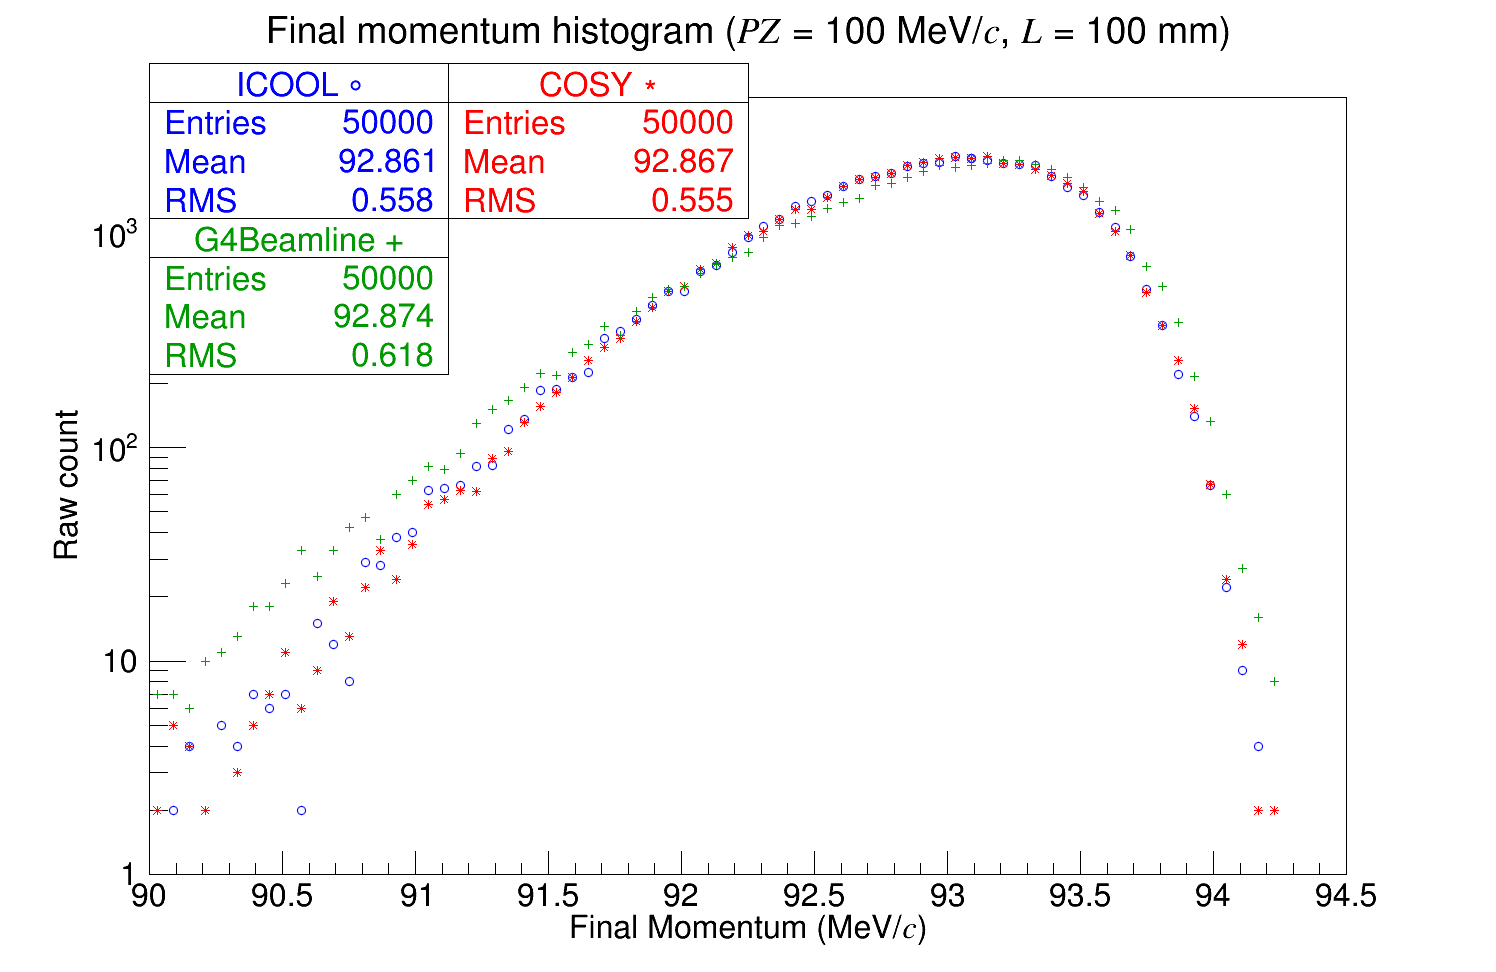
\includegraphics[width=0.7\textwidth]{Benchmarking/LH/strag.100.100.png} 
  \caption{Muons of momentum 100 MeV/$c$ through 100 mm liquid hydrogen.}
  \label{fig:100.100}
\end{figure}

\begin{figure}[H]
  \centering
    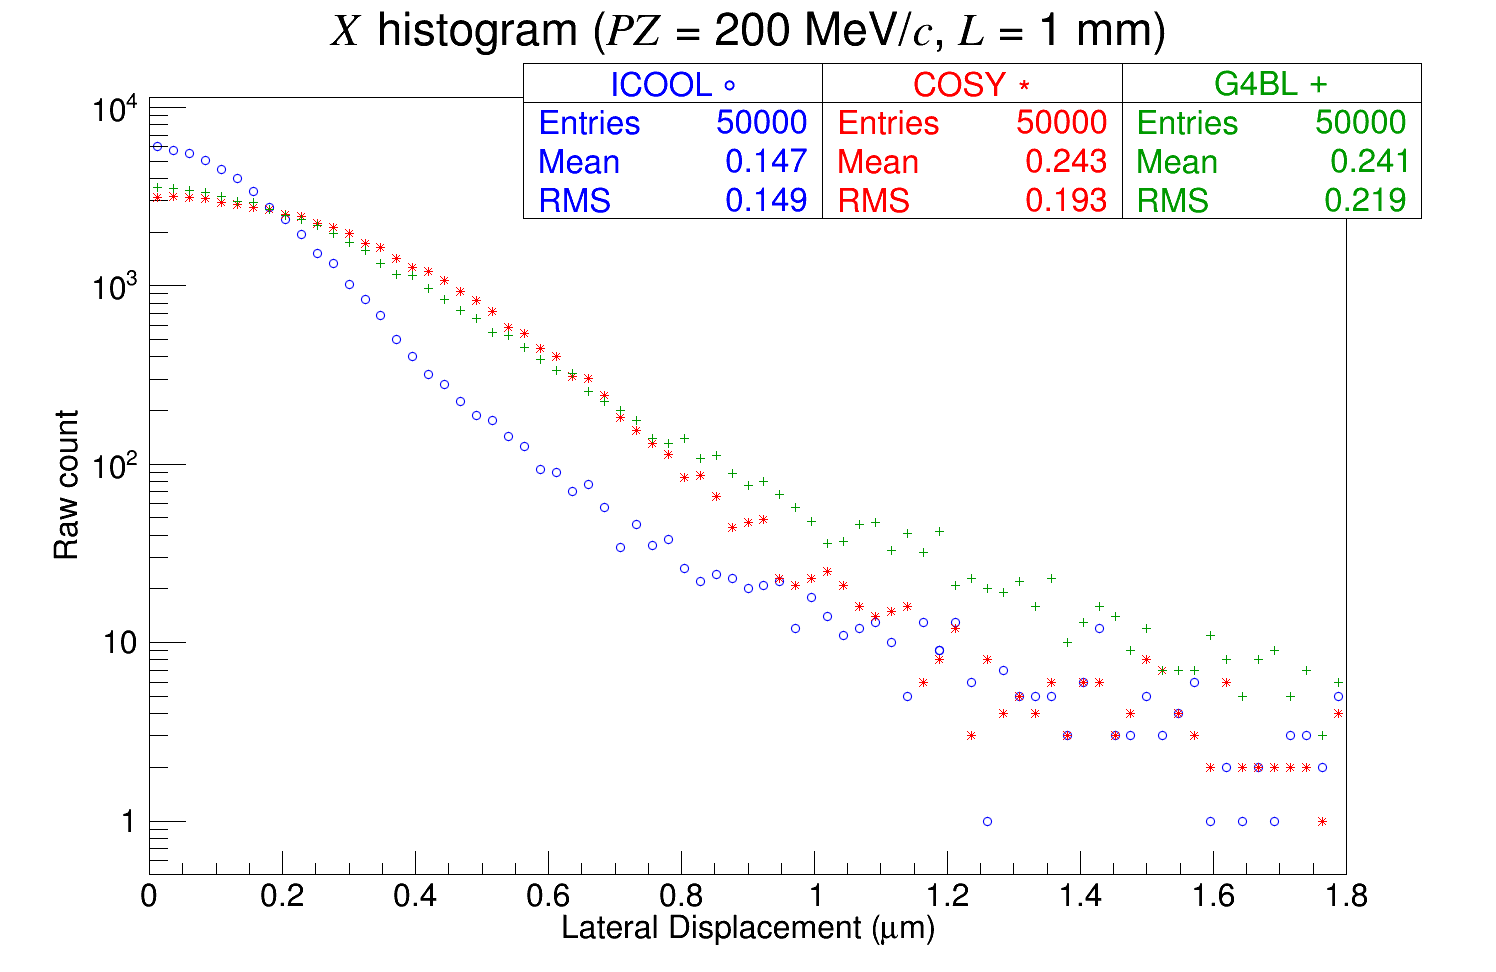
\includegraphics[width=0.7\textwidth]{Benchmarking/LH/X.200.1.png} 
    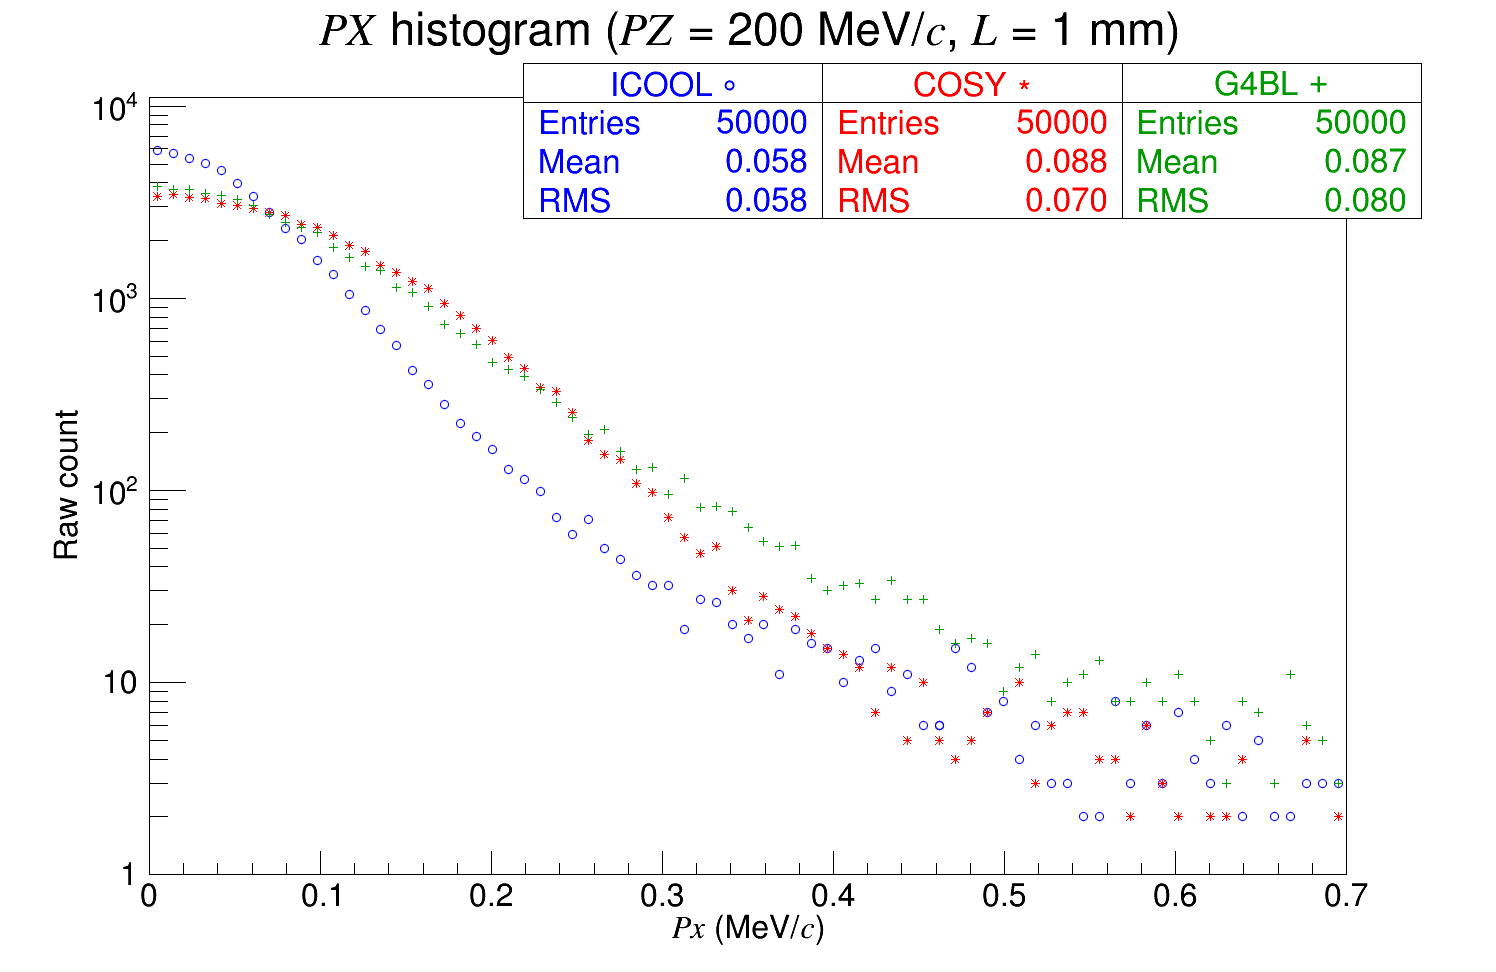
\includegraphics[width=0.7\textwidth]{Benchmarking/LH/PX.200.1.png} 
    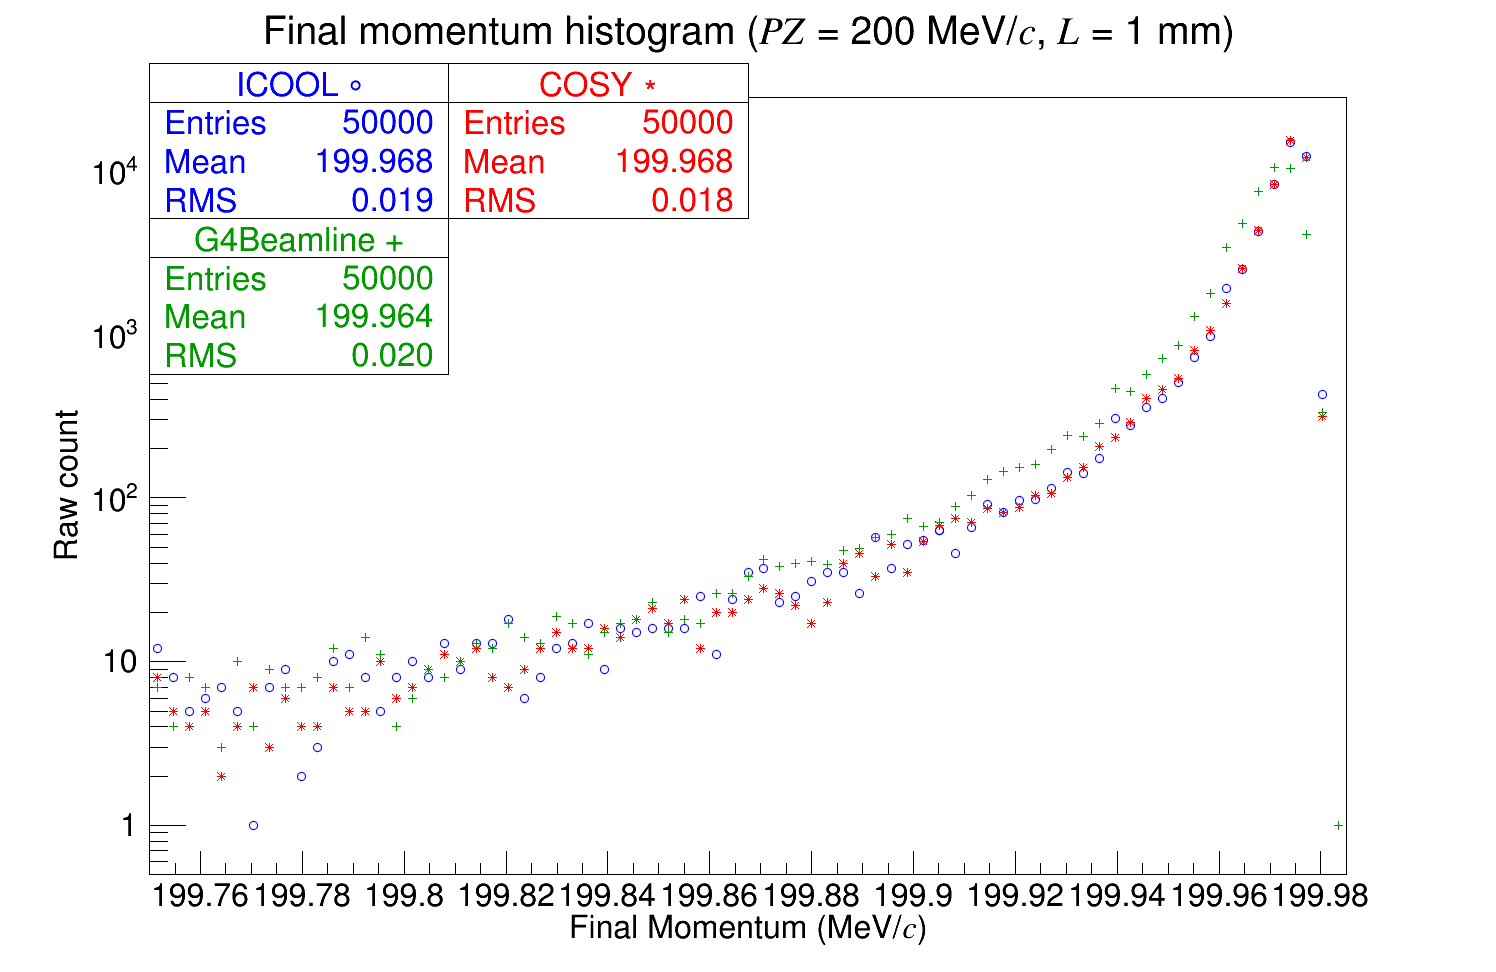
\includegraphics[width=0.7\textwidth]{Benchmarking/LH/strag.200.1.png} 
  \caption[Muons of momentum 200 MeV/$c$ through 1 mm liquid hydrogen.]{Muons of momentum 100 MeV/$c$ through 1 mm liquid hydrogen. Observe that for the $x$ and $p_x$ histograms, COSY and G4beamline follow a Gaussian-like peak whereas ICOOL follows a Fano peak.}
  \label{fig:200.1}
\end{figure}

\begin{figure}[H]
  \centering
    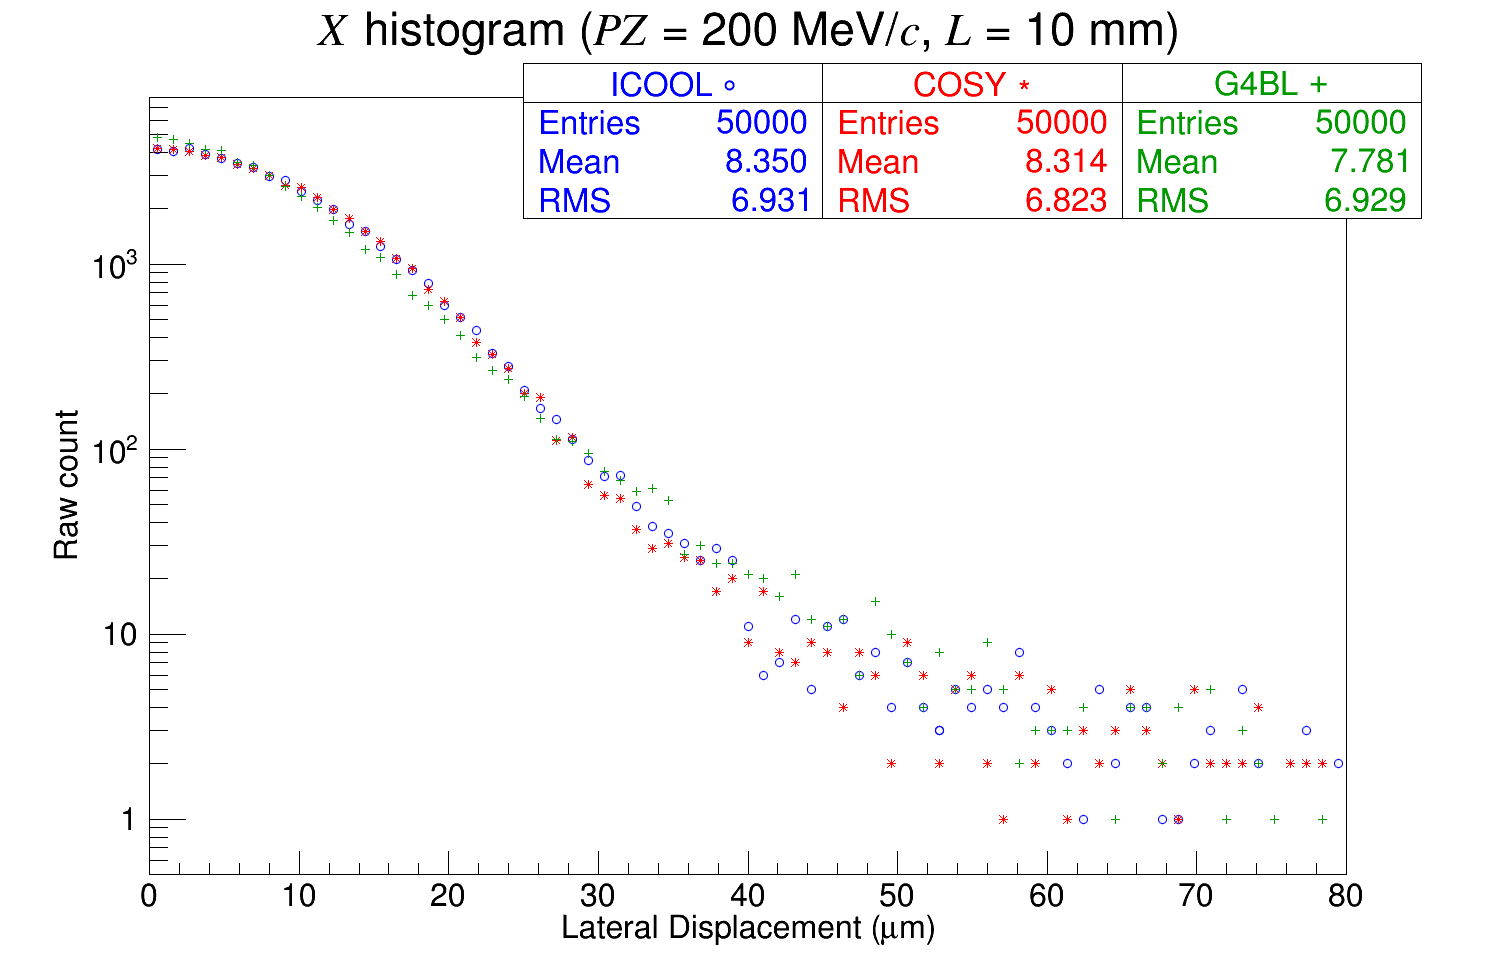
\includegraphics[width=0.7\textwidth]{Benchmarking/LH/X.200.10.png} 
    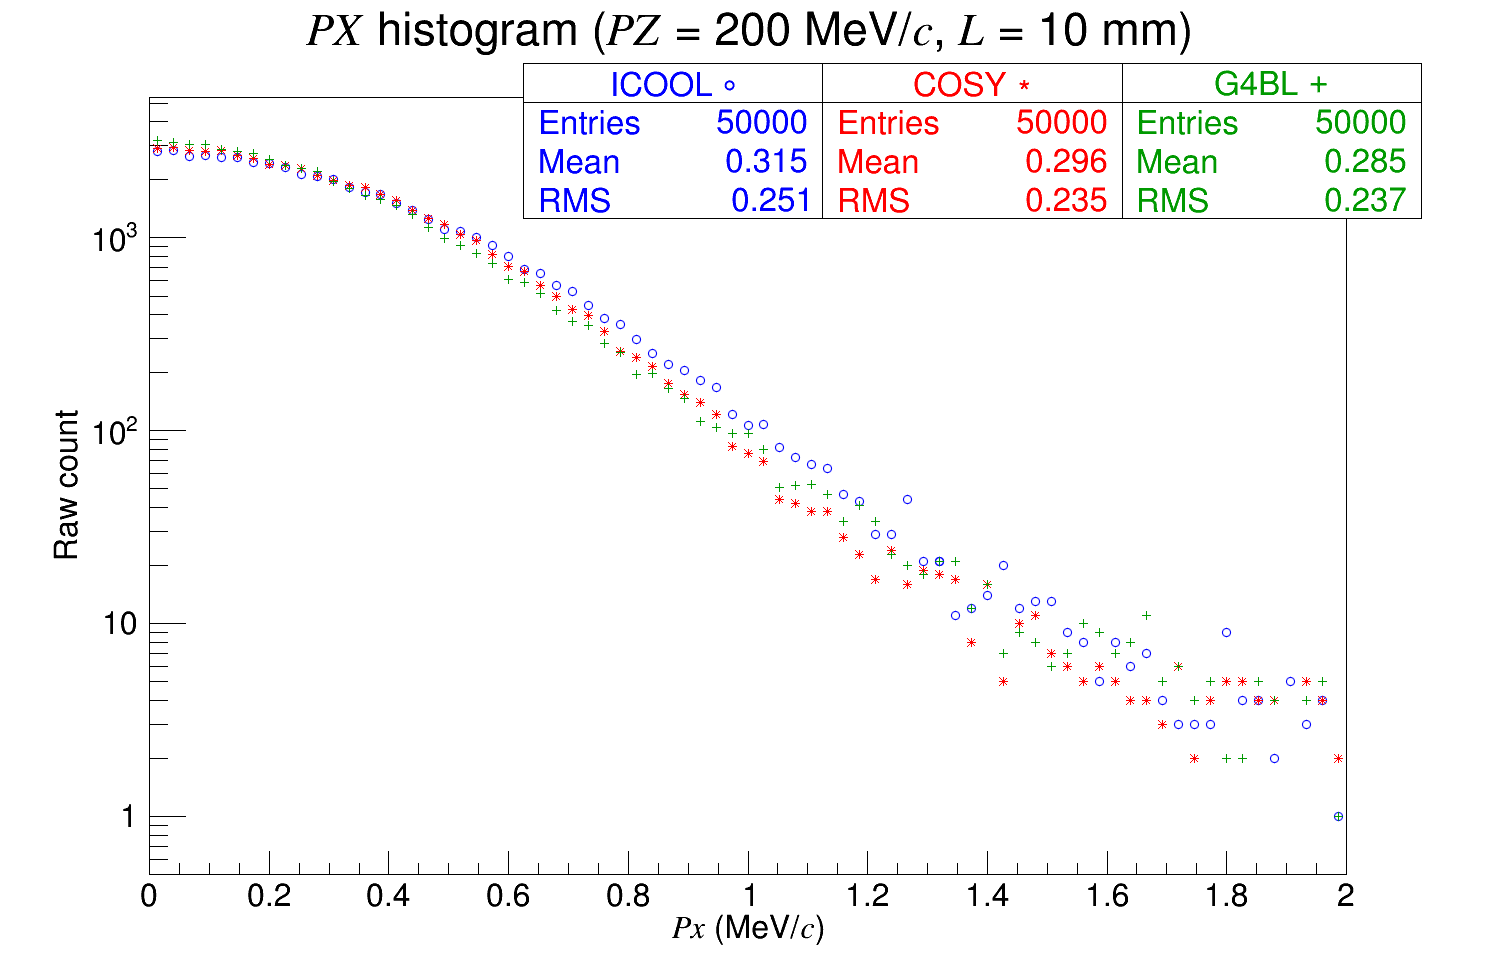
\includegraphics[width=0.7\textwidth]{Benchmarking/LH/PX.200.10.png} 
    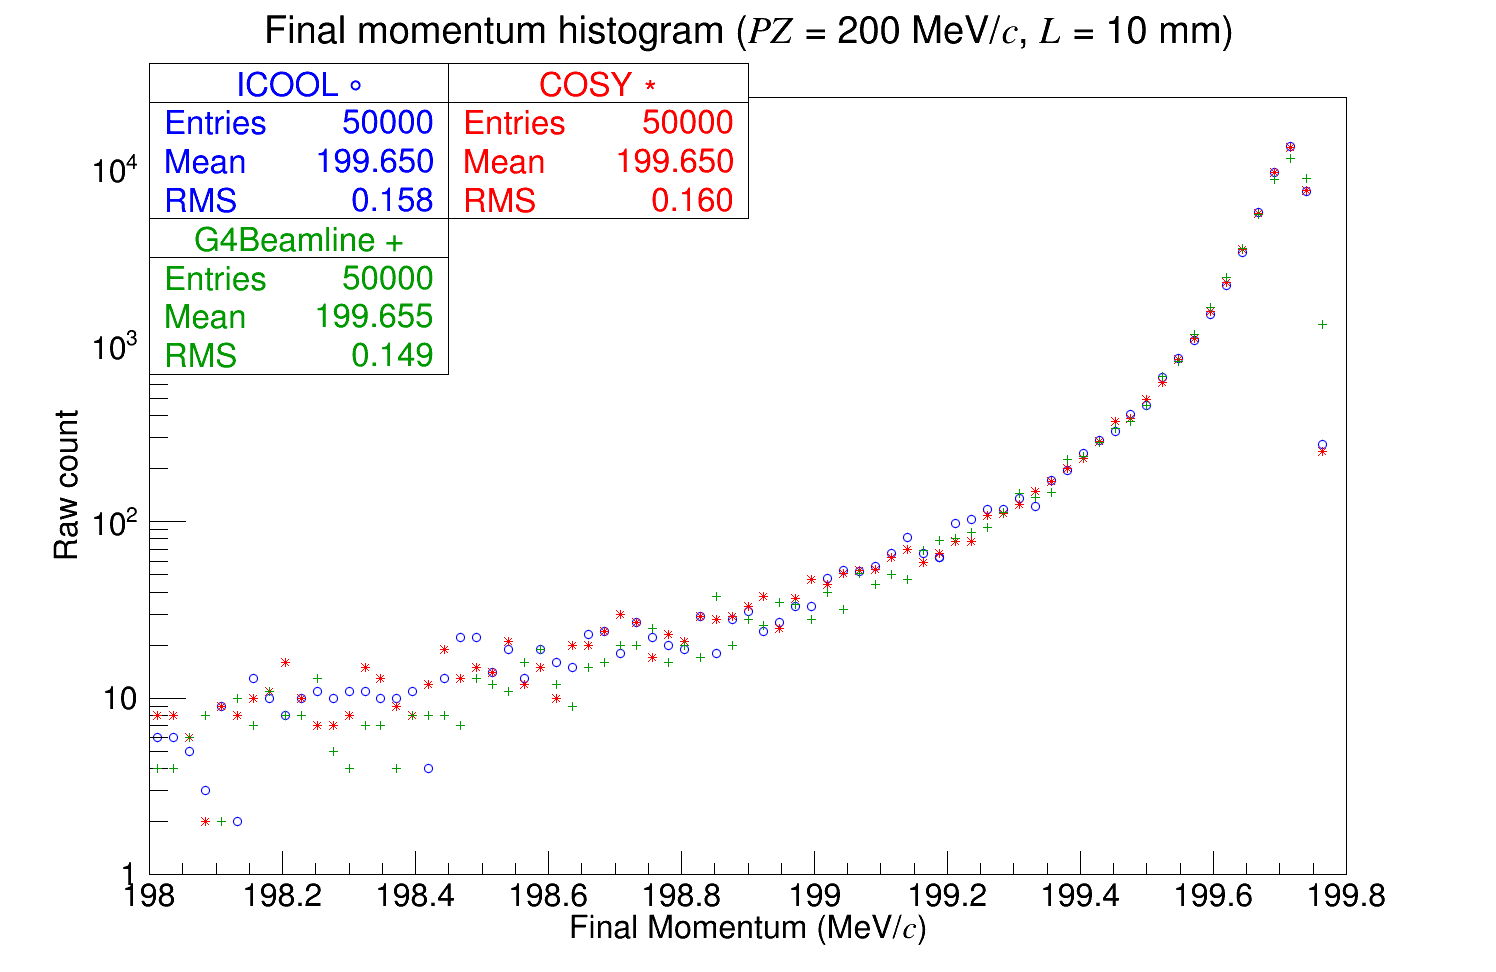
\includegraphics[width=0.7\textwidth]{Benchmarking/LH/strag.200.10.png} 
  \caption{Muons of momentum 200 MeV/$c$ through 10 mm liquid hydrogen.}
  \label{fig:200.10}
\end{figure}

\begin{figure}[H]
  \centering
    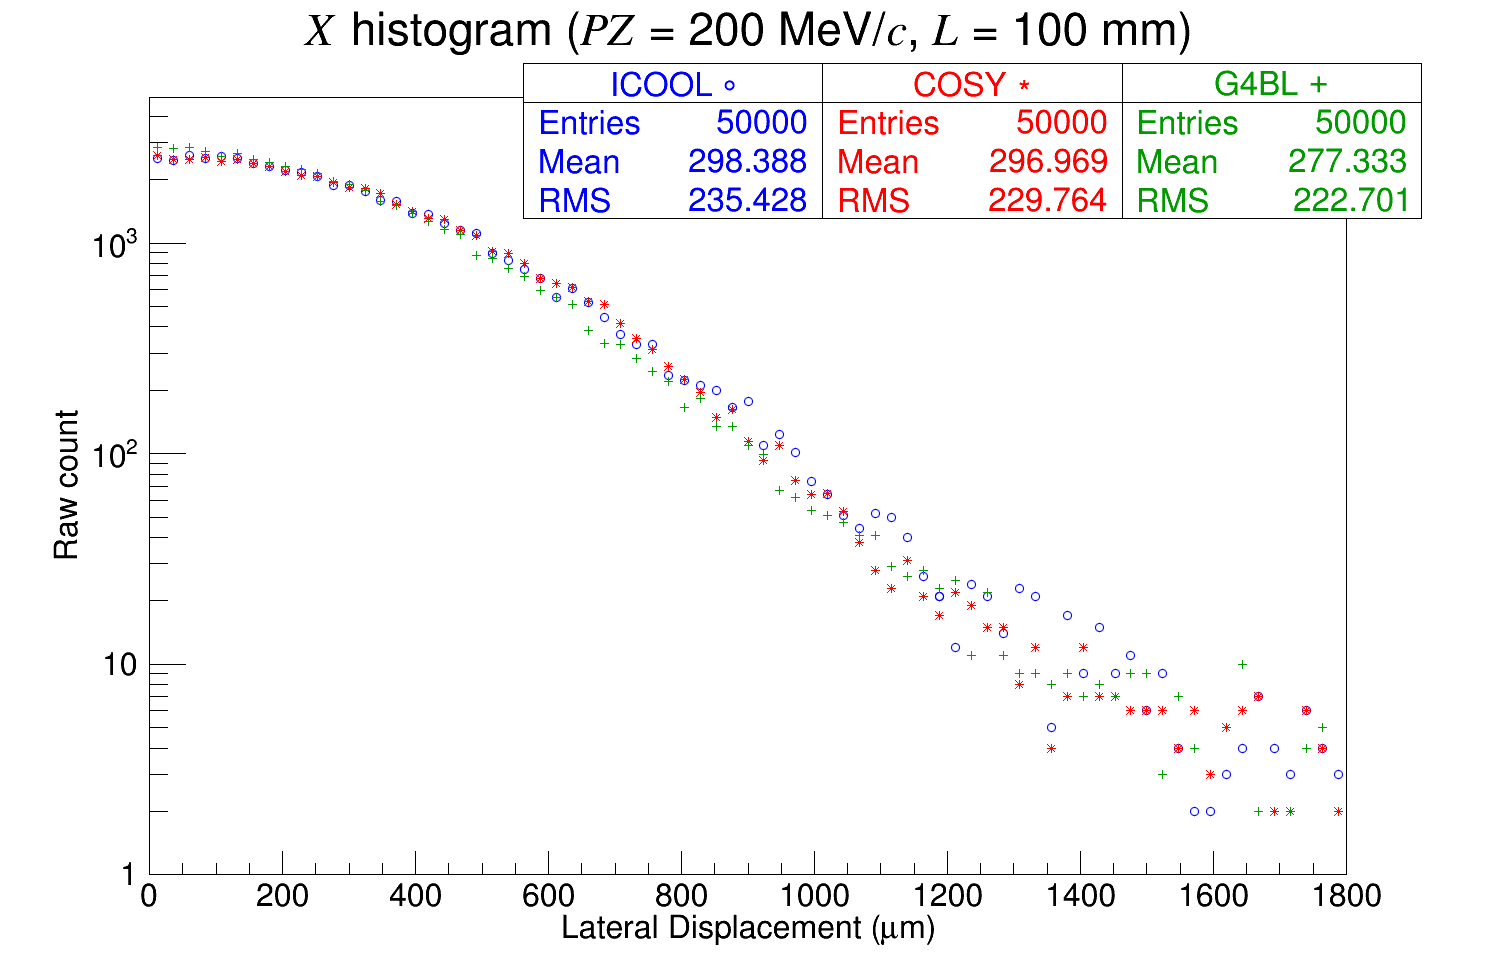
\includegraphics[width=0.7\textwidth]{Benchmarking/LH/X.200.100.png} 
    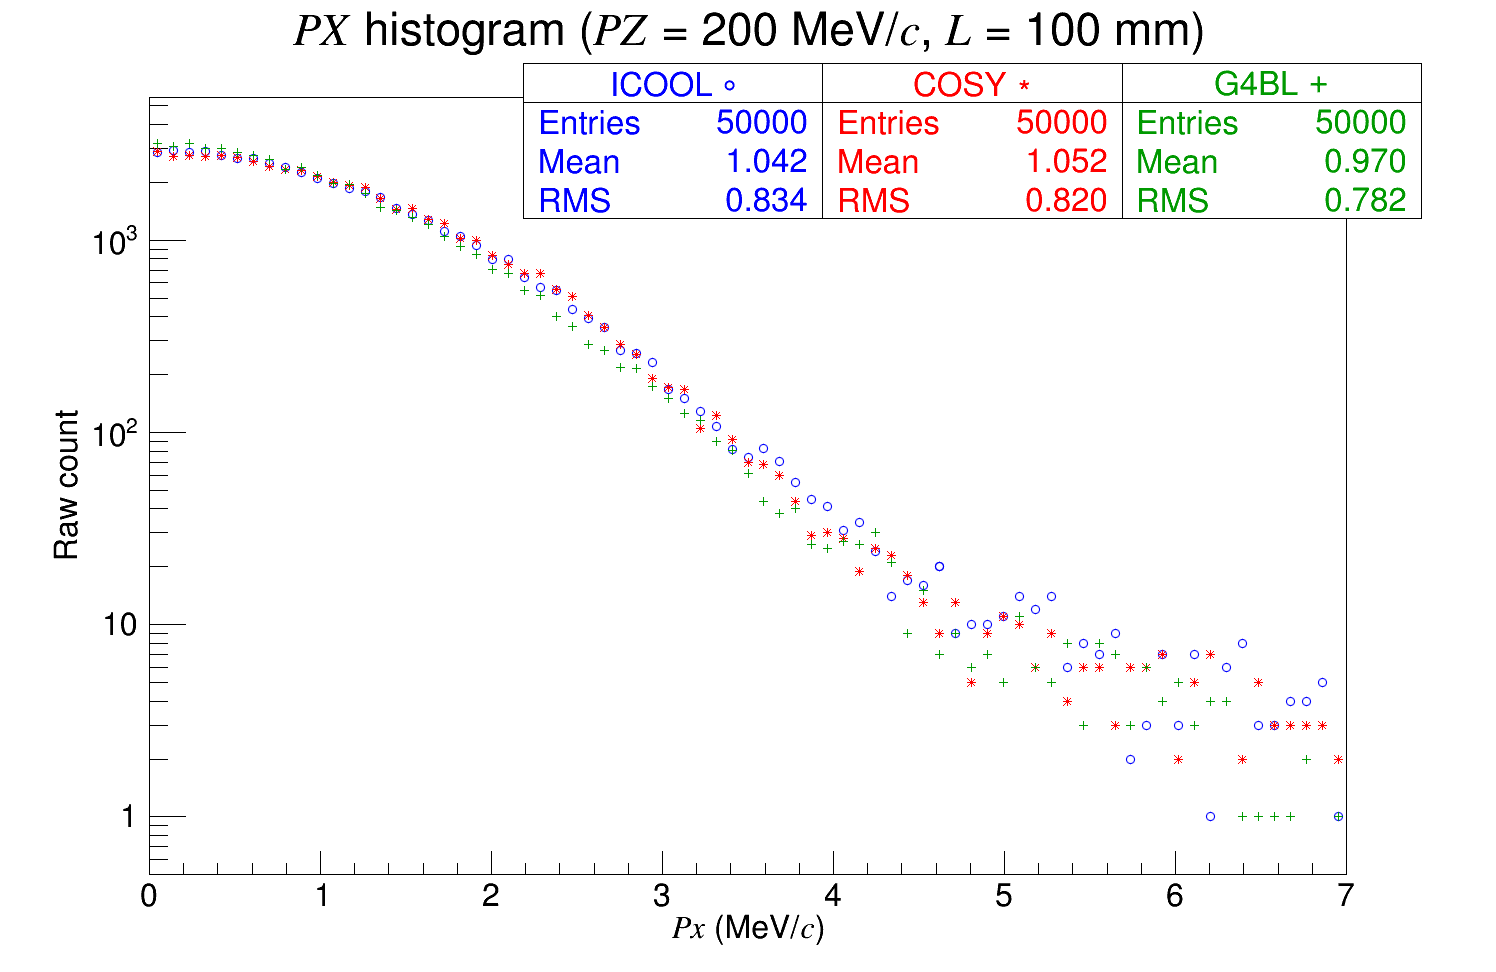
\includegraphics[width=0.7\textwidth]{Benchmarking/LH/PX.200.100.png} 
    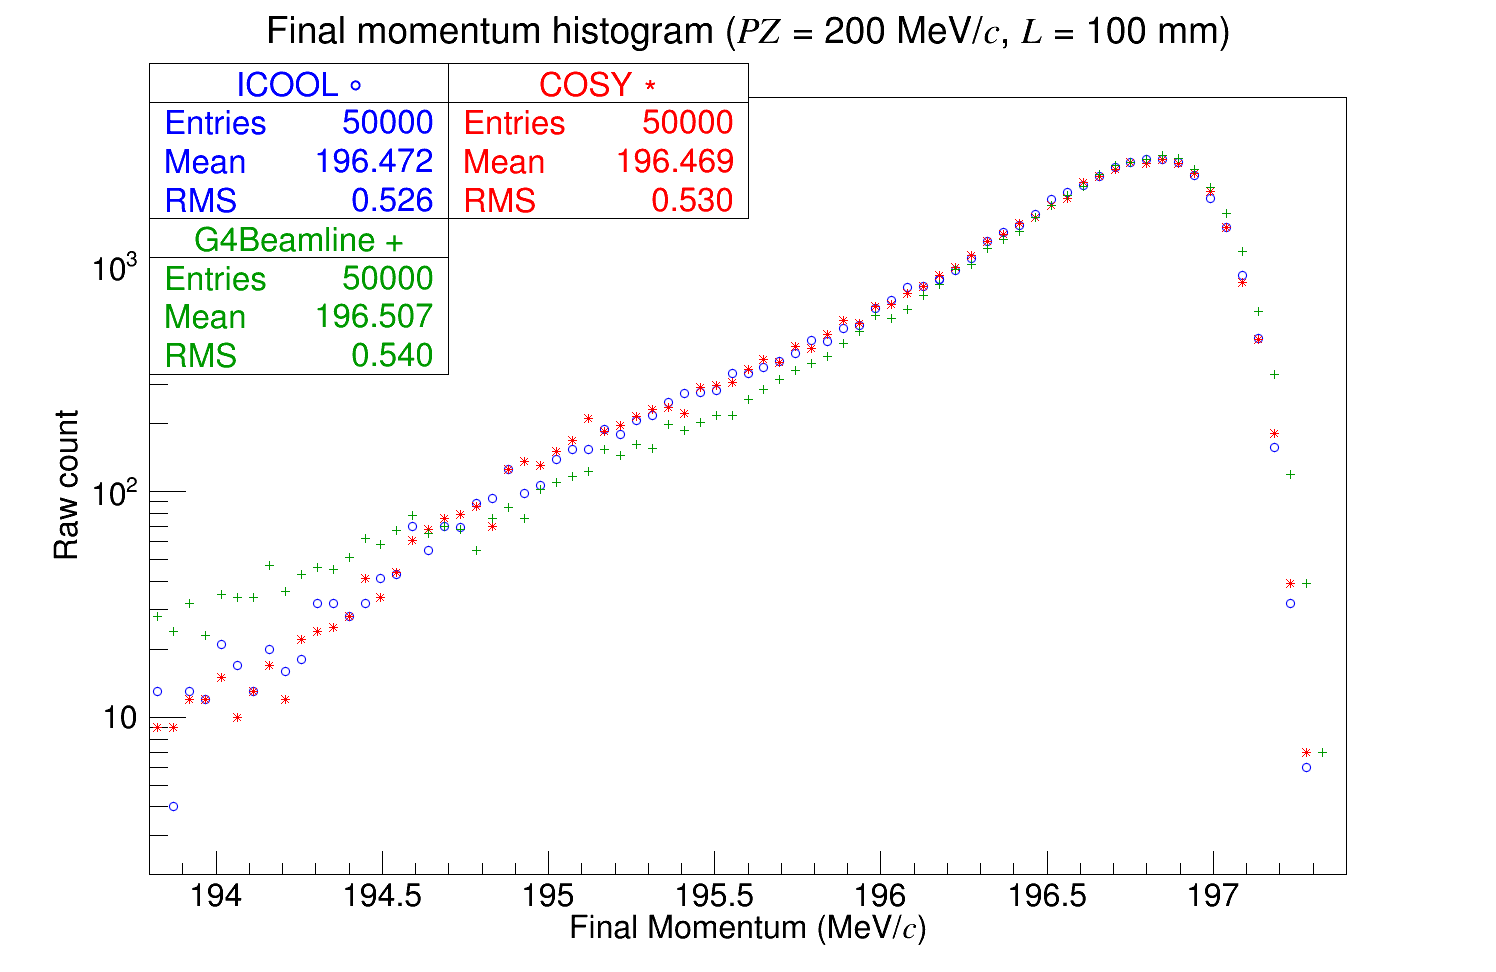
\includegraphics[width=0.7\textwidth]{Benchmarking/LH/strag.200.100.png} 
  \caption{Muons of momentum 200 MeV/$c$ through 100 mm liquid hydrogen.}
  \label{fig:200.100}
\end{figure}

\begin{figure}[H]
  \centering
    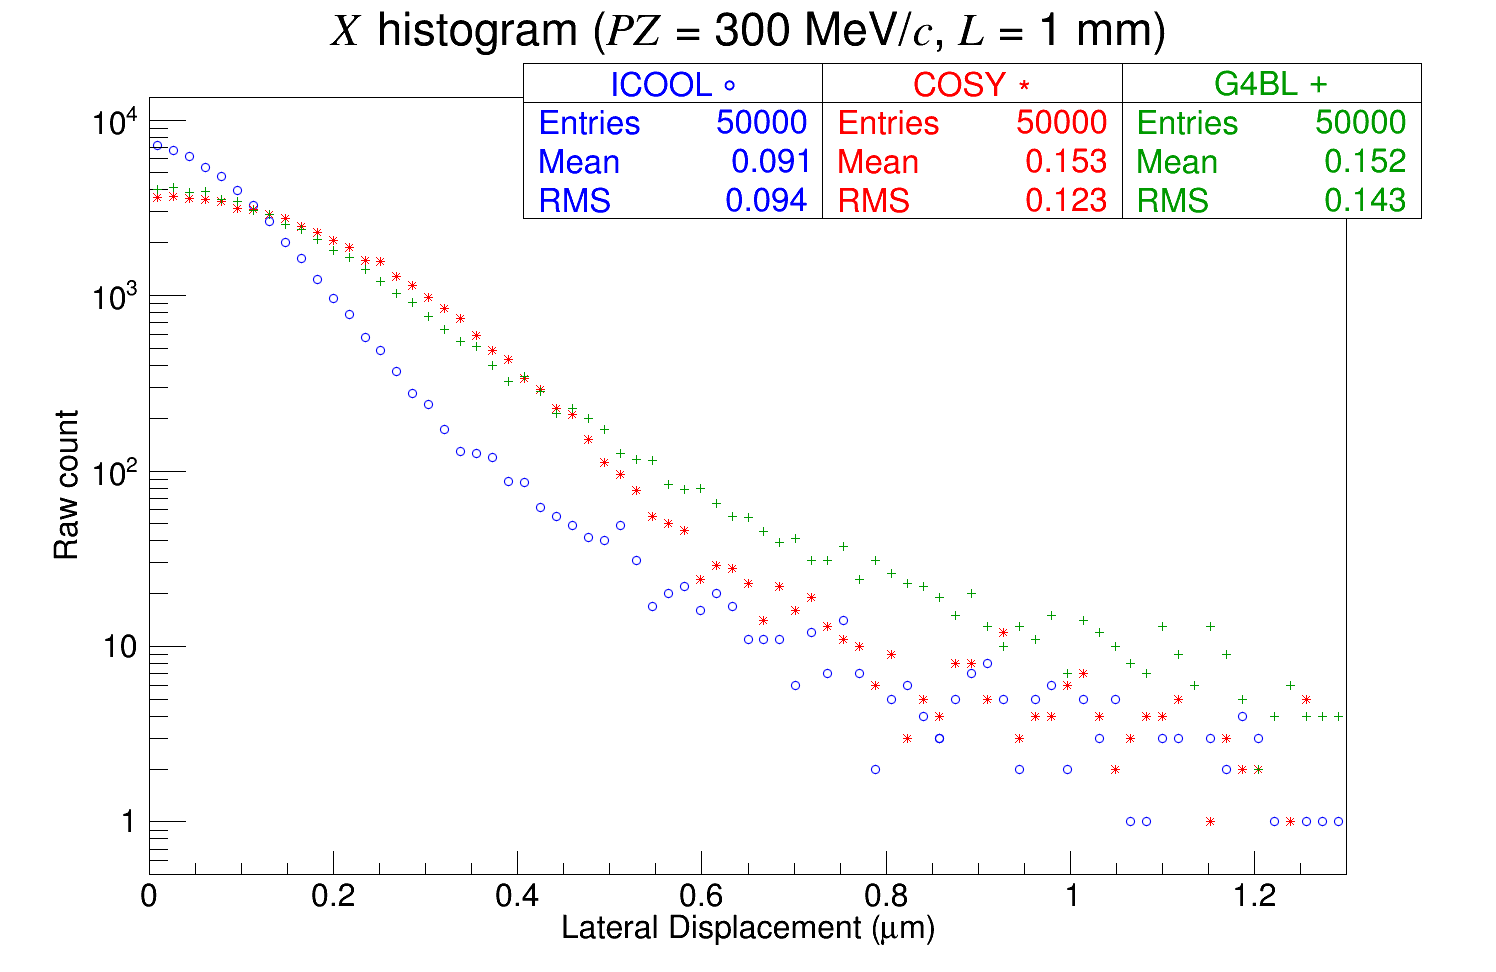
\includegraphics[width=0.7\textwidth]{Benchmarking/LH/X.300.1.png} 
    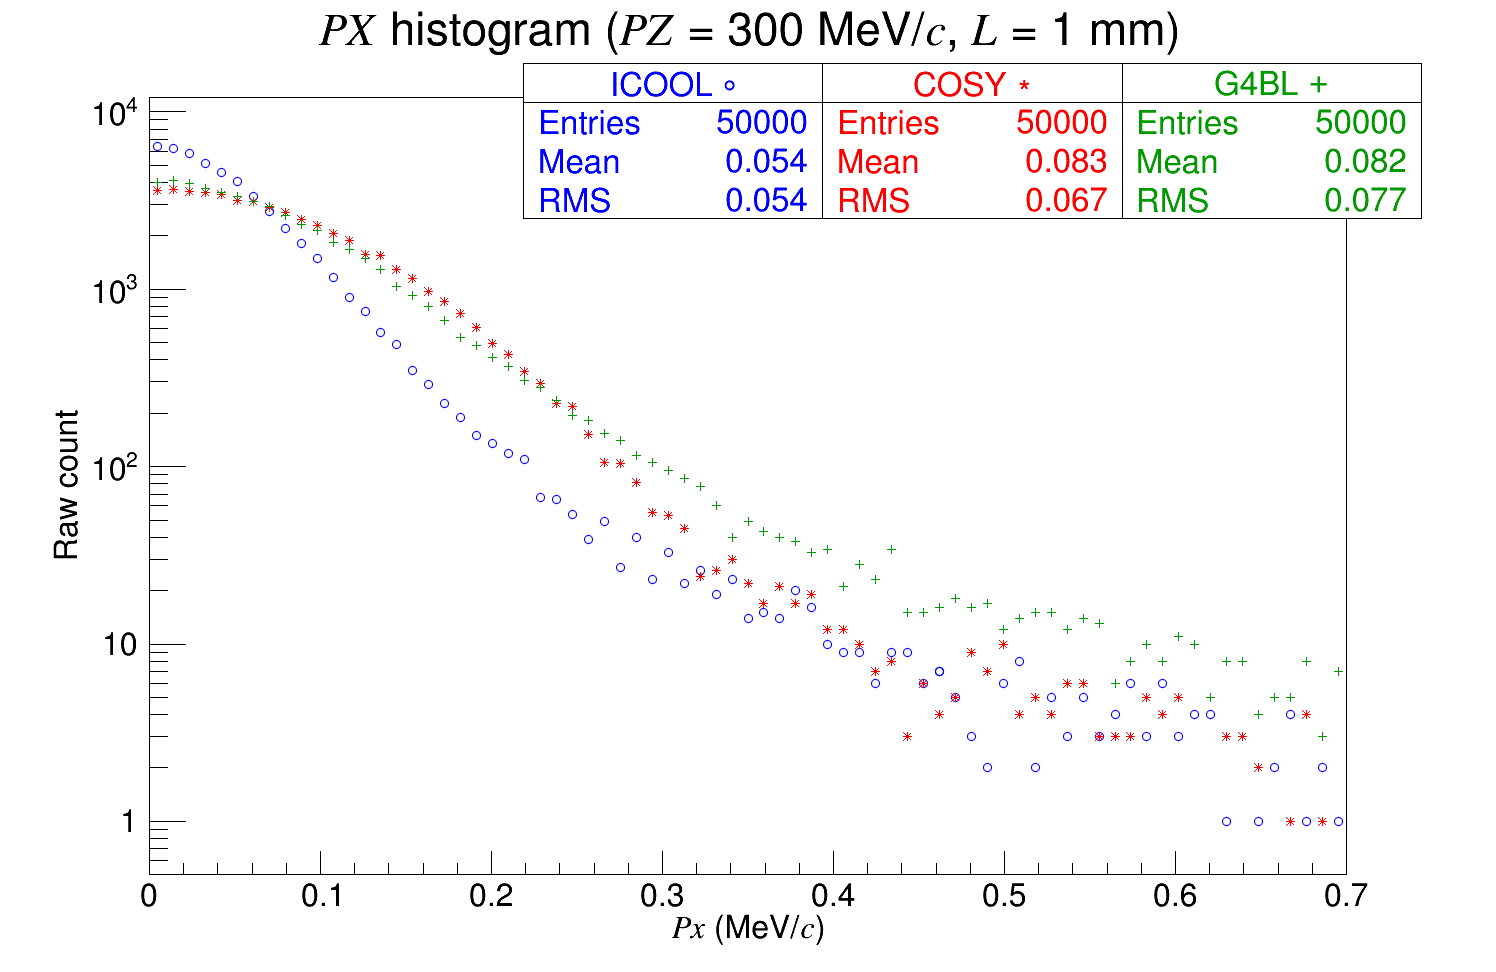
\includegraphics[width=0.7\textwidth]{Benchmarking/LH/PX.300.1.png} 
    \includegraphics[width=0.7\textwidth]{Benchmarking/LH/strag.300.1.png} 
  \caption[Muons of momentum 300 MeV/$c$ through 1 mm liquid hydrogen.]{Muons of momentum 100 MeV/$c$ through 1 mm liquid hydrogen. Observe that for the $x$ and $p_x$ histograms, COSY and G4beamline follow a Gaussian-like peak whereas ICOOL follows a Fano peak.}
  \label{fig:300.1}
\end{figure}


\begin{figure}[H]
  \centering
    \includegraphics[width=0.7\textwidth]{Benchmarking/LH/X.300.10.png} 
    \includegraphics[width=0.7\textwidth]{Benchmarking/LH/PX.300.10.png} 
    \includegraphics[width=0.7\textwidth]{Benchmarking/LH/strag.300.10.png} 
  \caption{Muons of momentum 300 MeV/$c$ through 10 mm liquid hydrogen.}
  \label{fig:300.10}
\end{figure}

\begin{figure}[!htb]
  \centering
    \includegraphics[width=0.7\textwidth]{Benchmarking/LH/X.300.100.png} 
    \includegraphics[width=0.7\textwidth]{Benchmarking/LH/PX.300.100.png} 
    \includegraphics[width=0.7\textwidth]{Benchmarking/LH/strag.300.100.png} 
  \caption{Muons of momentum 300 MeV/$c$ through 100 mm liquid hydrogen.}
  \label{fig:300.100}
\end{figure}

\begin{figure}[H]
  \centering
    \includegraphics[width=0.7\textwidth]{Benchmarking/LH/X.400.1.png} 
    \includegraphics[width=0.7\textwidth]{Benchmarking/LH/PX.400.1.png} 
    \includegraphics[width=0.7\textwidth]{Benchmarking/LH/strag.400.1.png} 
  \caption[Muons of momentum 400 MeV/$c$ through 1 mm liquid hydrogen.]{Muons of momentum 100 MeV/$c$ through 1 mm liquid hydrogen. Observe that for the $x$ and $p_x$ histograms, COSY and G4beamline follow a Gaussian-like peak whereas ICOOL follows a Fano peak.}
  \label{fig:400.1}
\end{figure}

\begin{figure}[H]
  \centering
    \includegraphics[width=0.7\textwidth]{Benchmarking/LH/X.400.10.png} 
    \includegraphics[width=0.7\textwidth]{Benchmarking/LH/PX.400.10.png} 
    \includegraphics[width=0.7\textwidth]{Benchmarking/LH/strag.400.10.png} 
  \caption{Muons of momentum 400 MeV/$c$ through 10 mm liquid hydrogen.}
  \label{fig:400.10}
\end{figure}

\begin{figure}[H]
  \centering
    \includegraphics[width=0.7\textwidth]{Benchmarking/LH/X.400.100.png} 
    \includegraphics[width=0.7\textwidth]{Benchmarking/LH/PX.400.100.png} 
    \includegraphics[width=0.7\textwidth]{Benchmarking/LH/strag.400.100.png} 
  \caption{Muons of momentum 400 MeV/$c$ through 100 mm liquid hydrogen.}
  \label{fig:400.100}
\end{figure}


For the 1 mm figures (Figures \ref{fig:100.1}, \ref{fig:200.1}, \ref{fig:300.1}, and \ref{fig:400.1}) there is much disagreement among the codes' transverse momentum distributions. Since the transverse momentum and transverse position coordinates are related, there is also disagreement among the transverse position distributions. This is likely because the default ICOOL scattering model uses a Fano peak with a Rutherford tail whereas both COSY and G4beamline use a Gaussian peak. It can be seen in, e.g., Figure~\ref{fig:100.1} that COSY, like G4beamline, uses the Gaussian model for the peak but, like ICOOL, then switches to a Rutherford tail.

For the 10 mm figures (Figures \ref{fig:100.10}, \ref{fig:200.10}, \ref{fig:300.10}, and \ref{fig:400.10}), both $x$ and $p_x$ distributions agree well. For COSY, the tail of the distribution falls off slightly faster after approximately 1~MeV/$c$. 

For the final momentum plots, ICOOL and COSY agree quite well. This is not surprising since both codes use Landau theory to describe the energy loss distribution. G4beamline occasionally disagrees, which is expected since G4beamline uses a different model. An example of this can be seen in Figure~\ref{fig:200.1}. However, given the scale of the horizontal axis this disagreement is much smaller than it initially appears.

\Section{Validation}\label{sec:validation}

The new COSY routines were also compared to the Muon Scattering Experiment \cite{muscat}, often referred to as MuScat. This experiment measured the scattering of a beam of collimated muons through seven materials. To emulate this, pencil beams with momentum $P=172$ MeV/$c$ were created in COSY, G4beamline, and ICOOL. The pencil beam consisted of $5\times10^6$ particles and was propagated through 109 mm of liquid hydrogen, 159 mm of liquid hydrogen, and 3.73 mm of beryllium. Liquid hydrogen was chosen to represent muons through long absorbers of low-$Z$ materials. Beryllium, on the other hand, was chosen to represent muons through much thinner and denser media. COSY took a single step through the absorbers while G4BL took a step size of 1 mm. The data points were normalized to the total probability (via Simpson's rule). The probability per radian was then found by dividing the probability of the data point by its angle. The results are shown below.

\begin{figure}[H]
  \centering
    \includegraphics[width=\textwidth]{Figures/172.109.muscat} 
  \caption{MuScat angular scattering results for 109 mm of liquid hydrogen compared against COSY (red), G4BL (green), and ICOOL (blue).}
  \label{fig:172.109.muscat}
\end{figure}

\begin{figure}[H]
  \centering
    \includegraphics[width=\textwidth]{Figures/172.159.muscat} 
  \caption{MuScat angular scattering results for 159 mm of liquid hydrogen compared against COSY (red), G4BL (green), and ICOOL (blue).}
  \label{fig:172.159.muscat}
\end{figure}

\begin{figure}[H]
  \centering
    \includegraphics[width=\textwidth]{Figures/172.3.73.muscat} 
  \caption{MuScat angular scattering results for 3.73 mm of beryllium compared against COSY (red), G4BL (green), and ICOOL (blue).}
  \label{fig:172.3.73.muscat}
\end{figure}

In the liquid hydrogen cases, COSY appears to match both G4beamline and ICOOL very well, as well as the MuScat data points. ICOOL appears to have a sharper peak than either COSY or G4beamline, which can be more easily seen in the 159 mm liquid hydrogen case than in the 109 mm case. In the case of beryllium, COSY matches the MuScat points slightly better than G4beamline and ICOOL, particularly for the two data points between 0.04 and 0.06 radians.

\Section{The Muon Ionization Cooling Experiment}\label{sec:mice}

This section introduces the Muon Ionization Cooling Experiment (MICE, \cite{mice}), a practical application for the new absorber routines in COSY. The results of the MICE simulations in ICOOL, G4beamline, and COSY are examined, showing good agreement.

\Subsection{Introduction to MICE}\label{ssc:miceIntro}
The Muon Ionization Cooling Experiment (MICE \cite{mice}) is an experiment currently in progress at the Rutherford Appleton Laboratory in Oxfordshire, U.K. Its goal is to show a proof-of-principle demonstration of muon ionization cooling. The MICE Step IV configuration is explored in this work. The Step IV cell includes 12 magnetic coils positioned symmetrically around a flat absorber. Figure~\ref{fig:miceStepIV} shows a schematic of this lattice with 350 mm of liquid hydrogen as the absorber.
\begin{figure}[h!]
  \centering
    \includegraphics[width=\textwidth]{Figures/miceStepIV} 
  \caption[MICE Step IV cell.]{MICE Step IV cell. Magnetic coils are shown in yellow and the absorber is shown in blue. The green and blue axes are the $y$ and $z$ axes, here drawn to scale as 500 mm each. The aperture (invisible for display purposes) is 300 mm. Image rendered via G4beamline \cite{g4bl}.}
  \label{fig:miceStepIV}
\end{figure}

\Subsection{Results of the MICE Simulation}\label{ssc:miceResults}
$10^6$ muons were simulated through the cell in Figure~\ref{fig:miceStepIV}. The coil parameters may be found in Table~\ref{tbl:MICE_coil_parameters}. The absorber was a 350 mm cylindrical block\footnote{The cylindrical block geometry is an approximation. It should be noted that a real absorber has a more complicated geometry since it is shaped with curved windows. However, since we are using the same simple geometry in each code, the comparison is valid.} of liquid hydrogen centered at $z=0$. The aperture was set to 300 mm. Note that other materials such as safety windows were not accounted for in this simulation. The decay process was disabled in all simulation codes. The beam started at $-$2.45105 m and ended at 2.450 m. The initial distribution was Gaussian with parameters summarized in Table~\ref{tbl:MICE_initial_distribution_parameters}.

\begin{table}
\caption[MICE Step IV coil parameters.]{MICE Step IV coil parameters corresponding to Figure~\ref{fig:miceStepIV}. Here, the coils are in the so-called ``flip'' mode, where the coil currents downstream have the opposite sign of the coils upstream.}
\begin{center}
\begin{tabularx}{\textwidth}{cccccccc}
\hline \hline
Name & $z$ position & Length & Inner radius & Outer radius & Current density  \vspace{-12pt}\\
 & mm & mm & mm & mm & A/mm$^2$  \\
\hline
	End2 & $\mp$3200.28&110.642&258&325.783&$\pm$126 \vspace{-12pt}\\
	Center&$\mp$2450.275&1314.3&258&280.125&$\pm$148 \vspace{-12pt}\\
	End1 & $\mp$1700.29& 110.642& 258 & 318.905 & $\pm$133 \vspace{-12pt}\\
	Match2 & $\mp$1300.29 & 199.492 & 258 & 288.925 & $\pm$132 \vspace{-12pt}\\
	Match1 & $\mp$860.645 & 201.268 & 258 & 304.165 & $\pm133$ \vspace{-12pt}\\
	Focus & $\mp$202.2 & 213.3 & 267.6 & 361.9 & $\pm$104 \\ 
\hline
\end{tabularx}
\end{center}
\label{tbl:MICE_coil_parameters}
\end{table}

%\newcolumntype{A}{ >{\centering\arraybackslash} m{2.5cm} } 
\begin{table}
\caption{MICE Step IV initial distribution Gaussian parameters.}
\begin{center}
\begin{tabularx}{0.7\textwidth}{p{1cm}ccc}
\hline \hline
&Parameter & Mean & Standard deviation \\
\hline
	&$x$ (mm) & 0 & 32\vspace{-12pt}\\
	&$y$ (mm) & 0 & 32\vspace{-12pt} \\
	&$z$ (mm) & 0 & 0\vspace{-12pt} \\
	&$p_x$ (MeV/$c$) & 0 & 20\vspace{-12pt} \\
	&$p_y$ (MeV/$c$) & 0 & 20\vspace{-12pt} \\
	&$p_z$ (MeV/$c$) & 200 & 30\\
\hline
\end{tabularx}
\end{center}
\label{tbl:MICE_initial_distribution_parameters}
\end{table}

While the selection of order and step size is detailed in the next section, it was found that a 5th order simulation was sufficient for COSY. Through the coil-only portion of the simulation, 50 steps were taken on each side of the absorber (or roughly a step size of 46 mm both upstream and downstream). The particles were tracked through the succession of transfer maps corresponding to individual steps. It was noted that for the coil-only section, a single transfer map was not sufficient even at the 9th order. This is due to the relatively large phase space volume of the beam and the complexity of the magnetic field. Through the absorber-coil region ($-$350/2 mm to 350/2 mm), it was found that a 1st order map with 5 steps was sufficient. This is due to the transverse phase space of the beam passing through a focal point and the magnetic field passing through the point of symmetry.

Compounding the map without propagating the beam also gave poor results. When one takes the composition of two $n^{th}$ order transfer maps, a transfer map of order $n\times n$ is the result. For example, the first step in the MICE simulation would yield a 5th order transfer map. Taking the second step would give a new transfer map of order $5\times 5 = 25$. However, since COSY is operating in the 5th order mode, the new transfer map would not be 25th order, but rather it would be truncated to a 5th order map. For this reason, the particles were propagated through the momentary transfer map after each step in the simulation.

The magnetic field in G4beamline was created using the \texttt{coil} and \texttt{solenoid} commands. The field was then exported to a file using the \texttt{printfield} command to a file. The field map file was read by both G4beamline (which used the \texttt{fieldmap} command) and ICOOL (which used the \texttt{GRID} command operating in \texttt{G43D} mode).

The results of the simulation represented by Figure~\ref{fig:miceStepIV} can be seen in Figures~\ref{fig:micex} through~\ref{fig:miceenergy}. It can be seen that all three codes agree to within 1\%.

\begin{figure}[H]
  \centering
    \includegraphics[width=\textwidth]{MICE data/x} 
  \caption{MICE Step IV $x$ position results for 350 mm of liquid hydrogen.}
  \label{fig:micex}
\end{figure}

\begin{figure}[H]
  \centering
    \includegraphics[width=\textwidth]{MICE data/px} 
  \caption{MICE Step IV $x$ angle results for 350 mm of liquid hydrogen.}
  \label{fig:micexangle}
\end{figure}

\begin{figure}[H]
  \centering
    \includegraphics[width=\textwidth]{MICE data/e} 
  \caption{MICE Step IV final energy results for 350 mm of liquid hydrogen.}
  \label{fig:miceenergy}
\end{figure}

The runtimes of ICOOL, G4beamline, and COSY are listed in Table~\ref{tbl:mice_times}. To reiterate, COSY was run at 5th order with 50 steps before the absorber, 5 steps at 1st order inside the absorber, and 50 steps at 5th order after the absorber. Note that the initialization time for G4beamline to create the field maps was 33 seconds. The time it took to create a text file for ICOOL input was 11 seconds. Since G4beamline only has to create the field map once, the initialization time is added to neither the ICOOL nor G4beamline run times in Table~\ref{tbl:mice_times}. COSY did not have any initialization time.

\begin{table}
\caption[Run times for the MICE Step IV simulation.]{Run times for the MICE Step IV simulation for liquid hydrogen. Note that the G4beamline initialization time was not added to the run time values. G4BL (coils) represents the simulation in G4beamline when the \texttt{coil} parameter was used. G4BL (field map) represents the simulation when G4beamline (like ICOOL) read the field map from a file.}
\begin{center}
\begin{tabularx}{0.55\textwidth}{ccccc}
%\vspace{-40pt}\\ 
\hline \hline
Number of particles: & $10^6$ & $10^5$ & $10^4$ & $10^3$\\
\hline
COSY: & 367 & 31 & 6 & 4\vspace{-12pt}\\
G4BL (coils): & 3973 & 392 & 40 & 6\vspace{-12pt}\\
G4BL (field map): & 662 & 75 & 15 & 9\vspace{-12pt}\\
ICOOL (field map): & 1091 & 117 & 19 & 9\\
\hline
\end{tabularx}
\end{center}
\label{tbl:mice_times}
\end{table}

As a second test, the MICE configuration in Figure~\ref{fig:miceStepIV} was simulated using 65 mm of lithium hydride. Lithium hydride is an attractive material because, unlike liquid hydrogen, it does not require cryogenic conditions, but still maintains a low $Z$ value. It can be seen from Figures \ref{fig:mice_lih_x}, \ref{fig:mice_lih_xangle}, and \ref{fig:mice_lih_energy} that 65 mm of lithium hydride has a similar effect on the beam as 350 mm of liquid hydrogen.

\begin{figure}[H]
  \centering
    \includegraphics[width=\textwidth]{MICE data/LiH/x} 
  \caption{MICE Step IV $x$ position results for 65 mm of lithium hydride.}
  \label{fig:mice_lih_x}
\end{figure}

\begin{figure}[H]
  \centering
    \includegraphics[width=\textwidth]{MICE data/LiH/px} 
  \caption{MICE Step IV $x$ angle results for 65 mm of lithium hydride.}
  \label{fig:mice_lih_xangle}
\end{figure}

\begin{figure}[H]
  \centering
    \includegraphics[width=\textwidth]{MICE data/LiH/e} 
  \caption{MICE Step IV final energy results for 65 mm of lithium hydride.}
  \label{fig:mice_lih_energy}
\end{figure}

\Subsection{Step Size Effects}\label{ssc:step_size_effects}
Several step sizes were tested in COSY to ensure optimal efficiency. The results are discussed here.

For the absorber-coil section of the MICE liquid hydrogen lattice ($-$350/2 mm to 350/2 mm), it was found that 5 steps were sufficient to approximate the superposition of the absorber and coils. To study this step size dependence, $10^5$ particles from the initial distribution found in Table~\ref{tbl:MICE_initial_distribution_parameters} were propagated through the 350 mm liquid hydrogen flat absorber. This simulation took the surrounding magnetic fields into account. Table~\ref{tbl:mice_step_size_ac} shows the effect of changing the step size for the absorber-coil section only.

\begin{table}
\caption[Step size dependence for the absorber-coil section of the MICE Step IV lattice for liquid hydrogen.]{First order step size dependence for the absorber-coil section of the MICE Step IV lattice for $10^5$ muons passing through 350 mm of liquid hydrogen. The transmission was very nearly 100\% for all three codes regardless of circumstances. The energy for COSY does not change much with respect to order since the energy loss algorithm does not use a transfer map approach.}
\begin{center}
\begin{tabularx}{\textwidth}{cccccc}
\hline \hline
& ICOOL & G4BL & \multicolumn{3}{c}{\sout{\hspace{1.5cm}} COSY \sout{\hspace{1.5cm}}}\\
& (field map) & (field map) & 1 step & 5 steps & 10 steps\\
\hline
$\sigma_x$ (mm): & 50.5 & 50.4 & 50.3 & 50.6 & 50.7\\
$\sigma_{\theta_x}$ (mrad): & 201.9 & 201.4 & 205.7 & 200.5 & 199.9\\
$\sigma_E$ (MeV): & 26.7 & 26.7 & 26.6 & 26.6 & 26.6\\
Computational time (s): & 19 & 25 & 4 & 5 & 8\\
\hline
\end{tabularx}
\end{center}
\label{tbl:mice_step_size_ac}
\end{table}

The discrepancy of COSY w.r.t.\ G4beamline is $<$1\% for all components. Results of the absorber-coil simulation can be seen in Figures \ref{fig:acx}-\ref{fig:ace}. There is good agreement between ICOOL, G4beamline, and COSY.

\begin{figure}[H]
  \centering
    \includegraphics[width=0.7\textwidth]{MICE data/absorber coils/x} 
  \caption{Absorber-coil simulation results for $x$ with $10^5$ muons and a 5 step propagation.}
  \label{fig:acx}
\end{figure}

\begin{figure}[H]
  \centering
    \includegraphics[width=0.7\textwidth]{MICE data/absorber coils/px} 
  \caption{Absorber-coil simulation results for $\theta_x$ with $10^5$ muons and a 5 step propagation.}
  \label{fig:acpx}
\end{figure}

\begin{figure}[H]
  \centering
    \includegraphics[width=0.7\textwidth]{MICE data/absorber coils/e} 
  \caption{Absorber-coil simulation results for the final energy with $10^5$ muons and a 5 step propagation.}
  \label{fig:ace}
\end{figure}

For both the upstream and downstream sections, the entire MICE cell was simulated ($-2.45105$ m to $2.450$ m). It was found that COSY operated sufficiently well at order 5 and with 50 steps in the simulation.

To study this step size dependence, $10^5$ particles from the initial distribution found in Table~\ref{tbl:MICE_initial_distribution_parameters} were propagated through the MICE cell. Table~\ref{tbl:mice_step_size_upstream} shows the effect of changing the step size.

\begin{table}
\caption[Step size dependence for the MICE Step IV lattice.]{Step size dependence for the MICE Step IV lattice for $10^5$ muons. The notation for COSY is [order]@[number of steps].}
\begin{center}
\begin{tabularx}{\textwidth}{cccccccc}
\hline \hline
& ICOOL & G4BL & \multicolumn{5}{c}{COSY [order]@[number of steps]}\vspace{-12pt}\\
& (field map) & (field map) & 3@50 & 5@30 & 5@50 & 5@100 & 7@100\\
\hline
$\sigma_x$ (mm): & 40.7 & 40.7 & 42.5 & 41.2 & 41.4 & 41.4 & 41.0\\
$\sigma_{\theta_x}$ (mrad): & 240.2 & 240.2 & 248.3 & 239.8 & 242.1 & 243.8 & 241.8\\
\% transmission: & 98.5 & 98.5 & 99.6 & 96.8 & 97.7 & 98.6 & 97.9\\
Comp. time (s): & 114 & 82 & 12 & 21 & 25 & 43 & 132\\
\hline
\end{tabularx}
\end{center}
\label{tbl:mice_step_size_upstream}
\end{table}

For most COSY cases, the discrepancy w.r.t.\ G4beamline is on the order of 1\%. 5th order at 50 steps was selected as ``best'' because of the increased agreement with both ICOOL and G4beamline when compared to both 3@50 and 5@30 (particularly for the transmission). Moreover, 5@50 gives similar results as 7@100 but with drastically decreased computational time. 

Results of the step size study for 5@50 can be seen in Figures \ref{fig:upx} and \ref{fig:uppx}. There is good agreement between ICOOL, G4beamline, and COSY.

\begin{figure}[H]
  \centering
    \includegraphics[width=0.7\textwidth]{MICE data/upstream/x} 
  \caption{MICE simulation results for $x$ with $10^5$ muons at 5th order and 50 steps.}
  \label{fig:upx}
\end{figure}

\begin{figure}[H]
  \centering
    \includegraphics[width=0.7\textwidth]{MICE data/upstream/px} 
  \caption{MICE simulation results for $\theta_x$ with $10^5$ muons at 5th order and 50 steps.}
  \label{fig:uppx}
\end{figure}

\Section{Summary}\label{sec:summary}

In summary, new simulation tools for muon ionization cooling have been added to COSY Infinity for particle-by-particle propagation. The energy straggling, multiple scattering, transverse position, and time-of-flight models were developed from first principles. The algorithms implemented have been modified via empirical fit to MuScat \cite{muscat} while keeping a reasonable agreement with G4beamline. Fitted with this new software, COSY has simulated one of the current muon ionization cooling efforts, MICE Step IV \cite{mice}, yielding agreement within 1\% of both ICOOL and G4beamline. The code developed in this work is accurate, fast, and user-friendly.

\appendix
\Appendix{Derivation of Transverse Emittance} \label{apx:emittance}

The following is a derivation of Eq. \eqref{eqn:emittancedef}. First, it is assumed that the beam is an on-axis Gaussian beam. Explicitly, this is to say that the distribution of transverse coordinates is Gaussian and that $\left(\left<x\right>,\left<\theta\right>\right)=(0,0)$. Recall that emittance is a measure of phase space volume. To measure this volume, it is necessary to use a bivariate Gaussian distribution.

In general, a multivariate Gaussian distribution has the form
\begin{equation}\nonumber
f_n (X)=\frac{1}{(2\pi)^{n/2}|\mathcal{A}|^{1/2}}\exp\left(-\frac{1}{2}(X-\mu)^T\mathcal{A}^{-1}(X-\mu)\right),
\end{equation}
where $X=(x_1,...,x_n)$ is a column vector of independent variables, $\mathcal{A}\in S^n_{++}$ is the covariance matrix, and $\mu=(\mu_1,...,\mu_n)$ is a column vector of average values (which are all zero for this derivation) \cite{Do}. $S^n_{++}$ is the space of symmetric positive definite $n\times n$ matrices.  The covariance matrix $\mathcal{A}$ is a matrix that describes the covariance between variables. That is, $\mathcal{A}$ describes how much two given variables change with one another.

As an example, consider the univariate Gaussian distribution. The only variable is $x$ and it changes with itself as $\left<x\cdot x\right> = \sigma^2$. Then
\begin{align*}
X=x,\qquad\mathcal{A}=\sigma^2,
\end{align*}
and
\begin{align*}
f_1 (X)&=\frac{1}{(2\pi)^{1/2}\sigma} \exp\left(-\frac{1}{2}x\frac{1}{\sigma^2}x\right)\\
&=\frac{1}{\sqrt{2\pi}\sigma} \exp\left(-\frac{x^2}{2\sigma^2}\right).
\end{align*}

For the transverse emittance, there are two varibles, $x$ and $\theta$. They change with themselves as their respective $\sigma^2$ and with one another as $\left<x\theta\right>$, and so
\begin{align*}
X=(x,\theta)\qquad\mathcal{A}=\begin{pmatrix}
					\sigma_x^2 & \left<x\theta\right>\\
					\left<x\theta\right> & \sigma_\theta^2
					\end{pmatrix}.
\end{align*}

The distribution is
\begin{align*}
f_2(X)&=\frac{1}{2\pi\sqrt{\sigma_x^2\sigma_\theta^2-\left<x\theta\right>^2}}\exp\left(-\frac{x^2\sigma_\theta^2-2x\theta\left<x\theta\right>+\theta^2\sigma_x^2}{2(\sigma_x^2\sigma_\theta^2-\left<x\theta\right>^2)}\right).
\end{align*}
Since the boundary of this function is undefined, it is conventional to use a metric called the Mahalanobis distance \cite{mahalanobis}. This is a measure of how far some point is away from the center of a multivariate distribution. For a bivariate Gaussian distribution, it is
\begin{align*}
\text{distance}=\frac{1}{2}(X-\mu)^T\mathcal{A}^{-1}(X-\mu)=\frac{x^2\sigma_\theta^2-2x\theta\left<x\theta\right>+\theta^2\sigma_x^2}{2(\sigma_x^2\sigma_\theta^2-\left<x\theta\right>^2)}.
\end{align*} 
As it pertains to emittance, the boundary of interest is all $x$ and $\theta$ combinations which are unit distance from the central peak. Then
\begin{align*}
1=\frac{x^2\sigma_\theta^2-2x\theta\left<x\theta\right>+\theta^2\sigma_x^2}{2(\sigma_x^2\sigma_\theta^2-\left<x\theta\right>^2)}.
\end{align*}

Now it is apparent that this equation represents an ellipse in $x-\theta$ phase space:
\begin{align} \label{eqn:ellipse}
1=Ax^2+2Bx\theta+C\theta^2,
\end{align}
with
\begin{align*}
A&=\sigma_\theta^2/D,\\
B&=-\left<x\theta\right>/D,\\
C&=\sigma_x^2/D,\\
D&=2(\sigma_x ^2 \sigma_\theta^2 - \left<x\theta\right>^2).
\end{align*}

Indeed, an ellipse is exactly what one would expect. Observe from Figure~\ref{fig:bivariate_ellipse} that the projection of equal heights from a bivariate Gaussian onto the $x-\theta$ plane is an ellipse. This ellipse can get bigger or smaller depending on the Mahalanobis distance chosen, with the extrema being 0 and $\infty$.

\begin{figure}
  \centering
    \includegraphics[width=\textwidth]{Figures/bivariate_ellipse} 
  \caption[Sample scatterplot of a bivariate Gaussian with its projected ellipse.]{Sample scatterplot of a bivariate Gaussian (blue). The ellipse (red) is a projection of points of equal heights onto the $x-\theta$ plane.}
  \label{fig:bivariate_ellipse}
\end{figure}

The area of this ellipse is the emittance (the volume of phase space) that is desired. For an untilted ellipse, this area is equal to $\pi$ times the length of the major axis ($a$) times the length of the minor axis ($b$), or $\text{Area}=\pi a b$. The goal, then, is to apply a transformation of coordinates to the (potentially) tilted ellipse. This transformation to a new coordinate system ($x'$, $\theta '$) is a simple rotation such that the major and minor axes of the ellipse are coincident with the $x'$ and $\theta '$ axes. Then it is much easier to find the major and minor axis lengths.

Note that Eq. \eqref{eqn:ellipse} can also be represented by
\begin{align*}
1=\begin{pmatrix} x & \theta \end{pmatrix}	\mathcal{B} 	\begin{pmatrix} x\\ \theta \end{pmatrix}
\end{align*}
where
\begin{align*}
\mathcal{B}=
	\begin{pmatrix}
	A & B\\
	B & C
	\end{pmatrix}.
\end{align*}
This is a useful representation, since the ``normal'' form (with the ellipse aligned to the $x'$ and $\theta '$ axes) is desired:
\begin{align} \label{eqn:ellipse_normal_form}
1 = A'x'^2 + C'\theta '^2,
\end{align}
or equivalently
\begin{align*}
1 = \begin{pmatrix} x' & \theta ' \end{pmatrix}	\mathcal{B'} 	\begin{pmatrix} x'\\ \theta ' \end{pmatrix}
\end{align*}
with
\begin{align*}
\mathcal{B}'=\begin{pmatrix} A' & 0 \\ 0 & C' \end{pmatrix}.
\end{align*}
The goal, then, is to diagonalize $\mathcal{B}$. The diagonalization may be done via finding the eigenvalues and eigenvectors or by introducing some angle that relates $x'$ and $\theta '$ to $x$ and $\theta$. Regardless, the result is
\begin{align*}
A'&=\frac{1}{2}\left(A+C+\sqrt{A^2-2AC+C^2+4B^2}\right)\\
C'&=\frac{1}{2}\left(A+C-\sqrt{A^2-2AC+C^2+4B^2}\right).
\end{align*}

In accordance with Eq. \eqref{eqn:ellipse_normal_form}, the major and minor axis lengths are given by $1/2\sqrt{A'}$ and $1/2\sqrt{C'}$\footnote{It may help to recall that the normal form equation for an ellipse may also be represented by $\frac{x^2}{a^2}+\frac{y^2}{b^2}=1$, where $a$ and $b$ are the major or minor axis half-lengths.}. Then the area of the ellipse in question is
\begin{align*}
\text{Area}&=\pi\frac{1}{2\sqrt{A'}}\frac{1}{2\sqrt{C'}}
&=\pi\sqrt{\sigma_x^2\sigma_\theta^2 - \left<x\theta\right>^2}.
\end{align*}
For the emittance, the $\pi$ term is usually absorbed into the units (e.g. millimeter pi radians), and so the emittance is simply
\begin{equation}\label{emittance_appendix}
\epsilon=\sqrt{\sigma_x^2\sigma_\theta^2 - \left<x\theta\right>^2}.
\end{equation}

%----------------------------------------------------------------------------------------------------------------------
\Appendix{Derivation of the Landau Energy Loss Distribution}\label{apx:landau}

Landau \cite{landau} begins the derivation by stipulating that this theory assumes fast particles (``so that the usual ionisation theory may be applied,'' here taken as particles whose energy is in the Bethe regime in Figure~\ref{fig:bethecurve}). Moreover, the thickness of the absorber should be small enough, so that the energy loss is small compared to the initial energy. Landau defines the weight function $w(E,u)$ as the probability per unit length of an energy loss $u$ given the instantaneous total energy $E$. For the aforementioned constraints, the weight function may be written simply as $w(u)$ (since $E$ is now a constant instead of a variable). Another way of describing this constraint is that the total energy of the particle is roughly constant while traversing the medium.

Let $f(L,\epsilon)$ be the desired distribution function for the energy loss. This means that the particle loses an amount of energy between $\epsilon$ and $\epsilon+d\epsilon$ while traversing an absorber of length $L$. Then on one hand
\begin{align*}
\text{change in $f$ per unit length }=\frac{\partial f(L,\epsilon)}{\partial L}.
\end{align*}
On the other hand, the change in $f$ may also be expressed as the difference of two functions: one at a length $L$ with possible energy losses between $\epsilon$ and $\epsilon+d\epsilon$ and another at length $L$ and with possible energy losses between $\epsilon-u$ and $\epsilon+d\epsilon-u$, with $u$ accounting for the infinitesimal change in length. Then
\begin{align*}
\text{change in $f$ per unit length }=\Bigg [\int_0 ^\infty w(u) f(L,\epsilon-u) du \Bigg] - f(L,\epsilon).
\end{align*}
Often referred to as the integral transport equation, the two previous definitions of the change in $f$ per unit length may be combined as
\begin{align}\label{eqn:Landau1}
\frac{\partial f(L,\epsilon)}{\partial L} = \Bigg [\int_0 ^\infty w(u) f(L,\epsilon-u) du \Bigg] - f(L,\epsilon).
\end{align}
Since $L$ and $\epsilon$ are independent and implicit variables, this allows for a Laplace transformation. Take the transformed function with respect to $\epsilon$ as 
\begin{align*}
\phi(p,L)=\int_0 ^\infty e^{-p \epsilon} f(\epsilon) d\epsilon.
\end{align*}
(Note that $p$ is a dummy variable and not the momentum.)
%
Then the inverse transformation gives
\begin{align} \label{eqn:LandauInverseTransformation}
f(L,\epsilon)=\frac{1}{2\pi i} \int_{K-i \infty} ^{K+i\infty} \phi(p,L) e^{p\epsilon} dp,
\end{align}
where $K>0$ is a real constant small enough so that the integral is just to the right of the imaginary axis. This is done in order to avoid a potential singularity at the origin. $f(L,\epsilon)$ is the desired distribution function, and so is useful later. However, without the form of $\phi$ it is not useful. The goal then is to find a closed form of $\phi$.

Multiplying both sides of Eq.~\eqref{eqn:Landau1} by $e^{-p\epsilon}$ and integrating with respect to $d\epsilon$ yields
\begin{align*}
\int_0 ^\infty \frac{\partial f}{\partial L} e^{-p\epsilon} d\epsilon = \int_0 ^\infty \Bigg [\int_0 ^\infty w(u) f(L,\epsilon-u) du \Bigg]e^{-p\epsilon} d\epsilon -  \int_0 ^\infty f(L,\epsilon) e^{-p\epsilon} d\epsilon.
\end{align*}
On the left side, the operations of partial derivative and integration are commutable, and are therefore switched. On the right side, the first term has commutable integrations and so the order is switched. For the second term, note that the weight function $w(u)$ is normalized. Consequently, multiplying the second term by the integral of $w(u)$ over all $u$ changes nothing. Dropping the implicit $L$ for now,
\begin{align*}
\frac{\partial}{\partial L}\int_0 ^\infty e^{-p\epsilon} f(\epsilon) d\epsilon = &\int_0 ^\infty \Bigg[\int_0 ^\infty e^{-p\epsilon} f(\epsilon-u)  d\epsilon \Bigg] w(u) du -\\
 & \int_0 ^\infty \Bigg[\int_0 ^\infty e^{-p\epsilon}f(\epsilon) d\epsilon \Bigg] w(u) du.
\end{align*}
The term of the left side and the second term on the right side may be substituted for $\phi$ directly, while the first term on the right side may be shifted by $-u$, resulting in
\begin{align*}
\frac{\partial}{\partial L} \phi(p,L) &= \int_0 ^\infty \Bigg[\int_{-u} ^\infty e^{-p(\epsilon+u)} f(\epsilon)  d\epsilon \Bigg] w(u) du -\int_0 ^\infty \phi(p,L) w(u) du.
\end{align*}
Now recall that $f(\epsilon)$ is the desired function for energy loss. Therefore, $f(\epsilon<0)=0$ (i.e., the particle cannot gain energy while traversing a medium), and so
\begin{align}
\frac{\partial}{\partial L} \phi(p,L) &= \int_0 ^\infty e^{-pu}\Bigg[\int_{0} ^\infty e^{-p\epsilon} f(\epsilon)  d\epsilon \Bigg] w(u) du -\phi(p,L) \int_0 ^\infty w(u) du\nonumber\\
&=\phi(p,L)\int_0 ^\infty w(u)(e^{-pu}-1)\, du. \nonumber%\label{eqn:LandauPhiDifferentialEquation}
\end{align}

This differential equation is a first-order, undriven normal linear ODE (ordinary differential equation) \cite{Borrelli}. Let prime ( $'$ ) denote a partial derivative with respect to $L$. Then the strategy to solve this ODE is to define a function $h(L)$ as
%
\begin{gather*}
h(L)=-\int_0 ^\infty w(u)  (e^{-pu}-1)\, du
\end{gather*}
and its antiderivative as
\begin{gather*}
H(L)=\int h(L) dL=L \int_0 ^\infty w(u)  (1-e^{-pu})\, du.
\end{gather*}
Then
\begin{equation}\label{eqn:landauODE}
\phi ' + \phi \cdot h(L) = 0.
\end{equation}
%
Since $(e^{H(L)}) ' = e^{H(L)}\cdot H'(L)= e^{H(L)}\cdot h(L)$ , it is useful to multiply both sides of the ODE in Eq.~\eqref{eqn:landauODE} by $e^{H(L)}$, resulting in
\begin{gather*}
\phi ' \cdot e^{H(L)}+ \phi \cdot h(L) \cdot e^{H(L)} = 0,\\
(\phi\cdot e^{H(L)}) ' = 0.
\end{gather*}
Integrating both sides yields
\begin{gather*}
\phi\cdot e^{H(L)}=K_1,\\
\phi = K_1 e^{-H(L)},\\
\phi(p,L)=K_1 \exp\left[-L\int_0 ^\infty w(u)  (1-e^{-pu})\, du\right].
\end{gather*}

This solution may be put to use if the initial conditions are provided. The first observation is that for $L=0$, the only possible energy loss is zero. Mathematically, this means that $f(0,\epsilon)=\delta(\epsilon)$; that is, the probability of energy loss is 100\% for an energy loss of zero and 0\% for all other energy losses. Then the boundary condition on $\phi$ is
\begin{align}
\phi(p,0)&=\int_0 ^\infty \delta(\epsilon) e^{-p\epsilon}\, d\epsilon\nonumber\\
\phi(p,0)&=e^{p\cdot 0}\nonumber\\
\phi(p,0)&=1=K_1\exp[0].\nonumber%\label{eqn:LandauPhiInitialCondition}
\end{align}
Then
\begin{gather*}
\phi(p,L)=\exp\left[\textrm{-}L\int_0 ^\infty w(u)  (1-e^{-pu})\, du\right].
\end{gather*}

Now using Eq.~\eqref{eqn:LandauInverseTransformation}, the energy loss distribution function $f$ in terms of $w(u)$ is 
\begin{equation} \label{eqn:LandauGeneralSolution}
f(L,\epsilon)=\frac{1}{2\pi i} \int_{K-i\infty} ^{K+i\infty} \exp\left[p\epsilon-L\int_0 ^\infty w(u)  (1-e^{-pu})\, du\right] dp.
\end{equation}
In principle, this is the general solution to the energy loss profile for a particle traversing some medium. In practice, the only things inhibiting implementation are an algorithm to generate a number from this distribution (which is discussed in Chapter \ref{chp:cosy}) and the function $w(u)$. Once $w(u)$ is obtained, the integral may be found using numerical integration.

Livingston and Bethe \cite{livingston} derived the form of $w(u)$ in 1937, and it is
\begin{align*}
w(u)&=\frac{\xi}{L}\frac{1}{u^2},
\end{align*}
where
\begin{equation}\label{eqn:xi_apx}
\xi=\frac{2\pi r_e ^2 m_e N_A Z\rho L}{\beta^2 A}
\end{equation}
is in units of energy. Here, $r_e$ is the classical electron radius, $m_e$ the electron mass, $N_A$ Avogadro's number, $Z$ the nuclear charge, $\rho$ the density of the material, $L$ the length of the material, $A$ the nuclear mass, and $\beta=v/c$ the velocity in units of $c$. Now the form of the integral of $w(u)(1-e^{-pu})$ may be seen in Figure~\ref{fig:landauPUPlot}. It can be seen that the most important values of $p$ are those where $pu \ll 1$ and $1 \ll pu$. This is true since $pu=1$ vanishes and values around $pu=1$ do not significantly contribute to the integral (since both $pu\rightarrow 0$ and $pu\rightarrow\infty$ are divergent).

\begin{figure}[h!]
  \centering
    \includegraphics[width=0.7\textwidth]{Figures/landauPUPlot} 
  \caption[Plot of $\int w(u)(1-e^{-pu})\ du$.]{Plot of $\int w(u)(1-e^{-pu})\ du$ for various $pu$. On the vertical axis is the antiderivative of $w(u)(1-e^{-pu})$, with $\text{Ei}(x)=\int_1 ^\infty \frac{e^{xt}}{t}dt$ representing the exponential integral.}
  \label{fig:landauPUPlot}
\end{figure}

Since $u\rightarrow 0$ approaches a singularity, let $u_{min}$ be the minimum possible energy loss. Now consider a certain energy $u_1$ such that $u_{min}\ll u_1$ and $pu_1 \ll 1$. Then the integral in the exponent of Eq.~\eqref{eqn:LandauGeneralSolution} has the form
\begin{align*}
L\int_{u_{min}}^\infty w(u)  (1-e^{-pu})\, du &= \xi\left( \int_{u_{min}} ^{u_1} \frac{1-e^{-pu}}{u^2} du + \int_{u_1} ^\infty \frac{1-e^{-pu}}{u^2} du\right) .
\end{align*}
Since the first integral is over the small values, it is possible to write $1-e^{pu} \approx 1-(1-pu) = pu$. Then
\begin{align*}
\frac{L}{\xi}\int_{u_{min}} ^\infty w(u)  (1-e^{-pu})\, du &=\int_{u_{min}} ^{u_1} \frac{pu}{u^2} du + \int_{u_1} ^\infty \frac{1-e^{-pu}}{u^2} du\\
&=p\int_{u_{min}} ^{u_1} \frac{1}{u} du + \int_{u_1} ^\infty \frac{1-e^{-pu}}{u^2} du\\
&=p \ln\frac{u_1}{u_{min}} + \int_{u_1} ^\infty \frac{1-e^{-pu}}{u^2} du.
\end{align*}
For the second term, integration by parts gives
\begin{align*}
\frac{L}{\xi}\int_{u_{min}} ^\infty w(u)  (1-e^{-pu})\, du &=p \ln\frac{u_1}{u_{min}} + \frac{1-e^{-pu_1}}{u_1}+p\int_{u_1}^\infty \frac{e^{-pu}}{u} du.
\end{align*}
Recalling that $u_1$ was chosen such that $pu_1 \ll 1$, the exponential in the second term may be approximated as $e^{-pu_1}\approx 1-pu_1$. Then
\begin{equation} \label{eqn:landauIntermediate1}
\frac{L}{\xi}\int_0 ^\infty w(u)  (1-e^{-pu})\, du =p \ln\frac{u_1}{u_{min}} + p+p\int_{u_1}^\infty \frac{e^{-pu}}{u} du.
\end{equation}
The final integral may be evaluated by introducing a new variable, $\kappa=pu$:
\begin{align*}
\frac{L}{\xi}\int_{u_1}^\infty \frac{e^{-pu}}{u} du &= \int _{pu_1} ^\infty \frac{e^{-\kappa}}{\kappa}d\kappa\\
&= \int_{pu_1} ^\infty \frac{e^{-\kappa}}{\kappa} d\kappa + \int_{pu_1} ^1 \frac{d\kappa}{\kappa} - \int_{pu_1} ^1 \frac{d\kappa}{\kappa} \\
&= \int_{pu_1} ^1 \frac{e^{-\kappa}}{\kappa} d\kappa + \int_1 ^\infty \frac{e^{-\kappa}}{\kappa} d\kappa + \int_{pu_1} ^1 \frac{d\kappa}{\kappa} - \int_{pu_1} ^1 \frac{d\kappa}{\kappa} \\
&= \int_{pu_1} ^1 \left(\frac{e^{-\kappa}}{\kappa}-\frac{1}{\kappa}\right) d\kappa + \int_1 ^\infty \frac{e^{-\kappa}}{\kappa} d\kappa + \int_{pu_1} ^1 \frac{d\kappa}{\kappa} \\
&= \int_{pu_1} ^1 \frac{d\kappa}{\kappa} + \left[\int_{pu_1} ^1 \frac{e^{-\kappa}-1}{\kappa} d\kappa + \int_1 ^\infty \frac{e^{-\kappa}}{\kappa} d\kappa \right].
\end{align*}
The first term is easily evaluated, and the second term in brackets is approximately\footnote{This expression would be exactly $-C_{Euler}$ if $pu_1=0$.} the negative of Euler's constant, $-C_{Euler}\approx -0.577$. Putting this back into Eq.~\eqref{eqn:landauIntermediate1} yields
\begin{align*}
\frac{L}{\xi}\int_{u_{min}} ^\infty w(u)  (1-e^{-pu})\, du &=p \ln\frac{u_1}{u_{min}} + p(1-C_{Euler}-\ln pu_1)\\
&=p(1-C_{Euler}-\ln pu_{min}).
\end{align*}

Now Eq.~\eqref{eqn:LandauGeneralSolution} may be rewritten as
\begin{align*}
f(L,\epsilon)&=\frac{1}{2\pi i} \int_{K-i\infty} ^{K+i\infty} \exp\left[p\epsilon-L\int_0 ^\infty w(u)  (1-e^{-pu})\, du\right] dp\\
&= \frac{1}{2\pi i} \int_{K-i\infty} ^{K+i\infty} \exp\left[p\epsilon-p\xi(1-C_{Euler}-\ln pu_{min})\right] dp.
\end{align*}
If a unitless variable of integration is desired, then $p\rightarrow p/\xi$, and
\begin{align*}
f(\xi,\epsilon)&=\frac{1}{2\pi i} \int_{K-i\infty} ^{K+i\infty} \exp\left[p\frac{\epsilon}{\xi}-p\left(1-C_{Euler}-\ln \frac{pu_{min}}{\xi}\right)\right] dp\\
&=\frac{1}{2\pi i} \int_{K-i\infty} ^{K+i\infty} \exp\left[p\frac{\epsilon}{\xi}-p\left(1-C_{Euler}-\ln p - \ln\frac{ u_{min}}{\xi}\right)\right] \frac{dp}{\xi}\\
&=\frac{1}{2\pi i \xi} \int_{K-i\infty} ^{K+i\infty} \exp\left[p\frac{\epsilon}{\xi}-p\left(1-C_{Euler}-\ln \frac{u_{min}}{\xi}\right)+p\ln p\right] dp,
\end{align*}
or simply
\begin{equation}\label{eqn:landau_apx}
f(\lambda)=\frac{1}{2\pi i \xi} \int_{K-i\infty} ^{K+i\infty} \exp\left[p\ln p + \lambda p\right] dp,
\end{equation}
where evidently
\begin{align*}
\lambda = \frac{\epsilon}{\xi} -1+C_{Euler}+\ln \frac{\xi}{u_{min}}.
\end{align*}
However, typically the Landau function is evaluated for the desired \emph{fluctuation about the mean energy loss}, not the energy loss itself. Because of this, $\lambda$ must be shifted by the mean, $\left< \epsilon \right>$. Furthermore, a relativistic correction of $-\beta ^2$ is added. Finally, it can be reasoned that for ionization to occur, the incident particle must transfer energy to at least one electron. Therefore, $T_{max}$ (the maximum transferable energy to a single electron from Eq.~\eqref{eqn:tmax}) is a good approximation of the order of magnitude. Hence $u_{min}$ is replaced with $T_{max}$. This results in the final form of the Landau parameter:
\begin{equation}\label{eqn:landauParameter}
\lambda \equiv \frac{\epsilon-\left<\epsilon\right>}{\xi}-(1-C_{Euler})-\beta ^2 -\ln (\xi/T_{max}).
\end{equation}
%----------------------------------------------------------------------------------------------------------------------
\Appendix{Derivation of Implemented Scattering Cross Section}\label{apx:cosy_cross_section}
 Electron-muon scattering is a textbook scattering problem following Feynman rules \cite{griffithspp}. Similar to both Section~\ref{sec:ICOOLStraggling} and Section~\ref{sec:ICOOLScattering}, either the collision time of the muon and electron is assumed to be very small compared to the electron orbital time or the electron is initially at rest. The longitudinal ($z$) axis is aligned with the muon velocity such that $v_x=v_y=0$. The reference frame is the lab frame. Please refer to the information in Appendix~\ref{apx:particlePhysicsReview} for a review on symbols and methods.

To find the (differential) scattering cross section $d\sigma/d\Omega$, it is necessary to have both the scattering amplitude $\mathcal{M}$ (sometimes also called the ``matrix element,'' although this is a little ambiguous) and the available phase space over which to integrate. However, \cite{griffithspp} notes that the integration over the available phase space is a constant, and so only the scattering amplitude is of interest.

Recall that the desired cross section is the Rutherford-like tail of a Gaussian--Rutherford-like piecewise function. The multiplicative constants are ignored since only the forms of the individual Gaussian and Rutherford-like functions are desired. Then
\begin{align*}
\frac{d\sigma}{d\Omega}\propto |\mathcal{M}|^2.
\end{align*}

To find the scattering amplitude $\mathcal{M}$, observe that Figure~\ref{fig:mottFeynman} represents a muon-electron interaction via exchange of a virtual photon from the electron vertex $\alpha$ to the muon vertex $\beta$. The fermion flow is the path which goes along the directions of the arrows. For example, the first fermion flow which is observed is the muon flow: a muon enters from the left, there is an interaction at the propagator vertex $\beta$, and a muon exits from the right. Each muon contributes its spinor. The outgoing muon and incoming muon are adjoints of one another (i.e. if the spinor of $P_2$ is $U(P_2)$ then the spinor of $P_4$ is $\bar{U}(P_4)$). The propagator vertex contributes a factor of $-ieQ_\mu\gamma^\beta$. Since matrices compound right-to-left, it is necessary to start at the end of the fermion flow and work backwards. Figure~\ref{fig:mottFeynmanMath} helps to show that the scattering amplitude is
\begin{equation} \label{eqn:mottFeynmanScatteringAmplitude}
i\mathcal{M}=\bar{U}_4(-ieQ_\mu\gamma^\beta)U_2\cdot\frac{i}{q^2}(-\eta_{\alpha\beta}+\frac{q_\alpha q_\beta}{q^2})\cdot\bar{U}_3(-ieQ_e\gamma^\alpha)U_1,
\end{equation}
where $U_i$ is the spinor for the $i^{th}$ particle, $q$ is the momentum carried by the virtual photon, $\gamma^i$ is the $\gamma$ matrix corresponding to vertix $i$ in Figure~\ref{fig:mottFeynman}, $\alpha,\beta$ denote the vertices in Figure~\ref{fig:mottFeynman}, and $\eta_{i,j}$ is the $(i,j)^{th}$ component of the Minkowski metric described in Section~\ref{ssc:griffithsRule12}.

\begin{figure}
  \centering
    \includegraphics[width=0.5\textwidth]{Figures/MottFeynman} 
  \caption[Feynman diagram for electron-muon scattering.]{Feynman diagram for electron-muon scattering. $P_1$ and $P_2$ are the incoming four-momenta for the electron and muon and $P_3$ and $P_4$ are the outgoing four-momenta. $q$ represents the four-momentum carried by the virtual photon.}
  \label{fig:mottFeynman}
\end{figure}

\begin{figure}
  \centering
    \includegraphics[width=\textwidth]{Figures/MottFeynmanMath} 
  \caption[Mathematical interpretation the three branches of the Feynman diagram in Figure~\ref{fig:mottFeynman}.]{Mathematical interpretation the three branches of the Feynman diagram in Figure~\ref{fig:mottFeynman}. The top part is the muon flow, the middle is the virtual photon, and the bottom is the electron flow.}
  \label{fig:mottFeynmanMath}
\end{figure}
Ignoring the multiplicative constants, Eq. \eqref{eqn:mottFeynmanScatteringAmplitude} can be rearragned to
\begin{align*}
\mathcal{M} \, \propto \, \bar{U}_4\gamma^\beta U_2 \, * \, \frac{1}{q^2}(-\eta_{\alpha\beta}+\frac{q_\alpha q_\beta}{q^2}) \, *\, \bar{U}_3\gamma^\alpha U_1.
\end{align*}
Note that the second term in the parenthesis (i.e. $q_\alpha q_\beta / q^2$) vanishes. To see this, observe that when the expression is multiplied out the second term $q_\alpha q_\beta / q^2$ becomes proportional to $\bar{U}_4\gamma^\beta U_2 q_\beta$. By conservation of $P_\beta$ at vertex $\beta$, it can be seen that $P_{2\beta}+q_\beta=P_{4\beta}$, or more usefully $q_\beta=P_{4\beta}-P_{2\beta}$. Then
\begin{align*}
\bar{U}_4\gamma^\beta U_2 q_\beta&= \bar{U}_4(\gamma^\beta(P_{4\beta}-P_{2\beta})) U_2\\
&= \bar{U}_4(\gamma^\beta P_{4\beta}-\gamma^\beta P_{2\beta}) U_2 .
\end{align*}
Eq. \eqref{eqn:diracEquation} states that $\gamma^\alpha P_\alpha-m=0$, and so
\begin{align*}
\bar{U}_4\gamma^\beta U_2 q_\beta &= \bar{U}_4 (m_\mu-m_\mu) U_2=0.
\end{align*}
For this reason, the second term in parenthesis vanishes entierly, leaving
\begin{align*}
\mathcal{M} \, \propto \, \bar{U}_4\gamma^\beta U_2 \, * \, \frac{\eta_{\alpha\beta}}{q^2}\, *\, \bar{U}_3\gamma^\alpha U_1.
\end{align*}
Propagating the $\eta_{\alpha\beta}$ through,
\begin{align*}
\mathcal{M} \, \propto \, \bar{U}_4\gamma^\beta U_2 \, * \, \frac{1}{q^2}\, *\, \bar{U}_3\gamma_\beta U_1.
\end{align*}
The final cross section is proportional to $|\mathcal{M}|^2$, and so
\begin{align*}
|\mathcal{M}|^2 \, \propto \, \frac{1}{q^4}\, *\, \bar{U}_4\gamma^\beta U_2 [\bar{U}_4\gamma^\delta U_2]^* \, * \,  \bar{U}_3\gamma_\beta U_1 [\bar{U}_3\gamma_\delta U_1]^*.
\end{align*}
Since $\bar{U}_4\gamma^\beta U_2$ is the same as $\bar{U}_3\gamma_\beta U_1$ except for notation, from here the quantity $\bar{U}_4\gamma^\beta U_2 [\bar{U}_4\gamma^\delta U_2]^* $ is reduced and the same treatment is applied to $\bar{U}_3\gamma_\beta U_1 [\bar{U}_3\gamma_\delta U_1]^*$.

Since $\bar{U}_4\gamma^\delta U_2 \in \mathbb{C}$ in Dirac space, 
\begin{align*}
[\bar{U}_4\gamma^\delta U_2]^*&=[\bar{U}_4\gamma^\delta U_2]^\dagger\\
&=U^\dagger _2 {\gamma^\delta}^\dagger \bar{U}_4 ^\dagger.
\end{align*}
Observe that since $\gamma^\delta$ has the form
\begin{align*}
\gamma^\delta=	\begin{pmatrix}
			A&B\\
			-B&-A
			\end{pmatrix}
\end{align*}
then
\begin{align*}
\gamma^0\gamma^\delta\gamma^0 &=	
	\begin{pmatrix}
	I_2 & 0\\
	0 & I_2
	\end{pmatrix}
	\begin{pmatrix}
	A&B\\
	-B&-A
	\end{pmatrix}
	\begin{pmatrix}
	I_2 & 0\\
	0 & I_2
	\end{pmatrix}
\\
&=	\begin{pmatrix}
	A&-B\\
	B&-A
	\end{pmatrix}
\\
&= {\gamma^\delta}^\dagger,
\end{align*}
and so
\begin{align*}
[\bar{U}_4\gamma^\delta U_2]^*=U^\dagger _2 [\gamma^0 \gamma^\delta \gamma^0] \bar{U}_4 ^\dagger.
\end{align*}
Recall the definition of the spinor adjoint in Eq. \eqref{eqn:spinorAdjoint}:
\begin{align*}
\bar{U}=U^\dagger \gamma^0.
\end{align*}
Then
\begin{align*}
\bar{U}_4 ^\dagger&=(U_4 ^\dagger \gamma^0)^\dagger\\
&={\gamma^0}^\dagger {U_4^\dagger}^\dagger\\
&=\gamma^0 U_4,
\end{align*}
which results in
\begin{align*}
[\bar{U}_4\gamma^\delta U_2]^*&=U^\dagger _2 [\gamma^0 \gamma^\delta \gamma^0] [\gamma^0 U_4],
\end{align*}
or more suggestively,
\begin{align*}
[\bar{U}_4\gamma^\delta U_2]^*&=\,[U^\dagger _2 \gamma^0] \, \gamma^\delta \, [\gamma^0 \gamma^0] \, U_4\\
&=\bar{U}_2 \gamma^\delta U_4.
\end{align*}
This results in
\begin{align} \label{eqn:mottIntermediate}
|\mathcal{M}|^2 \propto \frac{1}{q^4} \, * \, \bar{U}_4\gamma^\beta U_2 \bar{U}_2 \gamma^\delta U_4 \, * \, \bar{U}_3\gamma_\beta U_1 \bar{U}_1 \gamma_\delta U_3.
\end{align}
In principle, if the spinors of the muons were known (e.g. the muons were part of a polarized beam) this could be evaluated directly. However, in general the spinors are not known. As an approximation, it is necessary to average the spinors over their spins. Again, starting with the muons and extrapolating the treatment to the electrons,
\begin{align*}
\left< \bar{U}_4 \gamma^\beta U_2 \bar{U}_2 \gamma^\delta U_4 \right> _\text{spin 2}
&= \frac{1}{2} \sum _{s_2 = 1} ^2 \bar{U}_4 \gamma^\beta U_2 ^{(s_2)} \bar{U}_2 ^{(s_2)} \gamma^\delta U_4\\
&= \frac{1}{2} \bar{U}_4 \gamma^\beta \left[ \sum _{s_2 = 1} ^2 U_2 ^{(s_2)} \bar{U}_2 ^{(s_2)} \right] \gamma^\delta U_4.
\end{align*}
Recall the completeness property of spinors (Eq. \eqref{eqn:spinorCompleteness}):
\begin{align*}
\sum _s U^{(s)}\bar{U}^{(s)} = \gamma^\alpha P_\alpha + m.
\end{align*}
Then
\begin{align*}
\left< \bar{U}_4 \gamma^\beta U_2 \bar{U}_2 \gamma^\delta U_4 \right> _\text{spin 2}
= \frac{1}{2} \bar{U}_4 \gamma^\beta (\gamma^\epsilon P_{2\epsilon}+m_\mu)\gamma^\delta U_4.
\end{align*}
Averaging similarly over the spin for particle \#4 yields
\begin{align*}
\left< \bar{U}_4 \gamma^\beta U_2 \bar{U}_2 \gamma^\delta U_4 \right> _\text{spin 2, spin 4}
&= \frac{1}{2} \frac{1}{2} \sum_{s_4=1} ^2 \bar{U}_4 ^{(s_4)} [\gamma^\beta (\gamma^\epsilon P_{2\epsilon}+m_\mu)\gamma^\delta] U_4 ^{(s_4)}.
\end{align*}
Now, spinors do not generally commute, but their components (which are scalars) do. Observing that $\bar{U}$ is a 1x4 row vector, the bracketed term is a 4x4 matrix, and $U$ is a 4x1 column vector, it is possible to write out the matrix multiplication as an explicit double sum over the indices $i,j$:
\begin{align*}
\left< \bar{U}_4 \gamma^\beta U_2 \bar{U}_2 \gamma^\delta U_4 \right> _\text{s2, s4}
&=\frac{1}{4}\sum_{s_4=1} ^2 \sum_{i,j=1} ^4 \bar{U}_{4i} ^{(s_4)} [\gamma^\beta(\gamma^\epsilon P_{2\epsilon}+m_\mu)\gamma^\delta]_{ij} U_{4j} ^{(s_4)}\\
&=\frac{1}{4}\sum_{i,j=1} ^4 \Big([\gamma^\beta(\gamma^\epsilon P_{2\epsilon}+m_\mu)\gamma^\delta]_{ij} \Big[ \sum_{s_4=1} ^2 \bar{U}_4 ^{(s_4)} U_4 ^{(s_4)}\Big]_{ij} \Big)
\end{align*}

Spinor completeness (Eq. \eqref{eqn:spinorCompleteness}) requires a summation over $U\bar{U}$, not $\bar{U}U$. However, $\bar{U}U$ is still useful. Since $A^T+B^T=[A+B]^T$,
\begin{align*}
\sum \bar{U}U 
&= \Big[\sum (\bar{U}U)^T\Big]^T\\
&=\Big[\sum U^T \bar{U}^T\Big]^T.
\end{align*}
Again explicitly writing the matrix multiplication,
\begin{align*}
\sum \bar{U}U 
&=\Big[\sum\Big(\sum_{k,l} ^4 (U_k)^T(\bar{U}_l)^T\Big)\Big]^T\\
&=\Big[\sum_{k,l} ^4 \Big(\sum (U_k)^T (\bar{U}_l)^T \Big)\Big]^T\\
&=\Big[\sum_{k,l}^4\Big(\sum U_l \bar{U}_k\Big)\Big]^T\\
&=\Big[\sum_{k,l}^4\Big(\sum U\bar{U})_{l,k}\Big]^T.
\end{align*}
Now it is possible to use spinor completeness (Eq. \eqref{eqn:spinorCompleteness}):
\begin{align*}
\sum \bar{U}U 
&=\Big[\sum_{k,l}\big(\gamma^\alpha P_alpha + m\big) _{l,k}\\
&=(\gamma^\alpha P_\alpha + m)^T.
\end{align*}
Conclusively, if the $i$-$j^{th}$ component of $\sum \bar{U}U$ is desired, then the indices of Eq. \eqref{eqn:spinorCompleteness} must be exchanged:
\begin{align*}
\Big[\sum\bar{U} U\Big]_{i,j}
&=[(\gamma^\alpha P_\alpha + m)^T]_{i,j}\\
&=[(\gamma^\alpha P_\alpha + m)_{i,j}]^T\\
&=[\gamma^\alpha P_\alpha + m]_{j,i}.
\end{align*}
This results in
\begin{align*}
\left< \bar{U}_4 \gamma^\beta U_2 \bar{U}_2 \gamma^\delta U_4 \right> _\text{s2, s4}
&=\frac{1}{4}\sum_{i,j=1} ^4 \Big([\gamma^\beta(\gamma^\epsilon P_{2\epsilon}+m_\mu)\gamma^\delta]_{ij} [\gamma^\kappa P_{4\kappa}+m_\mu]_{j,i} \Big).
\end{align*}
Upon the concatenation of the subscripts $i,j$ and $j,i$, it can be seen that
\begin{align*}
\left< \bar{U}_4 \gamma^\beta U_2 \bar{U}_2 \gamma^\delta U_4 \right> _\text{s2, s4}
&=\frac{1}{4}\sum_{i=1} ^4 \Big([\gamma^\beta(\gamma^\epsilon P_{2\epsilon}+m_\mu)\gamma^\delta] (\gamma^\kappa P_{4\kappa}+m_\mu) \Big)_{ii}.
\end{align*}
This is now the definition of a trace ($\sum_i M_{ii} \equiv \text{Tr} (M)$). Then
\begin{align*}
\left< \bar{U}_4 \gamma^\beta U_2 \bar{U}_2 \gamma^\delta U_4 \right> _\text{s2, s4}
&=\frac{1}{4}\text{Tr}[\gamma^\beta(\gamma^\epsilon P_{2\epsilon}+m_\mu)\gamma^\delta (\gamma^\kappa P_{4\kappa}+m_\mu)].
\end{align*}
Using the addition property of traces, it is clear that there are four terms to evaluate:
\begin{align*}
i) &\quad \text{Tr}(\gamma^\beta \gamma^\epsilon P_{2\epsilon}\gamma^\delta\gamma^\kappa P_{4\kappa})\\
ii) &\quad \text{Tr}(\gamma^\beta \gamma^\epsilon P_{2\epsilon}\gamma^\delta m_\mu)\\
iii) &\quad \text{Tr}(\gamma^\beta m_\mu \gamma^\delta\gamma^\kappa P_{4\kappa})\\
iv) &\quad \text{Tr}(\gamma^\beta m_\mu \gamma^\delta m_\mu).
\end{align*}
The derivations for the solutions to these traces can be found in Appendix~\ref{apx:gammaMatrixProofs}. The first term is the trace of four $\gamma$ matrices and can be solved by using Eq. \eqref{eqn:griffithsRule13}:
\begin{align*}
\text{Tr}(\gamma^\beta \gamma^\epsilon P_{2\epsilon}\gamma^\delta\gamma^\kappa P_{4\kappa})
&= P_{2\epsilon}P_{4\kappa}\text{Tr}(\gamma^\beta \gamma^\epsilon\gamma^\delta\gamma^\kappa)\\
&=4P_{2\epsilon} P_{4\kappa} (\eta^{\beta\epsilon}\eta^{\delta\kappa}-\eta^{\beta\delta}\eta^{\epsilon\kappa}+\eta^{\beta\kappa}\eta^{\epsilon\delta})\\
&=4(P_2 ^\beta P_4 ^\delta - P_2 \cdot P_4 \eta^{\beta\delta} + P_2 ^\delta P_4 ^\beta).
\end{align*}
The second term is the trace of an odd number of $\gamma$ matrices, and is equal to zero via Eq. \eqref{eqn:griffithsRule10}:
\begin{align*}
\text{Tr}(\gamma^\beta \gamma^\epsilon P_{2\epsilon}\gamma^\delta m_\mu)
&= P_{2\epsilon}m_\mu\text{Tr}(\gamma^\beta \gamma^\epsilon\gamma^\delta)\\
&=0.
\end{align*}
The third term is also a trace of an odd number of $\gamma$ matrices:
\begin{align*}
\text{Tr}(\gamma^\beta m_\mu \gamma^\delta\gamma^\kappa P_{4\kappa})
&=m_\mu P_{4\kappa} \text{Tr}(\gamma^\beta  \gamma^\delta\gamma^\kappa)\\
&=0.
\end{align*}
The final term is the trace of two $\gamma$ matrices, and results in the Minkowski metric via Eq. \eqref{eqn:griffithsRule12}:
\begin{align*}
\text{Tr}(\gamma^\beta m_\mu \gamma^\delta m_\mu)
&=m_\mu ^2 \text{Tr}(\gamma^\beta \gamma^\delta)\\
&=4 m_\mu ^2 \eta^{\beta\delta}.
\end{align*}
Putting it all together results in
\begin{align*}
\left< \bar{U}_4 \gamma^\beta U_2 \bar{U}_2 \gamma^\delta U_4 \right> _\text{s2, s4}
&=P_2^\beta P_4^\delta - P_2 \cdot P_4 \eta^{\beta\delta}+P_2 ^\delta P_4 ^\beta + m_\mu ^2 \eta^{\beta\delta}.
\end{align*}

The electron portion is mathematically the same. Symbolically, contravariant indices become covariant (e.g. $\gamma^\beta$ becomes $\gamma_\beta$), the mass is now the electron mass (i.e. $m_\mu$ becomes $m_e$), and the even subscripts become odd (i.e. $P_2$, $P_4$ become $P_1$, $P_3$). Explicitly, Eq. \eqref{eqn:mottIntermediate} becomes
\begin{align*}
\left< |\mathcal{M}|^2\right>
\propto\frac{1}{q^4} \, * \, &\left< \bar{U}_4 \gamma^\beta U_2 \bar{U}_2 \gamma^\delta U_4 \right> _\text{s2, s4} \, * \, \left< \bar{U}_3 \gamma_\beta U_1 \bar{U}_1 \gamma_\delta U_4 \right> _\text{s1, s3}\\
\propto \frac{1}{q^4} \, * \, &(P_2^\beta P_4^\delta - P_2 \cdot P_4 \eta^{\beta\delta}+P_2 ^\delta P_4 ^\beta + m_\mu ^2 \eta^{\beta\delta}) \, * \\
&(P_{1\beta} P_{3\delta} - P_1 \cdot P_3 \eta_{\beta\delta}+P_{1\delta} P_{3\beta} + m_e ^2 \eta_{\beta\delta}).
\end{align*}
Explicitly, the algebra is
\begin{align*}
\left< |\mathcal{M}|^2\right> \propto
\frac{1}{q^4} \, * \, [ &(P_1 \cdot P_2)(P_3 \cdot P_4)-(P_1\cdot P_3)(P_2 \cdot P_4) + (P_1 \cdot P_4)(P_2\cdot P_3)+\\
&m_e ^2 (P_2 \cdot P_4)-(P_1\cdot P_3)(P_2\cdot P_4)+4(P_1\cdot P_3)(P_2\cdot P_4)-\\
&(P_1\cdot P_3)(P_2\cdot P_4) - 4m_e ^2 (P_2 \cdot P_4)+(P_1\cdot P_4)(P_2 \cdot P_3)-\\
&(P_1 \cdot P_3)(P_2 \cdot P_4) + (P_1 \cdot P_2) (P_3 \cdot P_4) + m_e ^2 (P_2 \cdot P_4)+\\
&m_\mu ^2 (P_1 \cdot P_3)-4m_\mu ^2 (P_1\cdot P_3) + m_\mu ^2 (P_1 \cdot P_3) + 4m_\mu ^2 m_e ^2],
\end{align*}
with $\eta^{\alpha\beta} \eta_{\alpha\beta} = 4$. Gathering the like terms, this reduces to
\begin{align*}
\left< |\mathcal{M}|^2\right> \propto \frac{1}{q^4} [&2(P_1 \cdot P_4)(P_2\cdot P_3)+2(P_1\cdot P_2)(P_3 \cdot P_4) - \\
&2 m_e ^2 (P_2 \cdot P_4)-2m_\mu ^2 (P_1 \cdot P_3) + 4 m_\mu ^2 m_e ^2 ].
\end{align*}
Up until here, this is a quite general experession for two particles interacting via virtual photon exchange. For COSY, straggling and scattering are mutually exclusive processes: first the straggling routine is called and then the scattering routine is called. Therefore, for this model it must be assumed that there is no energy exchange between the muon and electron. Consequently, since the electron is bound it remains fixed and the muon scatters. This can be seen diagrammatically in Figure~\ref{fig:mottScattering}.

\begin{figure}
  \centering
    \includegraphics[width=\textwidth]{Figures/MottScattering} 
  \caption[COSY treatment of muon-electron scattering.]{COSY treatment of muon-electron scattering. Since the routines are called separately, the model assumes no straggling while scattering.}
  \label{fig:mottScattering}
\end{figure}

Now it is clear that $P_1=P_3=(m_e, 0, 0, 0)$. Furthermore, since the total energy of the muon is conserved $E_2 = E_4 = E_\mu$ and $P_2 = (E_\mu, \vec{p}_2)$ and $P_4 = (E_\mu \vec{p}_4)$ and so
\begin{align*}
P_1 \cdot P_2 &= E_\mu m_e &\qquad P_1 \cdot P_3 &= m_e ^2 \\
P_1 \cdot P_4 &= E_\mu m_e &\qquad  P_2 \cdot P_3 &= E_\mu m_e \\
P_2 \cdot P_4 &= E_\mu ^2 - \vec{p}_2 \cdot \vec{p}_4 &\qquad = E_\mu ^2  & - p_\mu ^2 \cos\theta\\
P_3 \cdot P_4 &= E_\mu m_e.
\end{align*}
Then
\begin{align*}
\left< |\mathcal{M}|^2\right> \propto \frac{1}{q^4} [&2 (E_\mu m_e)(E_\mu m_e) + 2 (E_\mu m_e) (E_\mu m_e) \\
&- 2 m_e ^2 (E_\mu^2 - p_\mu ^2 \cos\theta) - 2 m_\mu ^2 m_e ^2 + 4 m_\mu ^2 m_e ^2].
\end{align*}
Factoring out the term $2m_e ^2$, 
\begin{align*}
\left< |\mathcal{M}|^2\right> 
&\propto \frac{1}{q^4} (E_\mu ^2 + E_\mu ^2 - E_\mu ^2 + p_\mu ^2 \cos\theta - m_\mu ^2+ 2 m_\mu ^2 ) \\
&\propto \frac{1}{q^4} (E_\mu ^2 + p_\mu \cos\theta + m_\mu^2)\\
&\propto \frac{1}{q^4} (p_\mu + m_\mu + p_\mu \cos\theta + m_\mu^2)\\
&\propto \frac{1}{q^4} (2 m_\mu ^2 + p_\mu (1+\cos\theta)).
\end{align*}
Factoring out $2m_\mu ^2$ and observing that $p/m = \beta\gamma$ yields
\begin{align*}
\left< |\mathcal{M}|^2\right> 
&\propto \frac{1+\frac{(\beta\gamma)^2}{2} (1+\cos\theta)  }{q^4}.
\end{align*}
Again using conservation of $P_\beta$ at vertex $\beta$, it can be seen that 
\begin{align*}
P_{2\beta}+q_\beta=P_{4\beta} \quad \rightarrow \quad & q_\beta = P_{4\beta} - P_{2\beta}
\end{align*}.
Then
\begin{align*}
q^2 &= ( P_{4\beta} - P_{2\beta}) ^2\\
&= ( (E_4, \vec{p}_4) - (E_2, \vec{p}_2 ) )^2\\
& = ((0, \vec{p}_4 - \vec{p}_2))^2\\
& = - (p_4 ^2 + p_2 ^2 - p_4 p_2 \cos\theta)\\
&=-2p_\mu (1-\cos\theta).
\end{align*}
Squaring $q^2$ and throwing out the constant $p_\mu$,
\begin{align*}
\left< |\mathcal{M}|^2\right> \propto \frac{1+\frac{(\beta\gamma)^2}{2} (1+\cos\theta)  }{(1-\cos\theta)^2}.
\end{align*}
Finally, the Mott cross section is obtained:
\begin{equation}\label{eqn:MottCrossSection_apx}
\frac{d\sigma}{d\Omega} \propto \frac{1+\frac{(\beta\gamma)^2}{2} (1+\cos\theta)  }{(1-\cos\theta)^2}.
\end{equation}
Observe that for a non-relativistic beam of muons, $\beta\gamma \rightarrow 0$ and this reduces to the Rutherford cross section (Eq. \eqref{eqn:rutherford}).
%-------------------------------------------------------------------------------
\Appendix{A Brief Review of Relevant Particle Physics} \label{apx:particlePhysicsReview}

Since this dissertation concerns only muons interacting with electrons, this
brief review only covers particles with spin 1/2. This review follows
\cite{griffithspp}.
Particles of four-momentum $P=(E, \vec{p})=(E,p_x,p_y,p_z)$ must satisfy the
relativistic
energy-momentum relation:

\begin{gather} \label{eqn:energyMomentumRelation}
P^{\alpha}P_\alpha - m^2 = 0,
\end{gather}
since
\begin{align*}
P^{\alpha}P_\alpha - m^2&=E^2-p^2-m^2 \\ &=E^2-(p^2+m^2) \\ &=E^2-E^2=0.
\end{align*}

For particles at rest (i.e. $\vec{p}=0$), this can be written as:
\begin{align*}
P^\alpha P_\alpha - m^2 = (p^0+m)(p^0-m)=0,
\end{align*}
and so clearly the energy $p^0=E$ has to be either the rest mass or the negative
of the rest mass
(for antiparticles). However, for particles which are not at rest, if this same
form is desired
then it should look something like
\begin{align*}
P^\alpha P_\alpha - m^2 &= (\gamma^\beta P_\beta + m)(\gamma^\delta P_\delta
-m).
\end{align*}
One may solve this equation for the coefficients
$\gamma^\beta=(\gamma^0,\gamma^1,\gamma^2,\gamma^3)$, but no scalars solve this
complex system.
Dirac proposed that the various $\gamma$s were actually matrices, not scalars.
This approach has the solution:
\begin{align*}
\gamma^0=
\begin{pmatrix}
I_2 & 0\\
0 & -I_2
\end{pmatrix} \qquad \gamma^j=
\begin{pmatrix}
0 & \sigma^j\\
-\sigma^j & 0
\end{pmatrix},
\end{align*}
where $\sigma^j$ are the Pauli matrices. This leads to the Dirac equation for
particles (for
antiparticles, simply switch the sign of the mass):
\begin{equation}\label{eqn:diracEquation}
\gamma^\alpha P_\alpha - m = 0.
\end{equation}

These particles can be represented by the wavefunctions for free particles,
\begin{gather*}
\psi(x)=Ce^{-(i/\hbar)p\cdot x} U^{(s)} (P),
\end{gather*}
where $C$ is some amplitude, $U$ is the spinor, and $s$ is the spin state of the
particle (in this
case $s=1,2$). Antiparticle spinors are represented by $V$ (unused in this work).
Spinor adjoints are defined by
\begin{equation}\label{eqn:spinorAdjoint}
\bar{U}=U^\dagger\gamma^0={U^*}^T \gamma^0,
\end{equation}
where $^*$ represents the complex conjugate and $^T$ the transpose. These
spinors satisfy the Diracequation:
\begin{align*}
(\gamma^\alpha P_\alpha - m)U=0,
\end{align*}
they are orthogonal:
\begin{align*}
\bar{U}^{(1)}U^{(2)}=0,
\end{align*}
and they are normalized:
\begin{align*}
\bar{U}U=2m,
\end{align*}
and they are complete:
\begin{equation}\label{eqn:spinorCompleteness}
\sum_{s=1}^2 U^{(s)}\bar{U}^{(s)}=(\gamma^\alpha P_\alpha + m).
\end{equation}
These spinors are four-component column vectors, and spinors describing particles ($U$) and antiparticles ($V$) for spin 1/2 particles could be represented as, for instance
\begin{align*}
U^{(1)}=
	\begin{pmatrix}
	1\\0\\0\\0
	\end{pmatrix}
&\qquad
U^{(2)}=
	\begin{pmatrix}
	0\\1\\0\\0
	\end{pmatrix}
\\
V^{(1)}=
	\begin{pmatrix}
	0\\0\\1\\0
	\end{pmatrix}
&\qquad
V^{(2)}=
	\begin{pmatrix}
	0\\0\\0\\1
	\end{pmatrix},
\end{align*}
but are usually more complicated if unpolarized.

%-------------------------------------------------------------------------------
\Appendix{Explicit Forms of the Dirac Gamma Matrices and Pauli Matrices}\label{apx:explicitMatrices}

From the conventions in \cite{griffithspp}
it is observed that
the Pauli matrices are defined as:

\begin{align*}
\sigma^1=
\begin{pmatrix}
0 & 1\\
1 & 0
\end{pmatrix}
\qquad
\sigma^2=
\begin{pmatrix}
0 & -i\\
i & 0
\end{pmatrix}
\qquad
\sigma^3=
\begin{pmatrix}
1 & 0\\
0 & -1
\end{pmatrix}
.
\end{align*}

Then the Dirac matrices follow as:
\begin{equation} \label{eqn:gammaExplicit}
\begin{split}
\gamma^0=
\begin{pmatrix}
1 & 0 & 0 & 0\\
0 & 1 & 0 & 0 \\
0 & 0 & -1 & 0 \\
0 & 0 & 0 & -1
\end{pmatrix}
& \qquad \gamma^1 =
\begin{pmatrix}
0 & 0 & 0 & 1\\
0 & 0 & 1 & 0 \\
0 & -1 & 0 & 0 \\
-1 & 0 & 0 & 0
\end{pmatrix}
\\
\gamma^2=
\begin{pmatrix}
0 & 0 & 0 & -i\\
0 & 0 & i & 0 \\
0 & i & 0 & 0 \\
-i & 0 & 0 & 0
\end{pmatrix}
& \qquad \gamma^3 =
\begin{pmatrix}
0 & 0 & 1 & 0\\
0 & 0 & 0 & -1 \\
-1 & 0 & 0 & 0 \\
0 & 1 & 0 & 0
\end{pmatrix}
.
\end{split}
\end{equation}
%-------------------------------------------------------------------------------
\Appendix{Proofs of Useful Dirac Gamma Matrix Trace Identities}
\label{apx:gammaMatrixProofs}

\Section{Proof of $(\gamma^5)^2=I_4$} \label{ssc:gamma52}

Let $\gamma^5\equiv i\gamma^0 \gamma^1 \gamma^2 \gamma^3$. Then explicitly
carrying out the
multiplication yields
\begin{align} \nonumber
\gamma^5&=i
\begin{pmatrix}
0 & 0 & 0 & 1\\
0 & 0 & 1 & 0\\
0 & 1 & 0 & 0\\
1 & 0 & 0 & 0
\end{pmatrix}
\cdot -i
\begin{pmatrix}
0 & 1 & 0 & 0\\
1 & 0 & 0 & 0\\
0 & 0 & 0 & 1\\
0 & 0 & 1 & 0
\end{pmatrix}
\\ \label{eqn:gamma5}
\gamma^5 &= \ \,
\begin{pmatrix}
0 & 0 & 1 & 0\\
0 & 0 & 0 & 1\\
1 & 0 & 0 & 0 \\
0 & 1 & 0 & 0
\end{pmatrix}.
\end{align}
Then
\begin{equation}\label{eqn:gamma52}
(\gamma^5)^2=I_4.
\end{equation}

\Section{Proof of $\gamma^5\gamma^\alpha=-\gamma^\alpha\gamma^5$}
\label{ssc:gamma5Anticommutator}

Let the form of $\gamma^\alpha$ be represented as
\begin{align*}
\begin{pmatrix}
A & B\\
-B & -A
\end{pmatrix}
\end{align*}
(i.e. for $\alpha=0$, $A=I_2$ and $B=0$; otherwise $A=0$ and $B=\sigma^\alpha$).
Then using the
explicit form of $\gamma^5$ in Eq. \eqref{eqn:gamma5}:
\begin{align*}
\begin{pmatrix}
0 & I_2\\
I_2 & 0
\end{pmatrix}
\begin{pmatrix}
A & B\\
-B & -A
\end{pmatrix}
+
\begin{pmatrix}
A & B\\
-B & -A
\end{pmatrix}
\begin{pmatrix}
0 & I_2\\
I_2 & 0
\end{pmatrix}
=
\begin{pmatrix}
0 & 0\\
0 & 0
\end{pmatrix}
.
\end{align*}
Therefore, 
\begin{equation}\label{eqn:gamma5Anticommutator}
\gamma^5 \gamma^\alpha=-\gamma^\alpha \gamma^5.
\end{equation}

\Section{Proof of Tr(\textit{odd number of $\gamma$ matrices}) = 0}
\label{ssc:gammaOdd=0}

Let there be the trace of an arbitrary odd number of $\gamma$ matrices
\begin{align*}
\text{Tr}(\gamma^{\alpha_1} \gamma^{\alpha_2} ... \gamma^{\alpha_n}),
\end{align*}
such that $n$ is odd. Now insert into the beginning of the trace $\gamma^5
\gamma^5$,
\begin{align*}
\text{Tr}(\gamma^5 \gamma^5 \gamma^{\alpha_1} \gamma^{\alpha_2} ... \gamma^{\alpha_n}),\end{align*}
and there are two cases. The first makes use of $(\gamma^5)^2=I_4$ (Eq.
\ref{eqn:gamma52}), and
results in
\begin{align}\nonumber
\text{Tr}(\gamma^5 \gamma^5 \gamma^{\alpha_1} \gamma^{\alpha_2} ...
\gamma^{\alpha_n})&=\text{Tr}(I_4
\gamma^{\alpha_1} \gamma^{\alpha_2} ... \gamma^{\alpha_n})\\
\text{Tr}(\gamma^5 \gamma^5 \gamma^{\alpha_1} \gamma^{\alpha_2} ...
\gamma^{\alpha_n})&=\text{Tr}(\gamma^{\alpha_1} \gamma^{\alpha_2} ...
\gamma^{\alpha_n})
\label{eqn:traceOdd1}
\end{align}
The next case uses the cyclic property of traces, which is
$\text{Tr}(ABCD)=\text{Tr}(BCDA)=\text{Tr}(CDAB)=\ldots$ .
Then
\begin{align*}
\text{Tr}(\gamma^5 \gamma^5 \gamma^{\alpha_1} \gamma^{\alpha_2} ...
\gamma^{\alpha_n})&=\text{Tr}(\gamma^5
\gamma^{\alpha_1} \gamma^{\alpha_2} ... \gamma^{\alpha_n}\gamma^5).
\end{align*}
Now using $\gamma^5\gamma^\alpha = -\gamma^\alpha \gamma^5$ (Eq.
\ref{eqn:gamma5Anticommutator}):
\begin{align*}
\text{Tr}(\gamma^5 \gamma^5 \gamma^{\alpha_1} \gamma^{\alpha_2} ...
\gamma^{\alpha_n})&=\text{Tr}(\gamma^5
\gamma^{\alpha_1} \gamma^{\alpha_2} ... \gamma^5 \gamma^{\alpha_n})(-1)^1.
\end{align*}
Applying this $n$ times yields
\begin{align*}
\text{Tr}(\gamma^5 \gamma^5 \gamma^{\alpha_1} \gamma^{\alpha_2} ...
\gamma^{\alpha_n})&=\text{Tr}(\gamma^5
\gamma^5 \gamma^{\alpha_1} \gamma^{\alpha_2} ... \gamma^{\alpha_n})(-1)^n.
\end{align*}
Since $n$ is negative, $(-1)^n=-1$. Again using $(\gamma^5)^2=I_4$ (Eq.
\ref{eqn:gamma52}), this
yields
\begin{equation}\label{eqn:traceOdd2}
\text{Tr}(\gamma^5 \gamma^5 \gamma^{\alpha_1} \gamma^{\alpha_2} ...
\gamma^{\alpha_n})=-\text{Tr}(\gamma^{\alpha_1} \gamma^{\alpha_2} ...
\gamma^{\alpha_n}).
\end{equation}
Combining Eqns. \ref{eqn:traceOdd1} and \ref{eqn:traceOdd2}:
\begin{align*}
\text{Tr}(\gamma^5 \gamma^5 \gamma^{\alpha_1} \gamma^{\alpha_2} ...
\gamma^{\alpha_n})&=\text{Tr}(\gamma^{\alpha_1} \gamma^{\alpha_2} ...
\gamma^{\alpha_n})
\\
\text{Tr}(\gamma^5 \gamma^5 \gamma^{\alpha_1} \gamma^{\alpha_2} ...
\gamma^{\alpha_n})&=-\text{Tr}(\gamma^{\alpha_1} \gamma^{\alpha_2} ...
\gamma^{\alpha_n}).
\end{align*}
Since this trace is both positive and negative the only conclusion is that it
must be zero:
\begin{align}\label{eqn:griffithsRule10}
\text{Tr}(\gamma^{\alpha_1} \gamma^{\alpha_2} ... \gamma^{\alpha_n})=0 \qquad \text{for
odd $n$.}
\end{align}

\Section{Proof of \text{Tr}($\gamma^\alpha \gamma^\beta$) = $4\eta^{\alpha\beta}$}
\label{ssc:griffithsRule12}

$\eta^{\alpha\beta}$ is an element of the Minkowski metric, which is defined here as
\begin{align*}
\eta=
\begin{pmatrix}
1 & 0 & 0 & 0 \\
0 & -1 & 0 & 0\\
0 & 0 & -1 & 0\\
0 & 0 & 0 & -1
\end{pmatrix}.
\end{align*}
Unlike $\gamma^\alpha$, $\eta^{\alpha\beta}$ is simply a number. For example, if
$\alpha\neq\beta$
then $\eta^{\alpha\beta}=0$, if $\alpha=\beta=0$ then $\eta^{\alpha\beta}=1$, and so
on. While it can be
shown explicitly, it is treated as fact that the defining algebra is
\begin{equation}\label{eqn:cliffordAlgebra}
\gamma^\alpha\gamma^\beta + \gamma^\beta \gamma^\alpha=2\eta^{\alpha\beta}I_4,
\end{equation}
which is simply to say that 
\begin{align*}
(\gamma^0)^2&=I_4\\
(\gamma^{1,2, \text{ or }3})^2&=-I_4\\
\gamma^\alpha\gamma^\beta&=0 \qquad \text{for }\alpha\neq\beta.
\end{align*}

Now, concerning the problem at hand
\begin{align*}
\text{Tr}(\gamma^\alpha \gamma^\beta)=\frac{1}{2}(\text{Tr}(\gamma^\alpha
\gamma^\beta)+\text{Tr}(\gamma^\alpha
\gamma^\beta)).
\end{align*}
Using first the cyclic property of traces, the addition of two traces, and the
defining algebra
(Eq. \eqref{eqn:cliffordAlgebra})
\begin{align*}
\text{Tr}(\gamma^\alpha
\gamma^\beta)&=\frac{1}{2}(\text{Tr}(\gamma^\alpha\gamma^\beta)+\text{Tr}(\gamma^\beta\gamma^\alpha))\\
&=\frac{1}{2}\text{Tr}(\gamma^\alpha\gamma^\beta+\gamma^\beta\gamma^\alpha)\\
&=\frac{1}{2}\text{Tr}(2\eta^{\alpha\beta}I_4).
\end{align*}
Finally,
\begin{equation}\label{eqn:griffithsRule12}
\text{Tr}(\gamma^\alpha\gamma^\beta)=4\eta^{\alpha\beta}.
\end{equation}

\Section{Proof of Tr($\gamma^\alpha\gamma^\beta\gamma^\delta\gamma^\epsilon$)
=
4($\eta^{\alpha\beta}\eta^{\delta\epsilon}-\eta^{\alpha\delta}\eta^{\beta\epsilon}+\eta^{\alpha\epsilon}\eta^{\beta\delta}$)}

Using the defining algebra (Eq. \eqref{eqn:cliffordAlgebra}), commuting $\alpha$ and $\beta$ yields
that
\begin{align*}
\text{Tr}(\gamma^\alpha\gamma^\beta\gamma^\delta\gamma^\epsilon)&=\text{Tr}((2\eta^{\alpha\beta}-\gamma^\beta\gamma^\alpha)\gamma^\delta\gamma^\epsilon)\\
&=\text{Tr}(2\eta^{\alpha\beta}\gamma^\delta\gamma^\epsilon-\gamma^\beta\gamma^\alpha\gamma^\delta\gamma^\epsilon).
\end{align*}
Using the same method first for $\alpha$ and $\delta$ and then $\alpha$ and $\epsilon$,
\begin{align*}
\text{Tr}(\gamma^\alpha\gamma^\beta\gamma^\delta\gamma^\epsilon)
&=\text{Tr}(2\eta^{\alpha\beta}\gamma^\delta\gamma^\epsilon-\gamma^\beta(2\eta^{\alpha\delta}-\gamma^\delta\gamma^\alpha)\gamma^\epsilon)\\
&=\text{Tr}(2\eta^{\alpha\beta}\gamma^\delta\gamma^\epsilon-2\eta^{\alpha\delta}\gamma^\beta\gamma^\epsilon+\gamma^\beta\gamma^\delta\gamma^\alpha\gamma^\epsilon)\\
&=\text{Tr}(2\eta^{\alpha\beta}\gamma^\delta\gamma^\epsilon-2\eta^{\alpha\delta}\gamma^\beta\gamma^\epsilon+\gamma^\beta\gamma^\delta(2\eta^{\alpha\epsilon}-\gamma^\beta\gamma^\delta\gamma^\epsilon\gamma^\alpha))\\
&=\text{Tr}(2\eta^{\alpha\beta}\gamma^\delta\gamma^\epsilon-2\eta^{\alpha\delta}\gamma^\beta\gamma^\epsilon+2\eta^{\alpha\epsilon}\gamma^\beta\gamma^\delta-\gamma^\beta\gamma^\delta\gamma^\epsilon\gamma^\alpha).
\end{align*}
Recalling the addition properties of traces and observing Eq. \eqref{eqn:griffithsRule12},
\begin{align*}
\text{Tr}(\gamma^\alpha\gamma^\beta\gamma^\delta\gamma^\epsilon)
&=2\eta^{\alpha\beta}\text{Tr}(\gamma^\delta\gamma^\epsilon)-2\eta^{\alpha\delta}\text{Tr}(\gamma^\beta\gamma^\epsilon)+2\eta^{\alpha\epsilon}\text{Tr}(\gamma^\beta\gamma^\delta)-\text{Tr}(\gamma^\beta\gamma^delta\gamma^\epsilon\gamma^\alpha)\\
&=8\eta^{\alpha\beta}\eta^{\delta\epsilon}-8\eta^{\alpha\delta}\eta^{\beta\epsilon}+8\eta^{\alpha\epsilon}\eta^{\beta\delta}-\text{Tr}(\gamma^\beta\gamma^\delta\gamma^\epsilon\gamma^\alpha).
\end{align*}
Now recalling the cyclic permutative properties of traces, it can be seen that $\text{Tr}(\gamma^\beta\gamma^\delta\gamma^\epsilon\gamma^\alpha)=\text{Tr}(\gamma^\alpha\gamma^\beta\gamma^\delta\gamma^\epsilon)$. Then it is possible to move the last term on the right side to the left side, yielding the desired outcome
\begin{equation}\label{eqn:griffithsRule13}
\text{Tr}(\gamma^\alpha\gamma^\beta\gamma^\delta\gamma^\epsilon)=4\eta^{\alpha\beta}\eta^{\delta\epsilon}-4\eta^{\alpha\delta}\eta^{\beta\epsilon}+4\eta^{\alpha\epsilon}\eta^{\beta\delta}.
\end{equation}
%-------------------------------------------------------------------------------
\Appendix{Reproduction of Implemented Code} \label{apx:code}

The following is a verbatim reproduction of the code that was implemented into COSY Infinity. This is broken up into three levels: the user input via an example script called \textit{example.fox}, which exemplifies the correct use of the implemented routines in this work; COSYScript (inside the file \textit{cosy.fox}); and FORTRAN (inside the file \textit{absfox.f}). It should be noted that this appendix contains only code that was added to COSY version 9.1. As such, this section does not present a stand-alone code.

\definecolor{dred}{RGB}{200,0,0}
\definecolor{dgreen}{RGB}{0,128,0}
\definecolor{lblue}{RGB}{144,151,213}
\definecolor{lblue}{RGB}{100,100,200}

% See if digit is inside a quote or comment
\makeatletter
\newcommand{\ProcessDigit}[1]
{%
  \ifnum\lst@mode=\lst@Pmode\relax%
   {\color{dred} #1}%
  \else
    #1%
  \fi
}
\makeatletter
\newcommand{\ProcessOperator}[1]
{%
  \ifnum\lst@mode=\lst@Pmode\relax%
   {\color{lblue} #1}%
  \else
    #1%
  \fi
}

% Define the language
\lstdefinelanguage{COSY}{
	basicstyle=\ttfamily,
	extendedchars=true, % Allows 256 instead of 128 ASCII characters
	commentstyle=\color{dgreen},
	stringstyle=\color{purple},
	columns=flexible, % fixed: make all characters equal width; flexible: don't
	showstringspaces=false, % lets spaces in strings appear as real spaces, not underscores
%	numbers=left, % show line numbers at the left
% 	numberstyle=\tiny\ttfamily, % style of the line numbers
	morecomment=[s]{\{}{\}},
	sensitive=false, % keywords are not case-sensitive
	keywordstyle=\color{blue},
	morekeywords={function,endfunction,variable,loop,endloop,while,endwhile,if,elseif,else,endif,procedure,endprocedure,end,length,\ LO,nint,int},
	literate=	{+}{{{\color{lblue}+}}}1
			{-}{{{\ProcessOperator{-}}}}1
			{*}{{{\color{lblue}*}}}1
			{/}{{{\color{lblue}/}}}1
			{^}{{{\color{lblue}\^{}}}}1
			{log}{{{\color{lblue}log}}}3
			{:=}{{{\color{lblue}:=}}}2
			{\#}{{{\color{lblue}\#}}}1
			{&}{{{\ProcessOperator{\&}}}}1
			{<}{{{\ProcessOperator{<}}}}1
			{>}{{{\ProcessOperator{>}}}}1
			{=}{{{\ProcessOperator{=}}}}1
			{;}{{{\color{lblue};}}}1
			{(}{{{\color{orange}(}}}1
			{)}{{{\color{orange})}}}1
			{0}{{{\ProcessDigit{0}}}}1
    			{1}{{{\ProcessDigit{1}}}}1
    			{2}{{{\ProcessDigit{2}}}}1
    			{3}{{{\ProcessDigit{3}}}}1
    			{4}{{{\ProcessDigit{4}}}}1
    			{5}{{{\ProcessDigit{5}}}}1
    			{6}{{{\ProcessDigit{6}}}}1
   			{7}{{{\ProcessDigit{7}}}}1
   			{8}{{{\ProcessDigit{8}}}}1
    			{9}{{{\ProcessDigit{9}}}}1
% Spaced numbers are a problem (for some reason)
			{\ 0\ }{{{\ \ProcessDigit{0}\ }}}3
			{\ 1\ }{{{\ \ProcessDigit{1}\ }}}3
			{\ 2\ }{{{\ \ProcessDigit{2}\ }}}3
			{\ 3\ }{{{\ \ProcessDigit{3}\ }}}3
			{\ 4\ }{{{\ \ProcessDigit{4}\ }}}3
			{\ 5\ }{{{\ \ProcessDigit{5}\ }}}3
			{\ 6\ }{{{\ \ProcessDigit{6}\ }}}3
			{\ 7\ }{{{\ \ProcessDigit{7}\ }}}3
			{\ 8\ }{{{\ \ProcessDigit{8}\ }}}3
			{\ 9\ }{{{\ \ProcessDigit{9}\ }}}3
% left space
			{\ 0}{{{\ \ProcessDigit{0}}}}2
			{\ 1}{{{\ \ProcessDigit{1}}}}2
			{\ 2}{{{\ \ProcessDigit{2}}}}2
			{\ 3}{{{\ \ProcessDigit{3}}}}2
			{\ 4}{{{\ \ProcessDigit{4}}}}2
			{\ 5}{{{\ \ProcessDigit{5}}}}2
			{\ 6}{{{\ \ProcessDigit{6}}}}2
			{\ 7}{{{\ \ProcessDigit{7}}}}2
			{\ 8}{{{\ \ProcessDigit{8}}}}2
			{\ 9}{{{\ \ProcessDigit{9}}}}2
% right space
			{0\ }{{{\ProcessDigit{0}\ }}}2
			{1\ }{{{\ProcessDigit{1}\ }}}2
			{2\ }{{{\ProcessDigit{2}\ }}}2
			{3\ }{{{\ProcessDigit{3}\ }}}2
			{4\ }{{{\ProcessDigit{4}\ }}}2
			{5\ }{{{\ProcessDigit{5}\ }}}2
			{6\ }{{{\ProcessDigit{6}\ }}}2
			{7\ }{{{\ProcessDigit{7}\ }}}2
			{8\ }{{{\ProcessDigit{8}\ }}}2
			{9\ }{{{\ProcessDigit{9}\ }}}2
}

\Section{Example COSY Deck using \texttt{ABSPOLY}}
\lstset{language=COSY}
\begin{lstlisting}
{EXAMPLE USING THE NEW ABSPOLY ROUTINE FOR COSY INFINITY}
{CREATED ON JULY 21, 2016  BY JOSIAH KUNZ FOR HIS THESIS}
INCLUDE 'COSY';

PROCEDURE RUN;
VARIABLE LEN 1;
VARIABLE NPART 1; 
VARIABLE RADLEN 1;
VARIABLE RI 1000000 6; 
VARIABLE S0 100 2 2;
{--------------------------------------------------------------------}
{CUSTOM MATERIAL ROUTINE}
{-----------------------}
PROCEDURE SETMAT MAT R;
VARIABLE PREF 1; VARIABLE MASS 1; VARIABLE GAMMA 1; VARIABLE BETA 1;
VARIABLE Z 1; VARIABLE A 1; VARIABLE RHO 1; VARIABLE IP 1; 
VARIABLE RADLEN 1; VARIABLE X0 1; VARIABLE X1 1; VARIABLE SA 1; 
VARIABLE SC 1; VARIABLE SM 1; VARIABLE XS 1; VARIABLE DENS 1; 
PREF:=CONS(P0); MASS:=CONS(M0);

GAMMA := SQRT(PREF^2+MASS^2)/MASS;
BETA := SQRT(1-1/GAMMA^2);
{MATERIAL PARAMETER FOR DENSITY CORRECTION}
XS := LOG(BETA*GAMMA)/LOG(10);

IF (MAT='LH');      Z := 2; A := 2.016; RHO := 0.071 {0.0755};
                     IP := 0.0000218; RADLEN := 8.321;  X0 := 0.4759;
                     X1 := 1.9215; SA := 0.1348;  SC := -3.2632;
                     SM := 5.6249;
ELSEIF (MAT='LHE'); Z := 2; A := 4.003; RHO := 0.125;
                     IP := 0.0000423; RADLEN := 7.56 ;
ELSEIF (MAT='LIH'); Z := 4; A := 7.95 ; RHO := 0.82;
                     IP := 0.0000365; RADLEN := 1.149;
ELSEIF (MAT='AL');  Z := 13; A := 26.982; RHO := 2.699;
                     IP := 0.000166 ; RADLEN := 0.089;
ELSEIF (MAT='BE');  Z := 4; A := 9.012; RHO := 1.85 ;
                     IP := 0.0000637; RADLEN := 0.351; X0 := 0.0592;
                     X1 := 1.6922; SA := 0.80392; SC := -2.7847;
                     SM := 2.4339;
ENDIF;

IF (XS>X1);
        DENS := 4.60517*XS+SC;
ELSEIF (XS>X0);
        DENS := 4.60517*XS+SC+SA*(X1-XS)^SM;
ELSEIF LO(1);
        DENS := 0;
ENDIF;
{WE DON'T ACTUALLY WANT A DENSITY CORRECTION!}
DENS:=0;
BBC Z A RHO IP DENS 0;
R:=RADLEN;
ENDPROCEDURE;

{--------------------------------------------------------------------}
{MAIN SIMULATION}
{---------------}
WAS 1;
OV 5 3 0;

{MUONS WITH P=200 MEV/C}
RPM 200 0.1134289256 1;

NPART:=1000000;
LEN:=0.100;
SETMAT 'LH' RADLEN;

{GENERATE PARTICLES (FASTER)}
{---------------------------}
BGEN NPART RI 0 0.32 0 10 0 0.32 0 10 0 0 CONS(P0) 10;
{
 NPART		=	NUMBER OF PARTICLES TO GENERATE
 RI		=	PUT THEM INTO PARTICLE ARRAY RI
 0		=	AVERAGE X (METERS)
 0.32		=	SIGMA X
 0		=	AVERAGE PX (MEV/C)
 10		=	SIGMA PX
 0		=	AVERAGE Y
 0.32		=	SIGMA Y
 0		=	AVERAGE PY
 10		=	SIGMA PY
 0		=	AVERAGE T
 0		=	SIGMA T
 CONS(P0)	=	AVERAGE PZ
 10		=	SIGMA PZ
}

{READ FROM FILE (COMMENTED OUT FOR NOW)}
{--------------------------------------}
{READ_G4BL 89 NPART RI;}
{
 89	=	READ FROM FORT.89
 NPART	=	NUMBER OF PARTICLES TO READ
 RI 	=	PUT THEM INTO PARTICLE ARRAY RI
}

{ZEROTH ORDER (FLAT) ABSORBER}
S0(1,1):=0;

UM;

ABSPOLY S0 S0 0 LEN 1.0 RI RADLEN 1 LEN 0;
{
 S0 	=	ENTRANCE SHAPE
 S0 	=	EXIT SHAPE
 0	=	ORDER OF S0
 LEN	=	ABSORBER LENGTH
 1.0	=	APERTURE
 RI	=	INPUT AND OUTPUT ARRAY OF PARTICLES
 RADLEN	=	RADIATION LENGTH OF MATERIAL
 1 	=	NUMBER OF ITERATIONS IN PROPAGAION
 LEN	=	CELL LENGTH
 0	=	WRITE TO THIS FILE WHEN DONE (0 = NO FILE)
}
 

WRITE_ICOOL LEN 1 NPART RI 12 1;
{
 LEN	=	Z POSITION
 1	=	REGION NUMBER
 NPART	=	NUMBER OF PARTICLES
 RI	=	ARRAY OF PARTICLES TO WRITE
 12	=	WRITE TO FORT.12
 1	=	APERTURE (<=0 MEANS NO APERTURE)
}

ENDPROCEDURE;

RUN;
END;

\end{lstlisting}

\Section{COSYScript}\label{sec:cosyscript}

\lstset{language=COSY}
\begin{lstlisting}
FUNCTION IN1DVE SIZE VAL ;
{INITIALIZES 1D VECTOR WITH ZEROS. VECTOR VE MUST BE EMPTY}
VARIABLE TMPX SIZE ; VARIABLE SIZETMP 1 ;
VARIABLE I 1 ; VARIABLE COUNT 1 ;
TMPX := VAL ;
{FIRST LOOP}
SIZETMP := SIZE ;
LOOP I 0 (INT(LOG(SIZETMP)/LOG(2))-1) ;
    TMPX:=TMPX&TMPX ;
ENDLOOP;
IN1DVE := TMPX ;
TMPX := 0 ;
COUNT := COUNT+2^(INT(LOG(SIZETMP)/LOG(2))) ;
SIZETMP := SIZETMP-2^(INT(LOG(SIZETMP)/LOG(2))) ;
WHILE (COUNT<SIZE) ;
    LOOP I 0 (INT(LOG(SIZETMP)/LOG(2))-1) ;
            TMPX:=TMPX&TMPX ;
    ENDLOOP;
    IN1DVE := IN1DVE&TMPX ;
    TMPX := 0 ;
    COUNT := COUNT+2^(INT(LOG(SIZETMP)/LOG(2))) ;
    SIZETMP := SIZETMP-2^(INT(LOG(SIZETMP)/LOG(2))) ;
ENDWHILE ;
ENDFUNCTION ;


PROCEDURE BGEN NPART V X SX PX SPX Y SY PY SPY T ST PZ SPZ ;
{PROCEDURE TO QUICKY GENERATE A GAUSSIAN BEAM.
    NPART   = NUMBER OF PARTICLES
    V       = 2D VECTOR TO PUT PARTICLES IN
    X       = AVERAGE X POSITION
    SX      = SIGMA X
    ETC.
}
VARIABLE I 1 ; VARIABLE GAM NPART 1 ; VARIABLE PV 1 12 ;
{}
{INITIALIZE VECTOR V IS NECESSARY}
IF LENGTH(V(1))#NPART ;
    LOOP I 1 6 ;
            V(I):=IN1DVE(NPART,0);
    ENDLOOP ;
ENDIF ;
{}
PV(1):=X ; PV(2):=SX ; PV(3):=PX ; PV(4):=SPX ;
PV(5):=Y ; PV(6):=SY ; PV(7):=PY ; PV(8):=SPY ;
PV(9):=T ; PV(10):=ST; PV(11):=PZ; PV(12):=SPZ;
GAUVEC PV 6 V NPART ;
{CONVERT BACK TO COSY COORDINATES}
V(6):=SQRT(V(2)^2+V(4)^2+V(6)^2+(CONS(M0)*AMUMEV)^2) ; {NOW V(6) IS E}
V(6):=V(6)-CONS(M0)*AMUMEV ; {NOW V(6) IS KE}
GAM(1) := V(6)/(CONS(M0)*AMUMEV)+1 ;
V(2):=V(2)/CONS(P0) ;
V(4):=V(4)/CONS(P0) ;
V(6):=(V(6)-CONS(E0))/CONS(E0) ; {NOW V(6) IS D}
V(5):=-V(5)*CONS(V0)*GAM(1)/(1+GAM(1)) ; {ASSUMES TREF=0}
ENDPROCEDURE ;

PROCEDURE READ_G4BL FILE NPART V ;
{PROCEDURE TO READ PARTICLES FROM A G4BL-FORMATTED FILE AND PUT IT
 INTO A COSY VECTOR V. INPUTS ARE:
FILE    = FILE NUMBER TO READ (E.G. THE 12 IN 'FORT.12')
NPART   = NUMBER OF PARTICLES
V   = VECTOR TO READ TO
}
VARIABLE I 1 ; VARIABLE GAM NPART ; VARIABLE MASS 1 ;
{INITIALIZE VECTOR IF NECESSARY}
IF LENGTH(V(1))#NPART ;
    LOOP I 1 6 ;
            V(I):=IN1DVE(NPART,0);
    ENDLOOP ;
ENDIF ;
{READ FILE AT FORTRAN LEVEL}
RG4BL FILE NPART V ;
{OUTPUT IS IN (X,PX,Y,PY,T,E) SO NEED TO TRANSLATE TO COSY COORDS}
MASS:=CONS(M0)*AMUMEV ;
GAM:=V(6)/MASS ;
V(2):=V(2)/CONS(P0) ;
V(4):=V(4)/CONS(P0) ;
V(5):=-V(5)*CONS(V0)*GAM/(1+GAM) ;
V(6):=(V(6)-MASS)/CONS(E0)-1 ;
ENDPROCEDURE ;

PROCEDURE READ_ICOOL FILE NPART V ;
{PROCEDURE TO READ PARTICLES FROM AN ICOOL-FORMATTED FILE AND PUT IT
 INTO A COSY VECTOR V. INPUTS ARE:
    FILE    = FILE NUMBER TO READ (E.G. THE 12 IN 'FORT.12')
    NPART   = NUMBER OF PARTICLES
    V       = VECTOR TO READ TO
}
VARIABLE I 1 ; VARIABLE GAM NPART ; VARIABLE MASS 1 ;
{INITIALIZE VECTOR IF NECESSARY}
IF LENGTH(V(1))#NPART ;
    LOOP I 1 6 ;
            V(I):=IN1DVE(NPART,0);
    ENDLOOP ;
ENDIF ;
{READ FILE AT FORTRAN LEVEL}
RICOOL FILE NPART V ;
{OUTPUT IS IN (X,PX,Y,PY,T,E) SO NEED TO TRANSLATE TO COSY COORDS}
MASS:=CONS(M0)*AMUMEV ;
GAM:=V(6)/MASS ;
V(2):=V(2)/CONS(P0) ;
V(4):=V(4)/CONS(P0) ;
V(5):=-V(5)*CONS(V0)*GAM/(1+GAM) ;
V(6):=(V(6)-MASS)/CONS(E0)-1 ;
ENDPROCEDURE ;



PROCEDURE WRITE_ICOOL Z REG NPART V UI APE ;
{PROCEDURE TO TAKE COSY ARRAY AND WRITE IT INTO ICOOL STYLE.
Z   = Z-POSITION
REG = REGION NUMBER
NPART   = NUMBER OF PARTICLES
V   = VECTOR TO WRITE
UI  = UI TO WRITE (E.G. UI=12 WRITES TO FORT.12)
APE = APERATURE (<=0 TO TURN OFF)
VECTOR SHOULD BE NORMAL COSY VECTOR:
V   = (X,A,Y,B,L,D)
}
VARIABLE GAM1 LENGTH(V(1)) 1 ; VARIABLE L1 LENGTH(V(1)) 1 ; 
VARIABLE V1 LENGTH(V(1)) 6 ;

{}
{NEED VECTOR "V1" = (X,PX,Y,PY,TOF,EI)}
V1(1) := V(1) ;
V1(2) := V(2)*CONS(P0) ;
V1(3) := V(3) ;
V1(4) := V(4)*CONS(P0) ;
V1(6) := CONS(E0)*(V(6)+1)+CONS(M0)*AMUMEV ;
L1(1) := V(5) ;
GAM1(1) := V1(6)/(CONS(M0)*AMUMEV) ;
{TOF ASSUMING REF T = 0}
V1(5) := -L1(1)*(1+GAM1(1))/(CONS(V0)*GAM1(1)) ;
WICOOL Z REG NPART V1 UI APE ;
ENDPROCEDURE ;

PROCEDURE CMSTPT CURD R1 R2 L ZST S1 S2 AX AY SS ;
{TILTED CMSTP WITH THE USUAL ARGUMENTS + TILTS IN DEGREES + STEP SIZE.
    CURD = CURRENT DENSITY
    R1 = INNER RADIUS
    R2 = OUTER RADIUS
    L  = LENGTH OF MAGNET
    ZST = STARTING POSITION OF MAGNET
    S1 = LEFT SLICE Z-POSITION
    S2 = RIGHT SLICE Z-POSITION
    AX = X TILT IN DEGREES
    AY = Y TILT IN DEGREES
    SS = STEPSIZE (CAN BE ZERO)}

VARIABLE I 1 ; VARIABLE CURDA 1 1 ; VARIABLE R1A 1 1 ;
VARIABLE R2A 1 1 ; VARIABLE LA 1 1 ; VARIABLE ZSTA 1 1 ;
VARIABLE XOFF 1 ; VARIABLE YOFF 1 ; VARIABLE ZOFF 1 ; 
VARIABLE START 1 ;

{CORRECTION FOR X,Y (INPUT SHOULD BE SAME AS G4BL TILTS; MUST
 TRANSLATE TO COSY. E.G. IF G4BL HAS A -3 X TILT, THIS IS +3 Y TILT.}

I:=AY;
AY:=-AX;
AX:=I;

CURDA(1):=CURD; R1A(1):=R1; R2A(1):=R2; LA(1):=L; ZSTA(1):=ZST;

DL ZST-S1+L/2 ; {GET TO CENTER OF MAGNET}
TA AX AY ;
DL -(ZST-S1+L/2) ; {BACK TO CELL'S START}
IF SS#0 ;
    LOOP I S1 S2-SS SS ;
            CMSTP 1 CURDA R1A R2A LA ZSTA I I+SS;
    ENDLOOP ;
ELSEIF LO(1) ;
    CMSTP 1 CURDA R1A R2A LA ZSTA S1 S2 ;
ENDIF ;
DL ZST-S2+L/2 ; {BACK TO MAGNET'S CENTER}
TA -AX -AY ; {TILT BACK IN LAB FRAME}
DL -(ZST-S2+L/2) ; {TO CELL'S EXIT}
ENDPROCEDURE ;


FUNCTION CEILING X ;
VARIABLE RX 1 ;
RX := NINT(X) ; 
IF (RX<X) ; RX := RX+1 ; ENDIF ; {CASE FOR NINT ROUNDED DOWN}
CEILING := RX ;
ENDFUNCTION ;

PROCEDURE ABSPOLY S1 S2 N LEN APERTURE V RADLEN SPLIT LCELL SAV ;
{--------------------------------------------------------------------}
VARIABLE SS1 1000   N+1 N+1 ; VARIABLE SS2 1000   N+1 N+1 ;
VARIABLE LF1 NM1 1 ; VARIABLE PATH LENGTH(V(1)) 1 ;
VARIABLE V1 LENGTH(V(1)) 6 ; VARIABLE MASS 1 ; VARIABLE SUBLEN 1 ;
VARIABLE NPART 1 ; VARIABLE J 1 ; VARIABLE V01 1 ; VARIABLE V02 1 ;
VARIABLE I 1 ; VARIABLE K 1 ; VARIABLE LF NM1 ; VARIABLE SUBCELL 1 ;
VARIABLE ZEROES 1 6 ; VARIABLE L1 LENGTH(V(1)) 1 ; VARIABLE DT0 1 ;
VARIABLE GAM1 LENGTH(V(1)) 1 ; VARIABLE GAM2 LENGTH(V(1)) 1 ;
VARIABLE SAVNUM 1 ;

{--------------------------------------------------------------------}
{INITIALIZE}
IF (NINT(SPLIT)#SPLIT) ; 
    WRITE 6 '###ERROR IN ABSPOLY###' ; 
    WRITE 6 '     >ITERATION NUMBER MUST BE INTEGER!<' ;
    QUIT 0 ;
ELSEIF ((SPLIT<0)+(SPLIT=0)) ;
    WRITE 6 '###ERROR IN ABSPOLY###' ; 
    WRITE 6 '     >ITERATION NUMBER MUST BE POSITIVE!<' ;
    QUIT 0 ;
ENDIF ; 
MASS := CONS(M0)*AMUMEV ; 
NPART := LENGTH(V(1)) ; 
V01 := CONS(V0) ;
LOOP I 1 6 ; ZEROES(I) := 0 ; ENDLOOP ; 
DT0 := 0 ;

{--------------------------------------------------------------------}
{NEED VECTOR "V1" = (X,PX,Y,PY,TOF,EI)} 

V1(1) := V(1) ; 
V1(2) := V(2)*CONS(P0) ; 
V1(3) := V(3) ;
V1(4) := V(4)*CONS(P0) ; 
V1(6) := CONS(E0)*(V(6)+1)+CONS(M0)*AMUMEV ;
L1(1) := V(5) ; 
GAM1(1) := V1(6)/(CONS(M0)*AMUMEV) ; 
{TOF ASSUMING REF T = 0} 
V1(5) := -L1(1)*(1+GAM1(1))/(CONS(V0)*GAM1(1)) ;

{--------------------------------------------------------------------}
{PROPAGATE PARTICLES FROM CELL BOUNDARY TO WEDGE BOUNDARY}

IF (LCELL-LEN)>0 ;
LOOP I 1 N+1 ; 
    LOOP J 1 N+1 ;
            SS1(I,J) := 0 ; 
        SS2(I,J) := -1*S1(I,J) ;
        ENDLOOP ; 
ENDLOOP ;
    WL SS1 SS2 N 0 (LCELL-LEN)/2 LF ;       {GET PATHS TRAVELLED} 
    LF1(1) := LF ;                          {REFERENCE TIME}
    POLVAL 1 LF1 1 V 6 PATH 1 ;
    V1(1) := V1(1)+PATH(1)*V1(2)/SQRT(V1(6)^2-MASS^2) ;
    V1(3) := V1(3)+PATH(1)*V1(4)/SQRT(V1(6)^2-MASS^2) ;
    V1(5) := V1(5)+PATH(1)/(299792458*SQRT(V1(6)^2-MASS^2)/V1(6)) ;
    DT0 := DT0+(LCELL-LEN)/(2*V01) ;        {REFERENCE TIME}
ENDIF ;

{--------------------------------------------------------------------}
{PROPAGATE THROUGH ABSORBER}
SUBLEN := LEN/SPLIT ; 
SUBCELL := LCELL/SPLIT ;
LOOP K 1 SPLIT ; 
LOOP I 1 N+1 ;  
    LOOP J 1 N+1 ;
        SS1(I,J) := (1-(K-1)/SPLIT)*S1(I,J)-(K-1)/SPLIT*S2(I,J) ;
        SS2(I,J) := -(1-K/SPLIT)*S1(I,J)+K/SPLIT*S2(I,J) ; 
    ENDLOOP ; 
ENDLOOP ;                       {END I,J SUBABSORBER LOOPS}
WL SS1 SS2 N 0 SUBLEN LF ;      {FIND DISTANCE TRAVELLED}
LF1(1) := LF ; 
POLVAL 1 LF1 1 V 6 PATH 1 ;     {PATH = DETERMINISTIC LENGTH}
SAVNUM := 0 ; 
IF ((LCELL-LEN)=0)*(K=SPLIT) ;      {ONLY SAVE ON LAST SPLIT}
    SAVNUM := SAV ; 
ENDIF ;
STOABS V1 MASS PATH(1) BETHEBLOCHC RADLEN V1 SAVNUM APERTURE NPART ;
UM ;
WA SS1 SS2 N SUBLEN APERTURE ;      {UPDATE REFERENCE PARTICLE}
UM ; 
V02 := CONS(V0) ;                                {NEW REFERENCE VELOCITY}
DT0 := DT0+(V02-V01)*2*SUBLEN/(V02^2-V01^2) ; {NEW REFERENCE TIME}
ENDLOOP ;                                        {END K LOOP}

{--------------------------------------------------------------------}
{PROPAGATE PARTICLES FROM WEDGE BOUNDARY TO CELL BOUNDARY}

IF (LCELL-LEN)>0 ;
LOOP I 1 N+1 ; 
    LOOP J 1 N+1 ;
            SS1(I,J) := -1*S2(I,J) ; 
        SS2(I,J) := 0 ;
        ENDLOOP ; 
ENDLOOP ;
WL SS1 SS2 N 0 (LCELL-LEN)/2 LF ; 
LF1(1) := LF ; 
POLVAL 1 LF1 1 V 6 PATH 1 ;
STOABS V1 MASS PATH(1) ZEROES 0 V1 SAV APERTURE NPART ;
DT0 := DT0+(LCELL-LEN)/(2*V02) ;
ENDIF ;

{--------------------------------------------------------------------}
{XFORM BACK TO COSY COORDINATES}

V(1) := V1(1) ; 
V(2) := V1(2)/CONS(P0) ; 
V(3) := V1(3) ; 
V(4) := V1(4)/CONS(P0) ; 
V(6) := (V1(6)-CONS(M0)*AMUMEV)/CONS(E0)-1 ;
GAM2(1) := V1(6)/(CONS(M0)*AMUMEV) ;
V(5) := (DT0-V1(5))*V02*GAM2(1)/(1+GAM2(1)) ;
V(5) := V(5)+L1(1)*V02*GAM2(1)*(1+GAM1(1))/(V01*GAM1(1)*(1+GAM2(1))) ;
ENDPROCEDURE ;
SAVE 'COSY' ;

\end{lstlisting}

\Section{FORTRAN}\label{sec:fortran}
\lstset{language=Fortran,
literate=	{-}{{{\ProcessOperator{-}}}}1
		{*}{{{\ProcessOperator{*}}}}1
	}
\begin{lstlisting}
      SUBROUTINE STOABS(IV1,IMA,IL,IBB,IRA,IV2,ISA,IAP,INP)
!     CALCULATES CONSTANTS FIRST WITHOUT INITIALIZING VECTORS
!
!     FOR EXPLANATION OF TERMS AND DERIVATIONS OF THEORETICAL
!     MODELS USED, PLEASE SEE JOSIAH KUNZ DISSERTATION 2016.
      IMPLICIT DOUBLE PRECISION (A-H,O-Z)
      DOUBLE PRECISION MASS
      DOUBLE PRECISION BETHEBLOCHC(6)
      INTEGER SAV,NPART
!-----MEMORY MANAGEMENT -----------------------------------
      PARAMETER(LMEM=1000000000,LVAR=100000000,LDIM=10000)
      INTEGER NTYP(LVAR),NBEG(LVAR),NEND(LVAR),NMAX(LVAR),
     *        NC(LMEM),NDIM(LDIM)
      DOUBLE PRECISION CC(LMEM)
      COMMON NTYP,NBEG,NEND,NMAX, CC,NC, NDIM,IDIM, IVAR,IMEM
      COMMON /TYID/ NRE,NST,NLO,NCM,NVE,NIN,NIV,NDA,NCD,NTM,NGR
!
      IF(NTYP(IMA).NE.NRE) CALL FOXNTY(IMA)
      IF(NTYP(IAP).NE.NRE) CALL FOXNTY(IAP)
      IF(NTYP(IRA).NE.NRE) CALL FOXNTY(IRA)
      IF(NTYP(INP).NE.NRE) CALL FOXNTY(INP)
!
      MASS = CC(NBEG(IMA))
      RADLEN = CC(NBEG(IRA))
      SAV = NINT(CC(NBEG(ISA)))
      APE = CC(NBEG(IAP))
      NPART = CC(NBEG(INP))
      DO 5 I=0,6
       BETHEBLOCHC(I) = CC(NBEG(IBB+I))
5     CONTINUE
      CALL STORUN(IV1,MASS,IL,BETHEBLOCHC,RADLEN,IV2,SAV,APE,NPART)
      RETURN
      END
!  *********************************************************
      SUBROUTINE STORUN(IV1,MASS,IL,BETHEBLOCHC,RADLEN,IV2,SAV,APE,
     &                  NPART)
!     TAKES PARTICLE VECTOR V1 = (X,PX,Y,PY,TOF,EI)
!     THROUGH ABSORBER OF LENGTH L. THE ABSORBER HAS PROPERTIES 
!     DESCRIBED BY THE BETHEBLOCH ARRAY AND A RADIATION LENGTH
!     OF RADLEN. OUTPUT IS THE VECTOR V2.
      IMPLICIT DOUBLE PRECISION (A-H,O-Z)
      DOUBLE PRECISION IP,L0,LAMBAR,LAMMAX,LATDIS,LO,MASS,MASSE,
     &                 MAXSTEP,MPL,NA,L
      DOUBLE PRECISION BETHEBLOCHC(6),MP(6),TH0A(6),DA(6), BAR(6)
      DOUBLE PRECISION, DIMENSION(:), ALLOCATABLE :: LV !LV(NPART)
      DOUBLE PRECISION, DIMENSION(:,:), ALLOCATABLE :: V1 !V1(NPART,6)

      INTEGER FLAG,I,J,LDK,LCNT,LIT,NPART,SAV
!-----MEMORY MANAGEMENT -----------------------------------
      PARAMETER(LMEM=1000000000,LVAR=100000000,LDIM=10000)
      INTEGER NTYP(LVAR),NBEG(LVAR),NEND(LVAR),NMAX(LVAR),
     *        NC(LMEM),NDIM(LDIM)
      DOUBLE PRECISION CC(LMEM)
      COMMON NTYP,NBEG,NEND,NMAX, CC,NC, NDIM,IDIM, IVAR,IMEM
      COMMON /TYID/ NRE,NST,NLO,NCM,NVE,NIN,NIV,NDA,NCD,NTM,NGR
!
      INTEGER IAllocateStatus,IAllocateStatus2
      ALLOCATE(LV(NPART+10),Stat=IAllocateStatus)
      ALLOCATE(V1(NPART+10,7),Stat=IAllocateStatus2)

      IF (IAllocateStatus /= 0) STOP "*** Not enough memory ***"
      IF (IAllocateStatus2 /= 0) STOP "*** Not enough memory ***"


      MP(1) = BETHEBLOCHC(1)         !Z NUMBER
      MP(2) = BETHEBLOCHC(2)         !ATOMIC MASS IN g/mol
      MP(3) = BETHEBLOCHC(3)*1E6     !DENSITY IN g/m^3
      MP(4) = BETHEBLOCHC(4)         !IONIZATION POTENTIAL IN MeV
      MP(5) = BETHEBLOCHC(5)         !DENSITY CORRECTION PARAMETER
      MP(6) = BETHEBLOCHC(6)         !SHELL   CORRECTION PARAMETER
!
!     GET INDIVIDUAL PATH LENGTHS AND (X, PX, ...)
!     ********************************************
      DO 7 I=1,NPART
      LV(I) = CC(NBEG(IL)+I-1)
       DO 6 J=1,6
        V1(I,J) = CC(NBEG(IV1+J)+I-1)
6      CONTINUE
7     CONTINUE
!
      DO 18 I=1,NPART !START PARTICLE LOOP
      XO   = V1(I,1)
      PXO  = V1(I,2)
      YO   = V1(I,3)
      PYO  = V1(I,4)
      TOFO = V1(I,5)
      EIO  = V1(I,6)
      LO   = LV(I)
      PO   = SQRT(EIO**2-MASS**2)
      PZO  = SQRT(PO**2-PXO**2-PYO**2)
!   ORIGINAL ANGLE TO ROTATE BETWEEN FRAMES
      THXO = ASIN(PXO/PO)
      THYO = ASIN(PYO/PO)
!     
!     NOTE THAT ORIGINAL COMPONENTS ARE DENOTED WITH AN 'O' (E.G. XO,
!     AS IN  'ORIGINAL', NOT ZERO, 0). COMPONENTS ON THIS PARTICULAR  
!     STEP OF THE SIMULATION WILL HAVE NO SUBSCRIPT (E.G. X).
      X   = XO
      PX  = PXO
      Y   = YO
      PY  = PYO
      TOF = TOFO
      EI  = EIO
      L   = LO
      P   = PO
      PZ  = PZO
!
!     DEFINE PHYSICAL CONSTANTS
!     *************************
      C = 299792458.D0             !SPEED OF LIGHT IN m/s
      EULER = 0.5772156649015329d0
      BETA = SQRT(1-(MASS/EI)**2)
      GAM = 1/SQRT(1-BETA**2)
      MASSE = 0.510998928d0        !MASS OF ELECTRON IN MeV/c**2
      NA = 6.02214129d23           !AVAGADRO
      PLANCK = 1.239842d-12        !hc IN MeV*m
      RELECTRON = 2.8179403267d-15 !CLASSICAL ELECTRON RADIUS IN m
      A0 = 0.52917721092d-10       !BOHR IN m
      PI = 3.141592653589793d0
!
      DZ = 0.D0                    !PATHLENGTH CORRECTION PLACEHOLDER
!
!     CHECK FLAGS
!     ***********
10    CONTINUE
      FLAG = 0 
      IF (EI.LE.MASS .OR. EIO.NE.EIO .OR. LO.NE.LO) THEN 
       FLAG = 1   !'PARTICLE STOPPED' FLAG
       GOTO 16    !TERMINATE
      ELSEIF (SQRT(X**2+Y**2).GE.APE) THEN
       FLAG = 2   !'PARTICLE HIT APERTURE' FLAG
       GOTO 16
      ELSEIF (L.LE.0) THEN 
       FLAG = 3   !PARTICLE MISSED ABSORBER COMPLETELY
       GOTO 16
      ELSEIF ((MP(1).EQ.0).OR.(MP(2).EQ.0).OR.(MP(3).EQ.0).OR.
     &         (MP(4).EQ.0)) THEN
       FLAG = 5   !'DRIFT' FLAG (DEALS WITH Z=0)
       GOTO 16
      ENDIF
!
!      L = 2*L/(1+CTH) !TRUE PATHLENGTH CORRECTION PLACEHOLDER
!
!
!     STRAGGLING
!     **********
15    CONTINUE
      DE  = STRAG(MASS,EI,L,MP)
      IF ((DE.GE.EI-MASS).OR.(EI.EQ.MASS)) THEN
       FLAG = 1                    !PARTICLE STOPPED
       GOTO 16
      ENDIF
      EI  = EI-DE                 !NEW TOTAL ENERGY
      P   = SQRT(EI**2-MASS**2) !NEW TOTAL MOMENTUM
      PZ  = P*PZO/PO              !ANGLE DID NOT CHANGE
      PX  = P*PXO/PO
      PY  = P*PYO/PO
!
!     SCATTER
!     *******
      IF (RADLEN.LE.0) RADLEN = 100*716.4/     !CRUDE APPROXIMATION IF
     &   (RHO*1E-6*Z*(Z+1)*LOG(287/SQRT(Z)))   !DO NOT KNOW RAD LEN
!
      XD  = L*PXO/PZO                          !X DETERMINISTIC
      YD  = L*PYO/PZO
!
!   1ST ORDER HIGHLAND CORRECTION
      HC1 = 0.12d0
!   2ND ORDER HIGHLAND CORRECTION
      HC2 = 0.006d0
!   CRITICAL ANGLE (LIKE GAUS SIGMA)
      TH0   = 13.6/(BETA*P)*SQRT(L/RADLEN*
     &        (1+HC1*LOG(L/RADLEN)+HC2*
     &        (LOG(L/RADLEN))**2))
!
!   PZ ROTATED, NOT IN LAB FRAME YET
\end{lstlisting}
\label{pg:scatdist}
\begin{lstlisting}
      PZR = SCATDIST(TH0,P)
!   PT ROTATED
      PTR = SQRT(P**2-PZR**2)
!   DISTRIBUTE ROTATED PT INTO ROTATED PX, PY
      CALL RANDOM_NUMBER(R1)
      R1=R1*2*PI
      PXR=PTR*SIGN(COS(R1),R1-PI)
      PYR=PTR*SIN(R1)
      !SCATTERED X ANGLE = ASIN(PXR/P)
      PX=P*SIN(ASIN(PXR/P)+THXO)
      PY=P*SIN(ASIN(PYR/P)+THYO)
!
!     TRANSVERSE DISPLACEMENT
!     ***********************
      THETAC = 13.6/(BETA*P)*SQRT(1/RADLEN)
!    AMOUNT OF DEFLECTION IN X
      ANGDIF = ASIN(PX/P)-ASIN(PXO/PO)
!    SHIFT+DETERMINISTIC+FLUCTUATION
      X    = X+XD+LATDIS(ANGDIF,L,THETAC)
      ANGDIF = ASIN(PY/P)-ASIN(PYO/PO)
      Y    = Y+YD+LATDIS(ANGDIF,L,THETAC)
      TOF  = TOF+DTOF(EIO,P,MASS,L+DZ)
!     CHECK FLAGS AGAIN
      IF (FLAG.EQ.0) THEN
       IF (EI.LE.MASS) THEN
!     'PARTICLE STOPPED' FLAG 
        FLAG = 1
       ELSEIF (SQRT(X**2+Y**2).GE.APE) THEN
!     'PARTICLE HIT APERTURE' FLAG
        FLAG = 2
       ENDIF
      ENDIF
16    CONTINUE
!    'PARTICLE MISSED ABSORBER' OR 'DRIFT' FLAG
      IF ((FLAG.EQ.3).OR.(FLAG.EQ.5)) THEN
       EI = EIO
       X = XO+LO*PXO/PO
       Y = YO+LO*PYO/PO
       TOF = TOFO+LO/(C*SQRT(EI**2-MASS**2)/EI)
!    STOPPED, APERTURE, OR DECAY
      ELSEIF ((FLAG.EQ.1).OR.(FLAG.EQ.2).OR.(FLAG.EQ.4)) THEN
       X   = 0.D0
       PX  = 0.D0
       Y   = 0.D0
       PY  = 0.D0
       TOF = 0.D0
       EI  = 0.D0
      ENDIF
      CC(NBEG(IV1+1)+I-1) = X
      CC(NBEG(IV1+2)+I-1) = PX
      CC(NBEG(IV1+3)+I-1) = Y
      CC(NBEG(IV1+4)+I-1) = PY
      CC(NBEG(IV1+5)+I-1) = TOF
      CC(NBEG(IV1+6)+I-1) = EI
      IF (SAV.GT.0) THEN
        WRITE(SAV,20) X,PX,Y,PY,TOF,EI,FLAG
      ENDIF
20    FORMAT(6E22.14,I5)
21    FORMAT(1A3)
18    CONTINUE
      RETURN
      END
!  *********************************************************
      FUNCTION STRAG(MASS,EI0,L0,MP)
!     DETERMINES ENERGY LOSS OF A PARTICLE TRAVELLING THROUGH
!     ABSORBER WITH ALPHALAN AS THE APPROXIMATE MEAN ENERGY LOSS,
!     XI AS A SCALING PARAMETER, DEMAX AS THE MAXIMUM ENERGY LOSS
!     (FOR THE LANDAU DISTRIBUTION), EMAX AS THE MAXIMUM ENERGY 
!     LOSS PER INTERACTION, AND BETA*C AS THE INCIDENT SPEED OF 
!     THE PARTICLE.
      IMPLICIT DOUBLE PRECISION (A-H,O-Z)
      DOUBLE PRECISION MP(6)
      DOUBLE PRECISION PAR(6)
      DOUBLE PRECISION IP,L,LAMBAR,LAMBARI,LAMMAX,LAMMAXI,LANDAU,
     &                 LANDAU2,L0,LLI,MASS,MASSE,NA
      INTEGER J,K
!
!
!     DEFINE PHYSICAL CONSTANTS
!     *************************
      EULER = 0.5772156649015329d0
      BETA = SQRT(1-(MASS/EI)**2)
      GAM = 1/SQRT(1-BETA**2)
      MASSE = 0.510998928d0        !MASS OF ELECTRON IN MeV/c**2
      NA = 6.02214129d23           !AVAGADRO
      PLANCK = 1.239842d-12        !hc IN MeV*m
      RELECTRON = 2.8179403267d-15 !CLASSICAL ELECTRON RADIUS IN m
      A0 = 0.52917721092d-10       !BOHR IN m
      PI = 3.141592653589793d0      
!     LANDAU LAMBDA CUTOFF PARAMETERS
      PAR = (/ 0.517891D0, 1.17765D0, 0.476074D0, 0.00880733D0, 
     &         1.15467D0 , 0.984008D0 /)
!
!     DEFINE SPECIFIC MATERIAL CONSTANTS FOR ENERGY LOSS
!     **************************************************
      Z   = MP(1)
      A   = MP(2)
      RHO = MP(3)
      IP  = MP(4)
      DCP = MP(5)
      SCP = MP(6)
!
!     CALL FLAGS FOR CALCULATING DENSITY, SHELL PARAMETERS
!     ****************************************************
      DF = 0.D0
      SF = 0.D0
      IF (DCP.EQ.0) DF = 1 !USER DID NOT SUPPLY CORRECTION PARAMETER
      IF (SCP.EQ.0) SF = 1 !SO WE WILL APPROXIMATE
!      
!     CAN ONLY CALCULATE ONE STEP AT A TIME, SINCE E IS DYNAMIC
!     (CANNOT SIMPLY SPLIT ABSORBER INTO EVEN PIECES).
!     THAT IS, IF E IS TOO HIGH THE STEP MAY NOT BE A 'LANDAU' STEP
!     ANYMORE, INVALIDATING THE THEORY.
!
      CUL = 0.D0  !CUMULATIVE LENGTH
      DE  = 0.D0  !ENERGY LOSS
!
      DO 25 WHILE (CUL.LT.L0)  !LOOP THROUGH LANDAU-EXCLUSIVE STEPS
       EF = EI0-DE
       GAM = EF/MASS
       BETA = SQRT(1-1/GAM**2)
!       DISABLE CRUDE APPROXIMATION FOR NOW
!       IF (DF.NE.0) DCP = GET_DCP(BETA*GAM,MP)
!       IF (SF.NE.0) SCP = GET_SCP(BETA*GAM,MP)
       EMAX = 2*MASSE*(BETA*GAM)**2/(1+2*GAM*MASSE/MASS+
      & (MASSE/MASS)**2)
       J = 0
!      FIND L WHICH WILL PRODUCE A LANDAU ENERGY PROFILE
!      *************************************************
       DO 5 WHILE ((XI/EMAX>0.01D0).OR.(J<1))
        J = J+1
        L = L0/J
        XI = 2*PI*RELECTRON**2*MASSE*NA*Z*RHO*L/(A*BETA**2)
        IF (J>10000) THEN !PARTICLE IS GOING TOO SLOW, FAIL IT
         STRAG = EI0+1
         RETURN
        ENDIF 
5      CONTINUE      
!
       CUL = CUL+L
!
       IF (CUL.GT.L0) THEN     !ONLY USED ON THE FINAL STEP       
        L = L0-(CUL-L)
        XI = 2*PI*RELECTRON**2*MASSE*NA*Z*RHO*L/(A*BETA**2)
       ENDIF
       IF (L.LE.0) GOTO 25     !PRECISION ERROR
!
!      NOW PROPAGATE PARTICLE THROUGH L
!      ********************************
       EBAR = XI*(LOG(2*MASSE*(BETA*GAM/IP)**2*EMAX)-2*BETA**2-DCP-
      & SCP)
       ALPHALAN = EBAR+XI*(BETA**2+LOG(XI/EMAX)+1-EULER)
       LAMBAR = -(1-EULER)-BETA**2-LOG(XI/EMAX)
       LAMMAX = PAR(1)+PAR(2)*LAMBAR+(PAR(3)+PAR(4)*LAMBAR)*
     &          EXP(PAR(5)+PAR(6)*LAMBAR)
       DEMAX = XI*(LAMMAX+1-EULER+BETA**2+LOG(XI/EMAX))+EBAR       
       DE = DE+LANDAU(ALPHALAN,XI,DEMAX)
25    CONTINUE
      STRAG = DE
      RETURN
      END
!  *********************************************************
      REAL FUNCTION LANDAU(MEAN,SIGMA,DEMAX)
!     Generate a random number following a Landau distribution
!     with Landau parameters alphalan = mean, betalan= xi = sigma.
!
!     This is a copy from the source file TRandom from SLAC.
!     Originally converted by Rene Brun from CERNLIB routine 
!     ranlan(G110).
      IMPLICIT DOUBLE PRECISION (A-H,O-Z)
      DOUBLE PRECISION MEAN
      INTEGER I,J,seed
      DOUBLE PRECISION F(982)
      F = (/
     &  0.       , 0       , 0       ,0        ,0        ,-2.244733,
     & -2.204365,-2.168163,-2.135219,-2.104898,-2.076740,-2.050397,
     & -2.025605,-2.002150,-1.979866,-1.958612,-1.938275,-1.918760,
     & -1.899984,-1.881879,-1.864385,-1.847451,-1.831030,-1.815083,
     & -1.799574,-1.784473,-1.769751,-1.755383,-1.741346,-1.727620,
     & -1.714187,-1.701029,-1.688130,-1.675477,-1.663057,-1.650858,
     & -1.638868,-1.627078,-1.615477,-1.604058,-1.592811,-1.581729,
     & -1.570806,-1.560034,-1.549407,-1.538919,-1.528565,-1.518339,
     & -1.508237,-1.498254,-1.488386,-1.478628,-1.468976,-1.459428,
     & -1.449979,-1.440626,-1.431365,-1.422195,-1.413111,-1.404112,
     & -1.395194,-1.386356,-1.377594,-1.368906,-1.360291,-1.351746,
     & -1.343269,-1.334859,-1.326512,-1.318229,-1.310006,-1.301843,
     & -1.293737,-1.285688,-1.277693,-1.269752,-1.261863,-1.254024,
     & -1.246235,-1.238494,-1.230800,-1.223153,-1.215550,-1.207990,
     & -1.200474,-1.192999,-1.185566,-1.178172,-1.170817,-1.163500,
     & -1.156220,-1.148977,-1.141770,-1.134598,-1.127459,-1.120354,
     & -1.113282,-1.106242,-1.099233,-1.092255,
     & -1.085306,-1.078388,-1.071498,-1.064636,-1.057802,-1.050996,
     & -1.044215,-1.037461,-1.030733,-1.024029,-1.017350,-1.010695,
     & -1.004064, -.997456, -.990871, -.984308, -.977767, -.971247,
     &  -.964749, -.958271, -.951813, -.945375, -.938957, -.932558,
     &  -.926178, -.919816, -.913472, -.907146, -.900838, -.894547,
     &  -.888272, -.882014, -.875773, -.869547, -.863337, -.857142,
     &  -.850963, -.844798, -.838648, -.832512, -.826390, -.820282,
     &  -.814187, -.808106, -.802038, -.795982, -.789940, -.783909,
     &  -.777891, -.771884, -.765889, -.759906, -.753934, -.747973,
     &  -.742023, -.736084, -.730155, -.724237, -.718328, -.712429,
     &  -.706541, -.700661, -.694791, -.688931, -.683079, -.677236,
     &  -.671402, -.665576, -.659759, -.653950, -.648149, -.642356,
     &  -.636570, -.630793, -.625022, -.619259, -.613503, -.607754,
     &  -.602012, -.596276, -.590548, -.584825, -.579109, -.573399,
     &  -.567695, -.561997, -.556305, -.550618, -.544937, -.539262,
     &  -.533592, -.527926, -.522266, -.516611, -.510961, -.505315,
     &  -.499674, -.494037, -.488405, -.482777,
     &  -.477153, -.471533, -.465917, -.460305, -.454697, -.449092,
     &  -.443491, -.437893, -.432299, -.426707, -.421119, -.415534,
     &  -.409951, -.404372, -.398795, -.393221, -.387649, -.382080,
     &  -.376513, -.370949, -.365387, -.359826, -.354268, -.348712,
     &  -.343157, -.337604, -.332053, -.326503, -.320955, -.315408,
     &  -.309863, -.304318, -.298775, -.293233, -.287692, -.282152,
     &  -.276613, -.271074, -.265536, -.259999, -.254462, -.248926,
     &  -.243389, -.237854, -.232318, -.226783, -.221247, -.215712,
     &  -.210176, -.204641, -.199105, -.193568, -.188032, -.182495,
     &  -.176957, -.171419, -.165880, -.160341, -.154800, -.149259,
     &  -.143717, -.138173, -.132629, -.127083, -.121537, -.115989,
     &  -.110439, -.104889, -.099336, -.093782, -.088227, -.082670,
     &  -.077111, -.071550, -.065987, -.060423, -.054856, -.049288,
     &  -.043717, -.038144, -.032569, -.026991, -.021411, -.015828,
     &  -.010243, -.004656,  .000934,  .006527,  .012123,  .017722,
     &   .023323,  .028928,  .034535,  .040146,  .045759,  .051376,
     &   .056997,  .062620,  .068247,  .073877,
     &   .079511,  .085149,  .090790,  .096435,  .102083,  .107736,
     &   .113392,  .119052,  .124716,  .130385,  .136057,  .141734,
     &   .147414,  .153100,  .158789,  .164483,  .170181,  .175884,
     &   .181592,  .187304,  .193021,  .198743,  .204469,  .210201,
     &   .215937,  .221678,  .227425,  .233177,  .238933,  .244696,
     &   .250463,  .256236,  .262014,  .267798,  .273587,  .279382,
     &   .285183,  .290989,  .296801,  .302619,  .308443,  .314273,
     &   .320109,  .325951,  .331799,  .337654,  .343515,  .349382,
     &   .355255,  .361135,  .367022,  .372915,  .378815,  .384721,
     &   .390634,  .396554,  .402481,  .408415,  .414356,  .420304,
     &   .426260,  .432222,  .438192,  .444169,  .450153,  .456145,
     &   .462144,  .468151,  .474166,  .480188,  .486218,  .492256,
     &   .498302,  .504356,  .510418,  .516488,  .522566,  .528653,
     &   .534747,  .540850,  .546962,  .553082,  .559210,  .565347,
     &   .571493,  .577648,  .583811,  .589983,  .596164,  .602355,
     &   .608554,  .614762,  .620980,  .627207,  .633444,  .639689,
     &   .645945,  .652210,  .658484,  .664768,
     &   .671062,  .677366,  .683680,  .690004,  .696338,  .702682,
     &   .709036,  .715400,  .721775,  .728160,  .734556,  .740963,
     &   .747379,  .753807,  .760246,  .766695,  .773155,  .779627,
     &   .786109,  .792603,  .799107,  .805624,  .812151,  .818690,
     &   .825241,  .831803,  .838377,  .844962,  .851560,  .858170,
     &   .864791,  .871425,  .878071,  .884729,  .891399,  .898082,
     &   .904778,  .911486,  .918206,  .924940,  .931686,  .938446,
     &   .945218,  .952003,  .958802,  .965614,  .972439,  .979278,
     &   .986130,  .992996,  .999875, 1.006769, 1.013676, 1.020597,
     &  1.027533, 1.034482, 1.041446, 1.048424, 1.055417, 1.062424,
     &  1.069446, 1.076482, 1.083534, 1.090600, 1.097681, 1.104778,
     &  1.111889, 1.119016, 1.126159, 1.133316, 1.140490, 1.147679,
     &  1.154884, 1.162105, 1.169342, 1.176595, 1.183864, 1.191149,
     &  1.198451, 1.205770, 1.213105, 1.220457, 1.227826, 1.235211,
     &  1.242614, 1.250034, 1.257471, 1.264926, 1.272398, 1.279888,
     &  1.287395, 1.294921, 1.302464, 1.310026, 1.317605, 1.325203,
     &  1.332819, 1.340454, 1.348108, 1.355780,
     &  1.363472, 1.371182, 1.378912, 1.386660, 1.394429, 1.402216,
     &  1.410024, 1.417851, 1.425698, 1.433565, 1.441453, 1.449360,
     &  1.457288, 1.465237, 1.473206, 1.481196, 1.489208, 1.497240,
     &  1.505293, 1.513368, 1.521465, 1.529583, 1.537723, 1.545885,
     &  1.554068, 1.562275, 1.570503, 1.578754, 1.587028, 1.595325,
     &  1.603644, 1.611987, 1.620353, 1.628743, 1.637156, 1.645593,
     &  1.654053, 1.662538, 1.671047, 1.679581, 1.688139, 1.696721,
     &  1.705329, 1.713961, 1.722619, 1.731303, 1.740011, 1.748746,
     &  1.757506, 1.766293, 1.775106, 1.783945, 1.792810, 1.801703,
     &  1.810623, 1.819569, 1.828543, 1.837545, 1.846574, 1.855631,
     &  1.864717, 1.873830, 1.882972, 1.892143, 1.901343, 1.910572,
     &  1.919830, 1.929117, 1.938434, 1.947781, 1.957158, 1.966566,
     &  1.976004, 1.985473, 1.994972, 2.004503, 2.014065, 2.023659,
     &  2.033285, 2.042943, 2.052633, 2.062355, 2.072110, 2.081899,
     &  2.091720, 2.101575, 2.111464, 2.121386, 2.131343, 2.141334,
     &  2.151360, 2.161421, 2.171517, 2.181648, 2.191815, 2.202018,
     &  2.212257, 2.222533, 2.232845, 2.243195,
     &  2.253582, 2.264006, 2.274468, 2.284968, 2.295507, 2.306084,
     &  2.316701, 2.327356, 2.338051, 2.348786, 2.359562, 2.370377,
     &  2.381234, 2.392131, 2.403070, 2.414051, 2.425073, 2.436138,
     &  2.447246, 2.458397, 2.469591, 2.480828, 2.492110, 2.503436,
     &  2.514807, 2.526222, 2.537684, 2.549190, 2.560743, 2.572343,
     &  2.583989, 2.595682, 2.607423, 2.619212, 2.631050, 2.642936,
     &  2.654871, 2.666855, 2.678890, 2.690975, 2.703110, 2.715297,
     &  2.727535, 2.739825, 2.752168, 2.764563, 2.777012, 2.789514,
     &  2.802070, 2.814681, 2.827347, 2.840069, 2.852846, 2.865680,
     &  2.878570, 2.891518, 2.904524, 2.917588, 2.930712, 2.943894,
     &  2.957136, 2.970439, 2.983802, 2.997227, 3.010714, 3.024263,
     &  3.037875, 3.051551, 3.065290, 3.079095, 3.092965, 3.106900,
     &  3.120902, 3.134971, 3.149107, 3.163312, 3.177585, 3.191928,
     &  3.206340, 3.220824, 3.235378, 3.250005, 3.264704, 3.279477,
     &  3.294323, 3.309244, 3.324240, 3.339312, 3.354461, 3.369687,
     &  3.384992, 3.400375, 3.415838, 3.431381, 3.447005, 3.462711,
     &  3.478500, 3.494372, 3.510328, 3.526370,
     &  3.542497, 3.558711, 3.575012, 3.591402, 3.607881, 3.624450,
     &  3.641111, 3.657863, 3.674708, 3.691646, 3.708680, 3.725809,
     &  3.743034, 3.760357, 3.777779, 3.795300, 3.812921, 3.830645,
     &  3.848470, 3.866400, 3.884434, 3.902574, 3.920821, 3.939176,
     &  3.957640, 3.976215, 3.994901, 4.013699, 4.032612, 4.051639,
     &  4.070783, 4.090045, 4.109425, 4.128925, 4.148547, 4.168292,
     &  4.188160, 4.208154, 4.228275, 4.248524, 4.268903, 4.289413,
     &  4.310056, 4.330832, 4.351745, 4.372794, 4.393982, 4.415310,
     &  4.436781, 4.458395, 4.480154, 4.502060, 4.524114, 4.546319,
     &  4.568676, 4.591187, 4.613854, 4.636678, 4.659662, 4.682807,
     &  4.706116, 4.729590, 4.753231, 4.777041, 4.801024, 4.825179,
     &  4.849511, 4.874020, 4.898710, 4.923582, 4.948639, 4.973883,
     &  4.999316, 5.024942, 5.050761, 5.076778, 5.102993, 5.129411,
     &  5.156034, 5.182864, 5.209903, 5.237156, 5.264625, 5.292312,
     &  5.320220, 5.348354, 5.376714, 5.405306, 5.434131, 5.463193,
     &  5.492496, 5.522042, 5.551836, 5.581880, 5.612178, 5.642734,
     &  5.673552, 5.704634, 5.735986, 5.767610,
     &  5.799512, 5.831694, 5.864161, 5.896918, 5.929968, 5.963316,
     &  5.996967, 6.030925, 6.065194, 6.099780, 6.134687, 6.169921,
     &  6.205486, 6.241387, 6.277630, 6.314220, 6.351163, 6.388465,
     &  6.426130, 6.464166, 6.502578, 6.541371, 6.580553, 6.620130,
     &  6.660109, 6.700495, 6.741297, 6.782520, 6.824173, 6.866262,
     &  6.908795, 6.951780, 6.995225, 7.039137, 7.083525, 7.128398,
     &  7.173764, 7.219632, 7.266011, 7.312910, 7.360339, 7.408308,
     &  7.456827, 7.505905, 7.555554, 7.605785, 7.656608, 7.708035,
     &  7.760077, 7.812747, 7.866057, 7.920019, 7.974647, 8.029953,
     &  8.085952, 8.142657, 8.200083, 8.258245, 8.317158, 8.376837,
     &  8.437300, 8.498562, 8.560641, 8.623554, 8.687319, 8.751955,
     &  8.817481, 8.883916, 8.951282, 9.019600, 9.088889, 9.159174,
     &  9.230477, 9.302822, 9.376233, 9.450735, 9.526355, 9.603118,
     &  9.681054, 9.760191, 9.840558, 9.922186,10.005107,10.089353,
     & 10.174959,10.261958,10.350389,10.440287,10.531693,10.624646,
     & 10.719188,10.815362,10.913214,11.012789,11.114137,11.217307,
     & 11.322352,11.429325,11.538283,11.649285,
     & 11.762390,11.877664,11.995170,12.114979,12.237161,12.361791,
     & 12.488946,12.618708,12.751161,12.886394,13.024498,13.165570,
     & 13.309711,13.457026,13.607625,13.761625,13.919145,14.080314,
     & 14.245263,14.414134,14.587072,14.764233,14.945778,15.131877,
     & 15.322712,15.518470,15.719353,15.925570,16.137345,16.354912,
     & 16.578520,16.808433,17.044929,17.288305,17.538873,17.796967,
     & 18.062943,18.337176,18.620068,18.912049,19.213574,19.525133,
     & 19.847249,20.180480,20.525429,20.882738,21.253102,21.637266,
     & 22.036036,22.450278,22.880933,23.329017,23.795634,24.281981,
     & 24.789364,25.319207,25.873062,26.452634,27.059789,27.696581,
     & 28.365274,29.068370,29.808638,30.589157,31.413354,32.285060,
     & 33.208568,34.188705,35.230920,36.341388,37.527131,38.796172,
     & 40.157721,41.622399,43.202525,44.912465,46.769077,48.792279,
     & 51.005773,53.437996,56.123356,59.103894 /)
      J = 0
30    CONTINUE
      IF (SIGMA.LE.0) THEN 
       WRITE(6,*) "Error in LANDAU: sigma cannot be less than zero!"
       GOTO 35
      ENDIF
      CALL RANDOM_NUMBER(X)
!
      U = 1000*X
      I = NINT(U)
      U = U-I
      IF ((I.GE.70.D0).AND.(I.LT.800.D0)) THEN
       RANLAN = F(I) + U*(F(I+1) - F(I))
      ELSEIF ((I.GE.7.D0).AND.(I .LE. 980.D0)) THEN
       RANLAN =  F(I) + U*(F(I+1)-F(I)-0.25*(1-U)*(F(I+2)-F(I+1)-F(I)
     &           +F(I-1)));
      ELSEIF (I.LT.7.D0) THEN
       V = LOG(X)
       U = 1/V
       RANLAN = ((0.99858950+(3.45213058E1+1.70854528E1*U)*U)/
     &          (1         +(3.41760202E1+4.01244582  *U)*U))*
     &          (-LOG(-0.91893853-V)-1);
      ELSE
       U = 1-X
       V = U*U
       IF (X.LE.0.999D0) THEN
        RANLAN = (1.00060006+2.63991156E2*U+4.37320068E3*V)/
     &           ((1         +2.57368075E2*U+3.41448018E3*V)*U)
       ELSE
        RANLAN = (1.00001538+6.07514119E3*U+7.34266409E5*V)/
     &           ((1         +6.06511919E3*U+6.94021044E5*V)*U);
       ENDIF
      ENDIF
      LANDAU = MEAN+SIGMA*RANLAN
      J = J+1
      !REPICK AT MOST 100 TIMES
      IF ((ABS(LANDAU).GT.ABS(DEMAX)).AND.(J.LE.100)) GOTO 30
35    CONTINUE
      RETURN 
      END
!  *********************************************************
      FUNCTION GAURAN(AVG,SIG)
!     SIMPLE GAUSSIAN GENERATOR
      IMPLICIT DOUBLE PRECISION (A-H,O-Z)
      IF (SIG.EQ.0) THEN
        GAURAN = AVG
        RETURN
      ENDIF
45    CONTINUE
      CALL RANDOM_NUMBER(R1)
      IF (R1.EQ.0) GOTO 45
      CALL RANDOM_NUMBER(R2)
      R2 = R2*6.283185
      GAURAN = AVG+SIG*SIN(R2)*SQRT(-2*LOG(R1))
      RETURN
      END
!  *********************************************************
      SUBROUTINE GAUVEC(IPV,IPN,IV,IN)
!     SIMPLE GAUSSIAN GENERATOR. OUTPUT IS ARRAY X.
      IMPLICIT DOUBLE PRECISION (A-H,O-Z)
      INTEGER I,N
!-----MEMORY MANAGEMENT -----------------------------------
      PARAMETER(LMEM=1000000000,LVAR=100000000,LDIM=10000)
      INTEGER NTYP(LVAR),NBEG(LVAR),NEND(LVAR),NMAX(LVAR),
     *        NC(LMEM),NDIM(LDIM)
      DOUBLE PRECISION CC(LMEM)
      COMMON NTYP,NBEG,NEND,NMAX, CC,NC, NDIM,IDIM, IVAR,IMEM
      COMMON /TYID/ NRE,NST,NLO,NCM,NVE,NIN,NIV,NDA,NCD,NTM,NGR
!
!     CONSISTENCY CHECKS AND PREPARATION
!     **********************************
      IF(NTYP(IN) .NE.NRE) CALL FOXNTY(IN)
      IF(NTYP(IPN).NE.NRE) CALL FOXNTY(IPN)
!
!     GET PARTICLE VARS
!     *****************
      N   = NINT(CC(NBEG(IN)))
      PN  = NINT(CC(NBEG(IPN)))
      DO 7 I=1,N
       DO 6 J=1,PN
        ! V(I,J)=GAURAN(PV(J),PV(J+1))
        AVG=CC(NBEG(IPV+2*J-1))
        SIG=CC(NBEG(IPV+2*J))
        CC(NBEG(IV+J)+I-1)=GAURAN(AVG,SIG)
6      CONTINUE
7     CONTINUE

!
      RETURN
      END
!  *********************************************************
      SUBROUTINE GAUS(IAV,ISI,IX,IN)
!     NOTE: DOES NOT WORK
!     SIMPLE GAUSSIAN GENERATOR. OUTPUT IS ARRAY X.
      IMPLICIT DOUBLE PRECISION (A-H,O-Z)
      INTEGER I,N
!-----MEMORY MANAGEMENT -----------------------------------
      PARAMETER(LMEM=1000000000,LVAR=100000000,LDIM=10000)
      INTEGER NTYP(LVAR),NBEG(LVAR),NEND(LVAR),NMAX(LVAR),
     *        NC(LMEM),NDIM(LDIM)
      DOUBLE PRECISION CC(LMEM)
      COMMON NTYP,NBEG,NEND,NMAX, CC,NC, NDIM,IDIM, IVAR,IMEM
      COMMON /TYID/ NRE,NST,NLO,NCM,NVE,NIN,NIV,NDA,NCD,NTM,NGR
!
!     CONSISTENCY CHECKS AND PREPARATION
!     **********************************
      IF(NTYP(IAV).NE.NRE) CALL FOXNTY(IAV)
      IF(NTYP(ISI).NE.NRE) CALL FOXNTY(ISI)
      IF(NTYP(IN) .NE.NRE) CALL FOXNTY(IN)
!
!     GET PARTICLE VARS
!     *****************
      AVG = CC(NBEG(IAV))
      SIG = CC(NBEG(ISI))
      N   = NINT(CC(NBEG(IN)))
!
      DO 47 I=1,N
       IF (SIG.EQ.0) THEN
        X=AVG
       ELSE
46      CONTINUE
        CALL RANDOM_NUMBER(R1)
        IF (R1.EQ.0) GOTO 46
        CALL RANDOM_NUMBER(R2)
        R2 = R2*6.283185
        X = AVG+SIG*SIN(R2)*SQRT(-2*LOG(R1))
       ENDIF
       CC(NBEG(IX+1)+I-1) = X
47    CONTINUE
      RETURN
      END
!  *********************************************************
      FUNCTION SCATDIST(TH0,P)
      IMPLICIT DOUBLE PRECISION (A-H,O-Z)
      DOUBLE PRECISION MASS
      INTEGER I,J,N
      A = 0.5/(1-COS(TH0))
      MASS = 105.6583715
      E = SQRT(P**2+MASS**2)
      GAM = E/MASS
      BETA = SQRT(1-1/GAM**2)
      BG2 = (BETA*GAM)**2
      XI1 = 4.5d0    !EMPERICAL CUTOFF BETWEEN DISTRIBUTIONS
      D = 2.d0       !POWER IN DENOMINATOR (I.E. ~ 1/U^D)
      U0 = 1-XI1/A
      A1 = -A*BG2    !SEE THESIS
      A2 = BG2*(1-D)-2*A
      A3 = BG2*(A-D-1)+2*(A-D)
      B  = U0+(A2+SQRT(A2**2-4*A1*A3))/(2*A1)
      ZETA = EXP(-A*(1-U0))*(1-U0+B)**D/(1+0.5*BG2*(1+U0-B))
      G0 = ZETA*((1+BG2)*(1/(1-U0+B)-1/(2+B))+BG2/2*LOG((1-U0+B)/
     & (2+B)))
      GMAX = G0+(1-EXP(-A*(1-U0)))/A
      CALL RANDOM_NUMBER(G)
      G = G*GMAX
!      
!    USE GAUSSIAN - GENERATION VIA INVERSION
      IF (G.GT.G0) THEN
       U = 1+LOG(A*(G-G0)+EXP(-A*(1-U0)))/A
!    USE MOTT - GENERATION VIA BISECTION METHOD
      ELSE
       ACC  = 1.D-8                 !+/- BINWIDTH OF g (ACCURACY)
       UMAX = U0
       UMIN = -1
80     CONTINUE       
       U = (UMAX+UMIN)/2
!     'G UPPER-CASE' GENERATOR-CDF NOT PDF
       TEST = GUC_TAIL(U,ZETA,B,BG2)
       IF (TEST.GT.G*(1+ACC)) UMAX = U
       IF (TEST.LT.G*(1-ACC)) UMIN = U
       IF (NOT((TEST.GE.G*(1-ACC)).AND.(TEST.LE.G*(1+ACC)))) GOTO 80
      ENDIF
85    CONTINUE
!
      SCATDIST = P*U
      RETURN
      END
!  *********************************************************
      FUNCTION GLC_TAIL(U,ZETA,B,BG2)
!     RETURNS THE TAIL OF THE PDF OF THE SCATTERING FUNCTION
!     GIVEN THE SCALE, SHIFT, AND ENERGY.
      IMPLICIT DOUBLE PRECISION (A-H,O-Z)
      GLC_TAIL = ZETA*(1+0.5*BG2+(1+U-B))/((1-U+B)**2)
      RETURN
      END
!  *********************************************************
      FUNCTION GUC_TAIL(U,ZETA,B,BG2)
!     RETURNS THE TAIL OF THE CDF OF THE SCATTERING FUNCTION
!     GIVEN THE SCALE, SHIFT, AND ENERGY.
      IMPLICIT DOUBLE PRECISION (A-H,O-Z)
      GUC_TAIL = ZETA*((1+BG2)*(1/(1-U+B)-1/(2+B))+BG2/2*LOG
     &                 ((1-U+B)/(2+B)))
      RETURN
      END      
!  *********************************************************
      REAL FUNCTION LATDIS(THETA,Z,THC)
!     RETURNS TRANSVERSE COORDINATE. BASED ON FERNOW AND
!     GALLARDO, "Muon transverse ionization cooling: 
!     Stochastic approach", PHYS. REV. E 52 1039 (1995).
!     THETA IS FLUCTUATION (I.E. THETA-THETA0), Z IS ABS
!     LENGTH, AND THC IS CRITICAL ANGLE COEFFICIENT.
      IMPLICIT DOUBLE PRECISION (A-H,O-Z)
      DOUBLE PRECISION MU
      MU  = THETA*Z/1.8
      SIG = THETAC/(2*SQRT(3.))
      LATDIS = GAURAN(MU,SIG)
      RETURN
      END
!  *********************************************************
      FUNCTION DTOF(EI,P2,MASS,L)
!     RETURNS THE TEMPORAL DISPLACEMENT CORRECTION ASSUMING
!     AN INITIAL STRAIGHT TRAJECTORY (I.E. PZ = P).
      IMPLICIT DOUBLE PRECISION (A-H,O-Z)
      DOUBLE PRECISION L,MASS
      C  = 299792458.D0            ! m/s
      P1 = SQRT(EI**2-MASS**2)
      DTOF = (P2/SQRT(P2**2+MASS**2)-P1/SQRT(P1**2+MASS**2))
     &       *2*L/(C*(P2**2/(P2**2+MASS**2)-P1**2/(P1**2
     &       +MASS**2)))
      RETURN
      END
!  *********************************************************
      INTEGER FUNCTION DECAY(GAM1,GAM2,TOF)
!     RETURNS 4 IF PARTICLE DECAY OCCURED OR ZERO OTHERWISE.
      IMPLICIT DOUBLE PRECISION (A-H,O-Z)
      TAU  = 2.197034D-6          !MEAN LIFETIME IN [s]
      GAM  = (GAM1+GAM2)/2        !AVG GAMMA; PROBLEM FOR LARGE STEPS
      T    = TOF/GAM
      CALL RANDOM_NUMBER(R1)
      TEST = EXP(-T/TAU)
      DECAY = 0
      IF (R1.GT.TEST) DECAY = 4
      RETURN
      END
!   ********************************************************
      FUNCTION GET_DCP(ETA,MP)
      IMPLICIT DOUBLE PRECISION(A-H,O-Z)
      DOUBLE PRECISION KDE, MP(6)
!     ADOPT DENSITY EFFECT PARAMETER FROM PDG:
!     pdg.web.cern.ch/pdg/2013/AtomicNuclearProperties/adndt.pdf
!     I HAVE YET TO IMPLEMENT THE 'CONDUCTORS' PORTION
      HWP = 28.816*SQRT(MP(3)/(1.E6)*MP(1)/MP(2))*1.E-6 !PLAMSA ENERGY
      X   = LOG10(ETA)
      C   = 2*LOG(MP(4)/HWP)+1
      X0  = 0.2D0
      KDE = 3.D0      !K FOR THE DENSITY EFFECT
!     DETERMINE X1, X0 FOR SOLIDS, LIQUIDS:
      IF (MP(4).GE.0.0001D0) THEN
       X1 = 3.D0
       IF (C.GE.5.215D0) X0 = 0.326*C-1.5
      ELSE
       X1 = 2.D0
       IF (C.GE.3.681D0) X0 = 0.326*C-1.0
      ENDIF
!     DETERMINE X1, X0 FOR GASSES:
!     YET TO IMPLEMENT STATE DISTINCTION FOR COSY!
!     ********************************************
!      X1 = 4.D0 !DEFAULT
!      IF (C.GE.13.804D0) THEN
!       X0 = 0.326*C-1.5
!       X1 = 5.D0
!      ELSEIF (C.GE.12.25) THEN
!       X0 = 2.D0
!       X1 = 5.D0
!      ELSEIF (C.GE.11.50) THEN
!       X0 = 2.D0
!      ELSEIF (C.GE.11.00) THEN
!       X0 = 1.9D0
!      ELSEIF (C.GE.10.50)
!       X0 = 1.8D0
!      ELSEIF (C.GE.10.00)
!       X0 = 1.7D0
!      ELSE       
!       X0 = 1.6D0
!      ENDIF
!       ADE = (C-2*LOG(10.)*X0)/((X1-X0)**3)
!
!     "TABULATED DATA" FOR HYDROGEN IS AT BUBBLE-CHAMBER CONDITIONS.
!     THEREFORE A CORRECTION MUST BE MADE:
      R = 1
      IF (MP(1)/MP(2).EQ.1.D0/1.008D0) R = MP(3)/(0.060*1.D6)
      C = C-LOG(R)
      X0 = X0-0.5*LOG10(R)
      X1 = X1-0.5*LOG10(R)
!
      IF (X.GE.X1) THEN
       DCP = 2*LOG(10.)*X-C
      ELSEIF (X.GT.X0) THEN
       DCP = 2*LOG(10.)*X-C+ADE*(X1-X)**KDE
      ELSE
       DCP = 0.D0
      ENDIF
      GET_DCP = DCP
      RETURN
      END
!   ********************************************************
      FUNCTION GET_SCP(ETA, MP)
      IMPLICIT DOUBLE PRECISION(A-H,O-Z)
      DOUBLE PRECISION BAR(6), MP(6)
!     ADOPT SHELL CORRECTION APPROX BY BARKAS.
!     THIS APPROXMATION IS OUT OF DATE, AND IS THEREFORE QUITE ROUGH.
!     SEE PDG FOR MORE INFO: 
!     pdg.web.cern.ch/pdg/2013/AtomicNuclearProperties/adndt.pdf
      IF (ETA>0.13D0) THEN !ONLY GOOD FOR ETA>0.13 (MUON: KE = 0.89)
       BAR = (/ 0.422377, 0.0304043, -0.00038106, 3.858019, 
     &           -0.1667989, 0.00157955 /)
       SCP = (BAR(1)/ETA**2+BAR(2)/ETA**4+BAR(3)/ETA**6)*MP(4)**2*1.E6
     &      +(BAR(4)/ETA**2+BAR(5)/ETA**4+BAR(6)/ETA**6)*MP(4)**3*1.E9
      ENDIF
       GET_SCP = SCP
      RETURN
      END
!   ********************************************************
      REAL FUNCTION MASSBYID(ID)
      INTEGER ID
!     RETURNS PARTICLE MASS IN MeV BASED ON PDG ID.
!     CURRENTLY ONLY SUPPORTS MUONS (13).
      IF (ABS(ID).EQ.11) MASSBYID=0.5109989461
      IF (ABS(ID).EQ.13) MASSBYID=105.6583715
      RETURN
      END     
!   ********************************************************
      REAL FUNCTION MASSBYIDICOOL(ID)
      INTEGER ID
!     RETURNS PARTICLE MASS IN MeV BASED ON PDG ID.
!     CURRENTLY ONLY SUPPORTS MUONS (2).
      IF (ABS(ID).EQ.1) MASSBYIDICOOL=0.5109989461
      IF (ABS(ID).EQ.2) MASSBYIDICOOL=105.6583715
      RETURN
      END
!   ********************************************************
      SUBROUTINE RG4BL(IFILE, INPART, IV)
      IMPLICIT DOUBLE PRECISION(A-H,O-Z)
      INTEGER I
      DOUBLE PRECISION MASSBYID
!     READS PARTICLES FROM A G4BL-FORMATTED FILE. INPUTS ARE:
!   IFILE   - THE NUMBER OF THE FILE (E.G. 12 IN 'FORT.12')
!   INPART  - THE NUMBER OF PARTICLES TO READ
!   IV  - THE OUTPUT VECTOR
!
!   OUTPUT VECTOR IS OF THE FORM 
!   V = (X,PX,Y,PY,T,E) IN m, MeV, AND s
!-----MEMORY MANAGEMENT -----------------------------------
      PARAMETER(LMEM=1000000000,LVAR=100000000,LDIM=10000)
      INTEGER NTYP(LVAR),NBEG(LVAR),NEND(LVAR),NMAX(LVAR),
     *        NC(LMEM),NDIM(LDIM)
      DOUBLE PRECISION CC(LMEM)
      COMMON NTYP,NBEG,NEND,NMAX, CC,NC, NDIM,IDIM, IVAR,IMEM
      COMMON /TYID/ NRE,NST,NLO,NCM,NVE,NIN,NIV,NDA,NCD,NTM,NGR

!     CONSISTENCY CHECKS AND PREPARATION
!     **********************************
      IF(NTYP(IFILE).NE.NRE) CALL FOXNTY(IFILE)
      IF(NTYP(INPART).NE.NRE) CALL FOXNTY(INPART)
!
!     GET VARS
!     ********
      FNAME = NINT(CC(NBEG(IFILE)))
      NPART = NINT(CC(NBEG(INPART)))
!
!     GET RID OF FIRST THREE LINES
!     ****************************
      READ(FNAME,*)
      READ(FNAME,*)
      READ(FNAME,*)
!
!     READ THE REST OF THE FILE
!     *************************
      DO 5 I=1,NPART
       READ(FNAME,*,END=10) X,Y,Z,PX,PY,PZ,T,PDGID,EID,TID,PID,W
       E=SQRT(PX**2+PY**2+PZ**2+MASSBYID(NINT(PDGID))**2)
       CC(NBEG(IV+1)+I-1)=X/1000
       CC(NBEG(IV+2)+I-1)=PX
       CC(NBEG(IV+3)+I-1)=Y/1000
       CC(NBEG(IV+4)+I-1)=PY
       CC(NBEG(IV+5)+I-1)=T
       CC(NBEG(IV+6)+I-1)=E
5     CONTINUE
10    CONTINUE
      END
!   ********************************************************
      SUBROUTINE RICOOL(IFILE, INPART, IV)
      IMPLICIT DOUBLE PRECISION(A-H,O-Z)
      INTEGER I
      DOUBLE PRECISION MASSBYID
!     READS PARTICLES FROM AN ICOOL-FORMATTED FILE. INPUTS ARE:
!       IFILE   - THE NUMBER OF THE FILE (E.G. 12 IN 'FORT.12')
!       INPART  - THE NUMBER OF PARTICLES TO READ
!       IV      - THE OUTPUT VECTOR
!
!       OUTPUT VECTOR IS OF THE FORM 
!       V = (X,PX,Y,PY,T,E) IN m, MeV, AND s
!-----MEMORY MANAGEMENT -----------------------------------
      PARAMETER(LMEM=1000000000,LVAR=100000000,LDIM=10000)
      INTEGER NTYP(LVAR),NBEG(LVAR),NEND(LVAR),NMAX(LVAR),
     *        NC(LMEM),NDIM(LDIM)
      DOUBLE PRECISION CC(LMEM)
      COMMON NTYP,NBEG,NEND,NMAX, CC,NC, NDIM,IDIM, IVAR,IMEM
      COMMON /TYID/ NRE,NST,NLO,NCM,NVE,NIN,NIV,NDA,NCD,NTM,NGR

!     CONSISTENCY CHECKS AND PREPARATION
!     **********************************
      IF(NTYP(IFILE).NE.NRE) CALL FOXNTY(IFILE)
      IF(NTYP(INPART).NE.NRE) CALL FOXNTY(INPART)
!
!     GET VARS
!     ********
      FNAME = NINT(CC(NBEG(IFILE)))
      NPART = NINT(CC(NBEG(INPART)))
!
!     READ THE FILE
!     *************
      DO 5 I=1,NPART
       READ(FNAME,*,END=10) PID,PNUM,PDGID,FLAG,T,W,X,Y,Z,PX,PY,PZ,
     & SPINX,SPINY,SPINZ
       E=SQRT(PX**2+PY**2+PZ**2+(MASSBYIDICOOL(NINT(PDGID))/1000)
     & **2)*1000
       CC(NBEG(IV+1)+I-1)=X
       CC(NBEG(IV+2)+I-1)=PX*1000
       CC(NBEG(IV+3)+I-1)=Y
       CC(NBEG(IV+4)+I-1)=PY*1000
       CC(NBEG(IV+5)+I-1)=T
       CC(NBEG(IV+6)+I-1)=E
5     CONTINUE
10    CONTINUE
      END

!   ********************************************************
      SUBROUTINE WICOOL(IZ, IREG, INPART, IV, IUI, IAPE)
!     WRITES PARTICLES TO UI IN ICOOL-STYLE. INPUTS ARE:
!   IZ  - Z LOCATION
!   IREG    - REGION NUMBER
!   INPART  - NUMBER OF PARTICLES
!   IV  - VECTOR TO WRITE
!   IUI - UI TO WRITE TO
!   IAPE    - APERATURE
!
!     VECTOR IV MUST BE OF THE FORM
!     V = (X,PX,Y,PY,T,E) IN m, MeV, AND s
!
      IMPLICIT DOUBLE PRECISION(A-H,O-Z)
      DOUBLE PRECISION MASS
      DOUBLE PRECISION, DIMENSION(:,:), ALLOCATABLE :: V ! V(NPART,6)
      INTEGER IALLOCATESTATUS,I,J
!-----MEMORY MANAGEMENT -----------------------------------
      PARAMETER(LMEM=1000000000,LVAR=100000000,LDIM=10000)
      INTEGER NTYP(LVAR),NBEG(LVAR),NEND(LVAR),NMAX(LVAR),
     *        NC(LMEM),NDIM(LDIM)
      DOUBLE PRECISION CC(LMEM)
      COMMON NTYP,NBEG,NEND,NMAX, CC,NC, NDIM,IDIM, IVAR,IMEM
      COMMON /TYID/ NRE,NST,NLO,NCM,NVE,NIN,NIV,NDA,NCD,NTM,NGR

!     CONSISTENCY CHECKS AND PREPARATION
!     **********************************
      IF(NTYP(IZ).NE.NRE) CALL FOXNTY(IAV)
      IF(NTYP(IREG).NE.NRE) CALL FOXNTY(ISI)
      IF(NTYP(INPART).NE.NRE) CALL FOXNTY(IN)
      IF(NTYP(IUI).NE.NRE) CALL FOXNTY(IUI)
      IF(NTYP(IAPE).NE.NRE) CALL FOXNTY(IAPE)
!
!     GET VARS
!     ********
      Z = CC(NBEG(IZ))
      REG = NINT(CC(NBEG(ISI)))
      NPART = NINT(CC(NBEG(INPART)))
      UI = NINT(CC(NBEG(IUI)))
      APE = CC(NBEG(IAPE))
      MASS = 105.6583715
      ALLOCATE(V(NPART+10,7),Stat=IALLOCATESTATUS)
      IF (IALLOCATESTATUS /= 0) STOP "*** Not enough memory ***"
!
      DO 7 I=1,NPART
        X =CC(NBEG(IV+1)+I-1)
        PX=CC(NBEG(IV+2)+I-1)
        Y =CC(NBEG(IV+3)+I-1)
        PY=CC(NBEG(IV+4)+I-1)
        T =CC(NBEG(IV+5)+I-1)
        E =CC(NBEG(IV+6)+I-1)
        P =SQRT(E**2-MASS**2)
        PZ=SQRT(P**2-PX**2-PY**2)
!       MAKE SURE PARTICLE ISN'T LOST
        TOL=1E10
        IF (APE.LE.0) APE=TOL
        IF ((X.GE.TOL).OR.(Y.GE.TOL).OR.(T.GE.TOL).OR.(PZ.GE.TOL).OR.
     &     (SQRT(X**2+Y**2).GE.APE).OR.(X.NE.X).OR.(PX.NE.PX).OR.
     &     (Y.NE.Y).OR.(PY.NE.PY).OR.(T.NE.T).OR.(E.NE.E)) THEN
          WRITE(6,*) "PARTICLE ",I," LOST!"
        ELSE
          WRITE(UI,20) I,1,2,0,1,T,X,Y,Z,PX,PY,PZ,0,0,0,1,0,0,0,0,0,0,0
        ENDIF
7     CONTINUE
20    FORMAT(I,4I2,7E22.14,11I2)
      END

\end{lstlisting}

\bibliography{thesisBib}{}
\bibliographystyle{unsrt}

\end{document}